%%%% -*- Mode: LaTeX -*-
%!TEX encoding = UTF-8 Unicode

\documentclass{article}
\usepackage{inputenc}
\usepackage{alltt}
\usepackage{holindex}
\usepackage{fancyvrb}

\usepackage{graphicx}
\usepackage{amsmath}

% Set page size and margins
\usepackage[letterpaper,top=2cm,bottom=2cm,left=3cm,right=3cm,marginparwidth=1.75cm]{geometry}

\title{Formal Verification of Block Ciphers in HOL Theorem Prover}
\author{Ruofan Yang}
\date{\today}

\begin{document}

\maketitle

\begin{abstract}
   Interactive Theorem Proving (ITP) combines the strengths of manual and automated proofs. It is used to prove the correctness of
   intended algorithms in a more rigorous and formal manner,
   ensuring that there's no logical errors in the algorithm. The Data
   Encryption Standard (DES) is a block cipher which ever played a
   significant role in cyber security, and is one of the most
   widely used cryptosystem. DES has many well known properties such
   as the complementation, weak and semi-weak keys, which are
   common used in related work. This paper use the HOL4
   interactive theorem prover to define the properties based
   on the built-in DES implementation and then prove these properties.
   The paper also includes an implementation of the RC5 cryptosystem.
   RC5 is a symmetric-key block cipher well known for
   its variable block and key size.

   Furthermore, there is an initial implementation of the crypatanalytic attack
   method called \emph{Differential Cryptanalysis} against DES, and
   we have proved some basic theorems about it.
   The work on Differential Cryptanalysis here is to break DES
   variants with fewer rounds. The work ensures
   the correctness and effectiveness of cryptosystem and attack
   method, enabling error-free, reliable operations in real-world applications.
\end{abstract}

\section{Introduction}
Cryptography has been widely used in the world since centuries ago. It
is used for constructing protocols to protect the
data and secure the communication. Block cipher is a deterministic algorithm. it uses
fixed-length blocks that are composed with bits to encrypt and decrypt data.
The Data Encryption Standard (DES)
and RC5 are both famous block ciphers. They have been commonly used,
studied, researched by
many people, but people rarely question the correctness of some basic
properties about them (instead, these properties are directly trusted
and used). In rare cases (with a different newer cipher, e.g.), such unconditional trusts may cause
significant vulnerabilities and insufficient security level of
encrypting data, and thus the cryptosystem built
upon them may fail to secure important data, where data breaches may occur.

In this paper, the author has verified some important properties
of the block cipher DES and RC5, ensuring the correctness of these
properties (thus provide
direct evidence of the security and reliability of DES and RC5).
This work mainly targets the correctness proofs of complementation property,
weak key and semi-weak key property of DES, the implementation and
encrypt-decrypt correctness of RC5, and an initial work as a set of
theorems related to the verification
of Differential Cryptanalysis. Differential Cryptanalysis is a type of cryptanalytic attack used in DES-like
cryptosystems, it can break variant DES of up to 15 rounds. The initial built definitions and verifications of
Differential Cryptanalysis ensures the correctness of basics, thus support the future construction. This paper
use the Interactive Theorem Prover HOL4 to do all the implementation and verifications, it provides solid and
large bases of theorems, built-in decision procedures and tactics,so I can build the verification based on them
straightly and expediently. As a result, the paper also enboard the theory base of HOL4, provide some
fundamentals of block cipher construction which allow future research and verification efforts in HOL4.

\section{Preliminary}

\subsection{Types and terms in HOL4}
HOL4 theorem proving system is a proof assistant with built-in decision procedures, tactics and theorems to
be convenient to prove harder theorems for users. It is composed with HOL types, terms, rules of inference
and theories. The types in HOL4 contains the basic atomic types like \verb|int|, \verb|bool| or the \verb|wordn| type which
is commonly used in proving cryptography aspect. It also contains the compound types such as \verb|set| and \verb|list|
, and also the function types which are types of function from one type to another.

In HOL4. each term should
have a type and a term can be a variable, constant and function. The rules of inference are used to derivate
new, more complex theorems from existing ones. They are implemented as ML functions and take terms or theorems
as input and return theorems as outputs, each can be treated as a proving step during the proving. Theories are
composed with the type structure, signature, set of axioms and set of theorems. Each theory is an extension of
the parent theories that focusing on some more specific aspects from its parent theories and research them in
more details. It builds upon the concepts from the parent theories, and they are overall organized hierarchically
to form a tree-like framework.

\subsection{Basic use of HOL4}
rw[] simp fs
RW_TAC
POP_ASSUME MP_TAC
Q.ABBREV_TAC Abbr
Suff Know Rewr'

\subsection{Word theory in HOL4}
In this paper, \verb|wordsTheory| in HOL4 are mainly used to prove the properties of DES, Differential Crypatanalysis
and the implementation of RC5. It is built upon some basic theories and \verb|fcpTheory| which are also common used in
this paper. The terms used in the verifications are mainly in type of wordn which means a word with length n.
The \verb|wordsTheory| contains many definitions and theorems about the words' operations, analysis and properties.

There are some operations that are frequently applied. The \verb|word_concat_def| defines the operator \verb|@@|, it takes two
inputs v and w of type word $n$ and word $m$, join them into a word of length $(n+m)$, the first $m$ bits are the same as $w$,
and the left $n$ bits are the same as $v$.

\begin{alltt}
\HOLTokenTurnstile{} \HOLSymConst{\HOLTokenForall{}}(\HOLBoundVar{v} :\ensuremath{\alpha} \HOLTyOp{word}) (\HOLBoundVar{w} :\ensuremath{\beta} \HOLTyOp{word}).
     ((\HOLBoundVar{v} \HOLSymConst{@@} \HOLBoundVar{w}) :\ensuremath{\gamma} \HOLTyOp{word}) \HOLSymConst{=} (\HOLConst{w2w} (\HOLConst{word_join} \HOLBoundVar{v} \HOLBoundVar{w}) :\ensuremath{\gamma} \HOLTyOp{word})
\end{alltt}

Then the \verb|word_extract_def| defines the \verb|><| operator, it uses two number inputs $h$ and $l$ where $(h>l)$, and is applied
to a word. It extracts from the lth bits to the hth bits of the word, result a word of length $(h-l+1)$

\begin{alltt}
\HOLTokenTurnstile{} \HOLSymConst{\HOLTokenForall{}}(\HOLBoundVar{h} :\HOLTyOp{num}) (\HOLBoundVar{l} :\HOLTyOp{num}).
     ((\HOLBoundVar{h} \HOLSymConst{\HOLTokenExtract{}} \HOLBoundVar{l}) :\ensuremath{\alpha} \HOLTyOp{word} \HOLTokenMap{} \ensuremath{\beta} \HOLTyOp{word}) \HOLSymConst{=}
     (\HOLConst{w2w} :\ensuremath{\alpha} \HOLTyOp{word} \HOLTokenMap{} \ensuremath{\beta} \HOLTyOp{word}) \HOLSymConst{\HOLTokenCompose} ((\HOLBoundVar{h} \HOLSymConst{--} \HOLBoundVar{l}) :\ensuremath{\alpha} \HOLTyOp{word} \HOLTokenMap{} \ensuremath{\alpha} \HOLTyOp{word})
\end{alltt}

The \verb|??| operator defined by \verb|word_xor_def| also takes two words of same length as inputs,
each corresponding bit of the two words are applied with the xor (Exclusive-OR) operation
and result a words of that length.

\begin{alltt}
\HOLTokenTurnstile{} \HOLSymConst{\HOLTokenForall{}}(\HOLBoundVar{v} :\ensuremath{\alpha} \HOLTyOp{word}) (\HOLBoundVar{w} :\ensuremath{\alpha} \HOLTyOp{word}).
     \HOLBoundVar{v} \HOLSymConst{\HOLTokenEor{}} \HOLBoundVar{w} \HOLSymConst{=} (\HOLConst{FCP}(\HOLBoundVar{i} :\HOLTyOp{num}). \HOLBoundVar{v} \HOLConst{'} \HOLBoundVar{i} \HOLSymConst{\HOLTokenNotEquiv{}} \HOLBoundVar{w} \HOLConst{'} \HOLBoundVar{i})
\end{alltt}

At last, one common operator used in proving the property of complementation is \verb|~|, it takes a word as input, and converts
each bit to the inverse (1 to 0 and 0 to 1 for binary form), produce the bitwise complement of word as result.

\begin{alltt}
\HOLTokenTurnstile{} \HOLSymConst{\HOLTokenForall{}}(\HOLBoundVar{w} :\ensuremath{\alpha} \HOLTyOp{word}). \HOLSymConst{\HOLTokenNeg{}}\HOLBoundVar{w} \HOLSymConst{=} (\HOLConst{FCP}(\HOLBoundVar{i} :\HOLTyOp{num}). \HOLSymConst{\HOLTokenNeg{}}\HOLBoundVar{w} \HOLConst{'} \HOLBoundVar{i})\hfill{[word_1comp_def]}
\end{alltt}

The \verb|wordsTheory| is built with the support of \verb|fcpTheory|, \verb|fcpTheory| build the foundation that enables the bit-level operations.
Consequently, we can do the operations mentioned above as they need to analyze bits of a word.

\subsection{Measure and Probability theory in HOL4}

The \verb|measureTheory| and \verb|probabilityTheory| build the definitions of algebra $(X,A)$, $\sigma$-algebra, thus the measure space
$(X\;,\;A\;,\;u)$ and probability
space. The $\sigma$-algebra is algebra that the union of all subsets of A also belongs to A. Probability space is a measure space satisfy the
property that $u(X)\;=\;1$, and are often represented as $(\Omega\;,\; F\;,\; P)$. The theories also includes the complementary definitions and
theorems related to the properties of these definitions. The theories are built upon the \verb|extrealTheory|, \verb|extrealTheory|
extends the range of standard real number, adds the positive infinite and negative infinity. It is because algebra is a set which
include not only finite algebra but also infinite algebra.

\begin{alltt}
\HOLTokenTurnstile{} \HOLConst{measure_space} \HOLFreeVar{m} \HOLSymConst{\HOLTokenEquiv{}}
   \HOLConst{sigma_algebra} (\HOLConst{measurable_space} \HOLFreeVar{m}) \HOLSymConst{\HOLTokenConj{}} \HOLConst{positive} \HOLFreeVar{m} \HOLSymConst{\HOLTokenConj{}}
   \HOLConst{countably_additive} \HOLFreeVar{m}\hfill{[measure_space_def]}
\end{alltt}

The \verb|measureTheory| and \verb|probabilityTheory| are used in the implementation of Differential Crypatanalysis as the need of working with
sets. It requires to get the probabilities of subsets out of a universal set. In the cases of Differential Crypatanalysis attack against
DES, the overall sets are usually the universal sets of words or word pairs of a specific length, the target sets are DES
inputs of that length and satisfy particular properties.

\section{Data Encryption Standard (DES)}
Data Encryption Standard (DES) is a block cipher that inputs 64-bit blocks with a 56-bit key[3]. It is a Feistel cipher, consisting
of 16 rounds of encryption that repeat the same encryption procedure for each round. The key entered by the users are 64-bit, but 8
parity bits are ignored. The round keys used in each round are implemented
by the Permuted Choice 1 (PC1) first, it splits the 64-bit key to two 28-bit words with rearranging
and ignores the 8 bits in positions $(8*n)$th of the key, load them to two registers C, D. Then to compute round keys
in different rounds, C and D are rotated by
one or two bit positions to the left in each round, therefore the two 28-bit words are different in different rounds. Finally,
round keys are 48-bit keys that are extracted from Permuted Choice2 (PC2).

Next, to encrypt a plaintext, the input message first undergoes
an initial permutation (IP) and then splits to two 32-bit halves. Then the halves u,v are passed to the round process, one of the halves v
is applied to the round function with round keys, undergoes XOR operation with the other half u. The result 32-bit word v1 is swapped with v,
so v1 will be the input of the round function in the next round and XOR with v, the process will repeat for 15 times. However,
in the last round, two output halves will not be swapped, they are joined, undergoes the inverse permutation $IP^{-1}$ to produce
the final 64-bit output. The process is shown in Figure~\ref{fig:form1} 

\begin{figure}
\centering
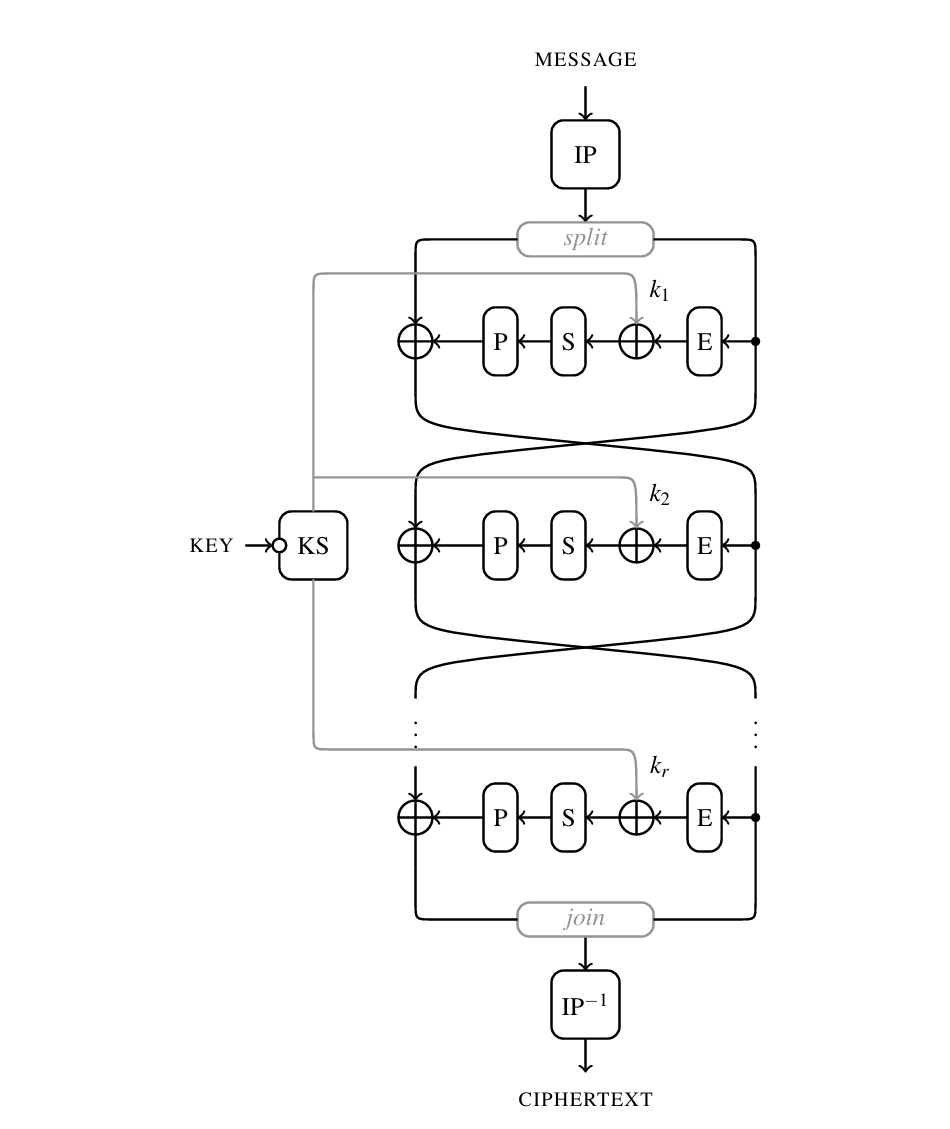
\includegraphics[width=0.5\linewidth]{DES encryption}
\caption{\label{fig:form1} DES encryption [3, p16]}
\end{figure}

The round functions in each round is the same, they first expand the 32-bit half to 48 bits, then operate it with round key by
XOR operation, the 48-bit intermediate value are separated into eight 6-bit words, put each into a different S-boxes, and
the eight outputs of 4-bit are concatenated to form a 32-bit message. At last, the 32-bit message is permuted by
A bit-level permutation (P) and produces the output of the round function.

The S-boxes are the only nonlinear components in DES [3]. Each S-box can be considered as a table of 4 rows and 16 columns, containing values from 0 to 15.
the 6-bit input is split, two outer bits are formed to choose the row of table and the four inner bits are formed to get the
column, the value in that row and column is the 4-bit output of that S-box.

It is worth noticing that DES, as a Feistel cipher, has a decryption process that follows the same procedures as encryption
but use the round keys in reverse order.

\section{DES properties}
In this paper, some important DES properties are implemented and proved with the assistance of HOL4. They are the implementation properties,
weak key and semi-weak key properties.

The DES complementation property [2] is for a plaintext input m and key k, and the bitwise complement of them \verb|~m| and \verb|~k|, the
complement result after encrypting m using DES and k as key is the same as the result after the DES encryption step
using \verb|~w| and \verb|~k| like shown in below.

\begin{equation*}
\begin{split}
   \sim \, \text{DES}_{w}(m) = \text{DES}_{\sim w}(\sim m)
\end{split}
\end{equation*}

By verifying this, we know a limitation of DES, in a chosen message attack
this property can reduce the cost of exhaustive key search by half[2]. It is because to check if one guessing k is right,
one known message and DES encryption can produce two ciphertext c and ~c by applying bitwise complementation to c. This process
equals to two DES encryption for two known messages and keys, the exhaustive search of key of length 56 can reduce from
$2^{55}$ to $2^{54}$.

Weak keys are four special keys follow the property that DES encrypts a message twice with the same weak keys will return
the same message as shown.

\begin{equation*}
\begin{split}
   \text{DES}_{w} \, (\text{DES}_{w}(m)) \;= \;m
\end{split}
\end{equation*}

It is because the weak keys cause round keys equal to  the reverse of
the round keys, cause the DES encryption and decryption to be the same. Weak keys also have the property that each weak key
has corresponding $2^{32}$ messages that encrypt these messages with that weak key will result message unchanged. These messages
have the property that their input halves are the same in the encryption process of the 8th rounds. By combining this with the weak keys' reverse
order round keys property, it ensures the input halves in the (8-n)th and (8+n)th round are the same, result the original message (0th round) the same
as the ciphertext (16th round).

Similarly, semi-weak keys are six key pairs that encrypts a message with one of the key in the pair then encrypts the resulting
ciphertext with the other key in the pair will keep the message unchanged. The formula is shown below.

\begin{equation*}
\begin{split}
   \text{DES}_{w_{1}} \, (\text{DES}_{w_{2}}(m)) \;= \;m
\end{split}
\end{equation*}

The reason
is the same as weak keys, the round keys of the two semi-weak keys in a pair are arranged in the reverse order.

These properties cannot reduce the complexity for exhaustive key search especially for only 4 weak keys compare to the total
of $2^{56}$ keys. However, their existence can be vital when DES is used within some construction[3].

\subsection{DES in HOL4}
DES algorithm has been built in the \verb|desScript| file in HOL4, and my paper build the verifications based on the DES implemented
in this file.

In the file, it first defines some specific types used in
the Data Encryption Standard implementation. It includes the halves of word/plaintext as a pair of word32, halves of
keys in each round as pair of word28 and a function type of S-Box that take word6 as inputs and return
word4. It also includes the data tables to help facilitate the IP, inverse IP permutations, E expansion, P, PC1 and PC2
permutations, round-dependent rotation values and the permutation values for the S-boxes. Then there are
some functions and definitions that perform the expansion, permutations, reversion and the S-Boxes' processing. The ``Key Scheduling'' section
in this file are definitions to build the round keys from the input key. As the last part of preparing, there are
join and split functions to initially split the plaintext and form the result ciphertext. Theorems are also constructed to
verify some basic properties and help ensure the correctness of implementations.

It then actually build the XOR operation, round function and swap operation in each round. Moreover, it combines the above operations, along with the
round keys to form the actual process for each round and ultimately construct the complete DES process over a total of16 rounds.
It also implements a help function that can return the input halves in each round as a pair in the form of \verb|(M a, M b)|. It is beneficial
for any future analysis of DES, including the verification of the proper DES implementation in \verb|desScript| and my additional DES
properties proving. At last, it proved that as a Feistel network, the implemented encryption of DES using the round
keys, followed by a second encryption using the reversed round keys
will return the original plaintext.
%A version of DES with components are shown in Figure~\ref{fig:form2}

%\begin{figure}
%\centering
%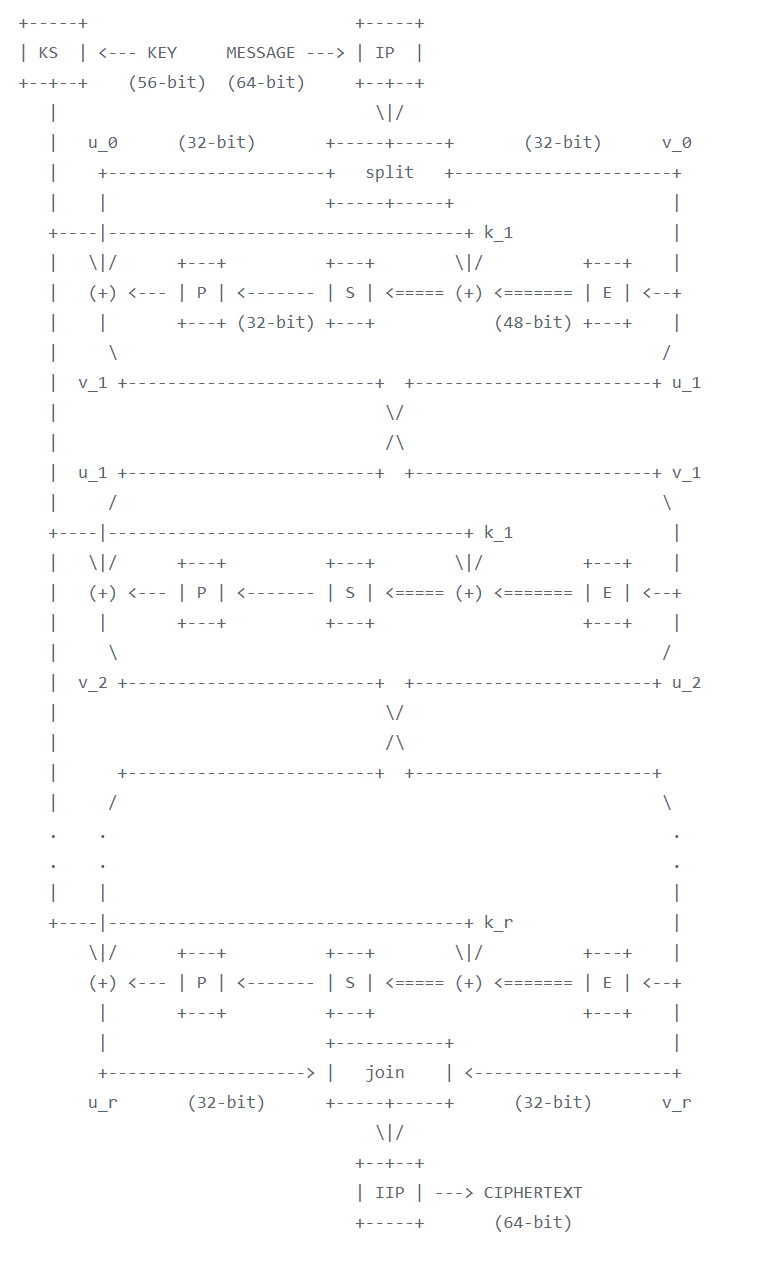
\includegraphics[width=0.5\linewidth]{DES hol4}
%\caption{\label{fig:form2} DES in HOL4 [3, p16]}
%\end{figure}

Consequently, it not only verifies that the decryption of DES is the same process of encryption but with reversed round keys,
but also confirms the correctness of DES implementation in HOL4 by proving that decrypting the encrypted message with the same key
will return the original message.

\section{DES property in HOL4}
In my \verb|des_propScript| file in HOL4, there are some basic settings. It loads all the relevant theories and libraries which contains
necessary definitions and theorems I need to use including the \verb|desScript|. I set the \verb|guessing_word_lengths| to true so that
I do not need to set the length for each word, they will be assigned to a length based on the conditions. Additionally, I also define a simpleset
\verb|fcp_ss|, it is a simplification set that combines \verb|std_ss|, the basic simplification set, with \verb|FCP_ss|, the simpset fragment
specifically simplifies finite Cartesian product expressions.

\subsection{Complementation property}
First of all, I proved the complementation property, it is implemented as the theorem \verb|comple_property|.

\begin{alltt}
\HOLTokenTurnstile{} \HOLSymConst{\HOLTokenForall{}}(\HOLBoundVar{k} :\HOLTyOp{word64}) (\HOLBoundVar{m} :\HOLTyOp{word64}) (\HOLBoundVar{n} :\HOLTyOp{num}).
     (\HOLNumLit{0} :\HOLTyOp{num}) \HOLSymConst{\HOLTokenLt{}} \HOLBoundVar{n} \HOLSymConst{\HOLTokenConj{}} \HOLBoundVar{n} \HOLSymConst{\HOLTokenLt{}} (\HOLNumLit{17} :\HOLTyOp{num}) \HOLSymConst{\HOLTokenConj{}}
     \HOLConst{DES} \HOLBoundVar{n} \HOLBoundVar{k} \HOLSymConst{=}
     ((\HOLFreeVar{encrypt} :\HOLTyOp{word64} \HOLTokenMap{} \HOLTyOp{word64})\HOLSymConst{,}(\HOLFreeVar{decrypt} :\HOLTyOp{word64} \HOLTokenMap{} \HOLTyOp{word64})) \HOLSymConst{\HOLTokenConj{}}
     \HOLConst{DES} \HOLBoundVar{n} (\HOLSymConst{\HOLTokenNeg{}}\HOLBoundVar{k}) \HOLSymConst{=}
     ((\ensuremath{\HOLFreeVar{encrypt}\sp{\prime{}}} :\HOLTyOp{word64} \HOLTokenMap{} \HOLTyOp{word64})\HOLSymConst{,}(\ensuremath{\HOLFreeVar{decrypt}\sp{\prime{}}} :\HOLTyOp{word64} \HOLTokenMap{} \HOLTyOp{word64})) \HOLSymConst{\HOLTokenImp{}}
     \HOLSymConst{\HOLTokenNeg{}}\HOLFreeVar{encrypt} \HOLBoundVar{m} \HOLSymConst{=} \ensuremath{\HOLFreeVar{encrypt}\sp{\prime{}}} (\HOLSymConst{\HOLTokenNeg{}}\HOLBoundVar{m})
\end{alltt}

It means for any key k, message m and number of rounds n, the complementation of encryption using m and k is the
same as the encryption using the complementation of m and k.

I initially convert the \verb|encrypt| function to more detailed components functions including inverse of initial permutation,
join, swap, round, split and initial permutation functions. This allows the use of rewriting rules on separated
functions. This includes some theorems proving the complementation property of each individual function mentioned above.
The below theorem is an example for join function.

\begin{alltt}
\HOLTokenTurnstile{} \HOLSymConst{\HOLTokenForall{}}(\HOLBoundVar{m} :\HOLTyOp{word32}) (\HOLBoundVar{n} :\HOLTyOp{word32}). \HOLConst{Join} (\HOLSymConst{\HOLTokenNeg{}}\HOLBoundVar{m}\HOLSymConst{,}\HOLSymConst{\HOLTokenNeg{}}\HOLBoundVar{n}) \HOLSymConst{=} \HOLSymConst{\HOLTokenNeg{}}\HOLConst{Join} (\HOLBoundVar{m}\HOLSymConst{,}\HOLBoundVar{n})
\end{alltt}

I then convert the \verb|Round| function to the $(M \,a,\; M \,b)$ by the \verb|half_message| help function.

\begin{alltt}
\HOLTokenTurnstile{} \HOLSymConst{\HOLTokenForall{}}(\HOLBoundVar{f} :\ensuremath{\alpha} \HOLTyOp{word} \HOLTokenMap{} \ensuremath{\beta} \HOLTokenMap{} \ensuremath{\alpha} \HOLTyOp{word}) (\HOLBoundVar{u} :\ensuremath{\alpha} \HOLTyOp{word}) (\HOLBoundVar{v} :\ensuremath{\alpha} \HOLTyOp{word})
       (\HOLBoundVar{ks} :\ensuremath{\beta} \HOLTyOp{list}).
     \HOLConst{half_message} \HOLBoundVar{f} (\HOLBoundVar{u}\HOLSymConst{,}\HOLBoundVar{v}) \HOLBoundVar{ks} (\HOLNumLit{0} :\HOLTyOp{num}) \HOLSymConst{=} \HOLBoundVar{u} \HOLSymConst{\HOLTokenConj{}}
     \HOLConst{half_message} \HOLBoundVar{f} (\HOLBoundVar{u}\HOLSymConst{,}\HOLBoundVar{v}) \HOLBoundVar{ks} (\HOLNumLit{1} :\HOLTyOp{num}) \HOLSymConst{=} \HOLBoundVar{v} \HOLSymConst{\HOLTokenConj{}}
     \HOLSymConst{\HOLTokenForall{}}(\HOLBoundVar{n} :\HOLTyOp{num}).
       (\HOLNumLit{2} :\HOLTyOp{num}) \HOLSymConst{\HOLTokenLeq{}} \HOLBoundVar{n} \HOLSymConst{\HOLTokenImp{}}
       \HOLConst{half_message} \HOLBoundVar{f} (\HOLBoundVar{u}\HOLSymConst{,}\HOLBoundVar{v}) \HOLBoundVar{ks} \HOLBoundVar{n} \HOLSymConst{=}
       \HOLConst{half_message} \HOLBoundVar{f} (\HOLBoundVar{u}\HOLSymConst{,}\HOLBoundVar{v}) \HOLBoundVar{ks} (\HOLBoundVar{n} \HOLSymConst{\ensuremath{-}} (\HOLNumLit{2} :\HOLTyOp{num})) \HOLSymConst{\HOLTokenEor{}}
       \HOLBoundVar{f} (\HOLConst{half_message} \HOLBoundVar{f} (\HOLBoundVar{u}\HOLSymConst{,}\HOLBoundVar{v}) \HOLBoundVar{ks} (\HOLBoundVar{n} \HOLSymConst{\ensuremath{-}} (\HOLNumLit{1} :\HOLTyOp{num})))
         (\HOLConst{EL} (\HOLBoundVar{n} \HOLSymConst{\ensuremath{-}} (\HOLNumLit{2} :\HOLTyOp{num})) \HOLBoundVar{ks})
\end{alltt}

As a result, I can research on each 32-bit
half of the block and use the relation between halves in the same and different rounds. Moreover, I simplify the proving goals by rewriting it with the theorems about the complementation
property of each individual function, leave only solving the complementation property of a pair of M function.

\begin{multline*}
(M \; (u', v') \; keys' \; n, \; M \; (u', v') \; keys' \; (SUC \, n)) \\
= (\sim M \; (u, v) \; keys \; n, \; \sim M \; (u, v) \; keys \; (SUC \, n))
\end{multline*}

I decide to use the Mathematical induction method using \verb|Induct_on| in HOL4. I replace the variable n to x, define x to be $<=$ n, and then
perform induction on variable x. It is to avoid the failure of proving the induction step. As the prerequisite of using
given case is $n>0$ , but in the step case, only $(SUC n) > 0$ (SUC means successor) is given. From $n+1 > 0$, it is not possible to
derive the requirement of $n > 0$, thus given case cannot be used, verification cannot be pushed further. By converting to x,
the prerequisites can be easily meet, and facilitating the proof process.

To prove the base case, we only need to convert back to the form of \verb|Round| function and use the base case of the \verb|Round| function.
It is because only \verb|Round| function is built using the relationships between its values based on inductively given inputs, and
it has the base case for $x=0$. To complete the
base case verification, I also prove $(u,\;v)= (u',\;v')$ by extract the abbreviation of them back into their original forms, and apply the complementation rule of
IP function. The abbreviation can be viewed below.

\begin{align*}
\text{Abbrev} \; & (u \;=\; (63 \,><\, 32) \; (IP \,m)) \\
\text{Abbrev} \; & (v \;=\; (31 \,><\, 0) \; (IP \,m)) \\
\text{Abbrev} \; & (u' \;=\; (63 \,><\, 32) \; (IP \,(\sim m))) \\
\text{Abbrev} \; & (v' \;=\; (31 \,><\, 0) \; (IP \,(\sim m)))
\end{align*}


It is important to note that $(M \,a,\;M \,b)$ can be converted from the \verb|Round| function. It is defined as a pair of two
halves taking $n$th round as one of the inputs,
which are the two halves in the n-th round during the DES encryption process. According to the workflow of encryption, the right
half of round $n$ equals to the left half of round $(n+1)$ by the swap operation at the end of each round. Depend on this and the workflow,
the right half of round $(n+1)$ can be expressed as the two halves in previous round with some operations.
By using the relationship of halves between different rounds,
each half of $(M \,a,\;M \,b)$ in round $(n+1)$ can be expressed by the halves in round $n$. Consequently, in the induction step,
the step case which contains $(M \,a,\;M \,b)$ in round $(SUC \,n)$ can be expressed into formulas using $(M \,a,\;M \,b)$ in round
$n$ which are contained in the base case. As a result, I can use the assumptions provided in the base case to push forward my
verification.

\begin{multline*}
Assumption: \quad (M \; (u', v') \; keys' \; x, \; M \; (u', v') \; keys' \; (SUC \, x)) \\
= (\sim M \; (u, v) \; keys \; x, \; \sim M \; (u, v) \; keys \; (SUC \, x))
\end{multline*}

\begin{multline*}
Goal: \quad (M \; (u', v') \; keys' \; (SUC \,x), \; M \; (u', v') \; keys' \; (SUC \,(SUC \, x))) \\
= (\sim M \; (u, v) \; keys \; (SUC \,x), \; \sim M \; (u, v) \; keys \; (SUC \,(SUC \, x)))
\end{multline*}

By the above conversions and simplifications using base case, the proving goal is now transformed to verify only the
complementation property about round function. It is to prove that round function with 32-bite message m and round
key generated by key k equals to the round function with inputs of
the complementation of both m and k. In HOL4, \verb|RoundOp| function is built to represent round function of each round
combining the expansion E, XOR operation with round key, S-boxes permutations S and the bit-level permutation P. By expanding
the \verb|RoundOp| function, the goal can now reduce to:

\begin{multline*}
P \; (S \; (E \;(\sim M \; (u, v) \; keys \; (x+1)) \; \oplus \; (EL \;x \;keys')))\\
= P \; (S \; (E \;(M \; (u, v) \; keys \; (x+1)) \;\oplus \;(EL \;x \;keys)))
\end{multline*}

As the property of exclusive OR operation, $(\sim a) \; \oplus \; (\sim  b) \;= \;a \; \oplus \; b$ and the support
complementation property of the expansion function, $E \; (\sim a) \;= \; \sim  E \; (a)$ once I prove the complementation of
round key generated by key k is equal to the round key generated by the complementation of key k, the verification of complementation property
in DES is done.

The implementation of the design about round key in HOL4 is generated by \verb|RoundKey| and \verb|KS| function. \verb|RoundKey| outputs a
round key list that the elements in it
are pairs of 28-bit words, each pair represents the two halves after the splitting of initial key, the rearrangement by PC1
and the rotation in different rounds. \verb|KS| then using the \verb|MAP| function to map each element in the output of \verb|RoundKey| to
perform PC2 permutations. For convenience in the verification, I define three functions \verb|RK|, \verb|RK_L| and \verb|RK_R|.
\verb|RoundKey| can be converted to \verb|RK| and thus split into $(RK\_L \; a \;,RK\_R \; a)$, and now I can work on each half of the pair
separately, instead of only be able to work on the pair as a whole. The current form of goal can be expressed like:

\begin{multline*}
EL \; x \; (MAP \; f \; (list \; of \; input \; \sim k))\\
= \sim EL \; x \; (MAP \; f \; (list \; of \; input \; k))
\end{multline*}

By applying a series of rewriting rules in \verb|listTheory| that can deal with \verb|EL|, \verb|MAP| and some functions in $f$, the complementation
theorems for \verb|RK_L| and \verb|RK_R|, the goal finally transforms to $MAP\; f \;l = MAP\; f'\; l$. At last, the complementation property of PC2
permutation is used
to finish the proof of $f\;=\;f'$. The initial goal of DES complementation property is proved in HOL4 through the above steps.

As mentioned above, I proved many support theorems about the complementation property of each single operation, their proofs are
done in a similar way. The operations are expanded by their definitions to transform the verification into each bit of $\sim m$
at the permuted indices equals to the complementation of each bit of $m$ in the same indices. For example, the indices of IP
permutation are transformed to $64 \; - \; EL \; (63 \;-\;i) \; IP_{data}$ where $i$ is the original index of m before IP
permutation. $IP_{data}$ is the IP table to do the permutations, and it rearranges the bits in different positions of m
to form a new message. Then I need to prove that the transformed indices are still less than the length of input message m to
meet the prerequisite for using the theorem, \verb|FCP_BETA| and then I can complete the proof.

\begin{alltt}
\HOLTokenTurnstile{} \HOLSymConst{\HOLTokenForall{}}\HOLBoundVar{i}. \HOLBoundVar{i} \HOLSymConst{\HOLTokenLt{}} \HOLConst{dimindex} (:\ensuremath{\beta}) \HOLSymConst{\HOLTokenImp{}} (\HOLSymConst{FCP}) \HOLFreeVar{g} \HOLConst{'} \HOLBoundVar{i} \HOLSymConst{=} \HOLFreeVar{g} \HOLBoundVar{i}
\end{alltt}

The proof that the transformed indices are all less than the length of input message m (64) given $i$ is less than 64 uses
the method of exhaustion. It repeatedly proves the transformed index is less than 64 for each value of i for 64 times, covering
all cases from $i=0$ to $i=63$. The proof is completed as all 64 situations meet the condition. Overall, the support theorems are
all proved with a similar way.

There are some special built-in tactics, conversions used here. The \verb|MATCH_MP_TAC| tactic takes a theorem as input,
it can be applied to the goal if the current goal is in the form of the consequent of this theorem. The goal can then be
converted to the antecedent of the theorem. \verb|rpt| is a tactic that takes a tactic as input and repeatedly apply the tactic until
it no longer succeeds. \verb|CONV_TAC| is a special tactic that makes a tactic from a conversion. Then \verb|BOUNDED_FORALL_CONV| is a
conversion that deal with universal quantification for bounded natural numbers, so it converts $\forall n. \;n \; < \; k$ to
the conjunction of $n=0$ to $n=(k-1)$, like the exhaustion methods for i that I mentioned above.

There are also some theorems and definitions that are frequently used in the proof. \verb|word_1comp_def| defines the complementation of a word m,
$\sim m$ equals to the concentration of the complementation of each bit of word m. It helps deal with the complementation in
bit level.

When dealing with the lists and some operations applies to lists like the map function. \verb|MAP_TL| shows that applying a function
to the tail of a list is equal to the tail of a list after the mapping. Then the theorem \verb|MAP_MAP_o| states applying two functions
to a list using \verb|MAP| twice is equivalent to applying the composition of the two function using \verb|MAP| once.

\begin{alltt}
\HOLTokenTurnstile{} \HOLSymConst{\HOLTokenForall{}}\HOLBoundVar{l} \HOLBoundVar{f}. \HOLConst{MAP} \HOLBoundVar{f} (\HOLConst{TL} \HOLBoundVar{l}) \HOLSymConst{=} \HOLConst{TL} (\HOLConst{MAP} \HOLBoundVar{f} \HOLBoundVar{l})\hfill{[MAP_TL]}
\end{alltt}

\begin{alltt}
\HOLTokenTurnstile{} \HOLSymConst{\HOLTokenForall{}}\HOLBoundVar{f} \HOLBoundVar{g} \HOLBoundVar{l}. \HOLConst{MAP} \HOLBoundVar{f} (\HOLConst{MAP} \HOLBoundVar{g} \HOLBoundVar{l}) \HOLSymConst{=} \HOLConst{MAP} (\HOLBoundVar{f} \HOLSymConst{\HOLTokenCompose} \HOLBoundVar{g}) \HOLBoundVar{l}\hfill{[MAP_MAP_o]}
\end{alltt}

\subsection{Weak and semi-weak key property}
I first define the four weak keys into HOL4 in hexadecimal form. Then I want to prove in HOL4 that for all the DES encryptions using
the weak keys, applying the encryption twice to any message will result the message nochange.

\begin{alltt}
\HOLTokenTurnstile{} \HOLSymConst{\HOLTokenForall{}}(\HOLBoundVar{k} :\HOLTyOp{word64}) (\HOLBoundVar{plaintext} :\HOLTyOp{word64}).
     \HOLConst{MEM} \HOLBoundVar{k} \HOLConst{Wkey} \HOLSymConst{\HOLTokenConj{}}
     \HOLConst{FullDES} \HOLBoundVar{k} \HOLSymConst{=}
     ((\HOLFreeVar{encrypt} :\HOLTyOp{word64} \HOLTokenMap{} \HOLTyOp{word64})\HOLSymConst{,}(\HOLFreeVar{decrypt} :\HOLTyOp{word64} \HOLTokenMap{} \HOLTyOp{word64})) \HOLSymConst{\HOLTokenImp{}}
     \HOLFreeVar{encrypt} (\HOLFreeVar{encrypt} \HOLBoundVar{plaintext}) \HOLSymConst{=} \HOLBoundVar{plaintext}\hfill{[weakK_proper]}
\end{alltt}

It can be proven easily using the existing theorem \verb|desCore_CORRECT| in \verb|desTheory|. DES has the property that
the decryption in DES of a key is the same process of encryption in DES but use the reverse list of round keys generated
from the same key. The \verb|desCore_CORRECT| theorem uses this property and the fact that decrypting an encrypted message
returns the original message. It successfully proves that encryption to a message twice with a key,
once using the normal round keys, once using the round keys in reverse order remains message unchanged.

\begin{alltt}
\HOLTokenTurnstile{} \HOLSymConst{\HOLTokenForall{}}(\HOLBoundVar{keys} :\HOLTyOp{word48} \HOLTyOp{list}) (\HOLBoundVar{r} :\HOLTyOp{num}) (\HOLBoundVar{plaintext} :\HOLTyOp{word64}).
     \HOLConst{LENGTH} \HOLBoundVar{keys} \HOLSymConst{=} \HOLBoundVar{r} \HOLSymConst{\HOLTokenImp{}}
     \HOLConst{desCore} \HOLBoundVar{r} (\HOLConst{REVERSE} \HOLBoundVar{keys}) (\HOLConst{desCore} \HOLBoundVar{r} \HOLBoundVar{keys} \HOLBoundVar{plaintext}) \HOLSymConst{=}
     \HOLBoundVar{plaintext}
\end{alltt}

By applying this to the goal, I am left with only the proofing of the prerequisite of \verb|desCore_CORRECT| and the
proof of round keys list generated by weak key remains the same after being reversed, that is:

\begin{equation*}
   \mathrm{REVERSE} \; (KS \; k \; 16) = KS \; k \; 16
\end{equation*}

The rest part is easy to prove, the length of the list of round keys is equal to the number of rounds by the \verb|LENGTH_KS|
theorem. The equivalent proof about the round keys can be done by substituting each weak key's value into the goal,
use the \verb|EVAL_TAC| that applies the values of keys to the goal and evaluate on the value. The goal is proved after
the successful equation calculation on each value.

\begin{alltt}
\HOLTokenTurnstile{} \HOLSymConst{\HOLTokenForall{}}(\HOLBoundVar{k} :\HOLTyOp{word64}) (\HOLBoundVar{n} :\HOLTyOp{num}). \HOLConst{LENGTH} (\HOLConst{KS} \HOLBoundVar{k} \HOLBoundVar{n}) \HOLSymConst{=} \HOLBoundVar{n}\hfill{[LENGTH_KS]}
\end{alltt}

The semi-weak keys' property and its corresponding verification are similar to weak keys'. I define them as pairs in a list,
set the goal to be: encrypting a message with one key in a pair and encrypting the ciphertext with another key
in that pair make the ciphertext back to the original message.

\begin{alltt}
\HOLTokenTurnstile{} \HOLSymConst{\HOLTokenForall{}}(\HOLBoundVar{plaintext} :\HOLTyOp{word64}) (\HOLBoundVar{pair} :\HOLTyOp{word64} \HOLTokenProd{} \HOLTyOp{word64}).
     \HOLConst{MEM} \HOLBoundVar{pair} \HOLConst{Semiwkey} \HOLSymConst{\HOLTokenConj{}} \HOLBoundVar{pair} \HOLSymConst{=} ((\ensuremath{\HOLFreeVar{s}\sb{\mathrm{1}}} :\HOLTyOp{word64})\HOLSymConst{,}(\ensuremath{\HOLFreeVar{s}\sb{\mathrm{2}}} :\HOLTyOp{word64})) \HOLSymConst{\HOLTokenConj{}}
     \HOLConst{FullDES} \ensuremath{\HOLFreeVar{s}\sb{\mathrm{1}}} \HOLSymConst{=}
     ((\HOLFreeVar{encrypt} :\HOLTyOp{word64} \HOLTokenMap{} \HOLTyOp{word64})\HOLSymConst{,}(\HOLFreeVar{decrypt} :\HOLTyOp{word64} \HOLTokenMap{} \HOLTyOp{word64})) \HOLSymConst{\HOLTokenConj{}}
     \HOLConst{FullDES} \ensuremath{\HOLFreeVar{s}\sb{\mathrm{2}}} \HOLSymConst{=}
     ((\ensuremath{\HOLFreeVar{encrypt}\sp{\prime{}}} :\HOLTyOp{word64} \HOLTokenMap{} \HOLTyOp{word64})\HOLSymConst{,}(\ensuremath{\HOLFreeVar{decrypt}\sp{\prime{}}} :\HOLTyOp{word64} \HOLTokenMap{} \HOLTyOp{word64})) \HOLSymConst{\HOLTokenImp{}}
     \HOLFreeVar{encrypt} (\ensuremath{\HOLFreeVar{encrypt}\sp{\prime{}}} \HOLBoundVar{plaintext}) \HOLSymConst{=} \HOLBoundVar{plaintext}\hfill{[semiK_proper1]}
\end{alltt}

\begin{alltt}
\HOLTokenTurnstile{} \HOLSymConst{\HOLTokenForall{}}(\HOLBoundVar{plaintext} :\HOLTyOp{word64}) (\HOLBoundVar{pair} :\HOLTyOp{word64} \HOLTokenProd{} \HOLTyOp{word64}).
     \HOLConst{MEM} \HOLBoundVar{pair} \HOLConst{Semiwkey} \HOLSymConst{\HOLTokenConj{}} \HOLBoundVar{pair} \HOLSymConst{=} ((\ensuremath{\HOLFreeVar{s}\sb{\mathrm{1}}} :\HOLTyOp{word64})\HOLSymConst{,}(\ensuremath{\HOLFreeVar{s}\sb{\mathrm{2}}} :\HOLTyOp{word64})) \HOLSymConst{\HOLTokenConj{}}
     \HOLConst{FullDES} \ensuremath{\HOLFreeVar{s}\sb{\mathrm{1}}} \HOLSymConst{=}
     ((\HOLFreeVar{encrypt} :\HOLTyOp{word64} \HOLTokenMap{} \HOLTyOp{word64})\HOLSymConst{,}(\HOLFreeVar{decrypt} :\HOLTyOp{word64} \HOLTokenMap{} \HOLTyOp{word64})) \HOLSymConst{\HOLTokenConj{}}
     \HOLConst{FullDES} \ensuremath{\HOLFreeVar{s}\sb{\mathrm{2}}} \HOLSymConst{=}
     ((\ensuremath{\HOLFreeVar{encrypt}\sp{\prime{}}} :\HOLTyOp{word64} \HOLTokenMap{} \HOLTyOp{word64})\HOLSymConst{,}(\ensuremath{\HOLFreeVar{decrypt}\sp{\prime{}}} :\HOLTyOp{word64} \HOLTokenMap{} \HOLTyOp{word64})) \HOLSymConst{\HOLTokenImp{}}
     \ensuremath{\HOLFreeVar{encrypt}\sp{\prime{}}} (\HOLFreeVar{encrypt} \HOLBoundVar{plaintext}) \HOLSymConst{=} \HOLBoundVar{plaintext}\hfill{[semiK_proper2]}
\end{alltt}

The way to achieve this goal only change the part about the equivalent proof of round keys and reversed round keys.
It is now to verify that the round keys generated by one of the semi-weak keys are equal to the revered round
keys generated by the other key. The method of verification is still use \verb|EVAL_TAC| to evaluate on the values of semi-weak
keys. The proof is then done.

\begin{equation*}
\begin{split}
 REVERSE \; (KS \; k1 \; 16)= KS \; k2 \; 16
\end{split}
\end{equation*}

\subsection{Fixed points for DES weak keys}
I can now prove each weak key has $2^{32}$ messages that encrypting these messages with the corresponding weak key remain
the messages unchanged. As mentioned in earlier section, these messages have this property based on their property that
the input halves are the same in round 8 during the DES encryption using the corresponding weak key. Based on this, I define
four sets for four weak keys that each list obtains messages with the above property. I can then prove separately that
all messages in the set meet the property that encryption does not change the message, and each set has cardinality
of $2^{32}$.

\begin{alltt}
\HOLTokenTurnstile{} \HOLSymConst{\HOLTokenForall{}}(\HOLBoundVar{x} :\HOLTyOp{word64}).
     \HOLBoundVar{x} \HOLSymConst{\HOLTokenIn{}} \HOLConst{Wtext1} \HOLSymConst{\HOLTokenConj{}}
     \HOLConst{FullDES} \HOLConst{Wkey1} \HOLSymConst{=}
     ((\HOLFreeVar{encrypt} :\HOLTyOp{word64} \HOLTokenMap{} \HOLTyOp{word64})\HOLSymConst{,}(\HOLFreeVar{decrypt} :\HOLTyOp{word64} \HOLTokenMap{} \HOLTyOp{word64})) \HOLSymConst{\HOLTokenImp{}}
     \HOLFreeVar{encrypt} \HOLBoundVar{x} \HOLSymConst{=} \HOLBoundVar{x}\hfill{[weakK1_proper2]}
\end{alltt}

\begin{alltt}
\HOLTokenTurnstile{} \HOLSymConst{\HOLTokenForall{}}(\HOLBoundVar{x} :\HOLTyOp{word64}).
     \HOLBoundVar{x} \HOLSymConst{\HOLTokenIn{}} \HOLConst{Wtext2} \HOLSymConst{\HOLTokenConj{}}
     \HOLConst{FullDES} \HOLConst{Wkey2} \HOLSymConst{=}
     ((\HOLFreeVar{encrypt} :\HOLTyOp{word64} \HOLTokenMap{} \HOLTyOp{word64})\HOLSymConst{,}(\HOLFreeVar{decrypt} :\HOLTyOp{word64} \HOLTokenMap{} \HOLTyOp{word64})) \HOLSymConst{\HOLTokenImp{}}
     \HOLFreeVar{encrypt} \HOLBoundVar{x} \HOLSymConst{=} \HOLBoundVar{x}\hfill{[weakK2_proper2]}
\end{alltt}

\begin{alltt}
\HOLTokenTurnstile{} \HOLSymConst{\HOLTokenForall{}}(\HOLBoundVar{x} :\HOLTyOp{word64}).
     \HOLBoundVar{x} \HOLSymConst{\HOLTokenIn{}} \HOLConst{Wtext3} \HOLSymConst{\HOLTokenConj{}}
     \HOLConst{FullDES} \HOLConst{Wkey3} \HOLSymConst{=}
     ((\HOLFreeVar{encrypt} :\HOLTyOp{word64} \HOLTokenMap{} \HOLTyOp{word64})\HOLSymConst{,}(\HOLFreeVar{decrypt} :\HOLTyOp{word64} \HOLTokenMap{} \HOLTyOp{word64})) \HOLSymConst{\HOLTokenImp{}}
     \HOLFreeVar{encrypt} \HOLBoundVar{x} \HOLSymConst{=} \HOLBoundVar{x}\hfill{[weakK3_proper2]}
\end{alltt}

\begin{alltt}
\HOLTokenTurnstile{} \HOLSymConst{\HOLTokenForall{}}(\HOLBoundVar{x} :\HOLTyOp{word64}).
     \HOLBoundVar{x} \HOLSymConst{\HOLTokenIn{}} \HOLConst{Wtext4} \HOLSymConst{\HOLTokenConj{}}
     \HOLConst{FullDES} \HOLConst{Wkey4} \HOLSymConst{=}
     ((\HOLFreeVar{encrypt} :\HOLTyOp{word64} \HOLTokenMap{} \HOLTyOp{word64})\HOLSymConst{,}(\HOLFreeVar{decrypt} :\HOLTyOp{word64} \HOLTokenMap{} \HOLTyOp{word64})) \HOLSymConst{\HOLTokenImp{}}
     \HOLFreeVar{encrypt} \HOLBoundVar{x} \HOLSymConst{=} \HOLBoundVar{x}\hfill{[weakK4_proper2]}
\end{alltt}

First, to prove DES encryption with messages in the set remains message unchanged, I expand the goal to more detailed operations
during the DES encryption process. I find that only
if I proved that the reverse of the halves in round 16 during the encryption process are equal to the halves in round 0,
the rest of the proof is
quite simple. I can use the halves in round 0 which do not process any round function, but only the inital IP permutation
and splitting to simplify the goal to:

\begin{equation*}
\begin{split}
 IIP \; (Join \; (Split \; (IP \; x))) \; = \; x
\end{split}
\end{equation*}

These operations can be easily cancelled out by each other using theorem \verb|IIP_IP_Inverse| nad \verb|Join_Split_Inverse|.

\begin{alltt}
\HOLTokenTurnstile{} \HOLSymConst{\HOLTokenForall{}}(\HOLBoundVar{w} :\HOLTyOp{word64}). \HOLConst{IIP} (\HOLConst{IP} \HOLBoundVar{w}) \HOLSymConst{=} \HOLBoundVar{w}\hfill{[IIP_IP_Inverse]}
\end{alltt}

\begin{alltt}
\HOLTokenTurnstile{} \HOLSymConst{\HOLTokenForall{}}(\HOLBoundVar{w} :\HOLTyOp{word64}). \HOLConst{Join} (\HOLConst{Split} \HOLBoundVar{w}) \HOLSymConst{=} \HOLBoundVar{w}\hfill{[Join_Split_Inverse]}
\end{alltt}

I am now left to prove the support theorem \verb|weakK_sup| given the property of each set. It is hard to compare two pairs of
halves that differ by sixteen rounds of operations directly. To achieve the goal in HOL4, I build the support theorem
\verb|weakK_sup| by setting the goal to show that for be each pair of halves in (8-n) round is equal to the reversed pair
in round (8+n). I can then use proof by induction on $n$ to complete the proof.

\begin{alltt}
\HOLTokenTurnstile{} \HOLSymConst{\HOLTokenForall{}}(\HOLBoundVar{n} :\HOLTyOp{num}) (\HOLBoundVar{k} :\HOLTyOp{word64}).
     \HOLConst{MEM} \HOLBoundVar{k} \HOLConst{Wkey} \HOLSymConst{\HOLTokenConj{}} (\HOLNumLit{0} :\HOLTyOp{num}) \HOLSymConst{\HOLTokenLeq{}} \HOLBoundVar{n} \HOLSymConst{\HOLTokenConj{}} \HOLBoundVar{n} \HOLSymConst{\HOLTokenLeq{}} (\HOLNumLit{8} :\HOLTyOp{num}) \HOLSymConst{\HOLTokenConj{}}
     \HOLConst{Split} (\HOLConst{IP} (\HOLConst{desCore} (\HOLNumLit{8} :\HOLTyOp{num}) (\HOLConst{KS} \HOLBoundVar{k} (\HOLNumLit{8} :\HOLTyOp{num})) (\HOLFreeVar{x} :\HOLTyOp{word64}))) \HOLSymConst{=}
     ((\HOLFreeVar{w} :\HOLTyOp{word32})\HOLSymConst{,}\HOLFreeVar{w}) \HOLSymConst{\HOLTokenImp{}}
     \HOLConst{Round} ((\HOLNumLit{8} :\HOLTyOp{num}) \HOLSymConst{\ensuremath{-}} \HOLBoundVar{n}) (\HOLConst{KS} \HOLBoundVar{k} (\HOLNumLit{16} :\HOLTyOp{num})) (\HOLConst{Split} (\HOLConst{IP} \HOLFreeVar{x})) \HOLSymConst{=}
     \HOLConst{Swap}
       (\HOLConst{Round} ((\HOLNumLit{8} :\HOLTyOp{num}) \HOLSymConst{\ensuremath{+}} \HOLBoundVar{n}) (\HOLConst{KS} \HOLBoundVar{k} (\HOLNumLit{16} :\HOLTyOp{num})) (\HOLConst{Split} (\HOLConst{IP} \HOLFreeVar{x})))\hfill{[weakK_sup]}
\end{alltt}

As I define the message sets using round keys list contains only up to the $8th$ round to facilitate future verification,
I first prove that doing the encryption with only 8 round keys is the same as encrypt with all 16 round keys
when just encrypting for 8 rounds by another support theorem. By using it, I convert the prerequisite to mathch the
round keys list with the goal.

Then I start the induction on n and the base case is to prove the two equal input halves $(w\;,\;w)$ at round n is the same after
swapping. It is straightforward, and I only need to expand the \verb|Round| function to pair form and apply the \verb|Swap| definition.

For the induction step, I know the base case shows that the reversed halves in round $a$ $(Ra\;,\; La)$ are equal to
the halves in round $b$ $(Lb\;,\;Rb)$ where $a$ and $b$ represents $(8+n)$ and $(8-n)$.
To proving the step case, I can directly get the right half of round $(b-1)$ $R(b-1)$ is equal to the left half of round $b$
$Lb$ and
the left half of round $(a+1)$ $L(a+1)$ is equal to the right half of round $a$ $Ra$ because only swap operation happens on
these halves between rounds. As $Ra\;= \; Lb$ by the base case, I can get $R(b-1)$ and $L(a+1)$ are the same.
Then because the encryption and decryption process of DES are the same, I can get $L(b-1)$ back from halves in round $b$ through
the round function $f(b-1)$ by using the swap operation, round function and XOR operation

\begin{equation*}
\begin{split}
   L(b-1) \; = \; (Rb \; \oplus \; f(b-1)\,(\;Lb\;)
\end{split}
\end{equation*}
$R(a+1)$ can also be represented by $Ra$ and $La$ in normal encryption manner through the round function $f(a+1)$

\begin{equation*}
\begin{split}
   R(a+1) \; = \; La \; \oplus \; f(a+1)\,(\;Ra\;)
\end{split}
\end{equation*}
According to the proof
done above that round keys list generated by a weak key remains the same after being reversed, I can conclude that the list
is  symmetric, and thus the $(b-1)$th and $(a+1)$th round keys are the same in the round keys list of length 16.
The round function $f(b-1)$ and $f(a+1)$ are then the same as round key is the only change variable for round functions in different
rounds. By combining this with $Rb\;= \; La$ and $Lb\;= \; Ra$, $L(b-1)$ and $R(a+1)$ are the same, and we can prove the step
case is also right given the base case.

Using the above way in HOL4, I convert the goal to halves using $(M\;a\;,\;M\;b)$ function and then
express the step case' halves using the base cases' halves. The only goal left is the proof of the elements in
symmetric positions are the same. I need to put each weak key's value into the goal, calculate the generated
round keys list for each key, ensure the step case's index do not exceed the length of list. At last, I need to
do the method of exhaustion, examine each possible value of n from 0 to 15 to check if they meet the goal because of
the lack of theorems in HOL4 on this aspect. The support theorem is proved.

\begin{equation*}
\begin{split}
 EL \; (7-n) \; (KS \; k \; 16) = EL \; (n+8) \; (KS \; k \; 16)
\end{split}
\end{equation*}
Switch to the last support theorem \verb|wkey1_equal| mentioned above. It is also proved by induction, the base case can
be directly proved by the base case of \verb|Round|. The indcution step is proved in the same way as above by transforming
the \verb|Round| function to $(M\;a\;,\;M\;b)$ form first and then express the step case' halves using the base cases' halves.
The last part of verification is also examine each possible value of n to the goal, use the method of exhaustion to
test all situations meet the goal and the theorem is proved.

\begin{alltt}
\HOLTokenTurnstile{} \HOLSymConst{\HOLTokenForall{}}(\HOLBoundVar{x} :\HOLTyOp{word64}) (\HOLBoundVar{n} :\HOLTyOp{num}) (\HOLBoundVar{k} :\HOLTyOp{word64}).
     \HOLConst{MEM} \HOLBoundVar{k} \HOLConst{Wkey} \HOLSymConst{\HOLTokenConj{}} \HOLBoundVar{n} \HOLSymConst{\HOLTokenLeq{}} (\HOLNumLit{8} :\HOLTyOp{num}) \HOLSymConst{\HOLTokenImp{}}
     \HOLConst{Round} \HOLBoundVar{n} (\HOLConst{KS} \HOLBoundVar{k} (\HOLNumLit{8} :\HOLTyOp{num})) (\HOLConst{Split} \HOLBoundVar{x}) \HOLSymConst{=}
     \HOLConst{Round} \HOLBoundVar{n} (\HOLConst{KS} \HOLBoundVar{k} (\HOLNumLit{16} :\HOLTyOp{num})) (\HOLConst{Split} \HOLBoundVar{x})\hfill{[wkey1_equal]}
\end{alltt}

It is time to prove that the cardinality of the sets of these messages is $2^{32}$. I show these sets form bijection with
the universal set of 32-bit words first. To achieve these, I define two functions for each set, one of the two can map the messages
set to the universal set and the other can map reversely.

\begin{alltt}
\HOLTokenTurnstile{} \HOLConst{BIJ} \HOLConst{w1trans1} \HOLConst{Wtext1} \ensuremath{{\cal{U}}}(:\HOLTyOp{word32})\hfill{[BIJ_wtext1]}
\end{alltt}

\begin{alltt}
\HOLTokenTurnstile{} \HOLConst{BIJ} \HOLConst{w2trans1} \HOLConst{Wtext2} \ensuremath{{\cal{U}}}(:\HOLTyOp{word32})\hfill{[BIJ_wtext2]}
\end{alltt}

\begin{alltt}
\HOLTokenTurnstile{} \HOLConst{BIJ} \HOLConst{w3trans1} \HOLConst{Wtext3} \ensuremath{{\cal{U}}}(:\HOLTyOp{word32})\hfill{[BIJ_wtext3]}
\end{alltt}

\begin{alltt}
\HOLTokenTurnstile{} \HOLConst{BIJ} \HOLConst{w4trans1} \HOLConst{Wtext4} \ensuremath{{\cal{U}}}(:\HOLTyOp{word32})\hfill{[BIJ_wtext4]}
\end{alltt}

To prove the bijection relation between the two sets, \verb|BIJ_IFF_INV| theorem can be used to convert the \verb|BIJ| function into
four sub-goals. It includes proving that all elements in messages set belongs to the other universal set of word32 after mapping,
and vice versa. Moreover, the other two goals are applying the two functions together to the sets will keep the elements unchanged.

\begin{alltt}
\HOLTokenTurnstile{} \HOLSymConst{\HOLTokenForall{}}\HOLBoundVar{f} \HOLBoundVar{s} \HOLBoundVar{t}.
     \HOLConst{BIJ} \HOLBoundVar{f} \HOLBoundVar{s} \HOLBoundVar{t} \HOLSymConst{\HOLTokenEquiv{}}
     (\HOLSymConst{\HOLTokenForall{}}\HOLBoundVar{x}. \HOLBoundVar{x} \HOLSymConst{\HOLTokenIn{}} \HOLBoundVar{s} \HOLSymConst{\HOLTokenImp{}} \HOLBoundVar{f} \HOLBoundVar{x} \HOLSymConst{\HOLTokenIn{}} \HOLBoundVar{t}) \HOLSymConst{\HOLTokenConj{}}
     \HOLSymConst{\HOLTokenExists{}}\HOLBoundVar{g}. (\HOLSymConst{\HOLTokenForall{}}\HOLBoundVar{x}. \HOLBoundVar{x} \HOLSymConst{\HOLTokenIn{}} \HOLBoundVar{t} \HOLSymConst{\HOLTokenImp{}} \HOLBoundVar{g} \HOLBoundVar{x} \HOLSymConst{\HOLTokenIn{}} \HOLBoundVar{s}) \HOLSymConst{\HOLTokenConj{}} (\HOLSymConst{\HOLTokenForall{}}\HOLBoundVar{x}. \HOLBoundVar{x} \HOLSymConst{\HOLTokenIn{}} \HOLBoundVar{s} \HOLSymConst{\HOLTokenImp{}} \HOLBoundVar{g} (\HOLBoundVar{f} \HOLBoundVar{x}) \HOLSymConst{=} \HOLBoundVar{x}) \HOLSymConst{\HOLTokenConj{}}
         \HOLSymConst{\HOLTokenForall{}}\HOLBoundVar{x}. \HOLBoundVar{x} \HOLSymConst{\HOLTokenIn{}} \HOLBoundVar{t} \HOLSymConst{\HOLTokenImp{}} \HOLBoundVar{f} (\HOLBoundVar{g} \HOLBoundVar{x}) \HOLSymConst{=} \HOLBoundVar{x}\hfill{[BIJ_IFF_INV]}
\end{alltt}

Taking the example for proving the first weak key, and the other weak keys are all proved in the same way. Their corresponding
sets and functions just change the weak key used.
The first sub-goal that all elements in messages set belongs to the other universal set of word32 after function \verb|w1trans1| is
proved directly. It takes the 64-bit messages as inputs and outputs only the first reversed halves of message encrypted by 8
rounds. As the outputs are 32 bits, they surely belong to the universal set of word32.

\begin{alltt}
\HOLTokenTurnstile{} \HOLSymConst{\HOLTokenForall{}}(\HOLBoundVar{x} :\HOLTyOp{word64}).
     \HOLConst{w1trans1} \HOLBoundVar{x} \HOLSymConst{=}
     \HOLConst{FST} (\HOLConst{Split} (\HOLConst{IP} (\HOLConst{desCore} (\HOLNumLit{8} :\HOLTyOp{num}) (\HOLConst{KS} \HOLConst{Wkey1} (\HOLNumLit{8} :\HOLTyOp{num})) \HOLBoundVar{x})))\hfill{[w1trans1_def]}
\end{alltt}

The second sub-goal can be converted using definition of function \verb|w1trans2| and set \verb|Wtext1|. All 32-bit messages
(in universal set of word32) are formed as a pair of equal halves, applied with \verb|Join| and \verb|IIP| operation, encrypted
for 8 rounds twice, and applied with \verb|IP| and \verb|Split| operation. And to prove the result halves are still the same.

\begin{alltt}
\HOLTokenTurnstile{} \HOLSymConst{\HOLTokenForall{}}(\HOLBoundVar{x} :\HOLTyOp{word32}).
     \HOLConst{w1trans2} \HOLBoundVar{x} \HOLSymConst{=}
     \HOLConst{desCore} (\HOLNumLit{8} :\HOLTyOp{num}) (\HOLConst{KS} \HOLConst{Wkey1} (\HOLNumLit{8} :\HOLTyOp{num})) (\HOLConst{IIP} (\HOLConst{Join} (\HOLBoundVar{x}\HOLSymConst{,}\HOLBoundVar{x})))\hfill{[w1trans2_def]}
\end{alltt}

\begin{alltt}
\HOLTokenTurnstile{} \HOLConst{Wtext1} \HOLSymConst{=}
   \HOLTokenLeftbrace{}\HOLBoundVar{x} \HOLTokenBar{}
    \HOLSymConst{\HOLTokenExists{}}(\HOLBoundVar{w} :\HOLTyOp{word32}).
      \HOLConst{Split} (\HOLConst{IP} (\HOLConst{desCore} (\HOLNumLit{8} :\HOLTyOp{num}) (\HOLConst{KS} \HOLConst{Wkey1} (\HOLNumLit{8} :\HOLTyOp{num})) \HOLBoundVar{x})) \HOLSymConst{=}
      (\HOLBoundVar{w}\HOLSymConst{,}\HOLBoundVar{w})\HOLTokenRightbrace{}\hfill{[Wtext1_def]}
\end{alltt}

I can also use the previous method to help the proof, the two encryptions of 8 rounds with the weak key cancel each other out
as one of the encryption can be treated as decryption. The \verb|Split| and \verb|Join| operations can be cancelled out, and also the
\verb|IP| and \verb|IIP| operations, results the initial pair of haves unchanged, so the two halves must remain the same with no change.
The second sub-goal is then proved.

The third sub-goal is to prove for an element in the messages' set with the described property, when they are converted
tp the 32-bit half through \verb|w1trans1|, formed as a pair of equal halves and map with the \verb|w1trans2|, the result messages
remain the same. Assumption means x is in the messages' set, goal is to prove the messages remain unchange.

\begin{equation*}
\begin{split}
 Assumption: \text{Split} \; (IP \,(\text{desCore} \,8 \,(\text{KS} \,Wkey1 \,8) \,x)) &= (w, w)
\end{split}
\end{equation*}

\begin{equation*}
\begin{split}
 Goal: \text{desCore} \,8 \,(\text{KS} \,Wkey1 \,8) \,(\text{IIP} \,(\text{Join} \,(w, w))) &= x
\end{split}
\end{equation*}

It proves with the same way as sub-goal 2, but begins to cancel out the \verb|Join| and \verb|Split| operation first, then
the \verb|IIP| and \verb|IP| operations and at last the two encryption processes with weak key. It also cancels each other out,
but in a different order.

The elements are initially in the universal set, change to pairs equal halves, and apply the \verb|w1trans2| function followed
by the \verb|w1trans1| function in the last sub-goal. It can also be verified by cancelling each operations in another order.
The bijection relation between two sets is finally proved.

The bijection proofs for the other three keys are exactly the same, so one proof \verb|BIJ_for_weak_keys_explicit| with the lists of sets, functions and
weak keys as inputs can be done using the existing seperate BIJ theorems.

\begin{alltt}
\HOLTokenTurnstile{} \HOLSymConst{\HOLTokenForall{}}(\HOLBoundVar{i} :\HOLTyOp{num}).
     \HOLBoundVar{i} \HOLSymConst{\HOLTokenLt{}} (\HOLNumLit{4} :\HOLTyOp{num}) \HOLSymConst{\HOLTokenImp{}}
     \HOLConst{BIJ} (\HOLConst{EL} \HOLBoundVar{i} \HOLConst{wtrans1}) (\HOLConst{EL} \HOLBoundVar{i} \HOLConst{Wtextlist}) \ensuremath{{\cal{U}}}(:\HOLTyOp{word32})\hfill{[BIJ_for_weak_keys_explicit]}
\end{alltt}

The universal set of word32 has the cardinality of $2^{32}$ by the theorem \\
\verb|card_word32|. As a result, by proving that
these sets have the same cardinality as the universal set of word32, I can then prove the cardinality of each message set
is $2^{32}$. I can meet the prerequisites that the universal set of word32 is finite directly and use the above
bijection relation, then theorem \verb|FINITE_BIJ_CARD| can be used to prove the equivalence of cardinality.

\begin{alltt}
\HOLTokenTurnstile{} \HOLConst{CARD} \ensuremath{{\cal{U}}}(:\HOLTyOp{word32}) \HOLSymConst{=} (((\HOLNumLit{2} :\HOLTyOp{num}) \HOLSymConst{\HOLTokenExp{}} (\HOLNumLit{32} :\HOLTyOp{num})) :\HOLTyOp{num})\hfill{[card_word32]}
\end{alltt}

\begin{alltt}
\HOLTokenTurnstile{} \HOLSymConst{\HOLTokenForall{}}\HOLBoundVar{f} \HOLBoundVar{s} \HOLBoundVar{t}. \HOLConst{FINITE} \HOLBoundVar{s} \HOLSymConst{\HOLTokenConj{}} \HOLConst{BIJ} \HOLBoundVar{f} \HOLBoundVar{s} \HOLBoundVar{t} \HOLSymConst{\HOLTokenImp{}} \HOLConst{CARD} \HOLBoundVar{s} \HOLSymConst{=} \HOLConst{CARD} \HOLBoundVar{t}\hfill{[FINITE_BIJ_CARD]}
\end{alltt}

As a result, each message set is proved with cardinality of $2^{32}$ and the theorem is stored as
\verb|DES_weak_fp_card| in \verb|des_propTheory|.

\begin{alltt}
\HOLTokenTurnstile{} \HOLSymConst{\HOLTokenForall{}}(\HOLBoundVar{x} :\HOLTyOp{word64} \HOLTokenMap{} \HOLTyOp{bool}).
     \HOLConst{MEM} \HOLBoundVar{x} \HOLConst{Wtextlist} \HOLSymConst{\HOLTokenImp{}} \HOLConst{CARD} \HOLBoundVar{x} \HOLSymConst{=} (((\HOLNumLit{2} :\HOLTyOp{num}) \HOLSymConst{\HOLTokenExp{}} (\HOLNumLit{32} :\HOLTyOp{num})) :\HOLTyOp{num})\hfill{[DES_weak_fp_card]}
\end{alltt}

There are also some new tactics used here to help complete the goal. \\
\verb|Q.PAT_X_ASSUM (Assump) MP_TAC|, it takes a
assumption of current goal \verb|Assump| as input, find the first matching assumption, remove the assumption and take it
as a prerequisite for the current goal. It has similar use as \verb|POP_ASSUM MP_TAC| but avoid the repeat usage
of \verb|POP_ASSUM MP_TAC| when there are too many assumptions.

The \verb|Q.EXISTS_TAC| tactic can be applied to existentially quantified goal. It can substitute a specific term I decide $u$
to the existentially quantified variable $?x$ in the goal. The proof is now changed on $u$.

\section{Differential Cryptanalysis in HOL4}
Differential crypatanalysis of DES-like cryptosystem is a type of cryptanalytic attack which can break reduced variant
of DES up to 15 rounds.[4] Differential crypatanalysis is a chosen-plaintext attack, it can only be used when attackers
are able to encrypt any plaintext using DES encryption and get the corresponding ciphertexts. It can break any variant DES
by attempting the DES encryptions for at most $2^{56}$ time with at most $2^{56}$ plaintexts. The Differential cryptanalysis
attack is developed by the differences in plaintext pairs and differences of ciphertext pairs.

As my current research on differential cryptanalysis is just beginning, the following discussion will be limited within
a single round of DES. The plaintext pairs are two 32-bit message inputs that are passed through the round function
in a round. The ciphertext pairs are the outputs of two round functions using the plaintexts pair in that round.
As S-boxes part is the only nonlinear components of the cipher in DES [3], for pairs of plaintext with fixed
exclusive-or differences, the differences will only change to uncertain values through S-boxes. Other than S-boxes,
the expansion operation and the bit-level permutation $P$ change the \verb|XOR| value to another fixed $values$. For the \verb|XOR| value
of two messages after applying \verb|XOR| operation to them separately with the same round keys, the result value remains the same
difference value. These properties are implemented and proved in HOL4.

\begin{alltt}
  \HOLTokenTurnstile{} \HOLSymConst{\HOLTokenForall{}}(\ensuremath{\HOLBoundVar{x}\sb{\mathrm{1}}} :\HOLTyOp{word32}) (\ensuremath{\HOLBoundVar{x}\sb{\mathrm{2}}} :\HOLTyOp{word32}). \HOLConst{P} \ensuremath{\HOLBoundVar{x}\sb{\mathrm{1}}} \HOLSymConst{\HOLTokenEor{}} \HOLConst{P} \ensuremath{\HOLBoundVar{x}\sb{\mathrm{2}}} \HOLSymConst{=} \HOLConst{P} (\ensuremath{\HOLBoundVar{x}\sb{\mathrm{1}}} \HOLSymConst{\HOLTokenEor{}} \ensuremath{\HOLBoundVar{x}\sb{\mathrm{2}}})\hfill{[xor_P]}
\end{alltt}

\begin{alltt}
  \HOLTokenTurnstile{} \HOLSymConst{\HOLTokenForall{}}(\ensuremath{\HOLBoundVar{x}\sb{\mathrm{1}}} :\HOLTyOp{word32}) (\ensuremath{\HOLBoundVar{x}\sb{\mathrm{2}}} :\HOLTyOp{word32}). \HOLConst{E} \ensuremath{\HOLBoundVar{x}\sb{\mathrm{1}}} \HOLSymConst{\HOLTokenEor{}} \HOLConst{E} \ensuremath{\HOLBoundVar{x}\sb{\mathrm{2}}} \HOLSymConst{=} \HOLConst{E} (\ensuremath{\HOLBoundVar{x}\sb{\mathrm{1}}} \HOLSymConst{\HOLTokenEor{}} \ensuremath{\HOLBoundVar{x}\sb{\mathrm{2}}})\hfill{[xor_E]}
\end{alltt}

\begin{alltt}
  \HOLTokenTurnstile{} \HOLSymConst{\HOLTokenForall{}}(\ensuremath{\HOLBoundVar{x}\sb{\mathrm{1}}} :\ensuremath{\alpha} \HOLTyOp{word}) (\ensuremath{\HOLBoundVar{x}\sb{\mathrm{2}}} :\ensuremath{\alpha} \HOLTyOp{word}) (\HOLBoundVar{k} :\ensuremath{\alpha} \HOLTyOp{word}).
     (\ensuremath{\HOLBoundVar{x}\sb{\mathrm{1}}} \HOLSymConst{\HOLTokenEor{}} \HOLBoundVar{k}) \HOLSymConst{\HOLTokenEor{}} \ensuremath{\HOLBoundVar{x}\sb{\mathrm{2}}} \HOLSymConst{\HOLTokenEor{}} \HOLBoundVar{k} \HOLSymConst{=} \ensuremath{\HOLBoundVar{x}\sb{\mathrm{1}}} \HOLSymConst{\HOLTokenEor{}} \ensuremath{\HOLBoundVar{x}\sb{\mathrm{2}}}\hfill{[xor_twice]}
\end{alltt}

\begin{alltt}
  \HOLTokenTurnstile{} \HOLSymConst{\HOLTokenForall{}}(\HOLBoundVar{Sbox} :\HOLTyOp{sbox}). \HOLSymConst{\HOLTokenExists{}}(\ensuremath{\HOLBoundVar{x}\sb{\mathrm{1}}} :\HOLTyOp{word6}) (\ensuremath{\HOLBoundVar{x}\sb{\mathrm{2}}} :\HOLTyOp{word6}).
     \HOLConst{MEM} \HOLBoundVar{Sbox} \HOLConst{S_list} \HOLSymConst{\HOLTokenImp{}} \HOLBoundVar{Sbox} \ensuremath{\HOLBoundVar{x}\sb{\mathrm{1}}} \HOLSymConst{\HOLTokenEor{}} \HOLBoundVar{Sbox} \ensuremath{\HOLBoundVar{x}\sb{\mathrm{2}}} \HOLSymConst{\HOLTokenNotEqual{}} \HOLBoundVar{Sbox} (\ensuremath{\HOLBoundVar{x}\sb{\mathrm{1}}} \HOLSymConst{\HOLTokenEor{}} \ensuremath{\HOLBoundVar{x}\sb{\mathrm{2}}})\hfill{[xor_Sbox]}
\end{alltt}

The way to prove them is similar to the proof of the complementation property of these operations. I want to prove for each
bit of x1 and x2 after the permutation, each exclusive-or value of the bit pairs is equivalent to the bit value after the
permutation for exclusive-or x1 and x2. The first thing needs to do is to check if the permuted bit indices
are still less than the length of words. Then I expand the definitions of P and E operations, bring in the P and E permutation
tables, and use the method of exhaustion to test on each bit from 0 to the length of output. Since the permuted indices are all
less than the length in all cases, the verification is succeeded. At last, by using the definition of \verb|XOR| in HOL4 that
state applying \verb|XOR| operation to two words means applying \verb|XOR| operation to each bit of two words and \verb|FCP_BETA| that simplify
the $FCP$ out, the proof is done.

\begin{alltt}
  \HOLTokenTurnstile{} \HOLSymConst{\HOLTokenForall{}}(\HOLBoundVar{v} :\ensuremath{\alpha} \HOLTyOp{word}) (\HOLBoundVar{w} :\ensuremath{\alpha} \HOLTyOp{word}).
     \HOLBoundVar{v} \HOLSymConst{\HOLTokenEor{}} \HOLBoundVar{w} \HOLSymConst{=} (\HOLConst{FCP}(\HOLBoundVar{i} :\HOLTyOp{num}). \HOLBoundVar{v} \HOLConst{'} \HOLBoundVar{i} \HOLSymConst{\HOLTokenNotEquiv{}} \HOLBoundVar{w} \HOLConst{'} \HOLBoundVar{i})\hfill{[word_xor_def]}
\end{alltt}

Proving \verb|xor_twice| theorem uses the commutative property of \verb|XOR| and the property that applying \verb|XOR| operations
to a value with itself will cancel out the value.

\begin{alltt}
  \HOLTokenTurnstile{} \HOLSymConst{\HOLTokenForall{}}\HOLBoundVar{a} \HOLBoundVar{b} \HOLBoundVar{c}. (\HOLBoundVar{a} \HOLSymConst{\HOLTokenEor{}} \HOLBoundVar{b}) \HOLSymConst{\HOLTokenEor{}} \HOLBoundVar{c} \HOLSymConst{=} \HOLBoundVar{a} \HOLSymConst{\HOLTokenEor{}} \HOLBoundVar{b} \HOLSymConst{\HOLTokenEor{}} \HOLBoundVar{c}\hfill{[WORD_XOR_ASSOC]}
\end{alltt}

\begin{alltt}
  \HOLTokenTurnstile{} \HOLSymConst{\HOLTokenForall{}}\HOLBoundVar{a}. \HOLConst{UINT_MAXw} \HOLSymConst{\HOLTokenEor{}} \HOLBoundVar{a} \HOLSymConst{=} \HOLSymConst{\HOLTokenNeg{}}\HOLBoundVar{a} \HOLSymConst{\HOLTokenConj{}} \HOLBoundVar{a} \HOLSymConst{\HOLTokenEor{}} \HOLConst{UINT_MAXw} \HOLSymConst{=} \HOLSymConst{\HOLTokenNeg{}}\HOLBoundVar{a} \HOLSymConst{\HOLTokenConj{}} 0w \HOLSymConst{\HOLTokenEor{}} \HOLBoundVar{a} \HOLSymConst{=} \HOLBoundVar{a} \HOLSymConst{\HOLTokenConj{}}
       \HOLBoundVar{a} \HOLSymConst{\HOLTokenEor{}} 0w \HOLSymConst{=} \HOLBoundVar{a} \HOLSymConst{\HOLTokenConj{}} \HOLBoundVar{a} \HOLSymConst{\HOLTokenEor{}} \HOLBoundVar{a} \HOLSymConst{=} 0w\hfill{[WORD_XOR_CLAUSES]}
\end{alltt}

To prove the S-boxes are not linear is much simpler. I choose two words $0b0w$ and $0b0w$ to prove that there exist values
showing S-boxes do not have additivity for \verb|XOR| operation.

As the non-linearity of S-boxes, for pairs of plaintexts with the same \verb|XOR| difference, the output \verb|XOR| differences are
different after the S-boxes if the pairs of plaintexts are different. I can then find a set of pairs of \verb|XOR|$ed$ texts
$(z\;, \;z')$ that
the difference value between them and the difference value after the S-boxes are fixed $\alpha$ and $\beta$. Figure~\ref{fig:form6}
shows the structure of it.

\begin{figure}
\centering
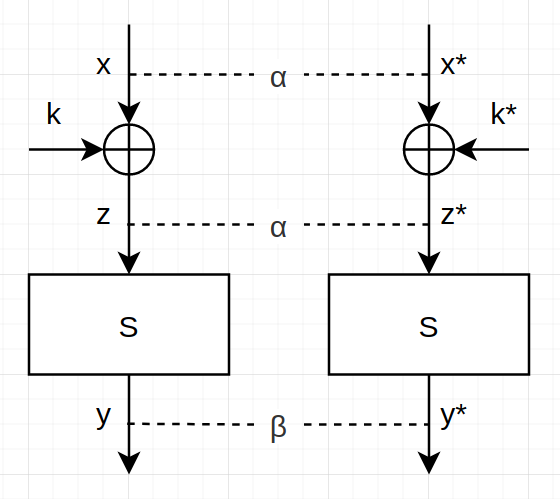
\includegraphics[width=0.5\linewidth]{Sboxdc}
\caption{\label{fig:form6} Differential cryptanalysis for S-boxes}
\end{figure}

The difference value $\alpha$ is the value after expansion. As the additivity for \verb|XOR| operation in expansion function,
a fixed difference value before expansion can produce this value. Similar to the ouput difference values $\beta$ I
choose, they are values before the permutation $P$. As the additivity for \verb|XOR| operation in it, only the inputs used to
generate the sets are changed and the effect can be eliminated by changing the inputs. The inputs are chosen like that
for facilitating the process and match with the table provided in Figure~\ref{fig:form5}.

\begin{figure}
\centering
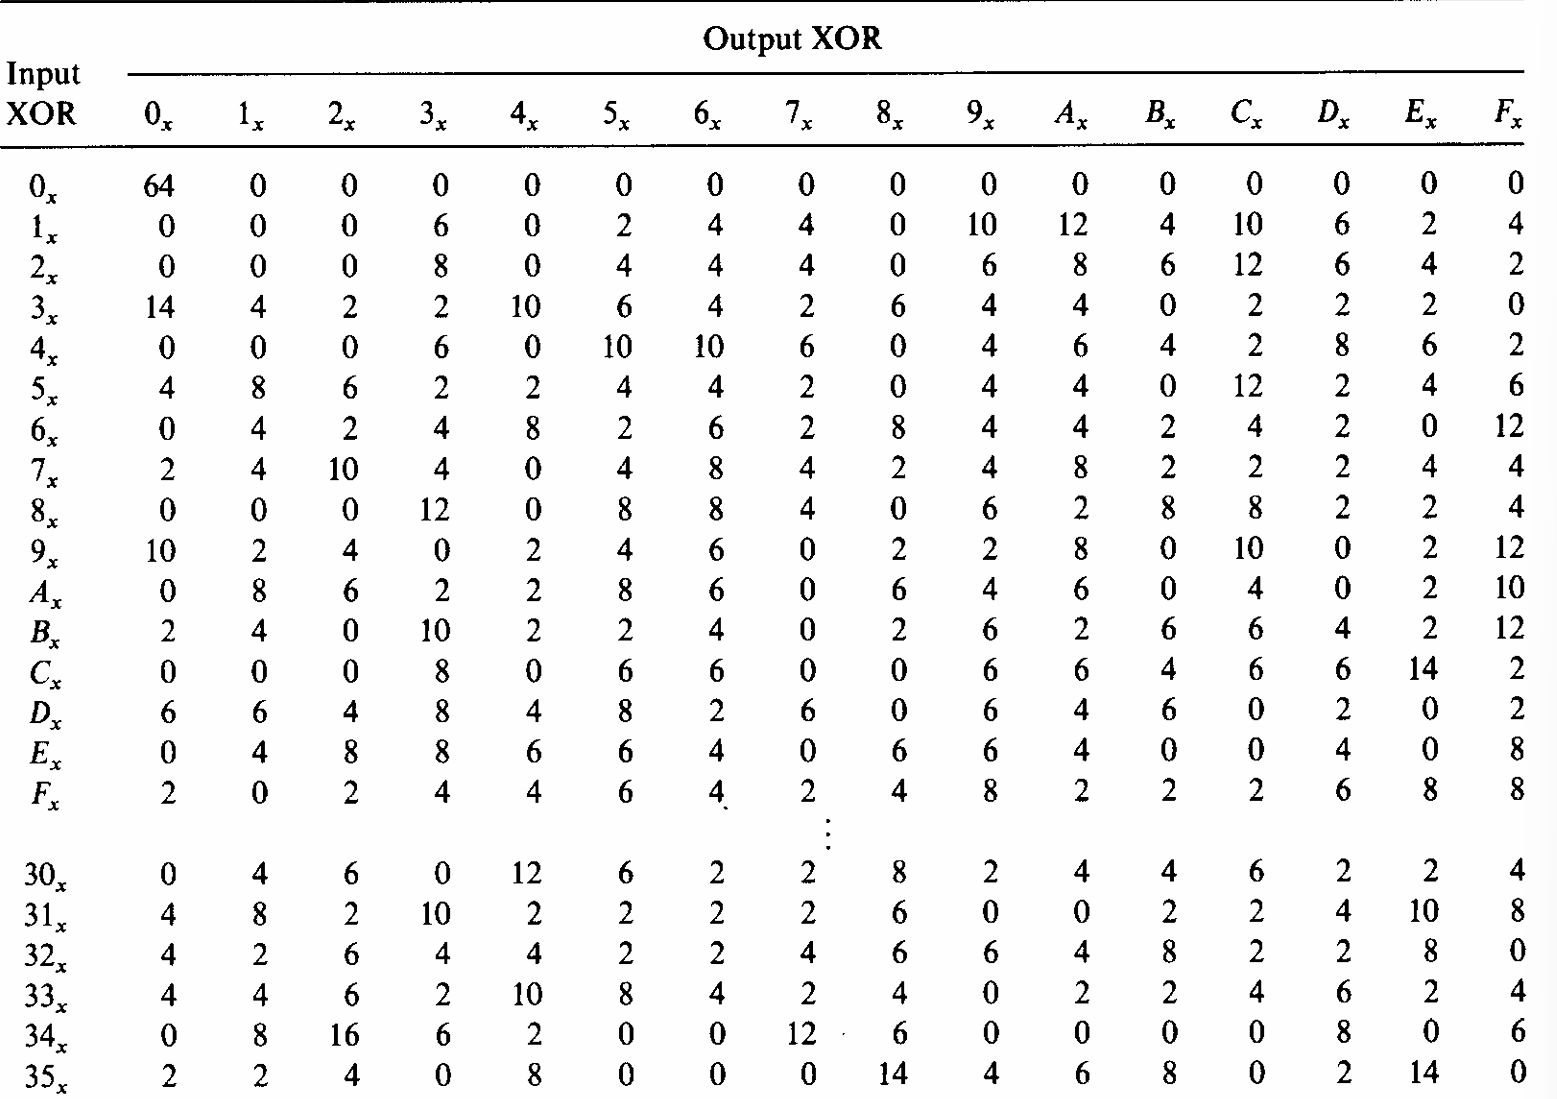
\includegraphics[width=0.75\linewidth]{Sbox-1 table}
\caption{\label{fig:form5} S-box 1 table for $\alpha = \text{Input XOR}$, $\beta = \text{Output XOR}$ [3, p16]}
\end{figure}

Using only two plaintexts with fixed difference value and two encryptions, I can get a fixed output difference value.
With the above two difference values, I can get a set of possible pairs of \verb|XOR|$ed$ texts, and then I can find all possible
round keys according to the set of possible pairs of \verb|XOR|$ed$ texts and the two input plaintexts. Because apply \verb|XOR|
operations to two plaintexts $x$ and $x1$ with two keys $k$ and $k2$ will result the \verb|XOR|$ed$ texts, I can then get
the possible keys using the \verb|XOR| operations between the plaintexts and \verb|XOR|$ed$ texts by \verb|xor_trans|. By keeping
trying new plaintexts and then generating corresponding \verb|XOR|$ed$ texts set, I can keep narrowing down the range
of possible keys.

\begin{alltt}
  \HOLTokenTurnstile{} \HOLSymConst{\HOLTokenForall{}}(\HOLBoundVar{x} :\ensuremath{\alpha} \HOLTyOp{word}) (\ensuremath{\HOLBoundVar{x}\sp{\prime{}}} :\ensuremath{\alpha} \HOLTyOp{word}) (\HOLBoundVar{k} :\ensuremath{\alpha} \HOLTyOp{word}).
     \HOLBoundVar{x} \HOLSymConst{\HOLTokenEor{}} \HOLBoundVar{k} \HOLSymConst{=} \ensuremath{\HOLBoundVar{x}\sp{\prime{}}} \HOLSymConst{\HOLTokenImp{}} \HOLBoundVar{x} \HOLSymConst{\HOLTokenEor{}} \ensuremath{\HOLBoundVar{x}\sp{\prime{}}} \HOLSymConst{=} \HOLBoundVar{k}\hfill{[xor_trans]}
\end{alltt}

\subsection{Differential Cryptanalysis implementation}
However, each S-box has $2^6$ possible input $XORs$, $2^4$ possible output $XORs$ and there are $2^6$ pairs of plaintexts
with each possible input \verb|XOR|. For a total of 8 S-boxes, the tables that records the possible \verb|XOR|$ed$ texts are too
complex and the implementation of the real attack in HOL4 is not necessary for now. As a result, I implement the sets of \verb|XOR|$ed$
plaintexts for S-box one and for the overall round function in a round. I prove the basic correctness of the S-box one
set, and verify properties related to them.

First of all, I proved that a set of pairs of words of length 6 with fixed \verb|XOR| value is bijective to the set of
words with length 6. They are also proved to have the same cardinality, it can verify the property of pairs XOR distribution
table of
the S-box. It states that each line in a pairs XOR distribution table contains 64 possible pairs, means each particular
input \verb|XOR| has 64 possible pairs of word 6 inputs. I define
sets of pairs of word 6 that one half has the fixed difference value of $X$ with the other half. As the set of
the universal set of word 6 has the cardinality of $2^6\;=\;64$, I can then prove the pairs sets also has the cardinality
of $2^6\;=\;64$.

\begin{alltt}
  \HOLTokenTurnstile{} \HOLSymConst{\HOLTokenForall{}}(\HOLBoundVar{X} :\HOLTyOp{word6}). \HOLConst{AllpairXor} \HOLBoundVar{X} \HOLSymConst{=} \HOLTokenLeftbrace{}(\ensuremath{\HOLBoundVar{x}\sb{\mathrm{1}}}\HOLSymConst{,}\ensuremath{\HOLBoundVar{x}\sb{\mathrm{2}}}) \HOLTokenBar{} \ensuremath{\HOLBoundVar{x}\sb{\mathrm{1}}} \HOLSymConst{\HOLTokenEor{}} \ensuremath{\HOLBoundVar{x}\sb{\mathrm{2}}} \HOLSymConst{=} \HOLBoundVar{X}\HOLTokenRightbrace{}\hfill{[AllpairXor_def]}
\end{alltt}

\begin{alltt}
  \HOLTokenTurnstile{} \HOLSymConst{\HOLTokenForall{}}(\HOLBoundVar{X} :\HOLTyOp{word6}). \HOLConst{BIJ} (\HOLConst{trans2} \HOLBoundVar{X}) \ensuremath{{\cal{U}}}(:\HOLTyOp{word6}) (\HOLConst{AllpairXor} \HOLBoundVar{X})\hfill{[BIJ_XORL]}
\end{alltt}

\begin{alltt}
  \HOLTokenTurnstile{} \HOLSymConst{\HOLTokenForall{}}(\HOLBoundVar{X} :\HOLTyOp{word6}).
     \HOLConst{CARD} (\HOLConst{AllpairXor} \HOLBoundVar{X}) \HOLSymConst{=} (((\HOLNumLit{2} :\HOLTyOp{num}) \HOLSymConst{\HOLTokenExp{}} (\HOLNumLit{6} :\HOLTyOp{num})) :\HOLTyOp{num})\hfill{[AllpairXor_card]}
\end{alltt}

By defining two mapping functions, one just returns a half in pair given the pair, to map the universal set of word 6 to
the pairs set. The other function take the $X$ difference value as input, and return a pair that one half is any word6 message,
the other half is the word6 message that differs from the first by $X$. It maps the functions in another order. By using
the \verb|BIJ_IFF_INV| theorem, I can convert the goal to four separate sub-goals about mapping elements between functions.
All sub-goals can be proved directly by applying the definitions of sets and mapping functions to the goal.

\begin{alltt}
  \HOLTokenTurnstile{} \HOLSymConst{\HOLTokenForall{}}(\ensuremath{\HOLBoundVar{x}\sb{\mathrm{1}}} :\HOLTyOp{word6}) (\ensuremath{\HOLBoundVar{x}\sb{\mathrm{2}}} :\HOLTyOp{word6}). \HOLConst{trans1} (\ensuremath{\HOLBoundVar{x}\sb{\mathrm{1}}}\HOLSymConst{,}\ensuremath{\HOLBoundVar{x}\sb{\mathrm{2}}}) \HOLSymConst{=} \ensuremath{\HOLBoundVar{x}\sb{\mathrm{1}}}\hfill{[trans1_def]}
\end{alltt}

\begin{alltt}
  \HOLTokenTurnstile{} \HOLSymConst{\HOLTokenForall{}}(\HOLBoundVar{X} :\HOLTyOp{word6}) (\HOLBoundVar{x} :\HOLTyOp{word6}). \HOLConst{trans2} \HOLBoundVar{X} \HOLBoundVar{x} \HOLSymConst{=} (\HOLBoundVar{x}\HOLSymConst{,}\HOLBoundVar{x} \HOLSymConst{\HOLTokenEor{}} \HOLBoundVar{X})\hfill{[trans2_def]}
\end{alltt}

Next, I implement the definition of ``X may cause Y with probability p by an S-box''[4] in HOL4. It means for all
pairs of \verb|XOR|$ed$ texts that the input \verb|XOR| is $X$ and the output \verb|XOR| after going through a S-box is Y, the number
of these pairs is p percentage out of all possible pairs of \verb|XOR|$ed$ texts that the input \verb|XOR| is X.
These \verb|XOR|$ed$ texts are in word 6 as the inputs of S-box and the input \verb|XOR| is X means the pairs of
texts is differ by X. The overall pairs of \verb|XOR|$ed$ texts that the input \verb|XOR| is X can then be form as the set of pairs
of words of length 6 with fixed \verb|XOR| value and the number of them is the cardinality of this set. As proved above,
the set can then be converted to universal set of word 6 with the same functionality.

Then for the implementation of sets of possible pairs of \verb|XOR|$ed$ texts with both input \verb|XOR| X and output \verb|XOR| Y,
I find it can also convert to sets of single 6-bit texts that takes the $X$, $Y$ and the $S-box$ as input that has the
same functionality. It is also because one half can be expressed using the other half and $X$.

\begin{alltt}
  \HOLTokenTurnstile{} \HOLSymConst{\HOLTokenForall{}}(\HOLBoundVar{X} :\HOLTyOp{word6}) (\HOLBoundVar{Y} :\HOLTyOp{word4}) (\HOLBoundVar{Sb} :\HOLTyOp{sbox}).
     \HOLConst{word6_set1} \HOLBoundVar{X} \HOLBoundVar{Y} \HOLBoundVar{Sb} \HOLSymConst{=} \HOLTokenLeftbrace{}\HOLBoundVar{x} \HOLTokenBar{} \HOLBoundVar{Sb} \HOLBoundVar{x} \HOLSymConst{\HOLTokenEor{}} \HOLBoundVar{Sb} (\HOLBoundVar{x} \HOLSymConst{\HOLTokenEor{}} \HOLBoundVar{X}) \HOLSymConst{=} \HOLBoundVar{Y}\HOLTokenRightbrace{}\hfill{[word6_set1_def]}
\end{alltt}

\begin{alltt}
  \HOLTokenTurnstile{} \HOLSymConst{\HOLTokenForall{}}(\HOLBoundVar{X} :\HOLTyOp{word6}) (\HOLBoundVar{Y} :\HOLTyOp{word4}) (\HOLBoundVar{Sb} :\HOLTyOp{sbox}).
     \HOLConst{word6_set2} \HOLBoundVar{X} \HOLBoundVar{Y} \HOLBoundVar{Sb} \HOLSymConst{=}
     \HOLTokenLeftbrace{}(\ensuremath{\HOLBoundVar{x}\sb{\mathrm{1}}}\HOLSymConst{,}\ensuremath{\HOLBoundVar{x}\sb{\mathrm{2}}}) \HOLTokenBar{} \ensuremath{\HOLBoundVar{x}\sb{\mathrm{1}}} \HOLSymConst{\HOLTokenEor{}} \ensuremath{\HOLBoundVar{x}\sb{\mathrm{2}}} \HOLSymConst{=} \HOLBoundVar{X} \HOLSymConst{\HOLTokenConj{}} \HOLBoundVar{Sb} \ensuremath{\HOLBoundVar{x}\sb{\mathrm{1}}} \HOLSymConst{\HOLTokenEor{}} \HOLBoundVar{Sb} \ensuremath{\HOLBoundVar{x}\sb{\mathrm{2}}} \HOLSymConst{=} \HOLBoundVar{Y}\HOLTokenRightbrace{}\hfill{[word6_set2_def]}
\end{alltt}

The verifications are exactly the same, I define the two mapping functions, one maps a pair of words to only a half, the
other one use a single 6-bit message to produce the other half by exclusive-or operation with input \verb|XOR|. Then by rewriting
with \verb|BIJ_IFF_INV|, \verb|FINITE_BIJ_CARD| and applying the definitions to the goal, BIJ relation and same cardinality
verifications are done.

\begin{alltt}
  \HOLTokenTurnstile{} \HOLSymConst{\HOLTokenForall{}}(\HOLBoundVar{X} :\HOLTyOp{word6}) (\HOLBoundVar{Y} :\HOLTyOp{word4}) (\HOLBoundVar{Sb} :\HOLTyOp{sbox}).
     \HOLConst{BIJ} (\HOLConst{word6_trans1} \HOLBoundVar{X}) (\HOLConst{word6_set1} \HOLBoundVar{X} \HOLBoundVar{Y} \HOLBoundVar{Sb})
       (\HOLConst{word6_set2} \HOLBoundVar{X} \HOLBoundVar{Y} \HOLBoundVar{Sb})\hfill{[BIJ_pairXcY]}
\end{alltt}

\begin{alltt}
  \HOLTokenTurnstile{} \HOLSymConst{\HOLTokenForall{}}(\HOLBoundVar{X} :\HOLTyOp{word6}) (\HOLBoundVar{Y} :\HOLTyOp{word4}) (\HOLBoundVar{Sb} :\HOLTyOp{sbox}).
     \HOLConst{CARD} (\HOLConst{word6_set1} \HOLBoundVar{X} \HOLBoundVar{Y} \HOLBoundVar{Sb}) \HOLSymConst{=} \HOLConst{CARD} (\HOLConst{word6_set2} \HOLBoundVar{X} \HOLBoundVar{Y} \HOLBoundVar{Sb})\hfill{[pairXcY_card]}
\end{alltt}

\subsection{Differential Cryptanalysis using Probability Space}
The target set and the universal set is implemented, I can then implement probability space with the sample space,
set of events and probability of event to help produce
the probability. In HOL4, the theorem \verb|prob_uniform_on_finite_set| states the prerequisites for a measure space
to become a probability space which is suited for my usage. A measure space needs to meet the prerequisites that the measure
space is a finite set and is not empty, the measurable set is the
power set of measure space . Moreover, for each set in the power set, the measure of each set needs to be equal to the
cardinality of each set divided by the cardinality of sample space.
The space, measurable sets, measure of measure space are exactly the same with the components of probability
space - sample space, set of events and the probability of event once measure space is proved also to be a probability space.
From the prerequisites, we can obviously see that, the universal set word 6 can be the sample space.
The sets of single 6-bit texts with input \verb|XOR| X, output \verb|XOR| Y and chosen S-boxes are the events that belong to the
pow set of the universal set.
The required probability p of X may cause Y can then be generated as the probability of events in that probability space.

\begin{alltt}
  \HOLTokenTurnstile{} \HOLSymConst{\HOLTokenForall{}}(\HOLBoundVar{p} :\ensuremath{\alpha} \HOLTyOp{m_space}).
     \HOLConst{FINITE} (\HOLConst{p_space} \HOLBoundVar{p}) \HOLSymConst{\HOLTokenConj{}} \HOLConst{p_space} \HOLBoundVar{p} \HOLSymConst{\HOLTokenNotEqual{}} (\HOLSymConst{\HOLTokenEmpty{}} :\ensuremath{\alpha} \HOLTokenMap{} \HOLTyOp{bool}) \HOLSymConst{\HOLTokenConj{}}
     \HOLConst{events} \HOLBoundVar{p} \HOLSymConst{=} \HOLConst{POW} (\HOLConst{p_space} \HOLBoundVar{p}) \HOLSymConst{\HOLTokenConj{}}
     (\HOLSymConst{\HOLTokenForall{}}(\HOLBoundVar{s} :\ensuremath{\alpha} \HOLTokenMap{} \HOLTyOp{bool}).
        \HOLBoundVar{s} \HOLSymConst{\HOLTokenIn{}} \HOLConst{events} \HOLBoundVar{p} \HOLSymConst{\HOLTokenImp{}}
        \HOLConst{prob} \HOLBoundVar{p} \HOLBoundVar{s} \HOLSymConst{=}
        ((((\HOLSymConst{\&}\HOLConst{CARD} \HOLBoundVar{s}) :\HOLTyOp{extreal}) \HOLSymConst{/} ((\HOLSymConst{\&}\HOLConst{CARD} (\HOLConst{p_space} \HOLBoundVar{p})) :\HOLTyOp{extreal}))
           :\HOLTyOp{extreal})) \HOLSymConst{\HOLTokenImp{}}
     \HOLConst{prob_space} \HOLBoundVar{p}\hfill{[prob_uniform_on_finite_set]}
\end{alltt}

To proving \verb|prob_uniform_on_finite_set| given the prerequisites, I first convert the sample space,
set of events and probability of event back
to the space, measurable sets and measure by their definitions to match with the input $p$ as a measure space. Then I
verify that the measure space is not empty as it is finite.
Then using the theorem \verb|prob_on_finite_set|, I can
expand the goal to three sub-goals. Once I proved that a measure space $p$ is positive, additive and the probability
for the space is 1, then $p$ is a probability space.

\begin{alltt}
  \HOLTokenTurnstile{} \HOLSymConst{\HOLTokenForall{}}(\HOLBoundVar{p} :\ensuremath{\alpha} \HOLTyOp{m_space}).
     \HOLConst{FINITE} (\HOLConst{m_space} \HOLBoundVar{p}) \HOLSymConst{\HOLTokenConj{}} \HOLConst{measurable_sets} \HOLBoundVar{p} \HOLSymConst{=} \HOLConst{POW} (\HOLConst{m_space} \HOLBoundVar{p}) \HOLSymConst{\HOLTokenImp{}}
     (\HOLConst{prob_space} \HOLBoundVar{p} \HOLSymConst{\HOLTokenEquiv{}}
      \HOLConst{positive} \HOLBoundVar{p} \HOLSymConst{\HOLTokenConj{}} \HOLConst{prob} \HOLBoundVar{p} (\HOLConst{p_space} \HOLBoundVar{p}) \HOLSymConst{=} (\HOLNumLit{1} :\HOLTyOp{extreal}) \HOLSymConst{\HOLTokenConj{}}
      \HOLConst{additive} \HOLBoundVar{p})\hfill{[prob_on_finite_set]}
\end{alltt}

The positivity of a measure space means the measure is 0 on empty set and greater than 0 for all other sets. By combining
with the last prerequisite and definition of positivity, the sub-goal changes to prove the cardinality of empty set divided
by the cardinality of space is 0 and the cardinality of all other sets divided by the cardinality of space is greater
or equal to 0. This can be easily done by shown the cardinality of empty set is 0, all sets has cardinality $>=0$ and
the space is not empty. However, as calculations in measure space are in type \verb|extreal| in HOL4, so built-in theorems
in \verb|extreal_Theory| are needed to help complete the proof. These theorems help do calculations, operations and
comparisons for these numbers like the \verb|extreal_lt_eq| theorem

\begin{alltt}
  \HOLTokenTurnstile{} \HOLSymConst{\HOLTokenForall{}}(\HOLBoundVar{x} :\HOLTyOp{real}) (\HOLBoundVar{y} :\HOLTyOp{real}). \HOLConst{Normal} \HOLBoundVar{x} \HOLSymConst{\HOLTokenLt{}} \HOLConst{Normal} \HOLBoundVar{y} \HOLSymConst{\HOLTokenEquiv{}} \HOLBoundVar{x} \HOLSymConst{\HOLTokenLt{}} \HOLBoundVar{y}
\end{alltt}

Then to show the probability for the space is 1, it is to show the cardinality of space out of the cardinality of itself
is one. It is also quite obviously, but as the cardinality is in the type of \verb|extreal| which contains positive and
negative infinite, I need to ensure the cardinality of the space is not 0, positive infinite and negative infinite. It
can be directly proved by the assumptions that space is a finite and non-empty set. But \verb|extreal| definition is also needed
to expand the operation $\&$ in the goal \verb|extreal_of_num_def| to do the comparisons.

\begin{alltt}
  \HOLTokenTurnstile{} \HOLSymConst{\HOLTokenForall{}}(\HOLBoundVar{n} :\HOLTyOp{num}). ((\HOLSymConst{\&}\HOLBoundVar{n}) :\HOLTyOp{extreal}) \HOLSymConst{=} \HOLConst{Normal} ((\HOLSymConst{\&}\HOLBoundVar{n}) :\HOLTyOp{real})
\end{alltt}

At last, I need to prove the additivity of the measure space. It means for any two disjoint sets, if both of them
and their union belong to the power set of the space, the addition of the measures of the two sets is equivalent
to the measure of their union set. By applying the assumption, I want to solve the following goal:

\begin{multline*}
\frac{\text{\&CARD} \; (s \cup t)}{\text{\&CARD} \; (m\_space \, p)} = \frac{\text{\&CARD} \; s}{\text{\&CARD} \; (m\_space \, p)} + \frac{\text{\&CARD} \; t}{\text{\&CARD} \; (m\_space \, p)}
\end{multline*}

I then want to show the cardinality of the union is equal to the sum of the two sets. By applying the tacitic
\verb|MATCH_MP_TAC| introduced earlier, I need to show the two sets are finite and disjoint from each other. The disjoint
goal is directly proved. Use the theorem that for sets belong to the power set of a finite set, these sets are the subsets
of that set, I can then prove these subsets are also finite. After some simple conversions, and use the theorem \verb|div_add|
with all the necessary prerequisites, the additivity is proved.

\begin{alltt}
  \HOLTokenTurnstile{} \HOLSymConst{\HOLTokenForall{}}\HOLBoundVar{set} \HOLBoundVar{e}. \HOLBoundVar{e} \HOLSymConst{\HOLTokenIn{}} \HOLConst{POW} \HOLBoundVar{set} \HOLSymConst{\HOLTokenEquiv{}} \HOLBoundVar{e} \HOLSymConst{\HOLTokenSubset{}} \HOLBoundVar{set}\hfill{[IN_POW]}
\end{alltt}

\begin{alltt}
  \HOLTokenTurnstile{} \HOLSymConst{\HOLTokenForall{}}\HOLBoundVar{s} \HOLBoundVar{t}. \HOLConst{FINITE} \HOLBoundVar{s} \HOLSymConst{\HOLTokenConj{}} \HOLBoundVar{t} \HOLSymConst{\HOLTokenSubset{}} \HOLBoundVar{s} \HOLSymConst{\HOLTokenImp{}} \HOLConst{FINITE} \HOLBoundVar{t}\hfill{[SUBSET_FINITE_I]}
\end{alltt}

Overall, the measure space with the given prerequisites is also a probability space.

Now, I can build my measure spaces about differential cryptanalysis and the sets containing \verb|XOR|$ed$ texts. I can then use
the implementations to generate the probability once I proved that they are probability spaces. I need to create a measure space
that the measurable sets contains the sets of single 6-bit texts that generated by input $X$, $Y$ and the selected $S-box$.
The space of the measure space is defined as the universal set of word in length 6 which has probability of 1 ,
measurable sets are the power set of the universal set of word6. The measure is the cardinality of sets in measurable sets
out of the cardinality of space which is $2^6$. I need then prove the defined measurable space \verb|word6p| is
a probability space by proving \verb|word6p| meets all the prerequisites mentioned above.

\begin{alltt}
  \HOLTokenTurnstile{} \HOLConst{word6p} \HOLSymConst{=}
   (\ensuremath{{\cal{U}}}(:\HOLTyOp{word6})\HOLSymConst{,}\HOLConst{POW} \ensuremath{{\cal{U}}}(:\HOLTyOp{word6})\HOLSymConst{,}
    (\HOLTokenLambda{}(\HOLBoundVar{s} :\HOLTyOp{word6} \HOLTokenMap{} \HOLTyOp{bool}).
         ((((\HOLSymConst{\&}\HOLConst{CARD} \HOLBoundVar{s}) :\HOLTyOp{extreal}) \HOLSymConst{/}
           ((\HOLSymConst{\&}(((\HOLNumLit{2} :\HOLTyOp{num}) \HOLSymConst{\HOLTokenExp{}} (\HOLNumLit{6} :\HOLTyOp{num})) :\HOLTyOp{num})) :\HOLTyOp{extreal}))
            :\HOLTyOp{extreal})))\hfill{[word6p_def]}
\end{alltt}

In theorem \verb|prob_space_word6p|, the use of \verb|MATCH_MP_TAC| converts the goal to all the prerequisites mentioned in the
verified theorem \verb|prob_uniform_on_finite_set|. Then the proof is quite simple, I convert sample space, set of events
and the probability of event function back to the space, measurable sets and measure of measure space function to use the
definitions of them. I can then easily prove the space in \verb|word6p| is finite and non-empty, the measurable sets are the power
set of the space by the definition of \verb|word6p|.  The measure is calculated by the cardinality of sets in power set
out of the space can also be proved by showing the space has the cardinality of $2^6$.

\begin{alltt}
  \HOLTokenTurnstile{} \HOLConst{prob_space} \HOLConst{word6p}\hfill{[prob_space_word6p]}
\end{alltt}

I can then get the probability of my required set using the probability of event. I define a
function \verb|XcauseY_def| to generate the event with input \verb|XOR|, output \verb|XOR| and S-box as inputs, get the
probability of such events and return the probability. I do some tests on the generated envet
and the probability, using the examples provided in [4]. If I choose the input difference of two texts through
S-box 1 to be $0x34w$ and the corresponding output difference of S-box to be $0x4w$, the possible \verb|XOR|$ed$ texts are
$0x13w$ and $0x27w$. It also means sets of possible pairs of \verb|XOR|$ed$ texts are
${(0x13w\,,\, 0x27w)\;,\;(0x27w\,,\,0x13w)}$
according to the conversion discussed earlier which also has the cardinality of 2.

\begin{alltt}
  \HOLTokenTurnstile{} \HOLSymConst{\HOLTokenForall{}}(\HOLBoundVar{X} :\HOLTyOp{word6}) (\HOLBoundVar{Y} :\ensuremath{\alpha} \HOLTyOp{word}) (\HOLBoundVar{Sb} :\HOLTyOp{word6} \HOLTokenMap{} \ensuremath{\alpha} \HOLTyOp{word}).
     \HOLConst{XcauseY} \HOLBoundVar{X} \HOLBoundVar{Y} \HOLBoundVar{Sb} \HOLSymConst{=} \HOLConst{prob} \HOLConst{word6p} \HOLTokenLeftbrace{}\HOLBoundVar{x} \HOLTokenBar{} \HOLBoundVar{Sb} \HOLBoundVar{x} \HOLSymConst{\HOLTokenEor{}} \HOLBoundVar{Sb} (\HOLBoundVar{x} \HOLSymConst{\HOLTokenEor{}} \HOLBoundVar{X}) \HOLSymConst{=} \HOLBoundVar{Y}\HOLTokenRightbrace{}\hfill{[XcauseY_def]}
\end{alltt}

\begin{alltt}
  \HOLTokenTurnstile{} \HOLTokenLeftbrace{}\HOLBoundVar{x} \HOLTokenBar{} \HOLConst{S1} \HOLBoundVar{x} \HOLSymConst{\HOLTokenEor{}} \HOLConst{S1} (\HOLBoundVar{x} \HOLSymConst{\HOLTokenEor{}} (52w :word6)) \HOLSymConst{=} (4w :word4)\HOLTokenRightbrace{} \HOLSymConst{=}
   \HOLTokenLeftbrace{}(19w :word6); (39w :word6)\HOLTokenRightbrace{}\hfill{[word6p_convert]}
\end{alltt}

To prove two sets are the same, I can prove all elements in one set are also in the other by \verb|EXTENSION|
in HOL4. I can then convert the goal to the form with a function and a universally quantified input
variable $x$. It means for a general variable x, I apply function S-box 1 $S1$ to x and to $x\,\oplus\, 0x34w$.
The \verb|XOR| difference of the two outputs equals to $0x4w$ if and only if variable x is either $0x13w$ or $0x27w$.

\begin{alltt}
  \HOLTokenTurnstile{} \HOLFreeVar{s} \HOLSymConst{=} \HOLFreeVar{t} \HOLSymConst{\HOLTokenEquiv{}} \HOLSymConst{\HOLTokenForall{}}\HOLBoundVar{x}. \HOLBoundVar{x} \HOLSymConst{\HOLTokenIn{}} \HOLFreeVar{s} \HOLSymConst{\HOLTokenEquiv{}} \HOLBoundVar{x} \HOLSymConst{\HOLTokenIn{}} \HOLFreeVar{t}\hfill{[EXTENSION]}
\end{alltt}

\begin{equation*}
\begin{split}
   \forall x.\, &\left( \lambda x.\, S1(x) \oplus S1(x \oplus 52\text{w}) = 4\text{w} \Leftrightarrow \right. \\
   & \left. x = 19\text{w} \vee x = 39\text{w} \right)\; x
\end{split}
\end{equation*}

Then by using a variable i in the type of number to represent the x, I can do the method of exhaustion. By testing
all the 64 possible words in length 6, I can complete the proof as all words except $0x13w$ and $0x27w$ do not
satisfy the property on both sides. Only these two words can satisfy ``iff'' goal.

\begin{equation*}
\begin{split}
    (w = n2w \; i) \land (i < 64)
\end{split}
\end{equation*}

$n2w$ means converting a number to word, and there is also $w2n$ operation means converting in the other direction.

I can consequently prove the probability of this event is $2/64$. By showing this event has two elements, and the cardinality
is 2 using the above theorem, I can complete the verification with simple rewrites of definitions.

\begin{alltt}
  \HOLTokenTurnstile{} \HOLConst{XcauseYp} (52w :word6) (4w :word4) \HOLConst{S1}
     (((\HOLNumLit{2} :\HOLTyOp{extreal}) \HOLSymConst{/} (\HOLNumLit{64} :\HOLTyOp{extreal})) :\HOLTyOp{extreal})\hfill{[XcauseYp_test]}
\end{alltt}

Moreover, I can implement the events and probabilities for ``X may cause Y with probability p by the F function''[4] in
differential cryptanalysis. It is almost the same for the earlier one, but change single S-box to the overall round
function including the expansion operation, \verb|XOR| operation with round key, S-boxes operation and $P$ permutation. The
input $X$ is the difference of two 32-bit plaintexts at the beginning of round and the output difference $Y$ should
be the difference between ciphertexts after $P$ permutation. The F function can be seen in Figure~\ref{fig:form7}
The transformed pair of texts go through the S-boxes
should be in the form of:

\begin{equation*}
\begin{split}
(E(x1)\,\oplus\, k\;,\; E(x2)\,\oplus\, k)= (x1'\;,\;x2')
\end{split}
\end{equation*}

\begin{figure}
\centering
\includegraphics[width=0.75\linewidth]{F function}
\caption{\label{fig:form7} Round function of DES [4,p10]}
\end{figure}

The difference between x1 and x2 is the input \verb|XOR| $X$. After the above two halves going through the S-box, and applying the
$P$ permutation, the difference between the results is output \verb|XOR| $Y$. The result halves are also differed by a fixed
value. It is because x1 and x2 are differed by $X$, $E(x1)$ and $E(x2)$ are differed by $E(X)$ using
the \verb|xor_E| theorem I proved. Then by the theorem \verb|xor_twice|, the difference between $x1'$ and $x2'$ is $E(X)$. As a
result, $x2'$ can be represented by $x1'$ using their difference.
The fraction is based on all possible input pairs encrypted by all possible round keys.
By combining with these two halves have length of 48, the sample
space should be the universal set of pairs of all word48, and then can be converted to the universal set of word48 as $x2'$
can also be represented using $x1'$.  The related proof is shown in \verb|xor_Com|.

\begin{alltt}
  \HOLTokenTurnstile{} \HOLSymConst{\HOLTokenForall{}}(\ensuremath{\HOLBoundVar{x}\sb{\mathrm{1}}} :\HOLTyOp{word32}) (\ensuremath{\HOLBoundVar{x}\sb{\mathrm{2}}} :\HOLTyOp{word32}) (\HOLBoundVar{k} :\HOLTyOp{word48}) (\HOLBoundVar{X} :\HOLTyOp{word32}).
     \ensuremath{\HOLBoundVar{x}\sb{\mathrm{1}}} \HOLSymConst{\HOLTokenEor{}} \ensuremath{\HOLBoundVar{x}\sb{\mathrm{2}}} \HOLSymConst{=} \HOLBoundVar{X} \HOLSymConst{\HOLTokenImp{}} (\HOLConst{E} \ensuremath{\HOLBoundVar{x}\sb{\mathrm{1}}} \HOLSymConst{\HOLTokenEor{}} \HOLBoundVar{k}) \HOLSymConst{\HOLTokenEor{}} \HOLConst{E} \ensuremath{\HOLBoundVar{x}\sb{\mathrm{2}}} \HOLSymConst{\HOLTokenEor{}} \HOLBoundVar{k} \HOLSymConst{=} \HOLConst{E} \HOLBoundVar{X}\hfill{[xor_Com]}
\end{alltt}

However, if I want to build the probability space for events of the possible input pairs encrypted by all the possible
subkey values, it is too complex and hard to build. There are total $2^{32}$ possible of inputs pairs before expansion as the pairs
are different by a fix value, and they can produce at most $2^{32}$ expanded inputs pairs. As the word length is 48 now, the sample
space is the subset of all possible the expanded inputs which has the cardinality of at most $2^{32}$. Then I need to encrypt these
expanded inputs pairs with all possible subkey values with length 48, it will results $(2^{32})*(2^{48})$ pairs. It is hard to
determine how many words in length 48 can be generated even known the pairs are differ by a fix value. Moreover, as I cannot ensure
all possible word48 words can be generated by all word32 words after expansion and \verb|XOR| operation, I also cannot ensure the sample
space for each S-box probability space contains all word6 words. As a result, I choose to generate the events for pairs of texts after
the expansion and \verb|XOR| operation with round keys. It has not been proved to be the same as using inputs pairs of round function, but a
simpler and variant version. Using the variant version, I can verify the properties about ``X may cause Y with probability p by the F function'',
to ``X may cause Y with probability p by the S-boxes'' which the X and Y are still the original definitions.
I then verify the correctness towards the variant definitions.

The sample space for the variant version should be the universal set of pairs of all word48, and then can be converted to the universal set of
word48 using the exact same proof steps for word6 sample space.

\begin{alltt}
   \HOLTokenTurnstile{} \HOLSymConst{\HOLTokenForall{}}(\HOLBoundVar{X} :\HOLTyOp{word48}). \HOLConst{BIJ} (\HOLConst{trans48_2} \HOLBoundVar{X}) \ensuremath{{\cal{U}}}(:\HOLTyOp{word48}) (\HOLConst{word48Xor} \HOLBoundVar{X})\hfill{[BIJ_XOR48]}
\end{alltt}

\begin{alltt}
   \HOLTokenTurnstile{} \HOLSymConst{\HOLTokenForall{}}(\HOLBoundVar{X} :\HOLTyOp{word48}).
     \HOLConst{CARD} (\HOLConst{word48Xor} \HOLBoundVar{X}) \HOLSymConst{=} (((\HOLNumLit{2} :\HOLTyOp{num}) \HOLSymConst{\HOLTokenExp{}} (\HOLNumLit{48} :\HOLTyOp{num})) :\HOLTyOp{num})\hfill{[word48Xor_card]}
\end{alltt}

The events should then in the form of:

\begin{equation*}
   Assuming \quad(E(x1)\,\oplus\, k\;,\; E(x2)\,\oplus\, k)= (x1'\;,\;x2')
\end{equation*}

\begin{equation*}
Set: \{(x1', x2') \;|\; x1' \oplus x2' = E(X) \land S(x1') \oplus S(x2')= P^{-1}(Y)\}
\end{equation*}

The implementation in HOL4 can directly use $x1'$ and $x2'$ with $X$ and $P^{-1}(Y)$ as inputs without changing the
functionality. The use of $P^{-1}(Y)$ as input will only change the corresponding event,
and can be treated as omitting one extra step of transferring the $Y$ in definition to $P^{-1}$. It will not affect the
verifications for related
properties, but it is for convenience. Moreover, the event form can also be further simplied with only $x1'$ by expressing
$x2'$ using $x1'$ with the exactly same proof steps for theorem \verb|BIJ_pairXcY| and \verb|pairXcY_card|.

\begin{alltt}
\HOLTokenTurnstile{} \HOLSymConst{\HOLTokenForall{}}(\HOLBoundVar{X} :\HOLTyOp{word32}) (\HOLBoundVar{Y} :\HOLTyOp{word32}).
     \HOLConst{word48_set1} \HOLBoundVar{X} \HOLBoundVar{Y} \HOLSymConst{=}
     \HOLTokenLeftbrace{}\HOLBoundVar{x} \HOLTokenBar{} (\HOLConst{S} \HOLBoundVar{x} :\HOLTyOp{word32}) \HOLSymConst{\HOLTokenEor{}} (\HOLConst{S} (\HOLBoundVar{x} \HOLSymConst{\HOLTokenEor{}} \HOLConst{E} \HOLBoundVar{X}) :\HOLTyOp{word32}) \HOLSymConst{=} \HOLBoundVar{Y}\HOLTokenRightbrace{}\hfill{[word48_set1_def]}
\end{alltt}

\begin{alltt}
\HOLTokenTurnstile{} \HOLSymConst{\HOLTokenForall{}}(\HOLBoundVar{X} :\HOLTyOp{word32}) (\HOLBoundVar{Y} :\HOLTyOp{word32}).
     \HOLConst{word48_set2} \HOLBoundVar{X} \HOLBoundVar{Y} \HOLSymConst{=}
     \HOLTokenLeftbrace{}(\ensuremath{\HOLBoundVar{x}\sb{\mathrm{1}}}\HOLSymConst{,}\ensuremath{\HOLBoundVar{x}\sb{\mathrm{2}}}) \HOLTokenBar{}
      \ensuremath{\HOLBoundVar{x}\sb{\mathrm{1}}} \HOLSymConst{\HOLTokenEor{}} \ensuremath{\HOLBoundVar{x}\sb{\mathrm{2}}} \HOLSymConst{=} \HOLConst{E} \HOLBoundVar{X} \HOLSymConst{\HOLTokenConj{}} (\HOLConst{S} \ensuremath{\HOLBoundVar{x}\sb{\mathrm{1}}} :\HOLTyOp{word32}) \HOLSymConst{\HOLTokenEor{}} (\HOLConst{S} \ensuremath{\HOLBoundVar{x}\sb{\mathrm{2}}} :\HOLTyOp{word32}) \HOLSymConst{=} \HOLBoundVar{Y}\HOLTokenRightbrace{}\hfill{[word48_set2_def]}
\end{alltt}

\begin{alltt}
\HOLTokenTurnstile{} \HOLSymConst{\HOLTokenForall{}}(\HOLBoundVar{X} :\HOLTyOp{word32}) (\HOLBoundVar{Y} :\HOLTyOp{word32}).
     \HOLConst{BIJ} (\HOLConst{word48_trans1} \HOLBoundVar{X}) (\HOLConst{word48_set1} \HOLBoundVar{X} \HOLBoundVar{Y}) (\HOLConst{word48_set2} \HOLBoundVar{X} \HOLBoundVar{Y})\hfill{[BIJ_pairXcYF]}
\end{alltt}

\begin{alltt}
\HOLTokenTurnstile{} \HOLSymConst{\HOLTokenForall{}}(\HOLBoundVar{X} :\HOLTyOp{word32}) (\HOLBoundVar{Y} :\HOLTyOp{word32}).
     \HOLConst{CARD} (\HOLConst{word48_set1} \HOLBoundVar{X} \HOLBoundVar{Y}) \HOLSymConst{=} \HOLConst{CARD} (\HOLConst{word48_set2} \HOLBoundVar{X} \HOLBoundVar{Y})\hfill{[pairXcYF_card]}
\end{alltt}

The measure space can then be implemented and proved as a probability space with the simplified sample space and events.
I can also implement the probability of all possible pairs going through S-boxes with input \verb|XOR| $X$ and output \verb|XOR| Y.
\begin{alltt}
\HOLTokenTurnstile{} \HOLConst{word48p} \HOLSymConst{=}
   (\ensuremath{{\cal{U}}}(:\HOLTyOp{word48})\HOLSymConst{,}\HOLConst{POW} \ensuremath{{\cal{U}}}(:\HOLTyOp{word48})\HOLSymConst{,}
    (\HOLTokenLambda{}(\HOLBoundVar{s} :\HOLTyOp{word48} \HOLTokenMap{} \HOLTyOp{bool}).
         ((((\HOLSymConst{\&}\HOLConst{CARD} \HOLBoundVar{s}) :\HOLTyOp{extreal}) \HOLSymConst{/}
           ((\HOLSymConst{\&}(((\HOLNumLit{2} :\HOLTyOp{num}) \HOLSymConst{\HOLTokenExp{}} (\HOLNumLit{48} :\HOLTyOp{num})) :\HOLTyOp{num})) :\HOLTyOp{extreal}))
            :\HOLTyOp{extreal})))\hfill{[word48p_def]}
\end{alltt}

\begin{alltt}
\HOLTokenTurnstile{} \HOLConst{prob_space} \HOLConst{word48p}\hfill{[prob_space_word48p]}
\end{alltt}

\begin{alltt}
\HOLTokenTurnstile{} \HOLSymConst{\HOLTokenForall{}}(\HOLBoundVar{X} :\HOLTyOp{word32}) (\HOLBoundVar{Y} :\HOLTyOp{word32}).
     \HOLConst{XcauseYF'} \HOLBoundVar{X} \HOLBoundVar{Y} \HOLSymConst{=}
     \HOLConst{prob} \HOLConst{word48p}
       \HOLTokenLeftbrace{}\HOLBoundVar{x} \HOLTokenBar{} (\HOLConst{S} \HOLBoundVar{x} :\HOLTyOp{word32}) \HOLSymConst{\HOLTokenEor{}} (\HOLConst{S} (\HOLBoundVar{x} \HOLSymConst{\HOLTokenEor{}} \HOLConst{E} \HOLBoundVar{X}) :\HOLTyOp{word32}) \HOLSymConst{=} \HOLBoundVar{Y}\HOLTokenRightbrace{}\hfill{[XcauseYF'_def]}
\end{alltt}

\subsection{Differential Cryptanalysis Properties}
Next, I can verify a corollary about the probability partially , it states that
The probability $p$ of $X \rightarrow Y$ by the F function is the product of $P_i$ in
which $X_i \rightarrow Y_i$ by the S-boxes $S_i$ $(i \in \{1, \dots, 8\})$ [4]. From $X_1$ to $X_8$, they concat X that
start with $X_8$ as the 4-bit of X from the lowest 4-bit part and going up, the process is repeated to $X_8$.
Similar to $Y_i$, $Y_i$ from $i=8$ represents the 4th to 1st bits of $Y$ to $i=1$ represent the 32nd to 29th bits.
Using the variant version, the property is transformed that $Y$ is in fact $P^{-1}(Y)$, and F function is now S-boxes.

To start the proof, I first I define two split lists, so that each $X_i$ and $Y_i$ is generated within lists. The two lists
use $E(X)$ and $Y$ as the input. I also define \verb|S_data_def| to match each corresponding $X_i$, $Y_i$ and S-box. S-box $i$
is matched to the $X_i$ and $Y_i$ by using \verb|EL n list| to get the $i$th element in each list.

\begin{alltt}
\HOLTokenTurnstile{} \HOLSymConst{\HOLTokenForall{}}(\HOLBoundVar{Xe} :\HOLTyOp{word48}).
     \HOLConst{splitXF} \HOLBoundVar{Xe} \HOLSymConst{=}
     [(((\HOLNumLit{5} :\HOLTyOp{num}) \HOLSymConst{\HOLTokenExtract{}} (\HOLNumLit{0} :\HOLTyOp{num})) \HOLBoundVar{Xe} :\HOLTyOp{word6});
      (((\HOLNumLit{11} :\HOLTyOp{num}) \HOLSymConst{\HOLTokenExtract{}} (\HOLNumLit{6} :\HOLTyOp{num})) \HOLBoundVar{Xe} :\HOLTyOp{word6});
      (((\HOLNumLit{17} :\HOLTyOp{num}) \HOLSymConst{\HOLTokenExtract{}} (\HOLNumLit{12} :\HOLTyOp{num})) \HOLBoundVar{Xe} :\HOLTyOp{word6});
      (((\HOLNumLit{23} :\HOLTyOp{num}) \HOLSymConst{\HOLTokenExtract{}} (\HOLNumLit{18} :\HOLTyOp{num})) \HOLBoundVar{Xe} :\HOLTyOp{word6});
      (((\HOLNumLit{29} :\HOLTyOp{num}) \HOLSymConst{\HOLTokenExtract{}} (\HOLNumLit{24} :\HOLTyOp{num})) \HOLBoundVar{Xe} :\HOLTyOp{word6});
      (((\HOLNumLit{35} :\HOLTyOp{num}) \HOLSymConst{\HOLTokenExtract{}} (\HOLNumLit{30} :\HOLTyOp{num})) \HOLBoundVar{Xe} :\HOLTyOp{word6});
      (((\HOLNumLit{41} :\HOLTyOp{num}) \HOLSymConst{\HOLTokenExtract{}} (\HOLNumLit{36} :\HOLTyOp{num})) \HOLBoundVar{Xe} :\HOLTyOp{word6});
      (((\HOLNumLit{47} :\HOLTyOp{num}) \HOLSymConst{\HOLTokenExtract{}} (\HOLNumLit{42} :\HOLTyOp{num})) \HOLBoundVar{Xe} :\HOLTyOp{word6})]\hfill{[splitXF_def]}
\end{alltt}

\begin{alltt}
\HOLTokenTurnstile{} \HOLSymConst{\HOLTokenForall{}}(\HOLBoundVar{Ye} :\HOLTyOp{word32}).
     \HOLConst{splitYF} \HOLBoundVar{Ye} \HOLSymConst{=}
     [(((\HOLNumLit{3} :\HOLTyOp{num}) \HOLSymConst{\HOLTokenExtract{}} (\HOLNumLit{0} :\HOLTyOp{num})) \HOLBoundVar{Ye} :\HOLTyOp{word4});
      (((\HOLNumLit{7} :\HOLTyOp{num}) \HOLSymConst{\HOLTokenExtract{}} (\HOLNumLit{4} :\HOLTyOp{num})) \HOLBoundVar{Ye} :\HOLTyOp{word4});
      (((\HOLNumLit{11} :\HOLTyOp{num}) \HOLSymConst{\HOLTokenExtract{}} (\HOLNumLit{8} :\HOLTyOp{num})) \HOLBoundVar{Ye} :\HOLTyOp{word4});
      (((\HOLNumLit{15} :\HOLTyOp{num}) \HOLSymConst{\HOLTokenExtract{}} (\HOLNumLit{12} :\HOLTyOp{num})) \HOLBoundVar{Ye} :\HOLTyOp{word4});
      (((\HOLNumLit{19} :\HOLTyOp{num}) \HOLSymConst{\HOLTokenExtract{}} (\HOLNumLit{16} :\HOLTyOp{num})) \HOLBoundVar{Ye} :\HOLTyOp{word4});
      (((\HOLNumLit{23} :\HOLTyOp{num}) \HOLSymConst{\HOLTokenExtract{}} (\HOLNumLit{20} :\HOLTyOp{num})) \HOLBoundVar{Ye} :\HOLTyOp{word4});
      (((\HOLNumLit{27} :\HOLTyOp{num}) \HOLSymConst{\HOLTokenExtract{}} (\HOLNumLit{24} :\HOLTyOp{num})) \HOLBoundVar{Ye} :\HOLTyOp{word4});
      (((\HOLNumLit{31} :\HOLTyOp{num}) \HOLSymConst{\HOLTokenExtract{}} (\HOLNumLit{28} :\HOLTyOp{num})) \HOLBoundVar{Ye} :\HOLTyOp{word4})]\hfill{[splitYF_def]}
\end{alltt}

\begin{alltt}
\HOLTokenTurnstile{} \HOLConst{S_data} \HOLSymConst{=}
   [\HOLConst{S8_data}; \HOLConst{S7_data}; \HOLConst{S6_data}; \HOLConst{S5_data}; \HOLConst{S4_data}; \HOLConst{S3_data};
    \HOLConst{S2_data}; \HOLConst{S1_data}]\hfill{[S_data_def]}
\end{alltt}

I can then build my theorem in HOL4 with theorem \verb|XcauseYFp_eq|. It state that for the probability of event for S-boxes using $X$ and
$Y$, it is equal to the product of probability of event for single S-box with corresponding \verb|X_i|, \verb|Y_i| and \verb|S-box i|. It
use \verb|EXTREAL_PROD_IMAGE| to achieve repeatedly production for a lambda function with \verb|extreal| type for $8$ times here.

\begin{alltt}
\HOLTokenTurnstile{} \HOLSymConst{\HOLTokenForall{}}(\HOLBoundVar{X} :\HOLTyOp{word32}) (\HOLBoundVar{Y} :\HOLTyOp{word32}).
     (\HOLFreeVar{Xe} :\HOLTyOp{word48}) \HOLSymConst{=} \HOLConst{E} \HOLBoundVar{X} \HOLSymConst{\HOLTokenConj{}} (\HOLFreeVar{Xl} :\HOLTyOp{word6} \HOLTyOp{list}) \HOLSymConst{=} \HOLConst{splitXF} \HOLFreeVar{Xe} \HOLSymConst{\HOLTokenConj{}}
     (\HOLFreeVar{Yl} :\HOLTyOp{word4} \HOLTyOp{list}) \HOLSymConst{=} \HOLConst{splitYF} \HOLBoundVar{Y} \HOLSymConst{\HOLTokenImp{}}
     \HOLConst{XcauseYF'} \HOLBoundVar{X} \HOLBoundVar{Y} \HOLSymConst{=}
     \HOLSymConst{\HOLTokenPI{}}
       (\HOLTokenLambda{}(\HOLBoundVar{i} :\HOLTyOp{num}).
            \HOLConst{XcauseY} (\HOLConst{EL} \HOLBoundVar{i} \HOLFreeVar{Xl}) (\HOLConst{EL} \HOLBoundVar{i} \HOLFreeVar{Yl}) (\HOLConst{SBox} (\HOLConst{EL} \HOLBoundVar{i} \HOLConst{S_data})))
       (\HOLConst{count} (\HOLNumLit{8} :\HOLTyOp{num}))\hfill{[XcauseYFp_eq]}
\end{alltt}

Although it is a convenient way to define the goal, I need repeat steps of proof to separate each probability of event out
for further analysis. I can use \verb|EXTREAL_PROD_IMAGE_COUNT_SUC| to keep separating the $i$th probability of events out from the
\verb|EXTREAL_PROD_IMAGE| function that product $(i-1)$ probability of events.

\begin{alltt}
\HOLTokenTurnstile{} \HOLSymConst{\HOLTokenForall{}}(\HOLBoundVar{f} :\HOLTyOp{num} \HOLTokenMap{} \HOLTyOp{extreal}) (\HOLBoundVar{n} :\HOLTyOp{num}).
     \HOLSymConst{\HOLTokenPI{}} \HOLBoundVar{f} (\HOLConst{count1} \HOLBoundVar{n}) \HOLSymConst{=} ((\HOLSymConst{\HOLTokenPI{}} \HOLBoundVar{f} (\HOLConst{count} \HOLBoundVar{n}) \HOLSymConst{\HOLTokenProd{}} \HOLBoundVar{f} \HOLBoundVar{n}) :\HOLTyOp{extreal})\hfill{[EXTREAL_PROD_IMAGE_COUNT_SUC]}
\end{alltt}

By converting them to normal product form, I use the definitions
of both sides to expand them. The probabilities of events on both sides can now coverted in the form of the cardinality of event divide by
the cardinality of sample space. The cardinality of sample space is directly number of $2^{48}$ and $2^{6}$.
Now, it means that I need to prove the number of \verb|XOR|$ed$ texts $x$ with inputs texts differ by $X$ and outputs text after going through whole
S-boxes are differed by $Y$ is equal to
the product of the number of \verb|XOR|$ed$ texts $x_i$ with inputs texts differ by $X_i$ and outputs text differ by $Y_i$ after going through single
S-box $i$. There are a total of 8 $x_i$ from $(i=1)$ to $(i=8)$
Then I use a support theorem
\verb|CARD_eqF| to convert the cardinality of event for full S-boxes to the cardinality of another set \verb|(XpairF X Y)|, as they are proved
to be bijection and thus have the same cardinality. By using another theorem \verb|F_convert|, I can keep transforming the set \verb|(XpairF X Y)|
to be the cross of all eight events for a single S-box. I can then use the property of cross operation that the cardinality of cross function is equal
to the product of the cardinality of I can then use the property of cross operation that the cardinality of cross function is equal
to the product of the cardinality of the cardinalities of the individual sets. This property has been built in HOL4
called \verb|CARD_CROSS|. My goal can now become like below, which only left the \verb|extreal| type conversions and calculations.

\begin{align*}
   & \frac{\&CARD(s1 \times s2 \times s3 \times s4 \times s5 \times s6 \times s7 \times s8)}{2^{48}} \\
  = \; & \frac{\&CARD(s1)}{64} \cdot \frac{\&CARD(s2)}{64} \cdot \frac{\&CARD(s3)}{64} \cdot \frac{\&CARD(s4)}{64} \cdot \\
     & \frac{\&CARD(s5)}{64} \cdot \frac{\&CARD(s6)}{64} \cdot \frac{\&CARD(s7)}{64} \cdot \frac{\&CARD(s8)}{64}
\end{align*}

\begin{alltt}
\HOLTokenTurnstile{} \HOLSymConst{\HOLTokenForall{}}\HOLBoundVar{P} \HOLBoundVar{Q}. \HOLConst{FINITE} \HOLBoundVar{P} \HOLSymConst{\HOLTokenConj{}} \HOLConst{FINITE} \HOLBoundVar{Q} \HOLSymConst{\HOLTokenImp{}} \HOLConst{CARD} (\HOLBoundVar{P} \HOLSymConst{\ensuremath{\times}} \HOLBoundVar{Q}) \HOLSymConst{=} \HOLConst{CARD} \HOLBoundVar{P} \HOLSymConst{\HOLTokenProd{}} \HOLConst{CARD} \HOLBoundVar{Q}\hfill{[CARD_CROSS]}
\end{alltt}

First of all, I add \verb|NORMAL| using \verb|extreal_of_num_def| to enable calculations in \verb|extreal| mentioned before
and convert all the divisions to multiplication by $(-1)$ using \verb|div_eq_mul_linv|. At last, by converting all numbers within a
\verb|NORMAL| operation, I can calculate numbers in type of \verb|real| now. The goal is finished by automatically calculation.

\begin{alltt}
\HOLTokenTurnstile{} \HOLSymConst{\HOLTokenForall{}}(\HOLBoundVar{x} :\HOLTyOp{extreal}) (\HOLBoundVar{y} :\HOLTyOp{extreal}).
     \HOLBoundVar{x} \HOLSymConst{\HOLTokenNotEqual{}} \HOLSymConst{\ensuremath{+\infty}} \HOLSymConst{\HOLTokenConj{}} \HOLBoundVar{x} \HOLSymConst{\HOLTokenNotEqual{}} \HOLSymConst{\ensuremath{-\infty}} \HOLSymConst{\HOLTokenConj{}} (\HOLNumLit{0} :\HOLTyOp{extreal}) \HOLSymConst{\HOLTokenLt{}} \HOLBoundVar{y} \HOLSymConst{\HOLTokenImp{}}
     ((\HOLBoundVar{x} \HOLSymConst{/} \HOLBoundVar{y}) :\HOLTyOp{extreal}) \HOLSymConst{=} ((\HOLBoundVar{y}\HOLSymConst{\HOLTokenInverse{}} \HOLSymConst{\HOLTokenProd{}} \HOLBoundVar{x}) :\HOLTyOp{extreal})\hfill{[div_eq_mul_linv]}
\end{alltt}

\begin{alltt}
\HOLTokenTurnstile{} \HOLSymConst{\HOLTokenForall{}}(\HOLBoundVar{x} :\HOLTyOp{real}). \HOLBoundVar{x} \HOLSymConst{\HOLTokenNotEqual{}} (\HOLNumLit{0} :\HOLTyOp{real}) \HOLSymConst{\HOLTokenImp{}} (\HOLConst{Normal} \HOLBoundVar{x})\HOLSymConst{\HOLTokenInverse{}} \HOLSymConst{=} \HOLConst{Normal} \HOLBoundVar{x}\HOLSymConst{\HOLTokenInverse{}}\hfill{[extreal_inv_eq]}
\end{alltt}

\begin{alltt}
\HOLTokenTurnstile{} \HOLSymConst{\HOLTokenForall{}}(\HOLBoundVar{x} :\HOLTyOp{real}) (\HOLBoundVar{y} :\HOLTyOp{real}).
     ((\HOLConst{Normal} \HOLBoundVar{x} \HOLSymConst{\HOLTokenProd{}} \HOLConst{Normal} \HOLBoundVar{y}) :\HOLTyOp{extreal}) \HOLSymConst{=} \HOLConst{Normal} ((\HOLBoundVar{x} \HOLSymConst{\HOLTokenProd{}} \HOLBoundVar{y}) :\HOLTyOp{real})\hfill{[extreal_mul_eq]}
\end{alltt}

It is now time to prove the first support theorem \verb|F_convert|. \verb|(XpairF X Y)| set is implemented
with the inputs are input \verb|XOR| and output \verb|XOR| of F function. It is a set of tuples of 8 with $x_i$ $(i \in \{1, \dots, 8\})$.
Each $x_i$ can be considered as the \verb|XOR|$ed$ text that has fixed difference with another text by $X_i$, apply to S-box $i$
and outputs texts have difference of $Y_i$. The $X_i$ and $Y_i$ are produced by the inputs $X$ and $Y$ as described above.

\begin{alltt}
\HOLTokenTurnstile{} \HOLSymConst{\HOLTokenForall{}}\HOLBoundVar{X} \HOLBoundVar{Y}.
     \HOLConst{XpairF} \HOLBoundVar{X} \HOLBoundVar{Y} \HOLSymConst{=}
     \HOLTokenLeftbrace{}(\ensuremath{\HOLBoundVar{x}\sb{\mathrm{8}}}\HOLSymConst{,}\ensuremath{\HOLBoundVar{x}\sb{\mathrm{7}}}\HOLSymConst{,}\ensuremath{\HOLBoundVar{x}\sb{\mathrm{6}}}\HOLSymConst{,}\ensuremath{\HOLBoundVar{x}\sb{\mathrm{5}}}\HOLSymConst{,}\ensuremath{\HOLBoundVar{x}\sb{\mathrm{4}}}\HOLSymConst{,}\ensuremath{\HOLBoundVar{x}\sb{\mathrm{3}}}\HOLSymConst{,}\ensuremath{\HOLBoundVar{x}\sb{\mathrm{2}}}\HOLSymConst{,}\ensuremath{\HOLBoundVar{x}\sb{\mathrm{1}}}) \HOLTokenBar{}
      \HOLConst{S8} \ensuremath{\HOLBoundVar{x}\sb{\mathrm{1}}} \HOLSymConst{\HOLTokenEor{}} \HOLConst{S8} (\ensuremath{\HOLBoundVar{x}\sb{\mathrm{1}}} \HOLSymConst{\HOLTokenEor{}} (\HOLNumLit{5} \HOLSymConst{\HOLTokenExtract{}} \HOLNumLit{0}) (\HOLConst{E} \HOLBoundVar{X})) \HOLSymConst{=} (\HOLNumLit{3} \HOLSymConst{\HOLTokenExtract{}} \HOLNumLit{0}) \HOLBoundVar{Y} \HOLSymConst{\HOLTokenConj{}}
      \HOLConst{S7} \ensuremath{\HOLBoundVar{x}\sb{\mathrm{2}}} \HOLSymConst{\HOLTokenEor{}} \HOLConst{S7} (\ensuremath{\HOLBoundVar{x}\sb{\mathrm{2}}} \HOLSymConst{\HOLTokenEor{}} (\HOLNumLit{11} \HOLSymConst{\HOLTokenExtract{}} \HOLNumLit{6}) (\HOLConst{E} \HOLBoundVar{X})) \HOLSymConst{=} (\HOLNumLit{7} \HOLSymConst{\HOLTokenExtract{}} \HOLNumLit{4}) \HOLBoundVar{Y} \HOLSymConst{\HOLTokenConj{}}
      \HOLConst{S6} \ensuremath{\HOLBoundVar{x}\sb{\mathrm{3}}} \HOLSymConst{\HOLTokenEor{}} \HOLConst{S6} (\ensuremath{\HOLBoundVar{x}\sb{\mathrm{3}}} \HOLSymConst{\HOLTokenEor{}} (\HOLNumLit{17} \HOLSymConst{\HOLTokenExtract{}} \HOLNumLit{12}) (\HOLConst{E} \HOLBoundVar{X})) \HOLSymConst{=} (\HOLNumLit{11} \HOLSymConst{\HOLTokenExtract{}} \HOLNumLit{8}) \HOLBoundVar{Y} \HOLSymConst{\HOLTokenConj{}}
      \HOLConst{S5} \ensuremath{\HOLBoundVar{x}\sb{\mathrm{4}}} \HOLSymConst{\HOLTokenEor{}} \HOLConst{S5} (\ensuremath{\HOLBoundVar{x}\sb{\mathrm{4}}} \HOLSymConst{\HOLTokenEor{}} (\HOLNumLit{23} \HOLSymConst{\HOLTokenExtract{}} \HOLNumLit{18}) (\HOLConst{E} \HOLBoundVar{X})) \HOLSymConst{=} (\HOLNumLit{15} \HOLSymConst{\HOLTokenExtract{}} \HOLNumLit{12}) \HOLBoundVar{Y} \HOLSymConst{\HOLTokenConj{}}
      \HOLConst{S4} \ensuremath{\HOLBoundVar{x}\sb{\mathrm{5}}} \HOLSymConst{\HOLTokenEor{}} \HOLConst{S4} (\ensuremath{\HOLBoundVar{x}\sb{\mathrm{5}}} \HOLSymConst{\HOLTokenEor{}} (\HOLNumLit{29} \HOLSymConst{\HOLTokenExtract{}} \HOLNumLit{24}) (\HOLConst{E} \HOLBoundVar{X})) \HOLSymConst{=} (\HOLNumLit{19} \HOLSymConst{\HOLTokenExtract{}} \HOLNumLit{16}) \HOLBoundVar{Y} \HOLSymConst{\HOLTokenConj{}}
      \HOLConst{S3} \ensuremath{\HOLBoundVar{x}\sb{\mathrm{6}}} \HOLSymConst{\HOLTokenEor{}} \HOLConst{S3} (\ensuremath{\HOLBoundVar{x}\sb{\mathrm{6}}} \HOLSymConst{\HOLTokenEor{}} (\HOLNumLit{35} \HOLSymConst{\HOLTokenExtract{}} \HOLNumLit{30}) (\HOLConst{E} \HOLBoundVar{X})) \HOLSymConst{=} (\HOLNumLit{23} \HOLSymConst{\HOLTokenExtract{}} \HOLNumLit{20}) \HOLBoundVar{Y} \HOLSymConst{\HOLTokenConj{}}
      \HOLConst{S2} \ensuremath{\HOLBoundVar{x}\sb{\mathrm{7}}} \HOLSymConst{\HOLTokenEor{}} \HOLConst{S2} (\ensuremath{\HOLBoundVar{x}\sb{\mathrm{7}}} \HOLSymConst{\HOLTokenEor{}} (\HOLNumLit{41} \HOLSymConst{\HOLTokenExtract{}} \HOLNumLit{36}) (\HOLConst{E} \HOLBoundVar{X})) \HOLSymConst{=} (\HOLNumLit{27} \HOLSymConst{\HOLTokenExtract{}} \HOLNumLit{24}) \HOLBoundVar{Y} \HOLSymConst{\HOLTokenConj{}}
      \HOLConst{S1} \ensuremath{\HOLBoundVar{x}\sb{\mathrm{8}}} \HOLSymConst{\HOLTokenEor{}} \HOLConst{S1} (\ensuremath{\HOLBoundVar{x}\sb{\mathrm{8}}} \HOLSymConst{\HOLTokenEor{}} (\HOLNumLit{47} \HOLSymConst{\HOLTokenExtract{}} \HOLNumLit{42}) (\HOLConst{E} \HOLBoundVar{X})) \HOLSymConst{=} (\HOLNumLit{31} \HOLSymConst{\HOLTokenExtract{}} \HOLNumLit{28}) \HOLBoundVar{Y}\HOLTokenRightbrace{}\hfill{[XpairF_def]}
\end{alltt}

Each element in the tuple can be treated as separated out to produce a set of $x_i$, and the cross product of the
eight sets which are the events of single S-box is equal to the set of tuples. The theorem is implemented and proved
in \verb|F_convert|.

\begin{alltt}
\HOLTokenTurnstile{} \HOLSymConst{\HOLTokenForall{}}\HOLBoundVar{X} \HOLBoundVar{Y}.
     \HOLConst{XpairF} \HOLBoundVar{X} \HOLBoundVar{Y} \HOLSymConst{=}
     \HOLTokenLeftbrace{}\HOLBoundVar{x} \HOLTokenBar{} \HOLConst{S1} \HOLBoundVar{x} \HOLSymConst{\HOLTokenEor{}} \HOLConst{S1} (\HOLBoundVar{x} \HOLSymConst{\HOLTokenEor{}} (\HOLNumLit{47} \HOLSymConst{\HOLTokenExtract{}} \HOLNumLit{42}) (\HOLConst{E} \HOLBoundVar{X})) \HOLSymConst{=} (\HOLNumLit{31} \HOLSymConst{\HOLTokenExtract{}} \HOLNumLit{28}) \HOLBoundVar{Y}\HOLTokenRightbrace{} \HOLSymConst{\ensuremath{\times}}
     \HOLTokenLeftbrace{}\HOLBoundVar{x} \HOLTokenBar{} \HOLConst{S2} \HOLBoundVar{x} \HOLSymConst{\HOLTokenEor{}} \HOLConst{S2} (\HOLBoundVar{x} \HOLSymConst{\HOLTokenEor{}} (\HOLNumLit{41} \HOLSymConst{\HOLTokenExtract{}} \HOLNumLit{36}) (\HOLConst{E} \HOLBoundVar{X})) \HOLSymConst{=} (\HOLNumLit{27} \HOLSymConst{\HOLTokenExtract{}} \HOLNumLit{24}) \HOLBoundVar{Y}\HOLTokenRightbrace{} \HOLSymConst{\ensuremath{\times}}
     \HOLTokenLeftbrace{}\HOLBoundVar{x} \HOLTokenBar{} \HOLConst{S3} \HOLBoundVar{x} \HOLSymConst{\HOLTokenEor{}} \HOLConst{S3} (\HOLBoundVar{x} \HOLSymConst{\HOLTokenEor{}} (\HOLNumLit{35} \HOLSymConst{\HOLTokenExtract{}} \HOLNumLit{30}) (\HOLConst{E} \HOLBoundVar{X})) \HOLSymConst{=} (\HOLNumLit{23} \HOLSymConst{\HOLTokenExtract{}} \HOLNumLit{20}) \HOLBoundVar{Y}\HOLTokenRightbrace{} \HOLSymConst{\ensuremath{\times}}
     \HOLTokenLeftbrace{}\HOLBoundVar{x} \HOLTokenBar{} \HOLConst{S4} \HOLBoundVar{x} \HOLSymConst{\HOLTokenEor{}} \HOLConst{S4} (\HOLBoundVar{x} \HOLSymConst{\HOLTokenEor{}} (\HOLNumLit{29} \HOLSymConst{\HOLTokenExtract{}} \HOLNumLit{24}) (\HOLConst{E} \HOLBoundVar{X})) \HOLSymConst{=} (\HOLNumLit{19} \HOLSymConst{\HOLTokenExtract{}} \HOLNumLit{16}) \HOLBoundVar{Y}\HOLTokenRightbrace{} \HOLSymConst{\ensuremath{\times}}
     \HOLTokenLeftbrace{}\HOLBoundVar{x} \HOLTokenBar{} \HOLConst{S5} \HOLBoundVar{x} \HOLSymConst{\HOLTokenEor{}} \HOLConst{S5} (\HOLBoundVar{x} \HOLSymConst{\HOLTokenEor{}} (\HOLNumLit{23} \HOLSymConst{\HOLTokenExtract{}} \HOLNumLit{18}) (\HOLConst{E} \HOLBoundVar{X})) \HOLSymConst{=} (\HOLNumLit{15} \HOLSymConst{\HOLTokenExtract{}} \HOLNumLit{12}) \HOLBoundVar{Y}\HOLTokenRightbrace{} \HOLSymConst{\ensuremath{\times}}
     \HOLTokenLeftbrace{}\HOLBoundVar{x} \HOLTokenBar{} \HOLConst{S6} \HOLBoundVar{x} \HOLSymConst{\HOLTokenEor{}} \HOLConst{S6} (\HOLBoundVar{x} \HOLSymConst{\HOLTokenEor{}} (\HOLNumLit{17} \HOLSymConst{\HOLTokenExtract{}} \HOLNumLit{12}) (\HOLConst{E} \HOLBoundVar{X})) \HOLSymConst{=} (\HOLNumLit{11} \HOLSymConst{\HOLTokenExtract{}} \HOLNumLit{8}) \HOLBoundVar{Y}\HOLTokenRightbrace{} \HOLSymConst{\ensuremath{\times}}
     \HOLTokenLeftbrace{}\HOLBoundVar{x} \HOLTokenBar{} \HOLConst{S7} \HOLBoundVar{x} \HOLSymConst{\HOLTokenEor{}} \HOLConst{S7} (\HOLBoundVar{x} \HOLSymConst{\HOLTokenEor{}} (\HOLNumLit{11} \HOLSymConst{\HOLTokenExtract{}} \HOLNumLit{6}) (\HOLConst{E} \HOLBoundVar{X})) \HOLSymConst{=} (\HOLNumLit{7} \HOLSymConst{\HOLTokenExtract{}} \HOLNumLit{4}) \HOLBoundVar{Y}\HOLTokenRightbrace{} \HOLSymConst{\ensuremath{\times}}
     \HOLTokenLeftbrace{}\HOLBoundVar{x} \HOLTokenBar{} \HOLConst{S8} \HOLBoundVar{x} \HOLSymConst{\HOLTokenEor{}} \HOLConst{S8} (\HOLBoundVar{x} \HOLSymConst{\HOLTokenEor{}} (\HOLNumLit{5} \HOLSymConst{\HOLTokenExtract{}} \HOLNumLit{0}) (\HOLConst{E} \HOLBoundVar{X})) \HOLSymConst{=} (\HOLNumLit{3} \HOLSymConst{\HOLTokenExtract{}} \HOLNumLit{0}) \HOLBoundVar{Y}\HOLTokenRightbrace{}
\end{alltt}

By expanding the definition of \verb|(XpairF X Y)| and use theorem \verb|EXTENSION| mentioned before, I now need to prove
each element in one set is also in another. It means each element should satisfy the properties of both sets.
measurable sets. By applying \verb|GSYM| to theorem \verb|PAIR|, I can use \verb|PAIR| in the reverse direction. After
applying \verb|PAIR| to each element in the tuple, I can represent each element $x_i$ using the tuple. Each $x_i$ is
represented by the \verb|FST| and \verb|SND| operations to the tuple. The ``iff'' goal is now the same on both sides, but
each term on both sides is linked by $\land$ in different order. I can now use an useful tactic \verb|WORD_DECIDE_TAC| to
complete the proof. It is a tactic implemented for \verb|wordsTheory|, it contains many basic rewriting rules and also
rewriting rules specific to deal with \verb|words| theorems. By using it, I can directly finish the proof by the
commutation property of $\land$ operations without finding the specific theorems in HOL4.

\begin{alltt}
\HOLTokenTurnstile{} \HOLSymConst{\HOLTokenForall{}}(\HOLBoundVar{x} :\ensuremath{\alpha} \HOLTokenProd{} \ensuremath{\beta}). (\HOLConst{FST} \HOLBoundVar{x}\HOLSymConst{,}\HOLConst{SND} \HOLBoundVar{x}) \HOLSymConst{=} \HOLBoundVar{x}\hfill{[PAIR]}
\end{alltt}

For the proof for the second support theorem \verb|CARD_eqF|, I prove \verb|(XpairF X Y)| sets' cardinality is
equal to the cardinality of events with possible \verb|XOR| texts of 48-bit going through the whole S-boxes function. Once I
proved these two sets are bijection to each other, I can get they have the same cardinality using \verb|FINITE_BIJ_CARD| and
the same process introduced earlier.

\begin{alltt}
\HOLTokenTurnstile{} \HOLSymConst{\HOLTokenForall{}}(\HOLBoundVar{X} :\HOLTyOp{word32}) (\HOLBoundVar{Y} :\HOLTyOp{word32}).
     \HOLConst{CARD} \HOLTokenLeftbrace{}\HOLBoundVar{x} \HOLTokenBar{} (\HOLConst{S} \HOLBoundVar{x} :\HOLTyOp{word32}) \HOLSymConst{\HOLTokenEor{}} (\HOLConst{S} (\HOLBoundVar{x} \HOLSymConst{\HOLTokenEor{}} \HOLConst{E} \HOLBoundVar{X}) :\HOLTyOp{word32}) \HOLSymConst{=} \HOLBoundVar{Y}\HOLTokenRightbrace{} \HOLSymConst{=}
     \HOLConst{CARD} (\HOLConst{XpairF} \HOLBoundVar{X} \HOLBoundVar{Y})\hfill{[CARD_eqF]}
\end{alltt}

I then require to define two mapping functions to prove the bijection relation. \verb|CARD_eqF| represents set of
tuples that each element in it is $x_i$, and event defined in theorem \verb|XcauseYF'_def| is set that each element is $x$
in \verb|word48|. Consequently, one mapping function takes a tuple of 8 as input and returns a word in length 48 by concatenating
all of $x_i$ in the tuple from 1 to 8. The other mapping function works in the other direction, it extracts to 8 words of length
6, each selects the $(6 \cdot n + 5) \;><\; (6 \cdot n)$ part of $x$, where $0 \leq n \leq 7$ and form them as a tuple.

\begin{alltt}
\HOLTokenTurnstile{} \HOLSymConst{\HOLTokenForall{}}\ensuremath{\HOLBoundVar{x}\sb{\mathrm{1}}} \ensuremath{\HOLBoundVar{x}\sb{\mathrm{2}}} \ensuremath{\HOLBoundVar{x}\sb{\mathrm{3}}} \ensuremath{\HOLBoundVar{x}\sb{\mathrm{4}}} \ensuremath{\HOLBoundVar{x}\sb{\mathrm{5}}} \ensuremath{\HOLBoundVar{x}\sb{\mathrm{6}}} \ensuremath{\HOLBoundVar{x}\sb{\mathrm{7}}} \ensuremath{\HOLBoundVar{x}\sb{\mathrm{8}}}.
     \HOLConst{transF1} (\ensuremath{\HOLBoundVar{x}\sb{\mathrm{1}}}\HOLSymConst{,}\ensuremath{\HOLBoundVar{x}\sb{\mathrm{2}}}\HOLSymConst{,}\ensuremath{\HOLBoundVar{x}\sb{\mathrm{3}}}\HOLSymConst{,}\ensuremath{\HOLBoundVar{x}\sb{\mathrm{4}}}\HOLSymConst{,}\ensuremath{\HOLBoundVar{x}\sb{\mathrm{5}}}\HOLSymConst{,}\ensuremath{\HOLBoundVar{x}\sb{\mathrm{6}}}\HOLSymConst{,}\ensuremath{\HOLBoundVar{x}\sb{\mathrm{7}}}\HOLSymConst{,}\ensuremath{\HOLBoundVar{x}\sb{\mathrm{8}}}) \HOLSymConst{=}
     \ensuremath{\HOLBoundVar{x}\sb{\mathrm{1}}} \HOLSymConst{@@} \ensuremath{\HOLBoundVar{x}\sb{\mathrm{2}}} \HOLSymConst{@@} \ensuremath{\HOLBoundVar{x}\sb{\mathrm{3}}} \HOLSymConst{@@} \ensuremath{\HOLBoundVar{x}\sb{\mathrm{4}}} \HOLSymConst{@@} \ensuremath{\HOLBoundVar{x}\sb{\mathrm{5}}} \HOLSymConst{@@} \ensuremath{\HOLBoundVar{x}\sb{\mathrm{6}}} \HOLSymConst{@@} \ensuremath{\HOLBoundVar{x}\sb{\mathrm{7}}} \HOLSymConst{@@} \ensuremath{\HOLBoundVar{x}\sb{\mathrm{8}}}\hfill{[transF1_def]}
\end{alltt}

\begin{alltt}
\HOLTokenTurnstile{} \HOLSymConst{\HOLTokenForall{}}\HOLBoundVar{x}. \HOLConst{transF2} \HOLBoundVar{x} \HOLSymConst{=}
       ((\HOLNumLit{47} \HOLSymConst{\HOLTokenExtract{}} \HOLNumLit{42}) \HOLBoundVar{x}\HOLSymConst{,}(\HOLNumLit{41} \HOLSymConst{\HOLTokenExtract{}} \HOLNumLit{36}) \HOLBoundVar{x}\HOLSymConst{,}(\HOLNumLit{35} \HOLSymConst{\HOLTokenExtract{}} \HOLNumLit{30}) \HOLBoundVar{x}\HOLSymConst{,}(\HOLNumLit{29} \HOLSymConst{\HOLTokenExtract{}} \HOLNumLit{24}) \HOLBoundVar{x}\HOLSymConst{,}
        (\HOLNumLit{23} \HOLSymConst{\HOLTokenExtract{}} \HOLNumLit{18}) \HOLBoundVar{x}\HOLSymConst{,}(\HOLNumLit{17} \HOLSymConst{\HOLTokenExtract{}} \HOLNumLit{12}) \HOLBoundVar{x}\HOLSymConst{,}(\HOLNumLit{11} \HOLSymConst{\HOLTokenExtract{}} \HOLNumLit{6}) \HOLBoundVar{x}\HOLSymConst{,}(\HOLNumLit{5} \HOLSymConst{\HOLTokenExtract{}} \HOLNumLit{0}) \HOLBoundVar{x})\hfill{[transF2_def]}
\end{alltt}

As usual, \verb|BIJ_IFF_INV| is used to divide the goal to 4 sub-goals. The first one is to prove for $x$, each extracted part or $x$
has the same property as the corresponding $x_i$. After rewriting with definitions, it means each extracted part will cause the same
$Y_i$ given inputs difference $X_i$. The proof is easy by using the definition of the whole S-boxes function
\verb|S_def|. The corresponding bits defined in \verb|S_def| is defined by the same property of single S-box, so it automatically gives me
the required property. The only action required is use the powerful \verb|WORD_DECIDE_TAC| to extract the required part in \verb|S_def| out.

\begin{alltt}
\HOLTokenTurnstile{} \HOLSymConst{\HOLTokenForall{}}(\HOLBoundVar{X} :\HOLTyOp{word32}) (\HOLBoundVar{Y} :\HOLTyOp{word32}).
     \HOLConst{BIJ} \HOLConst{transF2}
       \HOLTokenLeftbrace{}\HOLBoundVar{x} \HOLTokenBar{} (\HOLConst{S} \HOLBoundVar{x} :\HOLTyOp{word32}) \HOLSymConst{\HOLTokenEor{}} (\HOLConst{S} (\HOLBoundVar{x} \HOLSymConst{\HOLTokenEor{}} \HOLConst{E} \HOLBoundVar{X}) :\HOLTyOp{word32}) \HOLSymConst{=} \HOLBoundVar{Y}\HOLTokenRightbrace{}
       (\HOLConst{XpairF} \HOLBoundVar{X} \HOLBoundVar{Y})\hfill{[BIJ_F]}
\end{alltt}

\begin{alltt}
\HOLTokenTurnstile{} \HOLSymConst{\HOLTokenForall{}}\HOLBoundVar{w}. \HOLConst{S} \HOLBoundVar{w} \HOLSymConst{=}
       \HOLConst{concat_word_list}
         [\HOLConst{S8} ((\HOLNumLit{5} \HOLSymConst{\HOLTokenExtract{}} \HOLNumLit{0}) \HOLBoundVar{w}); \HOLConst{S7} ((\HOLNumLit{11} \HOLSymConst{\HOLTokenExtract{}} \HOLNumLit{6}) \HOLBoundVar{w}); \HOLConst{S6} ((\HOLNumLit{17} \HOLSymConst{\HOLTokenExtract{}} \HOLNumLit{12}) \HOLBoundVar{w});
          \HOLConst{S5} ((\HOLNumLit{23} \HOLSymConst{\HOLTokenExtract{}} \HOLNumLit{18}) \HOLBoundVar{w}); \HOLConst{S4} ((\HOLNumLit{29} \HOLSymConst{\HOLTokenExtract{}} \HOLNumLit{24}) \HOLBoundVar{w});
          \HOLConst{S3} ((\HOLNumLit{35} \HOLSymConst{\HOLTokenExtract{}} \HOLNumLit{30}) \HOLBoundVar{w}); \HOLConst{S2} ((\HOLNumLit{41} \HOLSymConst{\HOLTokenExtract{}} \HOLNumLit{36}) \HOLBoundVar{w});
          \HOLConst{S1} ((\HOLNumLit{47} \HOLSymConst{\HOLTokenExtract{}} \HOLNumLit{42}) \HOLBoundVar{w})]\hfill{[S_def]}
\end{alltt}

The second goal that mapping in another way looks complex, it contains many \verb|XOR|,\verb|OR|,\verb|EXTRACT| and \verb|CONCAT|
operations. However, as \verb|EXTRACT| and \verb|CONCAT| can be cancelled out as each word that are concatenate has the same length as
the range asked to be extracted, both in length 6. Moreover, by using the formula that:

\begin{equation*}
(x_1 \parallel x_2 \parallel \dots \parallel x_8) \oplus (x_1' \parallel x_2' \parallel \dots \parallel x_8') = (x_1 \oplus x_1') \parallel (x_2 \oplus x_2') \parallel \dots \parallel (x_8 \oplus x_8')
\end{equation*}

I can convert the simplify the goal and transfer it to the form I want. These can all be done by \verb|WORD_DECIDE_TAC|. Then by the use
of \verb|WORD_w2w_OVER_BITWISE|, I can move all the \verb|w2w| operations that convert the word type to the outermost brackets and gather all the
useful parts together. For now, I can use the assumptions provided to complete the goal

\begin{alltt}
\HOLTokenTurnstile{} (\HOLSymConst{\HOLTokenForall{}}(\HOLBoundVar{v} :\ensuremath{\alpha} \HOLTyOp{word}) (\HOLBoundVar{w} :\ensuremath{\alpha} \HOLTyOp{word}).
      (\HOLConst{w2w} \HOLBoundVar{v} :\ensuremath{\beta} \HOLTyOp{word}) \HOLSymConst{\&\&} (\HOLConst{w2w} \HOLBoundVar{w} :\ensuremath{\beta} \HOLTyOp{word}) \HOLSymConst{=}
      (\HOLConst{w2w} (\HOLBoundVar{v} \HOLSymConst{\&\&} \HOLBoundVar{w}) :\ensuremath{\beta} \HOLTyOp{word})) \HOLSymConst{\HOLTokenConj{}}
   (\HOLSymConst{\HOLTokenForall{}}(\HOLBoundVar{v} :\ensuremath{\alpha} \HOLTyOp{word}) (\HOLBoundVar{w} :\ensuremath{\alpha} \HOLTyOp{word}).
      (\HOLConst{w2w} \HOLBoundVar{v} :\ensuremath{\beta} \HOLTyOp{word}) \HOLSymConst{\HOLTokenOr{}} (\HOLConst{w2w} \HOLBoundVar{w} :\ensuremath{\beta} \HOLTyOp{word}) \HOLSymConst{=}
      (\HOLConst{w2w} (\HOLBoundVar{v} \HOLSymConst{\HOLTokenOr{}} \HOLBoundVar{w}) :\ensuremath{\beta} \HOLTyOp{word})) \HOLSymConst{\HOLTokenConj{}}
   \HOLSymConst{\HOLTokenForall{}}(\HOLBoundVar{v} :\ensuremath{\alpha} \HOLTyOp{word}) (\HOLBoundVar{w} :\ensuremath{\alpha} \HOLTyOp{word}).
     (\HOLConst{w2w} \HOLBoundVar{v} :\ensuremath{\beta} \HOLTyOp{word}) \HOLSymConst{\HOLTokenEor{}} (\HOLConst{w2w} \HOLBoundVar{w} :\ensuremath{\beta} \HOLTyOp{word}) \HOLSymConst{=}
     (\HOLConst{w2w} (\HOLBoundVar{v} \HOLSymConst{\HOLTokenEor{}} \HOLBoundVar{w}) :\ensuremath{\beta} \HOLTyOp{word})\hfill{[WORD_w2w_OVER_BITWISE]}
\end{alltt}

The rest two sub-goals can be directly proved, as they apply both functions together, these two functions can be cancelled out by each other. It will
leave only simple operation conversions that can be done directly by \verb|WORD_DECIDE_TAC|.

As a result, all the support theorems mentioned are proved, and with the help of support theorems, I can conclude the probability of events for
48-bit texts through S-boxes is equal to the product of probabilities of events through single S-box.

For the last part about differential cryptanalysis, I implement a new events for the sample space of word48. It is the sets of round
keys. For a pair of texts after the expansion operation, before \verb|XOR| with round keys(also variant version) and the same input \verb|XOR| value $X$,
the round keys are \verb|XOR| with
both halves. If the results can produce the output \verb|XOR| value that equals to $Y$, these round keys are in the set. The round keys' set
take $X$, $Y$ and a pair of $(x1,x2)$ as
inputs. As the halves can be representeed by each other using $X$ as talked before ,the inputs can be simplified to $X$, $Y$ and $x$. This event has
the property that it has equal probability for the event of \verb|XOR|$ed$ texts $x$ list with the same $X$ and $Y$ [4].

\begin{alltt}
\HOLTokenTurnstile{} \HOLSymConst{\HOLTokenForall{}}(\HOLBoundVar{X} :\HOLTyOp{word32}) (\HOLBoundVar{Y} :\HOLTyOp{word32}) (\HOLBoundVar{x} :\HOLTyOp{word48}).
     \HOLConst{XcauseYFkey} \HOLBoundVar{X} \HOLBoundVar{Y} \HOLBoundVar{x} \HOLSymConst{=}
     (\HOLKeyword{let}
        (\ensuremath{\HOLBoundVar{x}\sp{\prime{}}} :\HOLTyOp{word48}) = \HOLBoundVar{x} \HOLSymConst{\HOLTokenEor{}} \HOLConst{E} \HOLBoundVar{X}
      \HOLKeyword{in}
        \HOLConst{prob} \HOLConst{word48p}
          \HOLTokenLeftbrace{}\HOLBoundVar{k} \HOLTokenBar{} (\HOLConst{S} (\HOLBoundVar{x} \HOLSymConst{\HOLTokenEor{}} \HOLBoundVar{k}) :\HOLTyOp{word32}) \HOLSymConst{\HOLTokenEor{}} (\HOLConst{S} (\ensuremath{\HOLBoundVar{x}\sp{\prime{}}} \HOLSymConst{\HOLTokenEor{}} \HOLBoundVar{k}) :\HOLTyOp{word32}) \HOLSymConst{=} \HOLBoundVar{Y}\HOLTokenRightbrace{})\hfill{[XcauseYFkey_def]}
\end{alltt}

\begin{alltt}
\HOLTokenTurnstile{} \HOLSymConst{\HOLTokenForall{}}(\HOLBoundVar{X} :\HOLTyOp{word32}) (\HOLBoundVar{Y} :\HOLTyOp{word32}) (\HOLBoundVar{x} :\HOLTyOp{word48}).
     \HOLConst{XcauseYFkey} \HOLBoundVar{X} \HOLBoundVar{Y} \HOLBoundVar{x} \HOLSymConst{=} \HOLConst{XcauseYF'} \HOLBoundVar{X} \HOLBoundVar{Y}\hfill{[XcauseYF_convert]}
\end{alltt}

It can also be proved be proving the bijection relation between these two sets. The verification is much simpler.
As round key and \verb|XOR|$ed$ text are differed by the input text of F function after expansion. I can always convert between them using the
\verb|XOR| operation by the input of the round keys' events-the input text of F function after expansion. Then the two mapping functions are just
taking input of the round keys' as input, and convert to each other by \verb|XOR| operation. By using \verb|BIJ_IFF_INV|, and inserting the functions,
bijection proof is done. Using \verb|FINITE_BIJ_CARD|, they are proved to have the same cardinality. Finally, they have the same probability as
their sample spaces are also the same.

\begin{alltt}
\HOLTokenTurnstile{} \HOLSymConst{\HOLTokenForall{}}(\HOLBoundVar{x} :\HOLTyOp{word48}) (\HOLBoundVar{k} :\HOLTyOp{word48}). \HOLConst{transktoxF} \HOLBoundVar{x} \HOLBoundVar{k} \HOLSymConst{=} \HOLBoundVar{k} \HOLSymConst{\HOLTokenEor{}} \HOLBoundVar{x}\hfill{[transktoxF_def]}
\end{alltt}

\begin{alltt}
\HOLTokenTurnstile{} \HOLSymConst{\HOLTokenForall{}}(\HOLBoundVar{x} :\HOLTyOp{word48}) (\ensuremath{\HOLBoundVar{x}\sp{\prime{}}} :\HOLTyOp{word48}). \HOLConst{transxtokF} \HOLBoundVar{x} \ensuremath{\HOLBoundVar{x}\sp{\prime{}}} \HOLSymConst{=} \HOLBoundVar{x} \HOLSymConst{\HOLTokenEor{}} \ensuremath{\HOLBoundVar{x}\sp{\prime{}}}\hfill{[transxtokF_def]}
\end{alltt}

\begin{alltt}
\HOLTokenTurnstile{} \HOLSymConst{\HOLTokenForall{}}(\HOLBoundVar{X} :\HOLTyOp{word32}) (\HOLBoundVar{Y} :\HOLTyOp{word32}) (\HOLBoundVar{x} :\HOLTyOp{word48}).
     \HOLConst{BIJ} (\HOLConst{transktoxF} \HOLBoundVar{x})
       \HOLTokenLeftbrace{}\HOLBoundVar{k} \HOLTokenBar{} (\HOLConst{S} (\HOLBoundVar{k} \HOLSymConst{\HOLTokenEor{}} \HOLBoundVar{x}) :\HOLTyOp{word32}) \HOLSymConst{\HOLTokenEor{}} (\HOLConst{S} (\HOLBoundVar{k} \HOLSymConst{\HOLTokenEor{}} \HOLBoundVar{x} \HOLSymConst{\HOLTokenEor{}} \HOLConst{E} \HOLBoundVar{X}) :\HOLTyOp{word32}) \HOLSymConst{=} \HOLBoundVar{Y}\HOLTokenRightbrace{}
       \HOLTokenLeftbrace{}\HOLBoundVar{x} \HOLTokenBar{} (\HOLConst{S} \HOLBoundVar{x} :\HOLTyOp{word32}) \HOLSymConst{\HOLTokenEor{}} (\HOLConst{S} (\HOLBoundVar{x} \HOLSymConst{\HOLTokenEor{}} \HOLConst{E} \HOLBoundVar{X}) :\HOLTyOp{word32}) \HOLSymConst{=} \HOLBoundVar{Y}\HOLTokenRightbrace{}\hfill{[BIJ_ktox]}
\end{alltt}

\begin{alltt}
\HOLTokenTurnstile{} \HOLSymConst{\HOLTokenForall{}}(\HOLBoundVar{X} :\HOLTyOp{word32}) (\HOLBoundVar{Y} :\HOLTyOp{word32}) (\HOLBoundVar{x} :\HOLTyOp{word48}).
     \HOLConst{CARD}
       \HOLTokenLeftbrace{}\HOLBoundVar{k} \HOLTokenBar{} (\HOLConst{S} (\HOLBoundVar{k} \HOLSymConst{\HOLTokenEor{}} \HOLBoundVar{x}) :\HOLTyOp{word32}) \HOLSymConst{\HOLTokenEor{}} (\HOLConst{S} (\HOLBoundVar{k} \HOLSymConst{\HOLTokenEor{}} \HOLBoundVar{x} \HOLSymConst{\HOLTokenEor{}} \HOLConst{E} \HOLBoundVar{X}) :\HOLTyOp{word32}) \HOLSymConst{=} \HOLBoundVar{Y}\HOLTokenRightbrace{} \HOLSymConst{=}
     \HOLConst{CARD} \HOLTokenLeftbrace{}\HOLBoundVar{x} \HOLTokenBar{} (\HOLConst{S} \HOLBoundVar{x} :\HOLTyOp{word32}) \HOLSymConst{\HOLTokenEor{}} (\HOLConst{S} (\HOLBoundVar{x} \HOLSymConst{\HOLTokenEor{}} \HOLConst{E} \HOLBoundVar{X}) :\HOLTyOp{word32}) \HOLSymConst{=} \HOLBoundVar{Y}\HOLTokenRightbrace{}\hfill{[CARD_kxeq]}
\end{alltt}


\section{RC5 in HOL4}
a

%% APPENDIX
\newcommand{\HOLdesDate}{23 Ottobre 2024}
\newcommand{\HOLdesTime}{10:14}
\begin{SaveVerbatim}{HOLdesDefinitionsbitwiseXXpermXXdef}
\HOLTokenTurnstile{} \HOLSymConst{\HOLTokenForall{}}\HOLBoundVar{w} \HOLBoundVar{table}.
     \HOLConst{bitwise_perm} \HOLBoundVar{w} \HOLBoundVar{table} \HOLSymConst{=}
     \HOLConst{FCP} \HOLBoundVar{i}.
       \HOLBoundVar{w} \HOLConst{'} (\HOLConst{dimindex} (:\alpha{}) \HOLSymConst{\ensuremath{-}} \HOLConst{EL} (\HOLConst{dimindex} (:\beta{}) \HOLSymConst{\ensuremath{-}} \HOLNumLit{1} \HOLSymConst{\ensuremath{-}} \HOLBoundVar{i}) \HOLBoundVar{table})
\end{SaveVerbatim}
\newcommand{\HOLdesDefinitionsbitwiseXXpermXXdef}{\UseVerbatim{HOLdesDefinitionsbitwiseXXpermXXdef}}
\begin{SaveVerbatim}{HOLdesDefinitionsDESXXdef}
\HOLTokenTurnstile{} \HOLSymConst{\HOLTokenForall{}}\HOLBoundVar{r} \HOLBoundVar{key}.
     \HOLConst{DES} \HOLBoundVar{r} \HOLBoundVar{key} \HOLSymConst{=}
     (\HOLKeyword{let}
        \HOLBoundVar{keys} = \HOLConst{KS} \HOLBoundVar{key} \HOLBoundVar{r}
      \HOLKeyword{in}
        (\HOLConst{desCore} \HOLBoundVar{r} \HOLBoundVar{keys}\HOLSymConst{,}\HOLConst{desCore} \HOLBoundVar{r} (\HOLConst{REVERSE} \HOLBoundVar{keys})))
\end{SaveVerbatim}
\newcommand{\HOLdesDefinitionsDESXXdef}{\UseVerbatim{HOLdesDefinitionsDESXXdef}}
\begin{SaveVerbatim}{HOLdesDefinitionsdesCoreXXdef}
\HOLTokenTurnstile{} \HOLSymConst{\HOLTokenForall{}}\HOLBoundVar{r} \HOLBoundVar{ks}.
     \HOLConst{desCore} \HOLBoundVar{r} \HOLBoundVar{ks} \HOLSymConst{=} \HOLConst{IIP} \HOLConst{\HOLTokenCompose} \HOLConst{Join} \HOLConst{\HOLTokenCompose} \HOLConst{desRound} \HOLBoundVar{r} \HOLBoundVar{r} \HOLBoundVar{ks} \HOLConst{\HOLTokenCompose} \HOLConst{Split} \HOLConst{\HOLTokenCompose} \HOLConst{IP}
\end{SaveVerbatim}
\newcommand{\HOLdesDefinitionsdesCoreXXdef}{\UseVerbatim{HOLdesDefinitionsdesCoreXXdef}}
\begin{SaveVerbatim}{HOLdesDefinitionsEXXdata}
\HOLTokenTurnstile{} \HOLConst{E_data} \HOLSymConst{=}
   [\HOLNumLit{32}; \HOLNumLit{1}; \HOLNumLit{2}; \HOLNumLit{3}; \HOLNumLit{4}; \HOLNumLit{5}; \HOLNumLit{4}; \HOLNumLit{5}; \HOLNumLit{6}; \HOLNumLit{7}; \HOLNumLit{8}; \HOLNumLit{9}; \HOLNumLit{8}; \HOLNumLit{9}; \HOLNumLit{10}; \HOLNumLit{11}; \HOLNumLit{12}; \HOLNumLit{13};
    \HOLNumLit{12}; \HOLNumLit{13}; \HOLNumLit{14}; \HOLNumLit{15}; \HOLNumLit{16}; \HOLNumLit{17}; \HOLNumLit{16}; \HOLNumLit{17}; \HOLNumLit{18}; \HOLNumLit{19}; \HOLNumLit{20}; \HOLNumLit{21}; \HOLNumLit{20}; \HOLNumLit{21}; \HOLNumLit{22};
    \HOLNumLit{23}; \HOLNumLit{24}; \HOLNumLit{25}; \HOLNumLit{24}; \HOLNumLit{25}; \HOLNumLit{26}; \HOLNumLit{27}; \HOLNumLit{28}; \HOLNumLit{29}; \HOLNumLit{28}; \HOLNumLit{29}; \HOLNumLit{30}; \HOLNumLit{31}; \HOLNumLit{32}; \HOLNumLit{1}]
\end{SaveVerbatim}
\newcommand{\HOLdesDefinitionsEXXdata}{\UseVerbatim{HOLdesDefinitionsEXXdata}}
\begin{SaveVerbatim}{HOLdesDefinitionsEXXdef}
\HOLTokenTurnstile{} \HOLSymConst{\HOLTokenForall{}}\HOLBoundVar{w}. \HOLConst{E} \HOLBoundVar{w} \HOLSymConst{=} \HOLConst{bitwise_perm} \HOLBoundVar{w} \HOLConst{E_data}
\end{SaveVerbatim}
\newcommand{\HOLdesDefinitionsEXXdef}{\UseVerbatim{HOLdesDefinitionsEXXdef}}
\begin{SaveVerbatim}{HOLdesDefinitionsFeistelXXdef}
\HOLTokenTurnstile{} (\HOLSymConst{\HOLTokenForall{}}\HOLBoundVar{f} \HOLBoundVar{r} \HOLBoundVar{ks} \HOLBoundVar{w}. \HOLConst{Feistel} \HOLBoundVar{f} \HOLNumLit{0} \HOLBoundVar{r} \HOLBoundVar{ks} \HOLBoundVar{w} \HOLSymConst{=} \HOLBoundVar{w}) \HOLSymConst{\HOLTokenConj{}}
   \HOLSymConst{\HOLTokenForall{}}\HOLBoundVar{f} \HOLBoundVar{n} \HOLBoundVar{r} \HOLBoundVar{ks} \HOLBoundVar{w}.
     \HOLConst{Feistel} \HOLBoundVar{f} (\HOLConst{SUC} \HOLBoundVar{n}) \HOLBoundVar{r} \HOLBoundVar{ks} \HOLBoundVar{w} \HOLSymConst{=}
     (\HOLKeyword{let}
        (\HOLBoundVar{u}\HOLSymConst{,}\HOLBoundVar{v}) = \HOLConst{Feistel} \HOLBoundVar{f} \HOLBoundVar{n} \HOLBoundVar{r} \HOLBoundVar{ks} \HOLBoundVar{w};
        \HOLBoundVar{k} = \HOLConst{EL} \HOLBoundVar{n} \HOLBoundVar{ks}
      \HOLKeyword{in}
        \HOLKeyword{if} \HOLConst{SUC} \HOLBoundVar{n} \HOLSymConst{=} \HOLBoundVar{r} \HOLKeyword{then} (\HOLBoundVar{u} \HOLSymConst{\HOLTokenEor{}} \HOLBoundVar{f} \HOLBoundVar{v} \HOLBoundVar{k}\HOLSymConst{,}\HOLBoundVar{v}) \HOLKeyword{else} (\HOLBoundVar{v}\HOLSymConst{,}\HOLBoundVar{u} \HOLSymConst{\HOLTokenEor{}} \HOLBoundVar{f} \HOLBoundVar{v} \HOLBoundVar{k}))
\end{SaveVerbatim}
\newcommand{\HOLdesDefinitionsFeistelXXdef}{\UseVerbatim{HOLdesDefinitionsFeistelXXdef}}
\begin{SaveVerbatim}{HOLdesDefinitionsIIPXXdata}
\HOLTokenTurnstile{} \HOLConst{IIP_data} \HOLSymConst{=}
   [\HOLNumLit{40}; \HOLNumLit{8}; \HOLNumLit{48}; \HOLNumLit{16}; \HOLNumLit{56}; \HOLNumLit{24}; \HOLNumLit{64}; \HOLNumLit{32}; \HOLNumLit{39}; \HOLNumLit{7}; \HOLNumLit{47}; \HOLNumLit{15}; \HOLNumLit{55}; \HOLNumLit{23}; \HOLNumLit{63};
    \HOLNumLit{31}; \HOLNumLit{38}; \HOLNumLit{6}; \HOLNumLit{46}; \HOLNumLit{14}; \HOLNumLit{54}; \HOLNumLit{22}; \HOLNumLit{62}; \HOLNumLit{30}; \HOLNumLit{37}; \HOLNumLit{5}; \HOLNumLit{45}; \HOLNumLit{13}; \HOLNumLit{53}; \HOLNumLit{21};
    \HOLNumLit{61}; \HOLNumLit{29}; \HOLNumLit{36}; \HOLNumLit{4}; \HOLNumLit{44}; \HOLNumLit{12}; \HOLNumLit{52}; \HOLNumLit{20}; \HOLNumLit{60}; \HOLNumLit{28}; \HOLNumLit{35}; \HOLNumLit{3}; \HOLNumLit{43}; \HOLNumLit{11}; \HOLNumLit{51};
    \HOLNumLit{19}; \HOLNumLit{59}; \HOLNumLit{27}; \HOLNumLit{34}; \HOLNumLit{2}; \HOLNumLit{42}; \HOLNumLit{10}; \HOLNumLit{50}; \HOLNumLit{18}; \HOLNumLit{58}; \HOLNumLit{26}; \HOLNumLit{33}; \HOLNumLit{1}; \HOLNumLit{41}; \HOLNumLit{9}; \HOLNumLit{49};
    \HOLNumLit{17}; \HOLNumLit{57}; \HOLNumLit{25}]
\end{SaveVerbatim}
\newcommand{\HOLdesDefinitionsIIPXXdata}{\UseVerbatim{HOLdesDefinitionsIIPXXdata}}
\begin{SaveVerbatim}{HOLdesDefinitionsIIPXXdef}
\HOLTokenTurnstile{} \HOLSymConst{\HOLTokenForall{}}\HOLBoundVar{w}. \HOLConst{IIP} \HOLBoundVar{w} \HOLSymConst{=} \HOLConst{bitwise_perm} \HOLBoundVar{w} \HOLConst{IIP_data}
\end{SaveVerbatim}
\newcommand{\HOLdesDefinitionsIIPXXdef}{\UseVerbatim{HOLdesDefinitionsIIPXXdef}}
\begin{SaveVerbatim}{HOLdesDefinitionsIPXXdata}
\HOLTokenTurnstile{} \HOLConst{IP_data} \HOLSymConst{=}
   [\HOLNumLit{58}; \HOLNumLit{50}; \HOLNumLit{42}; \HOLNumLit{34}; \HOLNumLit{26}; \HOLNumLit{18}; \HOLNumLit{10}; \HOLNumLit{2}; \HOLNumLit{60}; \HOLNumLit{52}; \HOLNumLit{44}; \HOLNumLit{36}; \HOLNumLit{28}; \HOLNumLit{20}; \HOLNumLit{12};
    \HOLNumLit{4}; \HOLNumLit{62}; \HOLNumLit{54}; \HOLNumLit{46}; \HOLNumLit{38}; \HOLNumLit{30}; \HOLNumLit{22}; \HOLNumLit{14}; \HOLNumLit{6}; \HOLNumLit{64}; \HOLNumLit{56}; \HOLNumLit{48}; \HOLNumLit{40}; \HOLNumLit{32}; \HOLNumLit{24};
    \HOLNumLit{16}; \HOLNumLit{8}; \HOLNumLit{57}; \HOLNumLit{49}; \HOLNumLit{41}; \HOLNumLit{33}; \HOLNumLit{25}; \HOLNumLit{17}; \HOLNumLit{9}; \HOLNumLit{1}; \HOLNumLit{59}; \HOLNumLit{51}; \HOLNumLit{43}; \HOLNumLit{35}; \HOLNumLit{27}; \HOLNumLit{19};
    \HOLNumLit{11}; \HOLNumLit{3}; \HOLNumLit{61}; \HOLNumLit{53}; \HOLNumLit{45}; \HOLNumLit{37}; \HOLNumLit{29}; \HOLNumLit{21}; \HOLNumLit{13}; \HOLNumLit{5}; \HOLNumLit{63}; \HOLNumLit{55}; \HOLNumLit{47}; \HOLNumLit{39}; \HOLNumLit{31};
    \HOLNumLit{23}; \HOLNumLit{15}; \HOLNumLit{7}]
\end{SaveVerbatim}
\newcommand{\HOLdesDefinitionsIPXXdata}{\UseVerbatim{HOLdesDefinitionsIPXXdata}}
\begin{SaveVerbatim}{HOLdesDefinitionsIPXXdef}
\HOLTokenTurnstile{} \HOLSymConst{\HOLTokenForall{}}\HOLBoundVar{w}. \HOLConst{IP} \HOLBoundVar{w} \HOLSymConst{=} \HOLConst{bitwise_perm} \HOLBoundVar{w} \HOLConst{IP_data}
\end{SaveVerbatim}
\newcommand{\HOLdesDefinitionsIPXXdef}{\UseVerbatim{HOLdesDefinitionsIPXXdef}}
\begin{SaveVerbatim}{HOLdesDefinitionsISXXSBoxXXdef}
\HOLTokenTurnstile{} \HOLSymConst{\HOLTokenForall{}}\HOLBoundVar{box}.
     \HOLConst{IS_SBox} \HOLBoundVar{box} \HOLSymConst{\HOLTokenEquiv{}}
     \HOLConst{LENGTH} \HOLBoundVar{box} \HOLSymConst{=} \HOLNumLit{4} \HOLSymConst{\HOLTokenConj{}} \HOLConst{EVERY} (\HOLTokenLambda{}\HOLBoundVar{l}. \HOLConst{PERM} \HOLBoundVar{l} (\HOLConst{GENLIST} \HOLConst{I} \HOLNumLit{16})) \HOLBoundVar{box}
\end{SaveVerbatim}
\newcommand{\HOLdesDefinitionsISXXSBoxXXdef}{\UseVerbatim{HOLdesDefinitionsISXXSBoxXXdef}}
\begin{SaveVerbatim}{HOLdesDefinitionsJoinXXdef}
\HOLTokenTurnstile{} \HOLSymConst{\HOLTokenForall{}}\HOLBoundVar{u} \HOLBoundVar{v}. \HOLConst{Join} (\HOLBoundVar{u}\HOLSymConst{,}\HOLBoundVar{v}) \HOLSymConst{=} \HOLBoundVar{u} \HOLSymConst{@@} \HOLBoundVar{v}
\end{SaveVerbatim}
\newcommand{\HOLdesDefinitionsJoinXXdef}{\UseVerbatim{HOLdesDefinitionsJoinXXdef}}
\begin{SaveVerbatim}{HOLdesDefinitionsKSXXdef}
\HOLTokenTurnstile{} \HOLSymConst{\HOLTokenForall{}}\HOLBoundVar{k} \HOLBoundVar{n}. \HOLConst{KS} \HOLBoundVar{k} \HOLBoundVar{n} \HOLSymConst{=} \HOLConst{MAP} \HOLConst{PC2} (\HOLConst{TL} (\HOLConst{REVERSE} (\HOLConst{RoundKey} \HOLBoundVar{n} \HOLBoundVar{k})))
\end{SaveVerbatim}
\newcommand{\HOLdesDefinitionsKSXXdef}{\UseVerbatim{HOLdesDefinitionsKSXXdef}}
\begin{SaveVerbatim}{HOLdesDefinitionsPXXdata}
\HOLTokenTurnstile{} \HOLConst{P_data} \HOLSymConst{=}
   [\HOLNumLit{16}; \HOLNumLit{7}; \HOLNumLit{20}; \HOLNumLit{21}; \HOLNumLit{29}; \HOLNumLit{12}; \HOLNumLit{28}; \HOLNumLit{17}; \HOLNumLit{1}; \HOLNumLit{15}; \HOLNumLit{23}; \HOLNumLit{26}; \HOLNumLit{5}; \HOLNumLit{18}; \HOLNumLit{31}; \HOLNumLit{10};
    \HOLNumLit{2}; \HOLNumLit{8}; \HOLNumLit{24}; \HOLNumLit{14}; \HOLNumLit{32}; \HOLNumLit{27}; \HOLNumLit{3}; \HOLNumLit{9}; \HOLNumLit{19}; \HOLNumLit{13}; \HOLNumLit{30}; \HOLNumLit{6}; \HOLNumLit{22}; \HOLNumLit{11}; \HOLNumLit{4}; \HOLNumLit{25}]
\end{SaveVerbatim}
\newcommand{\HOLdesDefinitionsPXXdata}{\UseVerbatim{HOLdesDefinitionsPXXdata}}
\begin{SaveVerbatim}{HOLdesDefinitionsPXXdef}
\HOLTokenTurnstile{} \HOLSymConst{\HOLTokenForall{}}\HOLBoundVar{w}. \HOLConst{P} \HOLBoundVar{w} \HOLSymConst{=} \HOLConst{bitwise_perm} \HOLBoundVar{w} \HOLConst{P_data}
\end{SaveVerbatim}
\newcommand{\HOLdesDefinitionsPXXdef}{\UseVerbatim{HOLdesDefinitionsPXXdef}}
\begin{SaveVerbatim}{HOLdesDefinitionsPCOneXXdata}
\HOLTokenTurnstile{} \HOLConst{PC1_data} \HOLSymConst{=}
   [\HOLNumLit{57}; \HOLNumLit{49}; \HOLNumLit{41}; \HOLNumLit{33}; \HOLNumLit{25}; \HOLNumLit{17}; \HOLNumLit{9}; \HOLNumLit{1}; \HOLNumLit{58}; \HOLNumLit{50}; \HOLNumLit{42}; \HOLNumLit{34}; \HOLNumLit{26}; \HOLNumLit{18}; \HOLNumLit{10}; \HOLNumLit{2};
    \HOLNumLit{59}; \HOLNumLit{51}; \HOLNumLit{43}; \HOLNumLit{35}; \HOLNumLit{27}; \HOLNumLit{19}; \HOLNumLit{11}; \HOLNumLit{3}; \HOLNumLit{60}; \HOLNumLit{52}; \HOLNumLit{44}; \HOLNumLit{36}; \HOLNumLit{63}; \HOLNumLit{55}; \HOLNumLit{47};
    \HOLNumLit{39}; \HOLNumLit{31}; \HOLNumLit{23}; \HOLNumLit{15}; \HOLNumLit{7}; \HOLNumLit{62}; \HOLNumLit{54}; \HOLNumLit{46}; \HOLNumLit{38}; \HOLNumLit{30}; \HOLNumLit{22}; \HOLNumLit{14}; \HOLNumLit{6}; \HOLNumLit{61}; \HOLNumLit{53};
    \HOLNumLit{45}; \HOLNumLit{37}; \HOLNumLit{29}; \HOLNumLit{21}; \HOLNumLit{13}; \HOLNumLit{5}; \HOLNumLit{28}; \HOLNumLit{20}; \HOLNumLit{12}; \HOLNumLit{4}]
\end{SaveVerbatim}
\newcommand{\HOLdesDefinitionsPCOneXXdata}{\UseVerbatim{HOLdesDefinitionsPCOneXXdata}}
\begin{SaveVerbatim}{HOLdesDefinitionsPCOneXXdef}
\HOLTokenTurnstile{} \HOLSymConst{\HOLTokenForall{}}\HOLBoundVar{k}. \HOLConst{PC1} \HOLBoundVar{k} \HOLSymConst{=}
       (\HOLKeyword{let}
          \ensuremath{\HOLBoundVar{k}\sp{\prime{}}} = \HOLConst{bitwise_perm} \HOLBoundVar{k} \HOLConst{PC1_data}
        \HOLKeyword{in}
          ((\HOLNumLit{55} \HOLSymConst{\HOLTokenExtract{}} \HOLNumLit{28}) \ensuremath{\HOLBoundVar{k}\sp{\prime{}}}\HOLSymConst{,}(\HOLNumLit{27} \HOLSymConst{\HOLTokenExtract{}} \HOLNumLit{0}) \ensuremath{\HOLBoundVar{k}\sp{\prime{}}}))
\end{SaveVerbatim}
\newcommand{\HOLdesDefinitionsPCOneXXdef}{\UseVerbatim{HOLdesDefinitionsPCOneXXdef}}
\begin{SaveVerbatim}{HOLdesDefinitionsPCTwoXXdata}
\HOLTokenTurnstile{} \HOLConst{PC2_data} \HOLSymConst{=}
   [\HOLNumLit{14}; \HOLNumLit{17}; \HOLNumLit{11}; \HOLNumLit{24}; \HOLNumLit{1}; \HOLNumLit{5}; \HOLNumLit{3}; \HOLNumLit{28}; \HOLNumLit{15}; \HOLNumLit{6}; \HOLNumLit{21}; \HOLNumLit{10}; \HOLNumLit{23}; \HOLNumLit{19}; \HOLNumLit{12}; \HOLNumLit{4};
    \HOLNumLit{26}; \HOLNumLit{8}; \HOLNumLit{16}; \HOLNumLit{7}; \HOLNumLit{27}; \HOLNumLit{20}; \HOLNumLit{13}; \HOLNumLit{2}; \HOLNumLit{41}; \HOLNumLit{52}; \HOLNumLit{31}; \HOLNumLit{37}; \HOLNumLit{47}; \HOLNumLit{55}; \HOLNumLit{30}; \HOLNumLit{40};
    \HOLNumLit{51}; \HOLNumLit{45}; \HOLNumLit{33}; \HOLNumLit{48}; \HOLNumLit{44}; \HOLNumLit{49}; \HOLNumLit{39}; \HOLNumLit{56}; \HOLNumLit{34}; \HOLNumLit{53}; \HOLNumLit{46}; \HOLNumLit{42}; \HOLNumLit{50}; \HOLNumLit{36}; \HOLNumLit{29};
    \HOLNumLit{32}]
\end{SaveVerbatim}
\newcommand{\HOLdesDefinitionsPCTwoXXdata}{\UseVerbatim{HOLdesDefinitionsPCTwoXXdata}}
\begin{SaveVerbatim}{HOLdesDefinitionsPCTwoXXdef}
\HOLTokenTurnstile{} \HOLSymConst{\HOLTokenForall{}}\HOLBoundVar{w}. \HOLConst{PC2} \HOLBoundVar{w} \HOLSymConst{=} \HOLConst{bitwise_perm} (\HOLConst{FST} \HOLBoundVar{w} \HOLSymConst{@@} \HOLConst{SND} \HOLBoundVar{w}) \HOLConst{PC2_data}
\end{SaveVerbatim}
\newcommand{\HOLdesDefinitionsPCTwoXXdef}{\UseVerbatim{HOLdesDefinitionsPCTwoXXdef}}
\begin{SaveVerbatim}{HOLdesDefinitionsRXXdata}
\HOLTokenTurnstile{} \HOLConst{R_data} \HOLSymConst{=} [\HOLNumLit{1}; \HOLNumLit{1}; \HOLNumLit{2}; \HOLNumLit{2}; \HOLNumLit{2}; \HOLNumLit{2}; \HOLNumLit{2}; \HOLNumLit{2}; \HOLNumLit{1}; \HOLNumLit{2}; \HOLNumLit{2}; \HOLNumLit{2}; \HOLNumLit{2}; \HOLNumLit{2}; \HOLNumLit{2}; \HOLNumLit{1}]
\end{SaveVerbatim}
\newcommand{\HOLdesDefinitionsRXXdata}{\UseVerbatim{HOLdesDefinitionsRXXdata}}
\begin{SaveVerbatim}{HOLdesDefinitionsRoundXXdef}
\HOLTokenTurnstile{} (\HOLSymConst{\HOLTokenForall{}}\HOLBoundVar{ks} \HOLBoundVar{w}. \HOLConst{Round} \HOLNumLit{0} \HOLBoundVar{ks} \HOLBoundVar{w} \HOLSymConst{=} \HOLBoundVar{w}) \HOLSymConst{\HOLTokenConj{}}
   \HOLSymConst{\HOLTokenForall{}}\HOLBoundVar{n} \HOLBoundVar{ks} \HOLBoundVar{w}.
     \HOLConst{Round} (\HOLConst{SUC} \HOLBoundVar{n}) \HOLBoundVar{ks} \HOLBoundVar{w} \HOLSymConst{=}
     (\HOLKeyword{let}
        (\HOLBoundVar{u}\HOLSymConst{,}\HOLBoundVar{v}) = \HOLConst{Round} \HOLBoundVar{n} \HOLBoundVar{ks} \HOLBoundVar{w};
        \HOLBoundVar{k} = \HOLConst{EL} \HOLBoundVar{n} \HOLBoundVar{ks}
      \HOLKeyword{in}
        (\HOLBoundVar{v}\HOLSymConst{,}\HOLBoundVar{u} \HOLSymConst{\HOLTokenEor{}} \HOLConst{RoundOp} \HOLBoundVar{v} \HOLBoundVar{k}))
\end{SaveVerbatim}
\newcommand{\HOLdesDefinitionsRoundXXdef}{\UseVerbatim{HOLdesDefinitionsRoundXXdef}}
\begin{SaveVerbatim}{HOLdesDefinitionsRoundKeyXXdef}
\HOLTokenTurnstile{} (\HOLSymConst{\HOLTokenForall{}}\HOLBoundVar{k}. \HOLConst{RoundKey} \HOLNumLit{0} \HOLBoundVar{k} \HOLSymConst{=} [\HOLConst{PC1} \HOLBoundVar{k}]) \HOLSymConst{\HOLTokenConj{}}
   \HOLSymConst{\HOLTokenForall{}}\HOLBoundVar{n} \HOLBoundVar{k}.
     \HOLConst{RoundKey} (\HOLConst{SUC} \HOLBoundVar{n}) \HOLBoundVar{k} \HOLSymConst{=}
     (\HOLKeyword{let}
        \HOLBoundVar{ks} = \HOLConst{RoundKey} \HOLBoundVar{n} \HOLBoundVar{k};
        (\HOLBoundVar{c}\HOLSymConst{,}\HOLBoundVar{d}) = \HOLConst{HD} \HOLBoundVar{ks};
        \HOLBoundVar{r} = \HOLConst{EL} \HOLBoundVar{n} \HOLConst{R_data}
      \HOLKeyword{in}
        (\HOLBoundVar{c} \HOLSymConst{\HOLTokenRol{}} \HOLBoundVar{r}\HOLSymConst{,}\HOLBoundVar{d} \HOLSymConst{\HOLTokenRol{}} \HOLBoundVar{r})\HOLSymConst{::}\HOLBoundVar{ks})
\end{SaveVerbatim}
\newcommand{\HOLdesDefinitionsRoundKeyXXdef}{\UseVerbatim{HOLdesDefinitionsRoundKeyXXdef}}
\begin{SaveVerbatim}{HOLdesDefinitionsRoundOpXXdef}
\HOLTokenTurnstile{} \HOLSymConst{\HOLTokenForall{}}\HOLBoundVar{w} \HOLBoundVar{k}. \HOLConst{RoundOp} \HOLBoundVar{w} \HOLBoundVar{k} \HOLSymConst{=} \HOLConst{P} (\HOLConst{S} (\HOLConst{E} \HOLBoundVar{w} \HOLSymConst{\HOLTokenEor{}} \HOLBoundVar{k}))
\end{SaveVerbatim}
\newcommand{\HOLdesDefinitionsRoundOpXXdef}{\UseVerbatim{HOLdesDefinitionsRoundOpXXdef}}
\begin{SaveVerbatim}{HOLdesDefinitionsSOneXXdata}
\HOLTokenTurnstile{} \HOLConst{S1_data} \HOLSymConst{=}
   [[\HOLNumLit{14}; \HOLNumLit{4}; \HOLNumLit{13}; \HOLNumLit{1}; \HOLNumLit{2}; \HOLNumLit{15}; \HOLNumLit{11}; \HOLNumLit{8}; \HOLNumLit{3}; \HOLNumLit{10}; \HOLNumLit{6}; \HOLNumLit{12}; \HOLNumLit{5}; \HOLNumLit{9}; \HOLNumLit{0}; \HOLNumLit{7}];
    [\HOLNumLit{0}; \HOLNumLit{15}; \HOLNumLit{7}; \HOLNumLit{4}; \HOLNumLit{14}; \HOLNumLit{2}; \HOLNumLit{13}; \HOLNumLit{1}; \HOLNumLit{10}; \HOLNumLit{6}; \HOLNumLit{12}; \HOLNumLit{11}; \HOLNumLit{9}; \HOLNumLit{5}; \HOLNumLit{3}; \HOLNumLit{8}];
    [\HOLNumLit{4}; \HOLNumLit{1}; \HOLNumLit{14}; \HOLNumLit{8}; \HOLNumLit{13}; \HOLNumLit{6}; \HOLNumLit{2}; \HOLNumLit{11}; \HOLNumLit{15}; \HOLNumLit{12}; \HOLNumLit{9}; \HOLNumLit{7}; \HOLNumLit{3}; \HOLNumLit{10}; \HOLNumLit{5}; \HOLNumLit{0}];
    [\HOLNumLit{15}; \HOLNumLit{12}; \HOLNumLit{8}; \HOLNumLit{2}; \HOLNumLit{4}; \HOLNumLit{9}; \HOLNumLit{1}; \HOLNumLit{7}; \HOLNumLit{5}; \HOLNumLit{11}; \HOLNumLit{3}; \HOLNumLit{14}; \HOLNumLit{10}; \HOLNumLit{0}; \HOLNumLit{6}; \HOLNumLit{13}]]
\end{SaveVerbatim}
\newcommand{\HOLdesDefinitionsSOneXXdata}{\UseVerbatim{HOLdesDefinitionsSOneXXdata}}
\begin{SaveVerbatim}{HOLdesDefinitionsSTwoXXdata}
\HOLTokenTurnstile{} \HOLConst{S2_data} \HOLSymConst{=}
   [[\HOLNumLit{15}; \HOLNumLit{1}; \HOLNumLit{8}; \HOLNumLit{14}; \HOLNumLit{6}; \HOLNumLit{11}; \HOLNumLit{3}; \HOLNumLit{4}; \HOLNumLit{9}; \HOLNumLit{7}; \HOLNumLit{2}; \HOLNumLit{13}; \HOLNumLit{12}; \HOLNumLit{0}; \HOLNumLit{5}; \HOLNumLit{10}];
    [\HOLNumLit{3}; \HOLNumLit{13}; \HOLNumLit{4}; \HOLNumLit{7}; \HOLNumLit{15}; \HOLNumLit{2}; \HOLNumLit{8}; \HOLNumLit{14}; \HOLNumLit{12}; \HOLNumLit{0}; \HOLNumLit{1}; \HOLNumLit{10}; \HOLNumLit{6}; \HOLNumLit{9}; \HOLNumLit{11}; \HOLNumLit{5}];
    [\HOLNumLit{0}; \HOLNumLit{14}; \HOLNumLit{7}; \HOLNumLit{11}; \HOLNumLit{10}; \HOLNumLit{4}; \HOLNumLit{13}; \HOLNumLit{1}; \HOLNumLit{5}; \HOLNumLit{8}; \HOLNumLit{12}; \HOLNumLit{6}; \HOLNumLit{9}; \HOLNumLit{3}; \HOLNumLit{2}; \HOLNumLit{15}];
    [\HOLNumLit{13}; \HOLNumLit{8}; \HOLNumLit{10}; \HOLNumLit{1}; \HOLNumLit{3}; \HOLNumLit{15}; \HOLNumLit{4}; \HOLNumLit{2}; \HOLNumLit{11}; \HOLNumLit{6}; \HOLNumLit{7}; \HOLNumLit{12}; \HOLNumLit{0}; \HOLNumLit{5}; \HOLNumLit{14}; \HOLNumLit{9}]]
\end{SaveVerbatim}
\newcommand{\HOLdesDefinitionsSTwoXXdata}{\UseVerbatim{HOLdesDefinitionsSTwoXXdata}}
\begin{SaveVerbatim}{HOLdesDefinitionsSThreeXXdata}
\HOLTokenTurnstile{} \HOLConst{S3_data} \HOLSymConst{=}
   [[\HOLNumLit{10}; \HOLNumLit{0}; \HOLNumLit{9}; \HOLNumLit{14}; \HOLNumLit{6}; \HOLNumLit{3}; \HOLNumLit{15}; \HOLNumLit{5}; \HOLNumLit{1}; \HOLNumLit{13}; \HOLNumLit{12}; \HOLNumLit{7}; \HOLNumLit{11}; \HOLNumLit{4}; \HOLNumLit{2}; \HOLNumLit{8}];
    [\HOLNumLit{13}; \HOLNumLit{7}; \HOLNumLit{0}; \HOLNumLit{9}; \HOLNumLit{3}; \HOLNumLit{4}; \HOLNumLit{6}; \HOLNumLit{10}; \HOLNumLit{2}; \HOLNumLit{8}; \HOLNumLit{5}; \HOLNumLit{14}; \HOLNumLit{12}; \HOLNumLit{11}; \HOLNumLit{15}; \HOLNumLit{1}];
    [\HOLNumLit{13}; \HOLNumLit{6}; \HOLNumLit{4}; \HOLNumLit{9}; \HOLNumLit{8}; \HOLNumLit{15}; \HOLNumLit{3}; \HOLNumLit{0}; \HOLNumLit{11}; \HOLNumLit{1}; \HOLNumLit{2}; \HOLNumLit{12}; \HOLNumLit{5}; \HOLNumLit{10}; \HOLNumLit{14}; \HOLNumLit{7}];
    [\HOLNumLit{1}; \HOLNumLit{10}; \HOLNumLit{13}; \HOLNumLit{0}; \HOLNumLit{6}; \HOLNumLit{9}; \HOLNumLit{8}; \HOLNumLit{7}; \HOLNumLit{4}; \HOLNumLit{15}; \HOLNumLit{14}; \HOLNumLit{3}; \HOLNumLit{11}; \HOLNumLit{5}; \HOLNumLit{2}; \HOLNumLit{12}]]
\end{SaveVerbatim}
\newcommand{\HOLdesDefinitionsSThreeXXdata}{\UseVerbatim{HOLdesDefinitionsSThreeXXdata}}
\begin{SaveVerbatim}{HOLdesDefinitionsSFourXXdata}
\HOLTokenTurnstile{} \HOLConst{S4_data} \HOLSymConst{=}
   [[\HOLNumLit{7}; \HOLNumLit{13}; \HOLNumLit{14}; \HOLNumLit{3}; \HOLNumLit{0}; \HOLNumLit{6}; \HOLNumLit{9}; \HOLNumLit{10}; \HOLNumLit{1}; \HOLNumLit{2}; \HOLNumLit{8}; \HOLNumLit{5}; \HOLNumLit{11}; \HOLNumLit{12}; \HOLNumLit{4}; \HOLNumLit{15}];
    [\HOLNumLit{13}; \HOLNumLit{8}; \HOLNumLit{11}; \HOLNumLit{5}; \HOLNumLit{6}; \HOLNumLit{15}; \HOLNumLit{0}; \HOLNumLit{3}; \HOLNumLit{4}; \HOLNumLit{7}; \HOLNumLit{2}; \HOLNumLit{12}; \HOLNumLit{1}; \HOLNumLit{10}; \HOLNumLit{14}; \HOLNumLit{9}];
    [\HOLNumLit{10}; \HOLNumLit{6}; \HOLNumLit{9}; \HOLNumLit{0}; \HOLNumLit{12}; \HOLNumLit{11}; \HOLNumLit{7}; \HOLNumLit{13}; \HOLNumLit{15}; \HOLNumLit{1}; \HOLNumLit{3}; \HOLNumLit{14}; \HOLNumLit{5}; \HOLNumLit{2}; \HOLNumLit{8}; \HOLNumLit{4}];
    [\HOLNumLit{3}; \HOLNumLit{15}; \HOLNumLit{0}; \HOLNumLit{6}; \HOLNumLit{10}; \HOLNumLit{1}; \HOLNumLit{13}; \HOLNumLit{8}; \HOLNumLit{9}; \HOLNumLit{4}; \HOLNumLit{5}; \HOLNumLit{11}; \HOLNumLit{12}; \HOLNumLit{7}; \HOLNumLit{2}; \HOLNumLit{14}]]
\end{SaveVerbatim}
\newcommand{\HOLdesDefinitionsSFourXXdata}{\UseVerbatim{HOLdesDefinitionsSFourXXdata}}
\begin{SaveVerbatim}{HOLdesDefinitionsSFiveXXdata}
\HOLTokenTurnstile{} \HOLConst{S5_data} \HOLSymConst{=}
   [[\HOLNumLit{2}; \HOLNumLit{12}; \HOLNumLit{4}; \HOLNumLit{1}; \HOLNumLit{7}; \HOLNumLit{10}; \HOLNumLit{11}; \HOLNumLit{6}; \HOLNumLit{8}; \HOLNumLit{5}; \HOLNumLit{3}; \HOLNumLit{15}; \HOLNumLit{13}; \HOLNumLit{0}; \HOLNumLit{14}; \HOLNumLit{9}];
    [\HOLNumLit{14}; \HOLNumLit{11}; \HOLNumLit{2}; \HOLNumLit{12}; \HOLNumLit{4}; \HOLNumLit{7}; \HOLNumLit{13}; \HOLNumLit{1}; \HOLNumLit{5}; \HOLNumLit{0}; \HOLNumLit{15}; \HOLNumLit{10}; \HOLNumLit{3}; \HOLNumLit{9}; \HOLNumLit{8}; \HOLNumLit{6}];
    [\HOLNumLit{4}; \HOLNumLit{2}; \HOLNumLit{1}; \HOLNumLit{11}; \HOLNumLit{10}; \HOLNumLit{13}; \HOLNumLit{7}; \HOLNumLit{8}; \HOLNumLit{15}; \HOLNumLit{9}; \HOLNumLit{12}; \HOLNumLit{5}; \HOLNumLit{6}; \HOLNumLit{3}; \HOLNumLit{0}; \HOLNumLit{14}];
    [\HOLNumLit{11}; \HOLNumLit{8}; \HOLNumLit{12}; \HOLNumLit{7}; \HOLNumLit{1}; \HOLNumLit{14}; \HOLNumLit{2}; \HOLNumLit{13}; \HOLNumLit{6}; \HOLNumLit{15}; \HOLNumLit{0}; \HOLNumLit{9}; \HOLNumLit{10}; \HOLNumLit{4}; \HOLNumLit{5}; \HOLNumLit{3}]]
\end{SaveVerbatim}
\newcommand{\HOLdesDefinitionsSFiveXXdata}{\UseVerbatim{HOLdesDefinitionsSFiveXXdata}}
\begin{SaveVerbatim}{HOLdesDefinitionsSSixXXdata}
\HOLTokenTurnstile{} \HOLConst{S6_data} \HOLSymConst{=}
   [[\HOLNumLit{12}; \HOLNumLit{1}; \HOLNumLit{10}; \HOLNumLit{15}; \HOLNumLit{9}; \HOLNumLit{2}; \HOLNumLit{6}; \HOLNumLit{8}; \HOLNumLit{0}; \HOLNumLit{13}; \HOLNumLit{3}; \HOLNumLit{4}; \HOLNumLit{14}; \HOLNumLit{7}; \HOLNumLit{5}; \HOLNumLit{11}];
    [\HOLNumLit{10}; \HOLNumLit{15}; \HOLNumLit{4}; \HOLNumLit{2}; \HOLNumLit{7}; \HOLNumLit{12}; \HOLNumLit{9}; \HOLNumLit{5}; \HOLNumLit{6}; \HOLNumLit{1}; \HOLNumLit{13}; \HOLNumLit{14}; \HOLNumLit{0}; \HOLNumLit{11}; \HOLNumLit{3}; \HOLNumLit{8}];
    [\HOLNumLit{9}; \HOLNumLit{14}; \HOLNumLit{15}; \HOLNumLit{5}; \HOLNumLit{2}; \HOLNumLit{8}; \HOLNumLit{12}; \HOLNumLit{3}; \HOLNumLit{7}; \HOLNumLit{0}; \HOLNumLit{4}; \HOLNumLit{10}; \HOLNumLit{1}; \HOLNumLit{13}; \HOLNumLit{11}; \HOLNumLit{6}];
    [\HOLNumLit{4}; \HOLNumLit{3}; \HOLNumLit{2}; \HOLNumLit{12}; \HOLNumLit{9}; \HOLNumLit{5}; \HOLNumLit{15}; \HOLNumLit{10}; \HOLNumLit{11}; \HOLNumLit{14}; \HOLNumLit{1}; \HOLNumLit{7}; \HOLNumLit{6}; \HOLNumLit{0}; \HOLNumLit{8}; \HOLNumLit{13}]]
\end{SaveVerbatim}
\newcommand{\HOLdesDefinitionsSSixXXdata}{\UseVerbatim{HOLdesDefinitionsSSixXXdata}}
\begin{SaveVerbatim}{HOLdesDefinitionsSSevenXXdata}
\HOLTokenTurnstile{} \HOLConst{S7_data} \HOLSymConst{=}
   [[\HOLNumLit{4}; \HOLNumLit{11}; \HOLNumLit{2}; \HOLNumLit{14}; \HOLNumLit{15}; \HOLNumLit{0}; \HOLNumLit{8}; \HOLNumLit{13}; \HOLNumLit{3}; \HOLNumLit{12}; \HOLNumLit{9}; \HOLNumLit{7}; \HOLNumLit{5}; \HOLNumLit{10}; \HOLNumLit{6}; \HOLNumLit{1}];
    [\HOLNumLit{13}; \HOLNumLit{0}; \HOLNumLit{11}; \HOLNumLit{7}; \HOLNumLit{4}; \HOLNumLit{9}; \HOLNumLit{1}; \HOLNumLit{10}; \HOLNumLit{14}; \HOLNumLit{3}; \HOLNumLit{5}; \HOLNumLit{12}; \HOLNumLit{2}; \HOLNumLit{15}; \HOLNumLit{8}; \HOLNumLit{6}];
    [\HOLNumLit{1}; \HOLNumLit{4}; \HOLNumLit{11}; \HOLNumLit{13}; \HOLNumLit{12}; \HOLNumLit{3}; \HOLNumLit{7}; \HOLNumLit{14}; \HOLNumLit{10}; \HOLNumLit{15}; \HOLNumLit{6}; \HOLNumLit{8}; \HOLNumLit{0}; \HOLNumLit{5}; \HOLNumLit{9}; \HOLNumLit{2}];
    [\HOLNumLit{6}; \HOLNumLit{11}; \HOLNumLit{13}; \HOLNumLit{8}; \HOLNumLit{1}; \HOLNumLit{4}; \HOLNumLit{10}; \HOLNumLit{7}; \HOLNumLit{9}; \HOLNumLit{5}; \HOLNumLit{0}; \HOLNumLit{15}; \HOLNumLit{14}; \HOLNumLit{2}; \HOLNumLit{3}; \HOLNumLit{12}]]
\end{SaveVerbatim}
\newcommand{\HOLdesDefinitionsSSevenXXdata}{\UseVerbatim{HOLdesDefinitionsSSevenXXdata}}
\begin{SaveVerbatim}{HOLdesDefinitionsSEightXXdata}
\HOLTokenTurnstile{} \HOLConst{S8_data} \HOLSymConst{=}
   [[\HOLNumLit{13}; \HOLNumLit{2}; \HOLNumLit{8}; \HOLNumLit{4}; \HOLNumLit{6}; \HOLNumLit{15}; \HOLNumLit{11}; \HOLNumLit{1}; \HOLNumLit{10}; \HOLNumLit{9}; \HOLNumLit{3}; \HOLNumLit{14}; \HOLNumLit{5}; \HOLNumLit{0}; \HOLNumLit{12}; \HOLNumLit{7}];
    [\HOLNumLit{1}; \HOLNumLit{15}; \HOLNumLit{13}; \HOLNumLit{8}; \HOLNumLit{10}; \HOLNumLit{3}; \HOLNumLit{7}; \HOLNumLit{4}; \HOLNumLit{12}; \HOLNumLit{5}; \HOLNumLit{6}; \HOLNumLit{11}; \HOLNumLit{0}; \HOLNumLit{14}; \HOLNumLit{9}; \HOLNumLit{2}];
    [\HOLNumLit{7}; \HOLNumLit{11}; \HOLNumLit{4}; \HOLNumLit{1}; \HOLNumLit{9}; \HOLNumLit{12}; \HOLNumLit{14}; \HOLNumLit{2}; \HOLNumLit{0}; \HOLNumLit{6}; \HOLNumLit{10}; \HOLNumLit{13}; \HOLNumLit{15}; \HOLNumLit{3}; \HOLNumLit{5}; \HOLNumLit{8}];
    [\HOLNumLit{2}; \HOLNumLit{1}; \HOLNumLit{14}; \HOLNumLit{7}; \HOLNumLit{4}; \HOLNumLit{10}; \HOLNumLit{8}; \HOLNumLit{13}; \HOLNumLit{15}; \HOLNumLit{12}; \HOLNumLit{9}; \HOLNumLit{0}; \HOLNumLit{3}; \HOLNumLit{5}; \HOLNumLit{6}; \HOLNumLit{11}]]
\end{SaveVerbatim}
\newcommand{\HOLdesDefinitionsSEightXXdata}{\UseVerbatim{HOLdesDefinitionsSEightXXdata}}
\begin{SaveVerbatim}{HOLdesDefinitionsSXXdef}
\HOLTokenTurnstile{} \HOLSymConst{\HOLTokenForall{}}\HOLBoundVar{w}. \HOLConst{S} \HOLBoundVar{w} \HOLSymConst{=}
       \HOLConst{concat_word_list}
         [\HOLConst{S8} ((\HOLNumLit{5} \HOLSymConst{\HOLTokenExtract{}} \HOLNumLit{0}) \HOLBoundVar{w}); \HOLConst{S7} ((\HOLNumLit{11} \HOLSymConst{\HOLTokenExtract{}} \HOLNumLit{6}) \HOLBoundVar{w}); \HOLConst{S6} ((\HOLNumLit{17} \HOLSymConst{\HOLTokenExtract{}} \HOLNumLit{12}) \HOLBoundVar{w});
          \HOLConst{S5} ((\HOLNumLit{23} \HOLSymConst{\HOLTokenExtract{}} \HOLNumLit{18}) \HOLBoundVar{w}); \HOLConst{S4} ((\HOLNumLit{29} \HOLSymConst{\HOLTokenExtract{}} \HOLNumLit{24}) \HOLBoundVar{w});
          \HOLConst{S3} ((\HOLNumLit{35} \HOLSymConst{\HOLTokenExtract{}} \HOLNumLit{30}) \HOLBoundVar{w}); \HOLConst{S2} ((\HOLNumLit{41} \HOLSymConst{\HOLTokenExtract{}} \HOLNumLit{36}) \HOLBoundVar{w});
          \HOLConst{S1} ((\HOLNumLit{47} \HOLSymConst{\HOLTokenExtract{}} \HOLNumLit{42}) \HOLBoundVar{w})]
\end{SaveVerbatim}
\newcommand{\HOLdesDefinitionsSXXdef}{\UseVerbatim{HOLdesDefinitionsSXXdef}}
\begin{SaveVerbatim}{HOLdesDefinitionsSBoxXXdef}
\HOLTokenTurnstile{} \HOLSymConst{\HOLTokenForall{}}\HOLBoundVar{box} \HOLBoundVar{w}.
     \HOLConst{SBox} \HOLBoundVar{box} \HOLBoundVar{w} \HOLSymConst{=}
     (\HOLKeyword{let}
        \HOLBoundVar{row} = \HOLConst{w2n} ((\HOLNumLit{5} \HOLSymConst{\HOLTokenExtract{}} \HOLNumLit{5}) \HOLBoundVar{w} \HOLSymConst{@@} (\HOLNumLit{0} \HOLSymConst{\HOLTokenExtract{}} \HOLNumLit{0}) \HOLBoundVar{w});
        \HOLBoundVar{col} = \HOLConst{w2n} ((\HOLNumLit{4} \HOLSymConst{\HOLTokenExtract{}} \HOLNumLit{1}) \HOLBoundVar{w})
      \HOLKeyword{in}
        \HOLConst{n2w} (\HOLConst{EL} \HOLBoundVar{col} (\HOLConst{EL} \HOLBoundVar{row} \HOLBoundVar{box})))
\end{SaveVerbatim}
\newcommand{\HOLdesDefinitionsSBoxXXdef}{\UseVerbatim{HOLdesDefinitionsSBoxXXdef}}
\begin{SaveVerbatim}{HOLdesDefinitionsSplitXXdef}
\HOLTokenTurnstile{} \HOLSymConst{\HOLTokenForall{}}\HOLBoundVar{w}. \HOLConst{Split} \HOLBoundVar{w} \HOLSymConst{=} ((\HOLNumLit{63} \HOLSymConst{\HOLTokenExtract{}} \HOLNumLit{32}) \HOLBoundVar{w}\HOLSymConst{,}(\HOLNumLit{31} \HOLSymConst{\HOLTokenExtract{}} \HOLNumLit{0}) \HOLBoundVar{w})
\end{SaveVerbatim}
\newcommand{\HOLdesDefinitionsSplitXXdef}{\UseVerbatim{HOLdesDefinitionsSplitXXdef}}
\begin{SaveVerbatim}{HOLdesDefinitionsSwapXXdef}
\HOLTokenTurnstile{} \HOLSymConst{\HOLTokenForall{}}\HOLBoundVar{v} \HOLBoundVar{u}. \HOLConst{Swap} (\HOLBoundVar{v}\HOLSymConst{,}\HOLBoundVar{u}) \HOLSymConst{=} (\HOLBoundVar{u}\HOLSymConst{,}\HOLBoundVar{v})
\end{SaveVerbatim}
\newcommand{\HOLdesDefinitionsSwapXXdef}{\UseVerbatim{HOLdesDefinitionsSwapXXdef}}
\newcommand{\HOLdesDefinitions}{
\HOLDfnTag{des}{bitwise_perm_def}\HOLdesDefinitionsbitwiseXXpermXXdef
\HOLDfnTag{des}{DES_def}\HOLdesDefinitionsDESXXdef
\HOLDfnTag{des}{desCore_def}\HOLdesDefinitionsdesCoreXXdef
\HOLDfnTag{des}{E_data}\HOLdesDefinitionsEXXdata
\HOLDfnTag{des}{E_def}\HOLdesDefinitionsEXXdef
\HOLDfnTag{des}{Feistel_def}\HOLdesDefinitionsFeistelXXdef
\HOLDfnTag{des}{IIP_data}\HOLdesDefinitionsIIPXXdata
\HOLDfnTag{des}{IIP_def}\HOLdesDefinitionsIIPXXdef
\HOLDfnTag{des}{IP_data}\HOLdesDefinitionsIPXXdata
\HOLDfnTag{des}{IP_def}\HOLdesDefinitionsIPXXdef
\HOLDfnTag{des}{IS_SBox_def}\HOLdesDefinitionsISXXSBoxXXdef
\HOLDfnTag{des}{Join_def}\HOLdesDefinitionsJoinXXdef
\HOLDfnTag{des}{KS_def}\HOLdesDefinitionsKSXXdef
\HOLDfnTag{des}{P_data}\HOLdesDefinitionsPXXdata
\HOLDfnTag{des}{P_def}\HOLdesDefinitionsPXXdef
\HOLDfnTag{des}{PC1_data}\HOLdesDefinitionsPCOneXXdata
\HOLDfnTag{des}{PC1_def}\HOLdesDefinitionsPCOneXXdef
\HOLDfnTag{des}{PC2_data}\HOLdesDefinitionsPCTwoXXdata
\HOLDfnTag{des}{PC2_def}\HOLdesDefinitionsPCTwoXXdef
\HOLDfnTag{des}{R_data}\HOLdesDefinitionsRXXdata
\HOLDfnTag{des}{Round_def}\HOLdesDefinitionsRoundXXdef
\HOLDfnTag{des}{RoundKey_def}\HOLdesDefinitionsRoundKeyXXdef
\HOLDfnTag{des}{RoundOp_def}\HOLdesDefinitionsRoundOpXXdef
\HOLDfnTag{des}{S1_data}\HOLdesDefinitionsSOneXXdata
\HOLDfnTag{des}{S2_data}\HOLdesDefinitionsSTwoXXdata
\HOLDfnTag{des}{S3_data}\HOLdesDefinitionsSThreeXXdata
\HOLDfnTag{des}{S4_data}\HOLdesDefinitionsSFourXXdata
\HOLDfnTag{des}{S5_data}\HOLdesDefinitionsSFiveXXdata
\HOLDfnTag{des}{S6_data}\HOLdesDefinitionsSSixXXdata
\HOLDfnTag{des}{S7_data}\HOLdesDefinitionsSSevenXXdata
\HOLDfnTag{des}{S8_data}\HOLdesDefinitionsSEightXXdata
\HOLDfnTag{des}{S_def}\HOLdesDefinitionsSXXdef
\HOLDfnTag{des}{SBox_def}\HOLdesDefinitionsSBoxXXdef
\HOLDfnTag{des}{Split_def}\HOLdesDefinitionsSplitXXdef
\HOLDfnTag{des}{Swap_def}\HOLdesDefinitionsSwapXXdef
}
\begin{SaveVerbatim}{HOLdesTheoremsdesCoreXXZero}
\HOLTokenTurnstile{} \HOLSymConst{\HOLTokenForall{}}\HOLBoundVar{ks} \HOLBoundVar{w}. \HOLConst{desCore} \HOLNumLit{0} \HOLBoundVar{ks} \HOLBoundVar{w} \HOLSymConst{=} \HOLBoundVar{w}
\end{SaveVerbatim}
\newcommand{\HOLdesTheoremsdesCoreXXZero}{\UseVerbatim{HOLdesTheoremsdesCoreXXZero}}
\begin{SaveVerbatim}{HOLdesTheoremsdesCoreXXalt}
\HOLTokenTurnstile{} \HOLSymConst{\HOLTokenForall{}}\HOLBoundVar{ks} \HOLBoundVar{r}.
     \HOLNumLit{0} \HOLSymConst{\HOLTokenLt{}} \HOLBoundVar{r} \HOLSymConst{\HOLTokenImp{}}
     \HOLConst{desCore} \HOLBoundVar{r} \HOLBoundVar{ks} \HOLSymConst{=} \HOLConst{IIP} \HOLConst{\HOLTokenCompose} \HOLConst{Join} \HOLConst{\HOLTokenCompose} \HOLConst{Swap} \HOLConst{\HOLTokenCompose} \HOLConst{Round} \HOLBoundVar{r} \HOLBoundVar{ks} \HOLConst{\HOLTokenCompose} \HOLConst{Split} \HOLConst{\HOLTokenCompose} \HOLConst{IP}
\end{SaveVerbatim}
\newcommand{\HOLdesTheoremsdesCoreXXalt}{\UseVerbatim{HOLdesTheoremsdesCoreXXalt}}
\begin{SaveVerbatim}{HOLdesTheoremsdesCoreXXaltXXhalfXXmessage}
\HOLTokenTurnstile{} \HOLSymConst{\HOLTokenForall{}}\HOLBoundVar{r} \HOLBoundVar{ks} \HOLBoundVar{plaintext}.
     \HOLNumLit{0} \HOLSymConst{\HOLTokenLt{}} \HOLBoundVar{r} \HOLSymConst{\HOLTokenImp{}}
     \HOLConst{desCore} \HOLBoundVar{r} \HOLBoundVar{ks} \HOLBoundVar{plaintext} \HOLSymConst{=}
     (\HOLKeyword{let}
        \HOLBoundVar{uv} = \HOLConst{Split} (\HOLConst{IP} \HOLBoundVar{plaintext})
      \HOLKeyword{in}
        \HOLConst{IIP}
          (\HOLConst{Join}
             (\HOLConst{half_message} \HOLConst{RoundOp} \HOLBoundVar{uv} \HOLBoundVar{ks} (\HOLConst{SUC} \HOLBoundVar{r})\HOLSymConst{,}
              \HOLConst{half_message} \HOLConst{RoundOp} \HOLBoundVar{uv} \HOLBoundVar{ks} \HOLBoundVar{r})))
\end{SaveVerbatim}
\newcommand{\HOLdesTheoremsdesCoreXXaltXXhalfXXmessage}{\UseVerbatim{HOLdesTheoremsdesCoreXXaltXXhalfXXmessage}}
\begin{SaveVerbatim}{HOLdesTheoremsdesCoreXXCORRECT}
\HOLTokenTurnstile{} \HOLSymConst{\HOLTokenForall{}}\HOLBoundVar{keys} \HOLBoundVar{r} \HOLBoundVar{plaintext}.
     \HOLConst{LENGTH} \HOLBoundVar{keys} \HOLSymConst{=} \HOLBoundVar{r} \HOLSymConst{\HOLTokenImp{}}
     \HOLConst{desCore} \HOLBoundVar{r} (\HOLConst{REVERSE} \HOLBoundVar{keys}) (\HOLConst{desCore} \HOLBoundVar{r} \HOLBoundVar{keys} \HOLBoundVar{plaintext}) \HOLSymConst{=}
     \HOLBoundVar{plaintext}
\end{SaveVerbatim}
\newcommand{\HOLdesTheoremsdesCoreXXCORRECT}{\UseVerbatim{HOLdesTheoremsdesCoreXXCORRECT}}
\begin{SaveVerbatim}{HOLdesTheoremsdesRoundXXaltXXRound}
\HOLTokenTurnstile{} \HOLSymConst{\HOLTokenForall{}}\HOLBoundVar{ks} \HOLBoundVar{w} \HOLBoundVar{r} \HOLBoundVar{n}. \HOLBoundVar{n} \HOLSymConst{\HOLTokenLt{}} \HOLBoundVar{r} \HOLSymConst{\HOLTokenImp{}} \HOLConst{desRound} \HOLBoundVar{n} \HOLBoundVar{r} \HOLBoundVar{ks} \HOLBoundVar{w} \HOLSymConst{=} \HOLConst{Round} \HOLBoundVar{n} \HOLBoundVar{ks} \HOLBoundVar{w}
\end{SaveVerbatim}
\newcommand{\HOLdesTheoremsdesRoundXXaltXXRound}{\UseVerbatim{HOLdesTheoremsdesRoundXXaltXXRound}}
\begin{SaveVerbatim}{HOLdesTheoremsdesRoundXXaltXXRoundYY}
\HOLTokenTurnstile{} \HOLSymConst{\HOLTokenForall{}}\HOLBoundVar{ks} \HOLBoundVar{w} \HOLBoundVar{r}. \HOLNumLit{0} \HOLSymConst{\HOLTokenLt{}} \HOLBoundVar{r} \HOLSymConst{\HOLTokenImp{}} \HOLConst{desRound} \HOLBoundVar{r} \HOLBoundVar{r} \HOLBoundVar{ks} \HOLBoundVar{w} \HOLSymConst{=} \HOLConst{Swap} (\HOLConst{Round} \HOLBoundVar{r} \HOLBoundVar{ks} \HOLBoundVar{w})
\end{SaveVerbatim}
\newcommand{\HOLdesTheoremsdesRoundXXaltXXRoundYY}{\UseVerbatim{HOLdesTheoremsdesRoundXXaltXXRoundYY}}
\begin{SaveVerbatim}{HOLdesTheoremsFeistelXXcompute}
\HOLTokenTurnstile{} (\HOLSymConst{\HOLTokenForall{}}\HOLBoundVar{f} \HOLBoundVar{r} \HOLBoundVar{ks} \HOLBoundVar{w}. \HOLConst{Feistel} \HOLBoundVar{f} \HOLNumLit{0} \HOLBoundVar{r} \HOLBoundVar{ks} \HOLBoundVar{w} \HOLSymConst{=} \HOLBoundVar{w}) \HOLSymConst{\HOLTokenConj{}}
   (\HOLSymConst{\HOLTokenForall{}}\HOLBoundVar{f} \HOLBoundVar{n} \HOLBoundVar{r} \HOLBoundVar{ks} \HOLBoundVar{w}.
      \HOLConst{Feistel} \HOLBoundVar{f} <..num comp'n..> \HOLBoundVar{r} \HOLBoundVar{ks} \HOLBoundVar{w} \HOLSymConst{=}
      (\HOLKeyword{let}
         (\HOLBoundVar{u}\HOLSymConst{,}\HOLBoundVar{v}) = \HOLConst{Feistel} \HOLBoundVar{f} (<..num comp'n..> \HOLSymConst{\ensuremath{-}} \HOLNumLit{1}) \HOLBoundVar{r} \HOLBoundVar{ks} \HOLBoundVar{w};
         \HOLBoundVar{k} = \HOLConst{EL} (<..num comp'n..> \HOLSymConst{\ensuremath{-}} \HOLNumLit{1}) \HOLBoundVar{ks}
       \HOLKeyword{in}
         \HOLKeyword{if} <..num comp'n..> \HOLSymConst{=} \HOLBoundVar{r} \HOLKeyword{then} (\HOLBoundVar{u} \HOLSymConst{\HOLTokenEor{}} \HOLBoundVar{f} \HOLBoundVar{v} \HOLBoundVar{k}\HOLSymConst{,}\HOLBoundVar{v})
         \HOLKeyword{else} (\HOLBoundVar{v}\HOLSymConst{,}\HOLBoundVar{u} \HOLSymConst{\HOLTokenEor{}} \HOLBoundVar{f} \HOLBoundVar{v} \HOLBoundVar{k}))) \HOLSymConst{\HOLTokenConj{}}
   \HOLSymConst{\HOLTokenForall{}}\HOLBoundVar{f} \HOLBoundVar{n} \HOLBoundVar{r} \HOLBoundVar{ks} \HOLBoundVar{w}.
     \HOLConst{Feistel} \HOLBoundVar{f} <..num comp'n..> \HOLBoundVar{r} \HOLBoundVar{ks} \HOLBoundVar{w} \HOLSymConst{=}
     (\HOLKeyword{let}
        (\HOLBoundVar{u}\HOLSymConst{,}\HOLBoundVar{v}) = \HOLConst{Feistel} \HOLBoundVar{f} <..num comp'n..> \HOLBoundVar{r} \HOLBoundVar{ks} \HOLBoundVar{w};
        \HOLBoundVar{k} = \HOLConst{EL} <..num comp'n..> \HOLBoundVar{ks}
      \HOLKeyword{in}
        \HOLKeyword{if} <..num comp'n..> \HOLSymConst{=} \HOLBoundVar{r} \HOLKeyword{then} (\HOLBoundVar{u} \HOLSymConst{\HOLTokenEor{}} \HOLBoundVar{f} \HOLBoundVar{v} \HOLBoundVar{k}\HOLSymConst{,}\HOLBoundVar{v})
        \HOLKeyword{else} (\HOLBoundVar{v}\HOLSymConst{,}\HOLBoundVar{u} \HOLSymConst{\HOLTokenEor{}} \HOLBoundVar{f} \HOLBoundVar{v} \HOLBoundVar{k}))
\end{SaveVerbatim}
\newcommand{\HOLdesTheoremsFeistelXXcompute}{\UseVerbatim{HOLdesTheoremsFeistelXXcompute}}
\begin{SaveVerbatim}{HOLdesTheoremsFullDESXXCORRECT}
\HOLTokenTurnstile{} \HOLSymConst{\HOLTokenForall{}}\HOLBoundVar{key} \HOLBoundVar{plaintext}.
     (\HOLFreeVar{encrypt}\HOLSymConst{,}\HOLFreeVar{decrypt}) \HOLSymConst{=} \HOLConst{FullDES} \HOLBoundVar{key} \HOLSymConst{\HOLTokenImp{}}
     \HOLFreeVar{decrypt} (\HOLFreeVar{encrypt} \HOLBoundVar{plaintext}) \HOLSymConst{=} \HOLBoundVar{plaintext}
\end{SaveVerbatim}
\newcommand{\HOLdesTheoremsFullDESXXCORRECT}{\UseVerbatim{HOLdesTheoremsFullDESXXCORRECT}}
\begin{SaveVerbatim}{HOLdesTheoremshalfXXmessage}
\HOLTokenTurnstile{} \HOLSymConst{\HOLTokenForall{}}\HOLBoundVar{f} \HOLBoundVar{u} \HOLBoundVar{v} \HOLBoundVar{ks}.
     \HOLConst{half_message} \HOLBoundVar{f} (\HOLBoundVar{u}\HOLSymConst{,}\HOLBoundVar{v}) \HOLBoundVar{ks} \HOLNumLit{0} \HOLSymConst{=} \HOLBoundVar{u} \HOLSymConst{\HOLTokenConj{}}
     \HOLConst{half_message} \HOLBoundVar{f} (\HOLBoundVar{u}\HOLSymConst{,}\HOLBoundVar{v}) \HOLBoundVar{ks} \HOLNumLit{1} \HOLSymConst{=} \HOLBoundVar{v} \HOLSymConst{\HOLTokenConj{}}
     \HOLSymConst{\HOLTokenForall{}}\HOLBoundVar{n}. \HOLNumLit{2} \HOLSymConst{\HOLTokenLeq{}} \HOLBoundVar{n} \HOLSymConst{\HOLTokenImp{}}
         \HOLConst{half_message} \HOLBoundVar{f} (\HOLBoundVar{u}\HOLSymConst{,}\HOLBoundVar{v}) \HOLBoundVar{ks} \HOLBoundVar{n} \HOLSymConst{=}
         \HOLConst{half_message} \HOLBoundVar{f} (\HOLBoundVar{u}\HOLSymConst{,}\HOLBoundVar{v}) \HOLBoundVar{ks} (\HOLBoundVar{n} \HOLSymConst{\ensuremath{-}} \HOLNumLit{2}) \HOLSymConst{\HOLTokenEor{}}
         \HOLBoundVar{f} (\HOLConst{half_message} \HOLBoundVar{f} (\HOLBoundVar{u}\HOLSymConst{,}\HOLBoundVar{v}) \HOLBoundVar{ks} (\HOLBoundVar{n} \HOLSymConst{\ensuremath{-}} \HOLNumLit{1})) (\HOLConst{EL} (\HOLBoundVar{n} \HOLSymConst{\ensuremath{-}} \HOLNumLit{2}) \HOLBoundVar{ks})
\end{SaveVerbatim}
\newcommand{\HOLdesTheoremshalfXXmessage}{\UseVerbatim{HOLdesTheoremshalfXXmessage}}
\begin{SaveVerbatim}{HOLdesTheoremshalfXXmessageYY}
\HOLTokenTurnstile{} \HOLSymConst{\HOLTokenForall{}}\HOLBoundVar{f} \HOLBoundVar{uv} \HOLBoundVar{ks}.
     \HOLConst{half_message} \HOLBoundVar{f} \HOLBoundVar{uv} \HOLBoundVar{ks} \HOLNumLit{0} \HOLSymConst{=} \HOLConst{FST} \HOLBoundVar{uv} \HOLSymConst{\HOLTokenConj{}}
     \HOLConst{half_message} \HOLBoundVar{f} \HOLBoundVar{uv} \HOLBoundVar{ks} \HOLNumLit{1} \HOLSymConst{=} \HOLConst{SND} \HOLBoundVar{uv} \HOLSymConst{\HOLTokenConj{}}
     \HOLSymConst{\HOLTokenForall{}}\HOLBoundVar{n}. \HOLNumLit{2} \HOLSymConst{\HOLTokenLeq{}} \HOLBoundVar{n} \HOLSymConst{\HOLTokenImp{}}
         \HOLConst{half_message} \HOLBoundVar{f} \HOLBoundVar{uv} \HOLBoundVar{ks} \HOLBoundVar{n} \HOLSymConst{=}
         \HOLConst{half_message} \HOLBoundVar{f} \HOLBoundVar{uv} \HOLBoundVar{ks} (\HOLBoundVar{n} \HOLSymConst{\ensuremath{-}} \HOLNumLit{2}) \HOLSymConst{\HOLTokenEor{}}
         \HOLBoundVar{f} (\HOLConst{half_message} \HOLBoundVar{f} \HOLBoundVar{uv} \HOLBoundVar{ks} (\HOLBoundVar{n} \HOLSymConst{\ensuremath{-}} \HOLNumLit{1})) (\HOLConst{EL} (\HOLBoundVar{n} \HOLSymConst{\ensuremath{-}} \HOLNumLit{2}) \HOLBoundVar{ks})
\end{SaveVerbatim}
\newcommand{\HOLdesTheoremshalfXXmessageYY}{\UseVerbatim{HOLdesTheoremshalfXXmessageYY}}
\begin{SaveVerbatim}{HOLdesTheoremshalfXXmessageXXdef}
\HOLTokenTurnstile{} \HOLSymConst{\HOLTokenForall{}}\HOLBoundVar{v} \HOLBoundVar{u} \HOLBoundVar{n} \HOLBoundVar{ks} \HOLBoundVar{f}.
     \HOLConst{half_message} \HOLBoundVar{f} (\HOLBoundVar{u}\HOLSymConst{,}\HOLBoundVar{v}) \HOLBoundVar{ks} \HOLBoundVar{n} \HOLSymConst{=}
     \HOLKeyword{if} \HOLBoundVar{n} \HOLSymConst{=} \HOLNumLit{0} \HOLKeyword{then} \HOLBoundVar{u}
     \HOLKeyword{else} \HOLKeyword{if} \HOLBoundVar{n} \HOLSymConst{=} \HOLNumLit{1} \HOLKeyword{then} \HOLBoundVar{v}
     \HOLKeyword{else}
       \HOLConst{half_message} \HOLBoundVar{f} (\HOLBoundVar{u}\HOLSymConst{,}\HOLBoundVar{v}) \HOLBoundVar{ks} (\HOLBoundVar{n} \HOLSymConst{\ensuremath{-}} \HOLNumLit{2}) \HOLSymConst{\HOLTokenEor{}}
       \HOLBoundVar{f} (\HOLConst{half_message} \HOLBoundVar{f} (\HOLBoundVar{u}\HOLSymConst{,}\HOLBoundVar{v}) \HOLBoundVar{ks} (\HOLBoundVar{n} \HOLSymConst{\ensuremath{-}} \HOLNumLit{1})) (\HOLConst{EL} (\HOLBoundVar{n} \HOLSymConst{\ensuremath{-}} \HOLNumLit{2}) \HOLBoundVar{ks})
\end{SaveVerbatim}
\newcommand{\HOLdesTheoremshalfXXmessageXXdef}{\UseVerbatim{HOLdesTheoremshalfXXmessageXXdef}}
\begin{SaveVerbatim}{HOLdesTheoremshalfXXmessageXXind}
\HOLTokenTurnstile{} \HOLSymConst{\HOLTokenForall{}}\ensuremath{\HOLBoundVar{P}\sp{\prime{}}}.
     (\HOLSymConst{\HOLTokenForall{}}\HOLBoundVar{f} \HOLBoundVar{u} \HOLBoundVar{v} \HOLBoundVar{ks} \HOLBoundVar{n}.
        (\HOLBoundVar{n} \HOLSymConst{\HOLTokenNotEqual{}} \HOLNumLit{0} \HOLSymConst{\HOLTokenConj{}} \HOLBoundVar{n} \HOLSymConst{\HOLTokenNotEqual{}} \HOLNumLit{1} \HOLSymConst{\HOLTokenImp{}} \ensuremath{\HOLBoundVar{P}\sp{\prime{}}} \HOLBoundVar{f} (\HOLBoundVar{u}\HOLSymConst{,}\HOLBoundVar{v}) \HOLBoundVar{ks} (\HOLBoundVar{n} \HOLSymConst{\ensuremath{-}} \HOLNumLit{1})) \HOLSymConst{\HOLTokenConj{}}
        (\HOLBoundVar{n} \HOLSymConst{\HOLTokenNotEqual{}} \HOLNumLit{0} \HOLSymConst{\HOLTokenConj{}} \HOLBoundVar{n} \HOLSymConst{\HOLTokenNotEqual{}} \HOLNumLit{1} \HOLSymConst{\HOLTokenImp{}} \ensuremath{\HOLBoundVar{P}\sp{\prime{}}} \HOLBoundVar{f} (\HOLBoundVar{u}\HOLSymConst{,}\HOLBoundVar{v}) \HOLBoundVar{ks} (\HOLBoundVar{n} \HOLSymConst{\ensuremath{-}} \HOLNumLit{2})) \HOLSymConst{\HOLTokenImp{}}
        \ensuremath{\HOLBoundVar{P}\sp{\prime{}}} \HOLBoundVar{f} (\HOLBoundVar{u}\HOLSymConst{,}\HOLBoundVar{v}) \HOLBoundVar{ks} \HOLBoundVar{n}) \HOLSymConst{\HOLTokenImp{}}
     \HOLSymConst{\HOLTokenForall{}}\HOLBoundVar{v} \ensuremath{\HOLBoundVar{v}\sb{\mathrm{1}}} \ensuremath{\HOLBoundVar{v}\sb{\mathrm{2}}} \ensuremath{\HOLBoundVar{v}\sb{\mathrm{3}}} \ensuremath{\HOLBoundVar{v}\sb{\mathrm{4}}}. \ensuremath{\HOLBoundVar{P}\sp{\prime{}}} \HOLBoundVar{v} (\ensuremath{\HOLBoundVar{v}\sb{\mathrm{1}}}\HOLSymConst{,}\ensuremath{\HOLBoundVar{v}\sb{\mathrm{2}}}) \ensuremath{\HOLBoundVar{v}\sb{\mathrm{3}}} \ensuremath{\HOLBoundVar{v}\sb{\mathrm{4}}}
\end{SaveVerbatim}
\newcommand{\HOLdesTheoremshalfXXmessageXXind}{\UseVerbatim{HOLdesTheoremshalfXXmessageXXind}}
\begin{SaveVerbatim}{HOLdesTheoremsIIPXXIPXXInverse}
\HOLTokenTurnstile{} \HOLSymConst{\HOLTokenForall{}}\HOLBoundVar{w}. \HOLConst{IIP} (\HOLConst{IP} \HOLBoundVar{w}) \HOLSymConst{=} \HOLBoundVar{w}
\end{SaveVerbatim}
\newcommand{\HOLdesTheoremsIIPXXIPXXInverse}{\UseVerbatim{HOLdesTheoremsIIPXXIPXXInverse}}
\begin{SaveVerbatim}{HOLdesTheoremsIPXXIIPXXInverse}
\HOLTokenTurnstile{} \HOLSymConst{\HOLTokenForall{}}\HOLBoundVar{w}. \HOLConst{IP} (\HOLConst{IIP} \HOLBoundVar{w}) \HOLSymConst{=} \HOLBoundVar{w}
\end{SaveVerbatim}
\newcommand{\HOLdesTheoremsIPXXIIPXXInverse}{\UseVerbatim{HOLdesTheoremsIPXXIIPXXInverse}}
\begin{SaveVerbatim}{HOLdesTheoremsJoinXXSplitXXInverse}
\HOLTokenTurnstile{} \HOLSymConst{\HOLTokenForall{}}\HOLBoundVar{w}. \HOLConst{Join} (\HOLConst{Split} \HOLBoundVar{w}) \HOLSymConst{=} \HOLBoundVar{w}
\end{SaveVerbatim}
\newcommand{\HOLdesTheoremsJoinXXSplitXXInverse}{\UseVerbatim{HOLdesTheoremsJoinXXSplitXXInverse}}
\begin{SaveVerbatim}{HOLdesTheoremsLENGTHXXKS}
\HOLTokenTurnstile{} \HOLSymConst{\HOLTokenForall{}}\HOLBoundVar{k} \HOLBoundVar{n}. \HOLConst{LENGTH} (\HOLConst{KS} \HOLBoundVar{k} \HOLBoundVar{n}) \HOLSymConst{=} \HOLBoundVar{n}
\end{SaveVerbatim}
\newcommand{\HOLdesTheoremsLENGTHXXKS}{\UseVerbatim{HOLdesTheoremsLENGTHXXKS}}
\begin{SaveVerbatim}{HOLdesTheoremsRoundXXaltXXhalfXXmessage}
\HOLTokenTurnstile{} \HOLSymConst{\HOLTokenForall{}}\HOLBoundVar{u} \HOLBoundVar{v} \HOLBoundVar{ks} \HOLBoundVar{n}.
     \HOLConst{Round} \HOLBoundVar{n} \HOLBoundVar{ks} (\HOLBoundVar{u}\HOLSymConst{,}\HOLBoundVar{v}) \HOLSymConst{=}
     (\HOLConst{half_message} \HOLConst{RoundOp} (\HOLBoundVar{u}\HOLSymConst{,}\HOLBoundVar{v}) \HOLBoundVar{ks} \HOLBoundVar{n}\HOLSymConst{,}
      \HOLConst{half_message} \HOLConst{RoundOp} (\HOLBoundVar{u}\HOLSymConst{,}\HOLBoundVar{v}) \HOLBoundVar{ks} (\HOLConst{SUC} \HOLBoundVar{n}))
\end{SaveVerbatim}
\newcommand{\HOLdesTheoremsRoundXXaltXXhalfXXmessage}{\UseVerbatim{HOLdesTheoremsRoundXXaltXXhalfXXmessage}}
\begin{SaveVerbatim}{HOLdesTheoremsRoundXXaltXXhalfXXmessageYY}
\HOLTokenTurnstile{} \HOLSymConst{\HOLTokenForall{}}\HOLBoundVar{ks} \HOLBoundVar{uv} \HOLBoundVar{n}.
     \HOLConst{Round} \HOLBoundVar{n} \HOLBoundVar{ks} \HOLBoundVar{uv} \HOLSymConst{=}
     (\HOLConst{half_message} \HOLConst{RoundOp} \HOLBoundVar{uv} \HOLBoundVar{ks} \HOLBoundVar{n}\HOLSymConst{,}
      \HOLConst{half_message} \HOLConst{RoundOp} \HOLBoundVar{uv} \HOLBoundVar{ks} (\HOLConst{SUC} \HOLBoundVar{n}))
\end{SaveVerbatim}
\newcommand{\HOLdesTheoremsRoundXXaltXXhalfXXmessageYY}{\UseVerbatim{HOLdesTheoremsRoundXXaltXXhalfXXmessageYY}}
\begin{SaveVerbatim}{HOLdesTheoremsRoundXXcompute}
\HOLTokenTurnstile{} (\HOLSymConst{\HOLTokenForall{}}\HOLBoundVar{ks} \HOLBoundVar{w}. \HOLConst{Round} \HOLNumLit{0} \HOLBoundVar{ks} \HOLBoundVar{w} \HOLSymConst{=} \HOLBoundVar{w}) \HOLSymConst{\HOLTokenConj{}}
   (\HOLSymConst{\HOLTokenForall{}}\HOLBoundVar{n} \HOLBoundVar{ks} \HOLBoundVar{w}.
      \HOLConst{Round} <..num comp'n..> \HOLBoundVar{ks} \HOLBoundVar{w} \HOLSymConst{=}
      (\HOLKeyword{let}
         (\HOLBoundVar{u}\HOLSymConst{,}\HOLBoundVar{v}) = \HOLConst{Round} (<..num comp'n..> \HOLSymConst{\ensuremath{-}} \HOLNumLit{1}) \HOLBoundVar{ks} \HOLBoundVar{w};
         \HOLBoundVar{k} = \HOLConst{EL} (<..num comp'n..> \HOLSymConst{\ensuremath{-}} \HOLNumLit{1}) \HOLBoundVar{ks}
       \HOLKeyword{in}
         (\HOLBoundVar{v}\HOLSymConst{,}\HOLBoundVar{u} \HOLSymConst{\HOLTokenEor{}} \HOLConst{RoundOp} \HOLBoundVar{v} \HOLBoundVar{k}))) \HOLSymConst{\HOLTokenConj{}}
   \HOLSymConst{\HOLTokenForall{}}\HOLBoundVar{n} \HOLBoundVar{ks} \HOLBoundVar{w}.
     \HOLConst{Round} <..num comp'n..> \HOLBoundVar{ks} \HOLBoundVar{w} \HOLSymConst{=}
     (\HOLKeyword{let}
        (\HOLBoundVar{u}\HOLSymConst{,}\HOLBoundVar{v}) = \HOLConst{Round} <..num comp'n..> \HOLBoundVar{ks} \HOLBoundVar{w};
        \HOLBoundVar{k} = \HOLConst{EL} <..num comp'n..> \HOLBoundVar{ks}
      \HOLKeyword{in}
        (\HOLBoundVar{v}\HOLSymConst{,}\HOLBoundVar{u} \HOLSymConst{\HOLTokenEor{}} \HOLConst{RoundOp} \HOLBoundVar{v} \HOLBoundVar{k}))
\end{SaveVerbatim}
\newcommand{\HOLdesTheoremsRoundXXcompute}{\UseVerbatim{HOLdesTheoremsRoundXXcompute}}
\begin{SaveVerbatim}{HOLdesTheoremsRoundKeyXXcompute}
\HOLTokenTurnstile{} (\HOLSymConst{\HOLTokenForall{}}\HOLBoundVar{k}. \HOLConst{RoundKey} \HOLNumLit{0} \HOLBoundVar{k} \HOLSymConst{=} [\HOLConst{PC1} \HOLBoundVar{k}]) \HOLSymConst{\HOLTokenConj{}}
   (\HOLSymConst{\HOLTokenForall{}}\HOLBoundVar{n} \HOLBoundVar{k}.
      \HOLConst{RoundKey} <..num comp'n..> \HOLBoundVar{k} \HOLSymConst{=}
      (\HOLKeyword{let}
         \HOLBoundVar{ks} = \HOLConst{RoundKey} (<..num comp'n..> \HOLSymConst{\ensuremath{-}} \HOLNumLit{1}) \HOLBoundVar{k};
         (\HOLBoundVar{c}\HOLSymConst{,}\HOLBoundVar{d}) = \HOLConst{HD} \HOLBoundVar{ks};
         \HOLBoundVar{r} = \HOLConst{EL} (<..num comp'n..> \HOLSymConst{\ensuremath{-}} \HOLNumLit{1}) \HOLConst{R_data}
       \HOLKeyword{in}
         (\HOLBoundVar{c} \HOLSymConst{\HOLTokenRol{}} \HOLBoundVar{r}\HOLSymConst{,}\HOLBoundVar{d} \HOLSymConst{\HOLTokenRol{}} \HOLBoundVar{r})\HOLSymConst{::}\HOLBoundVar{ks})) \HOLSymConst{\HOLTokenConj{}}
   \HOLSymConst{\HOLTokenForall{}}\HOLBoundVar{n} \HOLBoundVar{k}.
     \HOLConst{RoundKey} <..num comp'n..> \HOLBoundVar{k} \HOLSymConst{=}
     (\HOLKeyword{let}
        \HOLBoundVar{ks} = \HOLConst{RoundKey} <..num comp'n..> \HOLBoundVar{k};
        (\HOLBoundVar{c}\HOLSymConst{,}\HOLBoundVar{d}) = \HOLConst{HD} \HOLBoundVar{ks};
        \HOLBoundVar{r} = \HOLConst{EL} <..num comp'n..> \HOLConst{R_data}
      \HOLKeyword{in}
        (\HOLBoundVar{c} \HOLSymConst{\HOLTokenRol{}} \HOLBoundVar{r}\HOLSymConst{,}\HOLBoundVar{d} \HOLSymConst{\HOLTokenRol{}} \HOLBoundVar{r})\HOLSymConst{::}\HOLBoundVar{ks})
\end{SaveVerbatim}
\newcommand{\HOLdesTheoremsRoundKeyXXcompute}{\UseVerbatim{HOLdesTheoremsRoundKeyXXcompute}}
\begin{SaveVerbatim}{HOLdesTheoremsSplitXXJoinXXInverse}
\HOLTokenTurnstile{} \HOLSymConst{\HOLTokenForall{}}\HOLBoundVar{w}. \HOLConst{Split} (\HOLConst{Join} \HOLBoundVar{w}) \HOLSymConst{=} \HOLBoundVar{w}
\end{SaveVerbatim}
\newcommand{\HOLdesTheoremsSplitXXJoinXXInverse}{\UseVerbatim{HOLdesTheoremsSplitXXJoinXXInverse}}
\begin{SaveVerbatim}{HOLdesTheoremsSUMXXRXXdata}
\HOLTokenTurnstile{} \HOLConst{SUM} \HOLConst{R_data} \HOLSymConst{=} \HOLNumLit{28}
\end{SaveVerbatim}
\newcommand{\HOLdesTheoremsSUMXXRXXdata}{\UseVerbatim{HOLdesTheoremsSUMXXRXXdata}}
\begin{SaveVerbatim}{HOLdesTheoremsSwapXXInverse}
\HOLTokenTurnstile{} \HOLSymConst{\HOLTokenForall{}}\HOLBoundVar{w}. \HOLConst{Swap} (\HOLConst{Swap} \HOLBoundVar{w}) \HOLSymConst{=} \HOLBoundVar{w}
\end{SaveVerbatim}
\newcommand{\HOLdesTheoremsSwapXXInverse}{\UseVerbatim{HOLdesTheoremsSwapXXInverse}}
\newcommand{\HOLdesTheorems}{
\HOLThmTag{des}{desCore_0}\HOLdesTheoremsdesCoreXXZero
\HOLThmTag{des}{desCore_alt}\HOLdesTheoremsdesCoreXXalt
\HOLThmTag{des}{desCore_alt_half_message}\HOLdesTheoremsdesCoreXXaltXXhalfXXmessage
\HOLThmTag{des}{desCore_CORRECT}\HOLdesTheoremsdesCoreXXCORRECT
\HOLThmTag{des}{desRound_alt_Round}\HOLdesTheoremsdesRoundXXaltXXRound
\HOLThmTag{des}{desRound_alt_Round'}\HOLdesTheoremsdesRoundXXaltXXRoundYY
\HOLThmTag{des}{Feistel_compute}\HOLdesTheoremsFeistelXXcompute
\HOLThmTag{des}{FullDES_CORRECT}\HOLdesTheoremsFullDESXXCORRECT
\HOLThmTag{des}{half_message}\HOLdesTheoremshalfXXmessage
\HOLThmTag{des}{half_message'}\HOLdesTheoremshalfXXmessageYY
\HOLThmTag{des}{half_message_def}\HOLdesTheoremshalfXXmessageXXdef
\HOLThmTag{des}{half_message_ind}\HOLdesTheoremshalfXXmessageXXind
\HOLThmTag{des}{IIP_IP_Inverse}\HOLdesTheoremsIIPXXIPXXInverse
\HOLThmTag{des}{IP_IIP_Inverse}\HOLdesTheoremsIPXXIIPXXInverse
\HOLThmTag{des}{Join_Split_Inverse}\HOLdesTheoremsJoinXXSplitXXInverse
\HOLThmTag{des}{LENGTH_KS}\HOLdesTheoremsLENGTHXXKS
\HOLThmTag{des}{Round_alt_half_message}\HOLdesTheoremsRoundXXaltXXhalfXXmessage
\HOLThmTag{des}{Round_alt_half_message'}\HOLdesTheoremsRoundXXaltXXhalfXXmessageYY
\HOLThmTag{des}{Round_compute}\HOLdesTheoremsRoundXXcompute
\HOLThmTag{des}{RoundKey_compute}\HOLdesTheoremsRoundKeyXXcompute
\HOLThmTag{des}{Split_Join_Inverse}\HOLdesTheoremsSplitXXJoinXXInverse
\HOLThmTag{des}{SUM_R_data}\HOLdesTheoremsSUMXXRXXdata
\HOLThmTag{des}{Swap_Inverse}\HOLdesTheoremsSwapXXInverse
}

\newcommand{\HOLdesXXpropDate}{23 Ottobre 2024}
\newcommand{\HOLdesXXpropTime}{10:16}
\begin{SaveVerbatim}{HOLdesXXpropDefinitionsAllpairXorXXdef}
\HOLTokenTurnstile{} \HOLSymConst{\HOLTokenForall{}}\HOLBoundVar{X}. \HOLConst{AllpairXor} \HOLBoundVar{X} \HOLSymConst{=} \HOLTokenLeftbrace{}(\ensuremath{\HOLBoundVar{x}\sb{\mathrm{1}}}\HOLSymConst{,}\ensuremath{\HOLBoundVar{x}\sb{\mathrm{2}}}) \HOLTokenBar{} \ensuremath{\HOLBoundVar{x}\sb{\mathrm{1}}} \HOLSymConst{\HOLTokenEor{}} \ensuremath{\HOLBoundVar{x}\sb{\mathrm{2}}} \HOLSymConst{=} \HOLBoundVar{X}\HOLTokenRightbrace{}
\end{SaveVerbatim}
\newcommand{\HOLdesXXpropDefinitionsAllpairXorXXdef}{\UseVerbatim{HOLdesXXpropDefinitionsAllpairXorXXdef}}
\begin{SaveVerbatim}{HOLdesXXpropDefinitionscharacterDESXXdef}
\HOLTokenTurnstile{} \HOLSymConst{\HOLTokenForall{}}\HOLBoundVar{X} \HOLBoundVar{Y} \HOLBoundVar{Yl}.
     \HOLConst{characterDES} \HOLBoundVar{X} \HOLBoundVar{Y} \HOLBoundVar{Yl} \HOLSymConst{=}
     (\HOLKeyword{let}
        \HOLBoundVar{XorR} = \HOLConst{GENLIST} (\HOLTokenLambda{}\HOLBoundVar{i}. \HOLConst{charapairDES} \HOLBoundVar{X} \HOLBoundVar{Yl} \HOLBoundVar{i}) (\HOLConst{LENGTH} \HOLBoundVar{Yl})
      \HOLKeyword{in}
        (\HOLBoundVar{X}\HOLSymConst{,}\HOLBoundVar{XorR}\HOLSymConst{,}\HOLBoundVar{Y}))
\end{SaveVerbatim}
\newcommand{\HOLdesXXpropDefinitionscharacterDESXXdef}{\UseVerbatim{HOLdesXXpropDefinitionscharacterDESXXdef}}
\begin{SaveVerbatim}{HOLdesXXpropDefinitionsnonXXweakXXkeysXXdef}
\HOLTokenTurnstile{} \HOLConst{non_weak_keys} \HOLSymConst{=}
   [(0xB0B351C802C83DE0w\HOLSymConst{,}0x4739A2F04B7EAB28w);
    (0x5D460701328F2962w\HOLSymConst{,}0x9FE10D2E8C496143w);
    (0x4F4CAE37FD37C21Fw\HOLSymConst{,}0xB8C65D0FB48154D7w);
    (0xA2B9F8FECD70D69Dw\HOLSymConst{,}0x601EF2D173B69EBCw)]
\end{SaveVerbatim}
\newcommand{\HOLdesXXpropDefinitionsnonXXweakXXkeysXXdef}{\UseVerbatim{HOLdesXXpropDefinitionsnonXXweakXXkeysXXdef}}
\begin{SaveVerbatim}{HOLdesXXpropDefinitionsroundkXXL}
\HOLTokenTurnstile{} (\HOLSymConst{\HOLTokenForall{}}\HOLBoundVar{k}. \HOLConst{RK_L} \HOLNumLit{0} \HOLBoundVar{k} \HOLSymConst{=} \HOLConst{FST} (\HOLConst{PC1} \HOLBoundVar{k})) \HOLSymConst{\HOLTokenConj{}}
   \HOLSymConst{\HOLTokenForall{}}\HOLBoundVar{n} \HOLBoundVar{k}.
     \HOLConst{RK_L} (\HOLConst{SUC} \HOLBoundVar{n}) \HOLBoundVar{k} \HOLSymConst{=}
     (\HOLKeyword{let} \HOLBoundVar{c} = \HOLConst{RK_L} \HOLBoundVar{n} \HOLBoundVar{k}; \HOLBoundVar{r} = \HOLConst{EL} \HOLBoundVar{n} \HOLConst{R_data} \HOLKeyword{in} \HOLBoundVar{c} \HOLSymConst{\HOLTokenRol{}} \HOLBoundVar{r})
\end{SaveVerbatim}
\newcommand{\HOLdesXXpropDefinitionsroundkXXL}{\UseVerbatim{HOLdesXXpropDefinitionsroundkXXL}}
\begin{SaveVerbatim}{HOLdesXXpropDefinitionsroundkXXR}
\HOLTokenTurnstile{} (\HOLSymConst{\HOLTokenForall{}}\HOLBoundVar{k}. \HOLConst{RK_R} \HOLNumLit{0} \HOLBoundVar{k} \HOLSymConst{=} \HOLConst{SND} (\HOLConst{PC1} \HOLBoundVar{k})) \HOLSymConst{\HOLTokenConj{}}
   \HOLSymConst{\HOLTokenForall{}}\HOLBoundVar{n} \HOLBoundVar{k}.
     \HOLConst{RK_R} (\HOLConst{SUC} \HOLBoundVar{n}) \HOLBoundVar{k} \HOLSymConst{=}
     (\HOLKeyword{let} \HOLBoundVar{c} = \HOLConst{RK_R} \HOLBoundVar{n} \HOLBoundVar{k}; \HOLBoundVar{r} = \HOLConst{EL} \HOLBoundVar{n} \HOLConst{R_data} \HOLKeyword{in} \HOLBoundVar{c} \HOLSymConst{\HOLTokenRol{}} \HOLBoundVar{r})
\end{SaveVerbatim}
\newcommand{\HOLdesXXpropDefinitionsroundkXXR}{\UseVerbatim{HOLdesXXpropDefinitionsroundkXXR}}
\begin{SaveVerbatim}{HOLdesXXpropDefinitionsroundkXXsupp}
\HOLTokenTurnstile{} \HOLSymConst{\HOLTokenForall{}}\HOLBoundVar{n} \HOLBoundVar{k}. \HOLConst{RK} \HOLBoundVar{n} \HOLBoundVar{k} \HOLSymConst{=} (\HOLConst{RK_L} \HOLBoundVar{n} \HOLBoundVar{k}\HOLSymConst{,}\HOLConst{RK_R} \HOLBoundVar{n} \HOLBoundVar{k})
\end{SaveVerbatim}
\newcommand{\HOLdesXXpropDefinitionsroundkXXsupp}{\UseVerbatim{HOLdesXXpropDefinitionsroundkXXsupp}}
\begin{SaveVerbatim}{HOLdesXXpropDefinitionsSXXdataXXdef}
\HOLTokenTurnstile{} \HOLConst{S_data} \HOLSymConst{=}
   [\HOLConst{S8_data}; \HOLConst{S7_data}; \HOLConst{S6_data}; \HOLConst{S5_data}; \HOLConst{S4_data}; \HOLConst{S3_data};
    \HOLConst{S2_data}; \HOLConst{S1_data}]
\end{SaveVerbatim}
\newcommand{\HOLdesXXpropDefinitionsSXXdataXXdef}{\UseVerbatim{HOLdesXXpropDefinitionsSXXdataXXdef}}
\begin{SaveVerbatim}{HOLdesXXpropDefinitionsSemiwkeyXXdef}
\HOLTokenTurnstile{} \HOLConst{Semiwkey} \HOLSymConst{=}
   [(0x1FE01FE01FE01FEw\HOLSymConst{,}0xFE01FE01FE01FE01w);
    (0x1FE01FE00EF10EF1w\HOLSymConst{,}0xE01FE01FF10EF10Ew);
    (0x1E001E001F101F1w\HOLSymConst{,}0xE001E001F101F101w);
    (0x1FFE1FFE0EFE0EFEw\HOLSymConst{,}0xFE1FFE1FFE0EFE0Ew);
    (0x11F011F010E010Ew\HOLSymConst{,}0x1F011F010E010E01w);
    (0xE0FEE0FEF1FEF1FEw\HOLSymConst{,}0xFEE0FEE0FEF1FEF1w)]
\end{SaveVerbatim}
\newcommand{\HOLdesXXpropDefinitionsSemiwkeyXXdef}{\UseVerbatim{HOLdesXXpropDefinitionsSemiwkeyXXdef}}
\begin{SaveVerbatim}{HOLdesXXpropDefinitionssplitXFXXdef}
\HOLTokenTurnstile{} \HOLSymConst{\HOLTokenForall{}}\HOLBoundVar{Xe}.
     \HOLConst{splitXF} \HOLBoundVar{Xe} \HOLSymConst{=}
     [(\HOLNumLit{5} \HOLSymConst{\HOLTokenExtract{}} \HOLNumLit{0}) \HOLBoundVar{Xe}; (\HOLNumLit{11} \HOLSymConst{\HOLTokenExtract{}} \HOLNumLit{6}) \HOLBoundVar{Xe}; (\HOLNumLit{17} \HOLSymConst{\HOLTokenExtract{}} \HOLNumLit{12}) \HOLBoundVar{Xe}; (\HOLNumLit{23} \HOLSymConst{\HOLTokenExtract{}} \HOLNumLit{18}) \HOLBoundVar{Xe};
      (\HOLNumLit{29} \HOLSymConst{\HOLTokenExtract{}} \HOLNumLit{24}) \HOLBoundVar{Xe}; (\HOLNumLit{35} \HOLSymConst{\HOLTokenExtract{}} \HOLNumLit{30}) \HOLBoundVar{Xe}; (\HOLNumLit{41} \HOLSymConst{\HOLTokenExtract{}} \HOLNumLit{36}) \HOLBoundVar{Xe};
      (\HOLNumLit{47} \HOLSymConst{\HOLTokenExtract{}} \HOLNumLit{42}) \HOLBoundVar{Xe}]
\end{SaveVerbatim}
\newcommand{\HOLdesXXpropDefinitionssplitXFXXdef}{\UseVerbatim{HOLdesXXpropDefinitionssplitXFXXdef}}
\begin{SaveVerbatim}{HOLdesXXpropDefinitionssplitYFXXdef}
\HOLTokenTurnstile{} \HOLSymConst{\HOLTokenForall{}}\HOLBoundVar{Ye}.
     \HOLConst{splitYF} \HOLBoundVar{Ye} \HOLSymConst{=}
     [(\HOLNumLit{3} \HOLSymConst{\HOLTokenExtract{}} \HOLNumLit{0}) \HOLBoundVar{Ye}; (\HOLNumLit{7} \HOLSymConst{\HOLTokenExtract{}} \HOLNumLit{4}) \HOLBoundVar{Ye}; (\HOLNumLit{11} \HOLSymConst{\HOLTokenExtract{}} \HOLNumLit{8}) \HOLBoundVar{Ye}; (\HOLNumLit{15} \HOLSymConst{\HOLTokenExtract{}} \HOLNumLit{12}) \HOLBoundVar{Ye};
      (\HOLNumLit{19} \HOLSymConst{\HOLTokenExtract{}} \HOLNumLit{16}) \HOLBoundVar{Ye}; (\HOLNumLit{23} \HOLSymConst{\HOLTokenExtract{}} \HOLNumLit{20}) \HOLBoundVar{Ye}; (\HOLNumLit{27} \HOLSymConst{\HOLTokenExtract{}} \HOLNumLit{24}) \HOLBoundVar{Ye};
      (\HOLNumLit{31} \HOLSymConst{\HOLTokenExtract{}} \HOLNumLit{28}) \HOLBoundVar{Ye}]
\end{SaveVerbatim}
\newcommand{\HOLdesXXpropDefinitionssplitYFXXdef}{\UseVerbatim{HOLdesXXpropDefinitionssplitYFXXdef}}
\begin{SaveVerbatim}{HOLdesXXpropDefinitionstransOneXXdef}
\HOLTokenTurnstile{} \HOLSymConst{\HOLTokenForall{}}\ensuremath{\HOLBoundVar{x}\sb{\mathrm{1}}} \ensuremath{\HOLBoundVar{x}\sb{\mathrm{2}}}. \HOLConst{trans1} (\ensuremath{\HOLBoundVar{x}\sb{\mathrm{1}}}\HOLSymConst{,}\ensuremath{\HOLBoundVar{x}\sb{\mathrm{2}}}) \HOLSymConst{=} \ensuremath{\HOLBoundVar{x}\sb{\mathrm{1}}}
\end{SaveVerbatim}
\newcommand{\HOLdesXXpropDefinitionstransOneXXdef}{\UseVerbatim{HOLdesXXpropDefinitionstransOneXXdef}}
\begin{SaveVerbatim}{HOLdesXXpropDefinitionstransTwoXXdef}
\HOLTokenTurnstile{} \HOLSymConst{\HOLTokenForall{}}\HOLBoundVar{x}. \HOLConst{trans2} \HOLBoundVar{x} \HOLSymConst{=} (\HOLBoundVar{x}\HOLSymConst{,}\HOLBoundVar{x})
\end{SaveVerbatim}
\newcommand{\HOLdesXXpropDefinitionstransTwoXXdef}{\UseVerbatim{HOLdesXXpropDefinitionstransTwoXXdef}}
\begin{SaveVerbatim}{HOLdesXXpropDefinitionstransFOneXXdef}
\HOLTokenTurnstile{} \HOLSymConst{\HOLTokenForall{}}\ensuremath{\HOLBoundVar{x}\sb{\mathrm{1}}} \ensuremath{\HOLBoundVar{x}\sb{\mathrm{2}}} \ensuremath{\HOLBoundVar{x}\sb{\mathrm{3}}} \ensuremath{\HOLBoundVar{x}\sb{\mathrm{4}}} \ensuremath{\HOLBoundVar{x}\sb{\mathrm{5}}} \ensuremath{\HOLBoundVar{x}\sb{\mathrm{6}}} \ensuremath{\HOLBoundVar{x}\sb{\mathrm{7}}} \ensuremath{\HOLBoundVar{x}\sb{\mathrm{8}}}.
     \HOLConst{transF1} (\ensuremath{\HOLBoundVar{x}\sb{\mathrm{1}}}\HOLSymConst{,}\ensuremath{\HOLBoundVar{x}\sb{\mathrm{2}}}\HOLSymConst{,}\ensuremath{\HOLBoundVar{x}\sb{\mathrm{3}}}\HOLSymConst{,}\ensuremath{\HOLBoundVar{x}\sb{\mathrm{4}}}\HOLSymConst{,}\ensuremath{\HOLBoundVar{x}\sb{\mathrm{5}}}\HOLSymConst{,}\ensuremath{\HOLBoundVar{x}\sb{\mathrm{6}}}\HOLSymConst{,}\ensuremath{\HOLBoundVar{x}\sb{\mathrm{7}}}\HOLSymConst{,}\ensuremath{\HOLBoundVar{x}\sb{\mathrm{8}}}) \HOLSymConst{=}
     \ensuremath{\HOLBoundVar{x}\sb{\mathrm{1}}} \HOLSymConst{@@} \ensuremath{\HOLBoundVar{x}\sb{\mathrm{2}}} \HOLSymConst{@@} \ensuremath{\HOLBoundVar{x}\sb{\mathrm{3}}} \HOLSymConst{@@} \ensuremath{\HOLBoundVar{x}\sb{\mathrm{4}}} \HOLSymConst{@@} \ensuremath{\HOLBoundVar{x}\sb{\mathrm{5}}} \HOLSymConst{@@} \ensuremath{\HOLBoundVar{x}\sb{\mathrm{6}}} \HOLSymConst{@@} \ensuremath{\HOLBoundVar{x}\sb{\mathrm{7}}} \HOLSymConst{@@} \ensuremath{\HOLBoundVar{x}\sb{\mathrm{8}}}
\end{SaveVerbatim}
\newcommand{\HOLdesXXpropDefinitionstransFOneXXdef}{\UseVerbatim{HOLdesXXpropDefinitionstransFOneXXdef}}
\begin{SaveVerbatim}{HOLdesXXpropDefinitionstransFTwoXXdef}
\HOLTokenTurnstile{} \HOLSymConst{\HOLTokenForall{}}\HOLBoundVar{x}. \HOLConst{transF2} \HOLBoundVar{x} \HOLSymConst{=}
       ((\HOLNumLit{47} \HOLSymConst{\HOLTokenExtract{}} \HOLNumLit{42}) \HOLBoundVar{x}\HOLSymConst{,}(\HOLNumLit{41} \HOLSymConst{\HOLTokenExtract{}} \HOLNumLit{36}) \HOLBoundVar{x}\HOLSymConst{,}(\HOLNumLit{35} \HOLSymConst{\HOLTokenExtract{}} \HOLNumLit{30}) \HOLBoundVar{x}\HOLSymConst{,}(\HOLNumLit{29} \HOLSymConst{\HOLTokenExtract{}} \HOLNumLit{24}) \HOLBoundVar{x}\HOLSymConst{,}
        (\HOLNumLit{23} \HOLSymConst{\HOLTokenExtract{}} \HOLNumLit{18}) \HOLBoundVar{x}\HOLSymConst{,}(\HOLNumLit{17} \HOLSymConst{\HOLTokenExtract{}} \HOLNumLit{12}) \HOLBoundVar{x}\HOLSymConst{,}(\HOLNumLit{11} \HOLSymConst{\HOLTokenExtract{}} \HOLNumLit{6}) \HOLBoundVar{x}\HOLSymConst{,}(\HOLNumLit{5} \HOLSymConst{\HOLTokenExtract{}} \HOLNumLit{0}) \HOLBoundVar{x})
\end{SaveVerbatim}
\newcommand{\HOLdesXXpropDefinitionstransFTwoXXdef}{\UseVerbatim{HOLdesXXpropDefinitionstransFTwoXXdef}}
\begin{SaveVerbatim}{HOLdesXXpropDefinitionstransktoxFXXdef}
\HOLTokenTurnstile{} \HOLSymConst{\HOLTokenForall{}}\HOLBoundVar{x} \HOLBoundVar{k}. \HOLConst{transktoxF} \HOLBoundVar{x} \HOLBoundVar{k} \HOLSymConst{=} \HOLBoundVar{k} \HOLSymConst{\HOLTokenEor{}} \HOLBoundVar{x}
\end{SaveVerbatim}
\newcommand{\HOLdesXXpropDefinitionstransktoxFXXdef}{\UseVerbatim{HOLdesXXpropDefinitionstransktoxFXXdef}}
\begin{SaveVerbatim}{HOLdesXXpropDefinitionstransxtokFXXdef}
\HOLTokenTurnstile{} \HOLSymConst{\HOLTokenForall{}}\HOLBoundVar{x} \ensuremath{\HOLBoundVar{x}\sp{\prime{}}}. \HOLConst{transxtokF} \HOLBoundVar{x} \ensuremath{\HOLBoundVar{x}\sp{\prime{}}} \HOLSymConst{=} \HOLBoundVar{x} \HOLSymConst{\HOLTokenEor{}} \ensuremath{\HOLBoundVar{x}\sp{\prime{}}}
\end{SaveVerbatim}
\newcommand{\HOLdesXXpropDefinitionstransxtokFXXdef}{\UseVerbatim{HOLdesXXpropDefinitionstransxtokFXXdef}}
\begin{SaveVerbatim}{HOLdesXXpropDefinitionswOnetransOneXXdef}
\HOLTokenTurnstile{} \HOLSymConst{\HOLTokenForall{}}\HOLBoundVar{x}. \HOLConst{w1trans1} \HOLBoundVar{x} \HOLSymConst{=} \HOLConst{FST} (\HOLConst{Split} (\HOLConst{IP} (\HOLConst{desCore} \HOLNumLit{8} (\HOLConst{KS} \HOLConst{Wkey1} \HOLNumLit{8}) \HOLBoundVar{x})))
\end{SaveVerbatim}
\newcommand{\HOLdesXXpropDefinitionswOnetransOneXXdef}{\UseVerbatim{HOLdesXXpropDefinitionswOnetransOneXXdef}}
\begin{SaveVerbatim}{HOLdesXXpropDefinitionswOnetransTwoXXdef}
\HOLTokenTurnstile{} \HOLSymConst{\HOLTokenForall{}}\HOLBoundVar{x}. \HOLConst{w1trans2} \HOLBoundVar{x} \HOLSymConst{=} \HOLConst{desCore} \HOLNumLit{8} (\HOLConst{KS} \HOLConst{Wkey1} \HOLNumLit{8}) (\HOLConst{IIP} (\HOLConst{Join} (\HOLBoundVar{x}\HOLSymConst{,}\HOLBoundVar{x})))
\end{SaveVerbatim}
\newcommand{\HOLdesXXpropDefinitionswOnetransTwoXXdef}{\UseVerbatim{HOLdesXXpropDefinitionswOnetransTwoXXdef}}
\begin{SaveVerbatim}{HOLdesXXpropDefinitionswTwotransOneXXdef}
\HOLTokenTurnstile{} \HOLSymConst{\HOLTokenForall{}}\HOLBoundVar{x}. \HOLConst{w2trans1} \HOLBoundVar{x} \HOLSymConst{=} \HOLConst{FST} (\HOLConst{Split} (\HOLConst{IP} (\HOLConst{desCore} \HOLNumLit{8} (\HOLConst{KS} \HOLConst{Wkey2} \HOLNumLit{8}) \HOLBoundVar{x})))
\end{SaveVerbatim}
\newcommand{\HOLdesXXpropDefinitionswTwotransOneXXdef}{\UseVerbatim{HOLdesXXpropDefinitionswTwotransOneXXdef}}
\begin{SaveVerbatim}{HOLdesXXpropDefinitionswTwotransTwoXXdef}
\HOLTokenTurnstile{} \HOLSymConst{\HOLTokenForall{}}\HOLBoundVar{x}. \HOLConst{w2trans2} \HOLBoundVar{x} \HOLSymConst{=} \HOLConst{desCore} \HOLNumLit{8} (\HOLConst{KS} \HOLConst{Wkey2} \HOLNumLit{8}) (\HOLConst{IIP} (\HOLConst{Join} (\HOLBoundVar{x}\HOLSymConst{,}\HOLBoundVar{x})))
\end{SaveVerbatim}
\newcommand{\HOLdesXXpropDefinitionswTwotransTwoXXdef}{\UseVerbatim{HOLdesXXpropDefinitionswTwotransTwoXXdef}}
\begin{SaveVerbatim}{HOLdesXXpropDefinitionswThreetransOneXXdef}
\HOLTokenTurnstile{} \HOLSymConst{\HOLTokenForall{}}\HOLBoundVar{x}. \HOLConst{w3trans1} \HOLBoundVar{x} \HOLSymConst{=} \HOLConst{FST} (\HOLConst{Split} (\HOLConst{IP} (\HOLConst{desCore} \HOLNumLit{8} (\HOLConst{KS} \HOLConst{Wkey3} \HOLNumLit{8}) \HOLBoundVar{x})))
\end{SaveVerbatim}
\newcommand{\HOLdesXXpropDefinitionswThreetransOneXXdef}{\UseVerbatim{HOLdesXXpropDefinitionswThreetransOneXXdef}}
\begin{SaveVerbatim}{HOLdesXXpropDefinitionswThreetransTwoXXdef}
\HOLTokenTurnstile{} \HOLSymConst{\HOLTokenForall{}}\HOLBoundVar{x}. \HOLConst{w3trans2} \HOLBoundVar{x} \HOLSymConst{=} \HOLConst{desCore} \HOLNumLit{8} (\HOLConst{KS} \HOLConst{Wkey3} \HOLNumLit{8}) (\HOLConst{IIP} (\HOLConst{Join} (\HOLBoundVar{x}\HOLSymConst{,}\HOLBoundVar{x})))
\end{SaveVerbatim}
\newcommand{\HOLdesXXpropDefinitionswThreetransTwoXXdef}{\UseVerbatim{HOLdesXXpropDefinitionswThreetransTwoXXdef}}
\begin{SaveVerbatim}{HOLdesXXpropDefinitionswFourtransOneXXdef}
\HOLTokenTurnstile{} \HOLSymConst{\HOLTokenForall{}}\HOLBoundVar{x}. \HOLConst{w4trans1} \HOLBoundVar{x} \HOLSymConst{=} \HOLConst{FST} (\HOLConst{Split} (\HOLConst{IP} (\HOLConst{desCore} \HOLNumLit{8} (\HOLConst{KS} \HOLConst{Wkey4} \HOLNumLit{8}) \HOLBoundVar{x})))
\end{SaveVerbatim}
\newcommand{\HOLdesXXpropDefinitionswFourtransOneXXdef}{\UseVerbatim{HOLdesXXpropDefinitionswFourtransOneXXdef}}
\begin{SaveVerbatim}{HOLdesXXpropDefinitionswFourtransTwoXXdef}
\HOLTokenTurnstile{} \HOLSymConst{\HOLTokenForall{}}\HOLBoundVar{x}. \HOLConst{w4trans2} \HOLBoundVar{x} \HOLSymConst{=} \HOLConst{desCore} \HOLNumLit{8} (\HOLConst{KS} \HOLConst{Wkey4} \HOLNumLit{8}) (\HOLConst{IIP} (\HOLConst{Join} (\HOLBoundVar{x}\HOLSymConst{,}\HOLBoundVar{x})))
\end{SaveVerbatim}
\newcommand{\HOLdesXXpropDefinitionswFourtransTwoXXdef}{\UseVerbatim{HOLdesXXpropDefinitionswFourtransTwoXXdef}}
\begin{SaveVerbatim}{HOLdesXXpropDefinitionsWkeyOneXXdef}
\HOLTokenTurnstile{} \HOLConst{Wkey1} \HOLSymConst{=} 0x101010101010101w
\end{SaveVerbatim}
\newcommand{\HOLdesXXpropDefinitionsWkeyOneXXdef}{\UseVerbatim{HOLdesXXpropDefinitionsWkeyOneXXdef}}
\begin{SaveVerbatim}{HOLdesXXpropDefinitionsWkeyTwoXXdef}
\HOLTokenTurnstile{} \HOLConst{Wkey2} \HOLSymConst{=} 0xFEFEFEFEFEFEFEFEw
\end{SaveVerbatim}
\newcommand{\HOLdesXXpropDefinitionsWkeyTwoXXdef}{\UseVerbatim{HOLdesXXpropDefinitionsWkeyTwoXXdef}}
\begin{SaveVerbatim}{HOLdesXXpropDefinitionsWkeyThreeXXdef}
\HOLTokenTurnstile{} \HOLConst{Wkey3} \HOLSymConst{=} 0xE0E0E0E0F1F1F1F1w
\end{SaveVerbatim}
\newcommand{\HOLdesXXpropDefinitionsWkeyThreeXXdef}{\UseVerbatim{HOLdesXXpropDefinitionsWkeyThreeXXdef}}
\begin{SaveVerbatim}{HOLdesXXpropDefinitionsWkeyFourXXdef}
\HOLTokenTurnstile{} \HOLConst{Wkey4} \HOLSymConst{=} 0x1F1F1F1F0E0E0E0Ew
\end{SaveVerbatim}
\newcommand{\HOLdesXXpropDefinitionsWkeyFourXXdef}{\UseVerbatim{HOLdesXXpropDefinitionsWkeyFourXXdef}}
\begin{SaveVerbatim}{HOLdesXXpropDefinitionsWkeyXXdef}
\HOLTokenTurnstile{} \HOLConst{Wkey} \HOLSymConst{=}
   [0x101010101010101w; 0xFEFEFEFEFEFEFEFEw;
    0xE0E0E0E0F1F1F1F1w; 0x1F1F1F1F0E0E0E0Ew]
\end{SaveVerbatim}
\newcommand{\HOLdesXXpropDefinitionsWkeyXXdef}{\UseVerbatim{HOLdesXXpropDefinitionsWkeyXXdef}}
\begin{SaveVerbatim}{HOLdesXXpropDefinitionswordThreeTwopXXdef}
\HOLTokenTurnstile{} \HOLConst{word32p} \HOLSymConst{=}
   (\ensuremath{{\cal{U}}}(:\HOLTyOp{word32})\HOLSymConst{,}\HOLConst{POW} \ensuremath{{\cal{U}}}(:\HOLTyOp{word32})\HOLSymConst{,}(\HOLTokenLambda{}\HOLBoundVar{s}. \HOLSymConst{\&}\HOLConst{CARD} \HOLBoundVar{s} \HOLSymConst{/} \HOLSymConst{\&}(\HOLNumLit{2} \HOLSymConst{\HOLTokenExp{}} \HOLNumLit{32})))
\end{SaveVerbatim}
\newcommand{\HOLdesXXpropDefinitionswordThreeTwopXXdef}{\UseVerbatim{HOLdesXXpropDefinitionswordThreeTwopXXdef}}
\begin{SaveVerbatim}{HOLdesXXpropDefinitionswordFourEightpXXdef}
\HOLTokenTurnstile{} \HOLConst{word48p} \HOLSymConst{=}
   (\ensuremath{{\cal{U}}}(:\HOLTyOp{word48})\HOLSymConst{,}\HOLConst{POW} \ensuremath{{\cal{U}}}(:\HOLTyOp{word48})\HOLSymConst{,}(\HOLTokenLambda{}\HOLBoundVar{s}. \HOLSymConst{\&}\HOLConst{CARD} \HOLBoundVar{s} \HOLSymConst{/} \HOLSymConst{\&}(\HOLNumLit{2} \HOLSymConst{\HOLTokenExp{}} \HOLNumLit{48})))
\end{SaveVerbatim}
\newcommand{\HOLdesXXpropDefinitionswordFourEightpXXdef}{\UseVerbatim{HOLdesXXpropDefinitionswordFourEightpXXdef}}
\begin{SaveVerbatim}{HOLdesXXpropDefinitionswordSixpXXdef}
\HOLTokenTurnstile{} \HOLConst{word6p} \HOLSymConst{=} (\ensuremath{{\cal{U}}}(:\HOLTyOp{word6})\HOLSymConst{,}\HOLConst{POW} \ensuremath{{\cal{U}}}(:\HOLTyOp{word6})\HOLSymConst{,}(\HOLTokenLambda{}\HOLBoundVar{s}. \HOLSymConst{\&}\HOLConst{CARD} \HOLBoundVar{s} \HOLSymConst{/} \HOLSymConst{\&}(\HOLNumLit{2} \HOLSymConst{\HOLTokenExp{}} \HOLNumLit{6})))
\end{SaveVerbatim}
\newcommand{\HOLdesXXpropDefinitionswordSixpXXdef}{\UseVerbatim{HOLdesXXpropDefinitionswordSixpXXdef}}
\begin{SaveVerbatim}{HOLdesXXpropDefinitionswordSixxSixXXdef}
\HOLTokenTurnstile{} \HOLConst{word6x6} \HOLSymConst{=}
   (\ensuremath{{\cal{U}}}(:\HOLTyOp{word6} \HOLTokenProd{} \HOLTyOp{word6})\HOLSymConst{,}\HOLConst{POW} \ensuremath{{\cal{U}}}(:\HOLTyOp{word6} \HOLTokenProd{} \HOLTyOp{word6})\HOLSymConst{,}
    (\HOLTokenLambda{}\HOLBoundVar{s}. \HOLSymConst{\&}\HOLConst{CARD} \HOLBoundVar{s} \HOLSymConst{/} \HOLSymConst{\&}(\HOLNumLit{2} \HOLSymConst{\HOLTokenExp{}} \HOLNumLit{12})))
\end{SaveVerbatim}
\newcommand{\HOLdesXXpropDefinitionswordSixxSixXXdef}{\UseVerbatim{HOLdesXXpropDefinitionswordSixxSixXXdef}}
\begin{SaveVerbatim}{HOLdesXXpropDefinitionsWtextXXdef}
\HOLTokenTurnstile{} \HOLSymConst{\HOLTokenForall{}}\HOLBoundVar{key}.
     \HOLConst{Wtext} \HOLBoundVar{key} \HOLSymConst{=}
     \HOLTokenLeftbrace{}\HOLBoundVar{x} \HOLTokenBar{} \HOLSymConst{\HOLTokenExists{}}\HOLBoundVar{w}. \HOLConst{Split} (\HOLConst{IP} (\HOLConst{desCore} \HOLNumLit{8} (\HOLConst{KS} \HOLBoundVar{key} \HOLNumLit{8}) \HOLBoundVar{x})) \HOLSymConst{=} (\HOLBoundVar{w}\HOLSymConst{,}\HOLBoundVar{w})\HOLTokenRightbrace{}
\end{SaveVerbatim}
\newcommand{\HOLdesXXpropDefinitionsWtextXXdef}{\UseVerbatim{HOLdesXXpropDefinitionsWtextXXdef}}
\begin{SaveVerbatim}{HOLdesXXpropDefinitionsWtextlistXXdef}
\HOLTokenTurnstile{} \HOLConst{Wtextlist} \HOLSymConst{=} [\HOLConst{Wtext1}; \HOLConst{Wtext2}; \HOLConst{Wtext3}; \HOLConst{Wtext4}]
\end{SaveVerbatim}
\newcommand{\HOLdesXXpropDefinitionsWtextlistXXdef}{\UseVerbatim{HOLdesXXpropDefinitionsWtextlistXXdef}}
\begin{SaveVerbatim}{HOLdesXXpropDefinitionswtransOneXXdef}
\HOLTokenTurnstile{} \HOLConst{wtrans1} \HOLSymConst{=} [\HOLConst{w1trans1}; \HOLConst{w2trans1}; \HOLConst{w3trans1}; \HOLConst{w4trans1}]
\end{SaveVerbatim}
\newcommand{\HOLdesXXpropDefinitionswtransOneXXdef}{\UseVerbatim{HOLdesXXpropDefinitionswtransOneXXdef}}
\begin{SaveVerbatim}{HOLdesXXpropDefinitionsXcauseYXXdef}
\HOLTokenTurnstile{} \HOLSymConst{\HOLTokenForall{}}\HOLBoundVar{X} \HOLBoundVar{Y} \HOLBoundVar{Sb}.
     \HOLConst{XcauseY} \HOLBoundVar{X} \HOLBoundVar{Y} \HOLBoundVar{Sb} \HOLSymConst{=} \HOLConst{prob} \HOLConst{word6p} \HOLTokenLeftbrace{}\HOLBoundVar{x} \HOLTokenBar{} \HOLBoundVar{Sb} \HOLBoundVar{x} \HOLSymConst{\HOLTokenEor{}} \HOLBoundVar{Sb} (\HOLBoundVar{x} \HOLSymConst{\HOLTokenEor{}} \HOLBoundVar{X}) \HOLSymConst{=} \HOLBoundVar{Y}\HOLTokenRightbrace{}
\end{SaveVerbatim}
\newcommand{\HOLdesXXpropDefinitionsXcauseYXXdef}{\UseVerbatim{HOLdesXXpropDefinitionsXcauseYXXdef}}
\begin{SaveVerbatim}{HOLdesXXpropDefinitionsXcauseYFYYXXdef}
\HOLTokenTurnstile{} \HOLSymConst{\HOLTokenForall{}}\HOLBoundVar{X} \HOLBoundVar{Y}.
     \HOLConst{XcauseYF'} \HOLBoundVar{X} \HOLBoundVar{Y} \HOLSymConst{=} \HOLConst{prob} \HOLConst{word48p} \HOLTokenLeftbrace{}\HOLBoundVar{x} \HOLTokenBar{} \HOLConst{S} \HOLBoundVar{x} \HOLSymConst{\HOLTokenEor{}} \HOLConst{S} (\HOLBoundVar{x} \HOLSymConst{\HOLTokenEor{}} \HOLConst{E} \HOLBoundVar{X}) \HOLSymConst{=} \HOLBoundVar{Y}\HOLTokenRightbrace{}
\end{SaveVerbatim}
\newcommand{\HOLdesXXpropDefinitionsXcauseYFYYXXdef}{\UseVerbatim{HOLdesXXpropDefinitionsXcauseYFYYXXdef}}
\begin{SaveVerbatim}{HOLdesXXpropDefinitionsXcauseYFXXdef}
\HOLTokenTurnstile{} \HOLSymConst{\HOLTokenForall{}}\HOLBoundVar{X} \HOLBoundVar{Y}.
     \HOLConst{XcauseYF} \HOLBoundVar{X} \HOLBoundVar{Y} \HOLSymConst{=}
     \HOLConst{prob} \HOLConst{word32p}
       \HOLTokenLeftbrace{}\HOLBoundVar{x} \HOLTokenBar{} (\HOLSymConst{\HOLTokenExists{}}\HOLBoundVar{k}. \HOLConst{S} (\HOLConst{E} \HOLBoundVar{x} \HOLSymConst{\HOLTokenEor{}} \HOLBoundVar{k}) \HOLSymConst{\HOLTokenEor{}} \HOLConst{S} (\HOLConst{E} \HOLBoundVar{x} \HOLSymConst{\HOLTokenEor{}} \HOLConst{E} \HOLBoundVar{X} \HOLSymConst{\HOLTokenEor{}} \HOLBoundVar{k}) \HOLSymConst{=} \HOLBoundVar{Y})\HOLTokenRightbrace{}
\end{SaveVerbatim}
\newcommand{\HOLdesXXpropDefinitionsXcauseYFXXdef}{\UseVerbatim{HOLdesXXpropDefinitionsXcauseYFXXdef}}
\begin{SaveVerbatim}{HOLdesXXpropDefinitionsXcauseYFkeyXXdef}
\HOLTokenTurnstile{} \HOLSymConst{\HOLTokenForall{}}\HOLBoundVar{X} \HOLBoundVar{Y} \HOLBoundVar{x}.
     \HOLConst{XcauseYFkey} \HOLBoundVar{X} \HOLBoundVar{Y} \HOLBoundVar{x} \HOLSymConst{=}
     (\HOLKeyword{let}
        \ensuremath{\HOLBoundVar{x}\sp{\prime{}}} = \HOLBoundVar{x} \HOLSymConst{\HOLTokenEor{}} \HOLConst{E} \HOLBoundVar{X}
      \HOLKeyword{in}
        \HOLConst{prob} \HOLConst{word48p} \HOLTokenLeftbrace{}\HOLBoundVar{k} \HOLTokenBar{} \HOLConst{S} (\HOLBoundVar{x} \HOLSymConst{\HOLTokenEor{}} \HOLBoundVar{k}) \HOLSymConst{\HOLTokenEor{}} \HOLConst{S} (\ensuremath{\HOLBoundVar{x}\sp{\prime{}}} \HOLSymConst{\HOLTokenEor{}} \HOLBoundVar{k}) \HOLSymConst{=} \HOLBoundVar{Y}\HOLTokenRightbrace{})
\end{SaveVerbatim}
\newcommand{\HOLdesXXpropDefinitionsXcauseYFkeyXXdef}{\UseVerbatim{HOLdesXXpropDefinitionsXcauseYFkeyXXdef}}
\begin{SaveVerbatim}{HOLdesXXpropDefinitionsXcauseYFpXXdef}
\HOLTokenTurnstile{} \HOLSymConst{\HOLTokenForall{}}\HOLBoundVar{X} \HOLBoundVar{Y} \HOLBoundVar{p}.
     \HOLConst{XcauseYFp} \HOLBoundVar{X} \HOLBoundVar{Y} \HOLBoundVar{p} \HOLSymConst{\HOLTokenEquiv{}}
     \HOLConst{prob} \HOLConst{word32p}
       \HOLTokenLeftbrace{}\HOLBoundVar{x} \HOLTokenBar{} (\HOLSymConst{\HOLTokenExists{}}\HOLBoundVar{k}. \HOLConst{S} (\HOLConst{E} \HOLBoundVar{x} \HOLSymConst{\HOLTokenEor{}} \HOLBoundVar{k}) \HOLSymConst{\HOLTokenEor{}} \HOLConst{S} (\HOLConst{E} \HOLBoundVar{x} \HOLSymConst{\HOLTokenEor{}} \HOLConst{E} \HOLBoundVar{X} \HOLSymConst{\HOLTokenEor{}} \HOLBoundVar{k}) \HOLSymConst{=} \HOLBoundVar{Y})\HOLTokenRightbrace{} \HOLSymConst{=}
     \HOLBoundVar{p}
\end{SaveVerbatim}
\newcommand{\HOLdesXXpropDefinitionsXcauseYFpXXdef}{\UseVerbatim{HOLdesXXpropDefinitionsXcauseYFpXXdef}}
\begin{SaveVerbatim}{HOLdesXXpropDefinitionsXcauseYpXXdef}
\HOLTokenTurnstile{} \HOLSymConst{\HOLTokenForall{}}\HOLBoundVar{X} \HOLBoundVar{Y} \HOLBoundVar{Sb} \HOLBoundVar{p}.
     \HOLConst{XcauseYp} \HOLBoundVar{X} \HOLBoundVar{Y} \HOLBoundVar{Sb} \HOLBoundVar{p} \HOLSymConst{\HOLTokenEquiv{}}
     \HOLConst{prob} \HOLConst{word6p} \HOLTokenLeftbrace{}\HOLBoundVar{x} \HOLTokenBar{} \HOLBoundVar{Sb} \HOLBoundVar{x} \HOLSymConst{\HOLTokenEor{}} \HOLBoundVar{Sb} (\HOLBoundVar{x} \HOLSymConst{\HOLTokenEor{}} \HOLBoundVar{X}) \HOLSymConst{=} \HOLBoundVar{Y}\HOLTokenRightbrace{} \HOLSymConst{=} \HOLBoundVar{p}
\end{SaveVerbatim}
\newcommand{\HOLdesXXpropDefinitionsXcauseYpXXdef}{\UseVerbatim{HOLdesXXpropDefinitionsXcauseYpXXdef}}
\begin{SaveVerbatim}{HOLdesXXpropDefinitionsXpairFXXdef}
\HOLTokenTurnstile{} \HOLSymConst{\HOLTokenForall{}}\HOLBoundVar{X} \HOLBoundVar{Y}.
     \HOLConst{XpairF} \HOLBoundVar{X} \HOLBoundVar{Y} \HOLSymConst{=}
     \HOLTokenLeftbrace{}(\ensuremath{\HOLBoundVar{x}\sb{\mathrm{8}}}\HOLSymConst{,}\ensuremath{\HOLBoundVar{x}\sb{\mathrm{7}}}\HOLSymConst{,}\ensuremath{\HOLBoundVar{x}\sb{\mathrm{6}}}\HOLSymConst{,}\ensuremath{\HOLBoundVar{x}\sb{\mathrm{5}}}\HOLSymConst{,}\ensuremath{\HOLBoundVar{x}\sb{\mathrm{4}}}\HOLSymConst{,}\ensuremath{\HOLBoundVar{x}\sb{\mathrm{3}}}\HOLSymConst{,}\ensuremath{\HOLBoundVar{x}\sb{\mathrm{2}}}\HOLSymConst{,}\ensuremath{\HOLBoundVar{x}\sb{\mathrm{1}}}) \HOLTokenBar{}
      \HOLConst{S8} \ensuremath{\HOLBoundVar{x}\sb{\mathrm{1}}} \HOLSymConst{\HOLTokenEor{}} \HOLConst{S8} (\ensuremath{\HOLBoundVar{x}\sb{\mathrm{1}}} \HOLSymConst{\HOLTokenEor{}} (\HOLNumLit{5} \HOLSymConst{\HOLTokenExtract{}} \HOLNumLit{0}) (\HOLConst{E} \HOLBoundVar{X})) \HOLSymConst{=} (\HOLNumLit{3} \HOLSymConst{\HOLTokenExtract{}} \HOLNumLit{0}) \HOLBoundVar{Y} \HOLSymConst{\HOLTokenConj{}}
      \HOLConst{S7} \ensuremath{\HOLBoundVar{x}\sb{\mathrm{2}}} \HOLSymConst{\HOLTokenEor{}} \HOLConst{S7} (\ensuremath{\HOLBoundVar{x}\sb{\mathrm{2}}} \HOLSymConst{\HOLTokenEor{}} (\HOLNumLit{11} \HOLSymConst{\HOLTokenExtract{}} \HOLNumLit{6}) (\HOLConst{E} \HOLBoundVar{X})) \HOLSymConst{=} (\HOLNumLit{7} \HOLSymConst{\HOLTokenExtract{}} \HOLNumLit{4}) \HOLBoundVar{Y} \HOLSymConst{\HOLTokenConj{}}
      \HOLConst{S6} \ensuremath{\HOLBoundVar{x}\sb{\mathrm{3}}} \HOLSymConst{\HOLTokenEor{}} \HOLConst{S6} (\ensuremath{\HOLBoundVar{x}\sb{\mathrm{3}}} \HOLSymConst{\HOLTokenEor{}} (\HOLNumLit{17} \HOLSymConst{\HOLTokenExtract{}} \HOLNumLit{12}) (\HOLConst{E} \HOLBoundVar{X})) \HOLSymConst{=} (\HOLNumLit{11} \HOLSymConst{\HOLTokenExtract{}} \HOLNumLit{8}) \HOLBoundVar{Y} \HOLSymConst{\HOLTokenConj{}}
      \HOLConst{S5} \ensuremath{\HOLBoundVar{x}\sb{\mathrm{4}}} \HOLSymConst{\HOLTokenEor{}} \HOLConst{S5} (\ensuremath{\HOLBoundVar{x}\sb{\mathrm{4}}} \HOLSymConst{\HOLTokenEor{}} (\HOLNumLit{23} \HOLSymConst{\HOLTokenExtract{}} \HOLNumLit{18}) (\HOLConst{E} \HOLBoundVar{X})) \HOLSymConst{=} (\HOLNumLit{15} \HOLSymConst{\HOLTokenExtract{}} \HOLNumLit{12}) \HOLBoundVar{Y} \HOLSymConst{\HOLTokenConj{}}
      \HOLConst{S4} \ensuremath{\HOLBoundVar{x}\sb{\mathrm{5}}} \HOLSymConst{\HOLTokenEor{}} \HOLConst{S4} (\ensuremath{\HOLBoundVar{x}\sb{\mathrm{5}}} \HOLSymConst{\HOLTokenEor{}} (\HOLNumLit{29} \HOLSymConst{\HOLTokenExtract{}} \HOLNumLit{24}) (\HOLConst{E} \HOLBoundVar{X})) \HOLSymConst{=} (\HOLNumLit{19} \HOLSymConst{\HOLTokenExtract{}} \HOLNumLit{16}) \HOLBoundVar{Y} \HOLSymConst{\HOLTokenConj{}}
      \HOLConst{S3} \ensuremath{\HOLBoundVar{x}\sb{\mathrm{6}}} \HOLSymConst{\HOLTokenEor{}} \HOLConst{S3} (\ensuremath{\HOLBoundVar{x}\sb{\mathrm{6}}} \HOLSymConst{\HOLTokenEor{}} (\HOLNumLit{35} \HOLSymConst{\HOLTokenExtract{}} \HOLNumLit{30}) (\HOLConst{E} \HOLBoundVar{X})) \HOLSymConst{=} (\HOLNumLit{23} \HOLSymConst{\HOLTokenExtract{}} \HOLNumLit{20}) \HOLBoundVar{Y} \HOLSymConst{\HOLTokenConj{}}
      \HOLConst{S2} \ensuremath{\HOLBoundVar{x}\sb{\mathrm{7}}} \HOLSymConst{\HOLTokenEor{}} \HOLConst{S2} (\ensuremath{\HOLBoundVar{x}\sb{\mathrm{7}}} \HOLSymConst{\HOLTokenEor{}} (\HOLNumLit{41} \HOLSymConst{\HOLTokenExtract{}} \HOLNumLit{36}) (\HOLConst{E} \HOLBoundVar{X})) \HOLSymConst{=} (\HOLNumLit{27} \HOLSymConst{\HOLTokenExtract{}} \HOLNumLit{24}) \HOLBoundVar{Y} \HOLSymConst{\HOLTokenConj{}}
      \HOLConst{S1} \ensuremath{\HOLBoundVar{x}\sb{\mathrm{8}}} \HOLSymConst{\HOLTokenEor{}} \HOLConst{S1} (\ensuremath{\HOLBoundVar{x}\sb{\mathrm{8}}} \HOLSymConst{\HOLTokenEor{}} (\HOLNumLit{47} \HOLSymConst{\HOLTokenExtract{}} \HOLNumLit{42}) (\HOLConst{E} \HOLBoundVar{X})) \HOLSymConst{=} (\HOLNumLit{31} \HOLSymConst{\HOLTokenExtract{}} \HOLNumLit{28}) \HOLBoundVar{Y}\HOLTokenRightbrace{}
\end{SaveVerbatim}
\newcommand{\HOLdesXXpropDefinitionsXpairFXXdef}{\UseVerbatim{HOLdesXXpropDefinitionsXpairFXXdef}}
\newcommand{\HOLdesXXpropDefinitions}{
\HOLDfnTag{des_prop}{AllpairXor_def}\HOLdesXXpropDefinitionsAllpairXorXXdef
\HOLDfnTag{des_prop}{characterDES_def}\HOLdesXXpropDefinitionscharacterDESXXdef
\HOLDfnTag{des_prop}{non_weak_keys_def}\HOLdesXXpropDefinitionsnonXXweakXXkeysXXdef
\HOLDfnTag{des_prop}{roundk_L}\HOLdesXXpropDefinitionsroundkXXL
\HOLDfnTag{des_prop}{roundk_R}\HOLdesXXpropDefinitionsroundkXXR
\HOLDfnTag{des_prop}{roundk_supp}\HOLdesXXpropDefinitionsroundkXXsupp
\HOLDfnTag{des_prop}{S_data_def}\HOLdesXXpropDefinitionsSXXdataXXdef
\HOLDfnTag{des_prop}{Semiwkey_def}\HOLdesXXpropDefinitionsSemiwkeyXXdef
\HOLDfnTag{des_prop}{splitXF_def}\HOLdesXXpropDefinitionssplitXFXXdef
\HOLDfnTag{des_prop}{splitYF_def}\HOLdesXXpropDefinitionssplitYFXXdef
\HOLDfnTag{des_prop}{trans1_def}\HOLdesXXpropDefinitionstransOneXXdef
\HOLDfnTag{des_prop}{trans2_def}\HOLdesXXpropDefinitionstransTwoXXdef
\HOLDfnTag{des_prop}{transF1_def}\HOLdesXXpropDefinitionstransFOneXXdef
\HOLDfnTag{des_prop}{transF2_def}\HOLdesXXpropDefinitionstransFTwoXXdef
\HOLDfnTag{des_prop}{transktoxF_def}\HOLdesXXpropDefinitionstransktoxFXXdef
\HOLDfnTag{des_prop}{transxtokF_def}\HOLdesXXpropDefinitionstransxtokFXXdef
\HOLDfnTag{des_prop}{w1trans1_def}\HOLdesXXpropDefinitionswOnetransOneXXdef
\HOLDfnTag{des_prop}{w1trans2_def}\HOLdesXXpropDefinitionswOnetransTwoXXdef
\HOLDfnTag{des_prop}{w2trans1_def}\HOLdesXXpropDefinitionswTwotransOneXXdef
\HOLDfnTag{des_prop}{w2trans2_def}\HOLdesXXpropDefinitionswTwotransTwoXXdef
\HOLDfnTag{des_prop}{w3trans1_def}\HOLdesXXpropDefinitionswThreetransOneXXdef
\HOLDfnTag{des_prop}{w3trans2_def}\HOLdesXXpropDefinitionswThreetransTwoXXdef
\HOLDfnTag{des_prop}{w4trans1_def}\HOLdesXXpropDefinitionswFourtransOneXXdef
\HOLDfnTag{des_prop}{w4trans2_def}\HOLdesXXpropDefinitionswFourtransTwoXXdef
\HOLDfnTag{des_prop}{Wkey1_def}\HOLdesXXpropDefinitionsWkeyOneXXdef
\HOLDfnTag{des_prop}{Wkey2_def}\HOLdesXXpropDefinitionsWkeyTwoXXdef
\HOLDfnTag{des_prop}{Wkey3_def}\HOLdesXXpropDefinitionsWkeyThreeXXdef
\HOLDfnTag{des_prop}{Wkey4_def}\HOLdesXXpropDefinitionsWkeyFourXXdef
\HOLDfnTag{des_prop}{Wkey_def}\HOLdesXXpropDefinitionsWkeyXXdef
\HOLDfnTag{des_prop}{word32p_def}\HOLdesXXpropDefinitionswordThreeTwopXXdef
\HOLDfnTag{des_prop}{word48p_def}\HOLdesXXpropDefinitionswordFourEightpXXdef
\HOLDfnTag{des_prop}{word6p_def}\HOLdesXXpropDefinitionswordSixpXXdef
\HOLDfnTag{des_prop}{word6x6_def}\HOLdesXXpropDefinitionswordSixxSixXXdef
\HOLDfnTag{des_prop}{Wtext_def}\HOLdesXXpropDefinitionsWtextXXdef
\HOLDfnTag{des_prop}{Wtextlist_def}\HOLdesXXpropDefinitionsWtextlistXXdef
\HOLDfnTag{des_prop}{wtrans1_def}\HOLdesXXpropDefinitionswtransOneXXdef
\HOLDfnTag{des_prop}{XcauseY_def}\HOLdesXXpropDefinitionsXcauseYXXdef
\HOLDfnTag{des_prop}{XcauseYF'_def}\HOLdesXXpropDefinitionsXcauseYFYYXXdef
\HOLDfnTag{des_prop}{XcauseYF_def}\HOLdesXXpropDefinitionsXcauseYFXXdef
\HOLDfnTag{des_prop}{XcauseYFkey_def}\HOLdesXXpropDefinitionsXcauseYFkeyXXdef
\HOLDfnTag{des_prop}{XcauseYFp_def}\HOLdesXXpropDefinitionsXcauseYFpXXdef
\HOLDfnTag{des_prop}{XcauseYp_def}\HOLdesXXpropDefinitionsXcauseYpXXdef
\HOLDfnTag{des_prop}{XpairF_def}\HOLdesXXpropDefinitionsXpairFXXdef
}
\begin{SaveVerbatim}{HOLdesXXpropTheoremsAllpairXorXXcard}
\HOLTokenTurnstile{} \HOLConst{CARD} (\HOLConst{AllpairXor} 0w) \HOLSymConst{=} \HOLNumLit{2} \HOLSymConst{\HOLTokenExp{}} \HOLNumLit{6}
\end{SaveVerbatim}
\newcommand{\HOLdesXXpropTheoremsAllpairXorXXcard}{\UseVerbatim{HOLdesXXpropTheoremsAllpairXorXXcard}}
\begin{SaveVerbatim}{HOLdesXXpropTheoremsBIJXXF}
\HOLTokenTurnstile{} \HOLSymConst{\HOLTokenForall{}}\HOLBoundVar{X} \HOLBoundVar{Y}. \HOLConst{BIJ} \HOLConst{transF2} \HOLTokenLeftbrace{}\HOLBoundVar{x} \HOLTokenBar{} \HOLConst{S} \HOLBoundVar{x} \HOLSymConst{\HOLTokenEor{}} \HOLConst{S} (\HOLBoundVar{x} \HOLSymConst{\HOLTokenEor{}} \HOLConst{E} \HOLBoundVar{X}) \HOLSymConst{=} \HOLBoundVar{Y}\HOLTokenRightbrace{} (\HOLConst{XpairF} \HOLBoundVar{X} \HOLBoundVar{Y})
\end{SaveVerbatim}
\newcommand{\HOLdesXXpropTheoremsBIJXXF}{\UseVerbatim{HOLdesXXpropTheoremsBIJXXF}}
\begin{SaveVerbatim}{HOLdesXXpropTheoremsBIJXXforXXweakXXkeys}
\HOLTokenTurnstile{} \HOLSymConst{\HOLTokenForall{}}\HOLBoundVar{x}. \HOLConst{MEM} \HOLBoundVar{x} \HOLConst{Wtextlist} \HOLSymConst{\HOLTokenImp{}} \HOLSymConst{\HOLTokenExists{}}\HOLBoundVar{f}. \HOLConst{BIJ} \HOLBoundVar{f} \HOLBoundVar{x} \ensuremath{{\cal{U}}}(:\HOLTyOp{word32})
\end{SaveVerbatim}
\newcommand{\HOLdesXXpropTheoremsBIJXXforXXweakXXkeys}{\UseVerbatim{HOLdesXXpropTheoremsBIJXXforXXweakXXkeys}}
\begin{SaveVerbatim}{HOLdesXXpropTheoremsBIJXXforXXweakXXkeysXXexplicit}
\HOLTokenTurnstile{} \HOLSymConst{\HOLTokenForall{}}\HOLBoundVar{i}. \HOLBoundVar{i} \HOLSymConst{\HOLTokenLt{}} \HOLNumLit{4} \HOLSymConst{\HOLTokenImp{}} \HOLConst{BIJ} (\HOLConst{EL} \HOLBoundVar{i} \HOLConst{wtrans1}) (\HOLConst{EL} \HOLBoundVar{i} \HOLConst{Wtextlist}) \ensuremath{{\cal{U}}}(:\HOLTyOp{word32})
\end{SaveVerbatim}
\newcommand{\HOLdesXXpropTheoremsBIJXXforXXweakXXkeysXXexplicit}{\UseVerbatim{HOLdesXXpropTheoremsBIJXXforXXweakXXkeysXXexplicit}}
\begin{SaveVerbatim}{HOLdesXXpropTheoremsBIJXXktox}
\HOLTokenTurnstile{} \HOLSymConst{\HOLTokenForall{}}\HOLBoundVar{X} \HOLBoundVar{Y} \HOLBoundVar{x}.
     \HOLConst{BIJ} (\HOLConst{transktoxF} \HOLBoundVar{x}) \HOLTokenLeftbrace{}\HOLBoundVar{k} \HOLTokenBar{} \HOLConst{S} (\HOLBoundVar{k} \HOLSymConst{\HOLTokenEor{}} \HOLBoundVar{x}) \HOLSymConst{\HOLTokenEor{}} \HOLConst{S} (\HOLBoundVar{k} \HOLSymConst{\HOLTokenEor{}} \HOLBoundVar{x} \HOLSymConst{\HOLTokenEor{}} \HOLConst{E} \HOLBoundVar{X}) \HOLSymConst{=} \HOLBoundVar{Y}\HOLTokenRightbrace{}
       \HOLTokenLeftbrace{}\HOLBoundVar{x} \HOLTokenBar{} \HOLConst{S} \HOLBoundVar{x} \HOLSymConst{\HOLTokenEor{}} \HOLConst{S} (\HOLBoundVar{x} \HOLSymConst{\HOLTokenEor{}} \HOLConst{E} \HOLBoundVar{X}) \HOLSymConst{=} \HOLBoundVar{Y}\HOLTokenRightbrace{}
\end{SaveVerbatim}
\newcommand{\HOLdesXXpropTheoremsBIJXXktox}{\UseVerbatim{HOLdesXXpropTheoremsBIJXXktox}}
\begin{SaveVerbatim}{HOLdesXXpropTheoremsBIJXXwtextOne}
\HOLTokenTurnstile{} \HOLConst{BIJ} \HOLConst{w1trans1} \HOLConst{Wtext1} \ensuremath{{\cal{U}}}(:\HOLTyOp{word32})
\end{SaveVerbatim}
\newcommand{\HOLdesXXpropTheoremsBIJXXwtextOne}{\UseVerbatim{HOLdesXXpropTheoremsBIJXXwtextOne}}
\begin{SaveVerbatim}{HOLdesXXpropTheoremsBIJXXwtextTwo}
\HOLTokenTurnstile{} \HOLConst{BIJ} \HOLConst{w2trans1} \HOLConst{Wtext2} \ensuremath{{\cal{U}}}(:\HOLTyOp{word32})
\end{SaveVerbatim}
\newcommand{\HOLdesXXpropTheoremsBIJXXwtextTwo}{\UseVerbatim{HOLdesXXpropTheoremsBIJXXwtextTwo}}
\begin{SaveVerbatim}{HOLdesXXpropTheoremsBIJXXwtextThree}
\HOLTokenTurnstile{} \HOLConst{BIJ} \HOLConst{w3trans1} \HOLConst{Wtext3} \ensuremath{{\cal{U}}}(:\HOLTyOp{word32})
\end{SaveVerbatim}
\newcommand{\HOLdesXXpropTheoremsBIJXXwtextThree}{\UseVerbatim{HOLdesXXpropTheoremsBIJXXwtextThree}}
\begin{SaveVerbatim}{HOLdesXXpropTheoremsBIJXXwtextFour}
\HOLTokenTurnstile{} \HOLConst{BIJ} \HOLConst{w4trans1} \HOLConst{Wtext4} \ensuremath{{\cal{U}}}(:\HOLTyOp{word32})
\end{SaveVerbatim}
\newcommand{\HOLdesXXpropTheoremsBIJXXwtextFour}{\UseVerbatim{HOLdesXXpropTheoremsBIJXXwtextFour}}
\begin{SaveVerbatim}{HOLdesXXpropTheoremsBIJXXXORL}
\HOLTokenTurnstile{} \HOLConst{BIJ} \HOLConst{trans2} \ensuremath{{\cal{U}}}(:\HOLTyOp{word6}) (\HOLConst{AllpairXor} 0w)
\end{SaveVerbatim}
\newcommand{\HOLdesXXpropTheoremsBIJXXXORL}{\UseVerbatim{HOLdesXXpropTheoremsBIJXXXORL}}
\begin{SaveVerbatim}{HOLdesXXpropTheoremsCARDXXeqF}
\HOLTokenTurnstile{} \HOLSymConst{\HOLTokenForall{}}\HOLBoundVar{X} \HOLBoundVar{Y}. \HOLConst{CARD} \HOLTokenLeftbrace{}\HOLBoundVar{x} \HOLTokenBar{} \HOLConst{S} \HOLBoundVar{x} \HOLSymConst{\HOLTokenEor{}} \HOLConst{S} (\HOLBoundVar{x} \HOLSymConst{\HOLTokenEor{}} \HOLConst{E} \HOLBoundVar{X}) \HOLSymConst{=} \HOLBoundVar{Y}\HOLTokenRightbrace{} \HOLSymConst{=} \HOLConst{CARD} (\HOLConst{XpairF} \HOLBoundVar{X} \HOLBoundVar{Y})
\end{SaveVerbatim}
\newcommand{\HOLdesXXpropTheoremsCARDXXeqF}{\UseVerbatim{HOLdesXXpropTheoremsCARDXXeqF}}
\begin{SaveVerbatim}{HOLdesXXpropTheoremsCARDXXkxeq}
\HOLTokenTurnstile{} \HOLSymConst{\HOLTokenForall{}}\HOLBoundVar{X} \HOLBoundVar{Y} \HOLBoundVar{x}.
     \HOLConst{CARD} \HOLTokenLeftbrace{}\HOLBoundVar{k} \HOLTokenBar{} \HOLConst{S} (\HOLBoundVar{k} \HOLSymConst{\HOLTokenEor{}} \HOLBoundVar{x}) \HOLSymConst{\HOLTokenEor{}} \HOLConst{S} (\HOLBoundVar{k} \HOLSymConst{\HOLTokenEor{}} \HOLBoundVar{x} \HOLSymConst{\HOLTokenEor{}} \HOLConst{E} \HOLBoundVar{X}) \HOLSymConst{=} \HOLBoundVar{Y}\HOLTokenRightbrace{} \HOLSymConst{=}
     \HOLConst{CARD} \HOLTokenLeftbrace{}\HOLBoundVar{x} \HOLTokenBar{} \HOLConst{S} \HOLBoundVar{x} \HOLSymConst{\HOLTokenEor{}} \HOLConst{S} (\HOLBoundVar{x} \HOLSymConst{\HOLTokenEor{}} \HOLConst{E} \HOLBoundVar{X}) \HOLSymConst{=} \HOLBoundVar{Y}\HOLTokenRightbrace{}
\end{SaveVerbatim}
\newcommand{\HOLdesXXpropTheoremsCARDXXkxeq}{\UseVerbatim{HOLdesXXpropTheoremsCARDXXkxeq}}
\begin{SaveVerbatim}{HOLdesXXpropTheoremscharapairDESXXcompute}
\HOLTokenTurnstile{} (\HOLSymConst{\HOLTokenForall{}}\HOLBoundVar{Yl} \HOLBoundVar{X}. \HOLConst{charapairDES} \HOLBoundVar{X} \HOLBoundVar{Yl} \HOLNumLit{0} \HOLSymConst{=} ((\HOLNumLit{31} \HOLSymConst{\HOLTokenExtract{}} \HOLNumLit{0}) \HOLBoundVar{X}\HOLSymConst{,}\HOLConst{EL} \HOLNumLit{0} \HOLBoundVar{Yl})) \HOLSymConst{\HOLTokenConj{}}
   (\HOLSymConst{\HOLTokenForall{}}\HOLBoundVar{n} \HOLBoundVar{Yl} \HOLBoundVar{X}.
      \HOLConst{charapairDES} \HOLBoundVar{X} \HOLBoundVar{Yl} <..num comp'n..> \HOLSymConst{=}
      \HOLKeyword{if} <..num comp'n..> \HOLSymConst{=} \HOLNumLit{1} \HOLKeyword{then}
        ((\HOLNumLit{63} \HOLSymConst{\HOLTokenExtract{}} \HOLNumLit{32}) \HOLBoundVar{X} \HOLSymConst{\HOLTokenEor{}} \HOLConst{EL} \HOLNumLit{0} \HOLBoundVar{Yl}\HOLSymConst{,}\HOLConst{EL} \HOLNumLit{1} \HOLBoundVar{Yl})
      \HOLKeyword{else}
        (\HOLKeyword{let}
           (\HOLBoundVar{Xin}\HOLSymConst{,}\HOLBoundVar{Xout}) =
             \HOLConst{charapairDES} \HOLBoundVar{X} \HOLBoundVar{Yl} (<..num comp'n..> \HOLSymConst{\ensuremath{-}} \HOLNumLit{1} \HOLSymConst{\ensuremath{-}} \HOLNumLit{1})
         \HOLKeyword{in}
           (\HOLBoundVar{Xin} \HOLSymConst{\HOLTokenEor{}} \HOLConst{EL} (<..num comp'n..> \HOLSymConst{\ensuremath{-}} \HOLNumLit{1}) \HOLBoundVar{Yl}\HOLSymConst{,}
            \HOLConst{EL} <..num comp'n..> \HOLBoundVar{Yl}))) \HOLSymConst{\HOLTokenConj{}}
   \HOLSymConst{\HOLTokenForall{}}\HOLBoundVar{n} \HOLBoundVar{Yl} \HOLBoundVar{X}.
     \HOLConst{charapairDES} \HOLBoundVar{X} \HOLBoundVar{Yl} <..num comp'n..> \HOLSymConst{=}
     \HOLKeyword{if} <..num comp'n..> \HOLSymConst{=} \HOLNumLit{1} \HOLKeyword{then}
       ((\HOLNumLit{63} \HOLSymConst{\HOLTokenExtract{}} \HOLNumLit{32}) \HOLBoundVar{X} \HOLSymConst{\HOLTokenEor{}} \HOLConst{EL} \HOLNumLit{0} \HOLBoundVar{Yl}\HOLSymConst{,}\HOLConst{EL} \HOLNumLit{1} \HOLBoundVar{Yl})
     \HOLKeyword{else}
       (\HOLKeyword{let}
          (\HOLBoundVar{Xin}\HOLSymConst{,}\HOLBoundVar{Xout}) = \HOLConst{charapairDES} \HOLBoundVar{X} \HOLBoundVar{Yl} (<..num comp'n..> \HOLSymConst{\ensuremath{-}} \HOLNumLit{1})
        \HOLKeyword{in}
          (\HOLBoundVar{Xin} \HOLSymConst{\HOLTokenEor{}} \HOLConst{EL} <..num comp'n..> \HOLBoundVar{Yl}\HOLSymConst{,}\HOLConst{EL} <..num comp'n..> \HOLBoundVar{Yl}))
\end{SaveVerbatim}
\newcommand{\HOLdesXXpropTheoremscharapairDESXXcompute}{\UseVerbatim{HOLdesXXpropTheoremscharapairDESXXcompute}}
\begin{SaveVerbatim}{HOLdesXXpropTheoremscharapairDESXXdef}
\HOLTokenTurnstile{} (\HOLSymConst{\HOLTokenForall{}}\HOLBoundVar{Yl} \HOLBoundVar{X}. \HOLConst{charapairDES} \HOLBoundVar{X} \HOLBoundVar{Yl} \HOLNumLit{0} \HOLSymConst{=} ((\HOLNumLit{31} \HOLSymConst{\HOLTokenExtract{}} \HOLNumLit{0}) \HOLBoundVar{X}\HOLSymConst{,}\HOLConst{EL} \HOLNumLit{0} \HOLBoundVar{Yl})) \HOLSymConst{\HOLTokenConj{}}
   \HOLSymConst{\HOLTokenForall{}}\HOLBoundVar{n} \HOLBoundVar{Yl} \HOLBoundVar{X}.
     \HOLConst{charapairDES} \HOLBoundVar{X} \HOLBoundVar{Yl} (\HOLConst{SUC} \HOLBoundVar{n}) \HOLSymConst{=}
     \HOLKeyword{if} \HOLConst{SUC} \HOLBoundVar{n} \HOLSymConst{=} \HOLNumLit{1} \HOLKeyword{then} ((\HOLNumLit{63} \HOLSymConst{\HOLTokenExtract{}} \HOLNumLit{32}) \HOLBoundVar{X} \HOLSymConst{\HOLTokenEor{}} \HOLConst{EL} \HOLNumLit{0} \HOLBoundVar{Yl}\HOLSymConst{,}\HOLConst{EL} \HOLNumLit{1} \HOLBoundVar{Yl})
     \HOLKeyword{else}
       (\HOLKeyword{let}
          (\HOLBoundVar{Xin}\HOLSymConst{,}\HOLBoundVar{Xout}) = \HOLConst{charapairDES} \HOLBoundVar{X} \HOLBoundVar{Yl} (\HOLBoundVar{n} \HOLSymConst{\ensuremath{-}} \HOLNumLit{1})
        \HOLKeyword{in}
          (\HOLBoundVar{Xin} \HOLSymConst{\HOLTokenEor{}} \HOLConst{EL} \HOLBoundVar{n} \HOLBoundVar{Yl}\HOLSymConst{,}\HOLConst{EL} (\HOLConst{SUC} \HOLBoundVar{n}) \HOLBoundVar{Yl}))
\end{SaveVerbatim}
\newcommand{\HOLdesXXpropTheoremscharapairDESXXdef}{\UseVerbatim{HOLdesXXpropTheoremscharapairDESXXdef}}
\begin{SaveVerbatim}{HOLdesXXpropTheoremscharapairDESXXind}
\HOLTokenTurnstile{} \HOLSymConst{\HOLTokenForall{}}\ensuremath{\HOLBoundVar{P}\sp{\prime{}}}.
     (\HOLSymConst{\HOLTokenForall{}}\HOLBoundVar{X} \HOLBoundVar{Yl}. \ensuremath{\HOLBoundVar{P}\sp{\prime{}}} \HOLBoundVar{X} \HOLBoundVar{Yl} \HOLNumLit{0}) \HOLSymConst{\HOLTokenConj{}}
     (\HOLSymConst{\HOLTokenForall{}}\HOLBoundVar{X} \HOLBoundVar{Yl} \HOLBoundVar{n}. (\HOLConst{SUC} \HOLBoundVar{n} \HOLSymConst{\HOLTokenNotEqual{}} \HOLNumLit{1} \HOLSymConst{\HOLTokenImp{}} \ensuremath{\HOLBoundVar{P}\sp{\prime{}}} \HOLBoundVar{X} \HOLBoundVar{Yl} (\HOLBoundVar{n} \HOLSymConst{\ensuremath{-}} \HOLNumLit{1})) \HOLSymConst{\HOLTokenImp{}} \ensuremath{\HOLBoundVar{P}\sp{\prime{}}} \HOLBoundVar{X} \HOLBoundVar{Yl} (\HOLConst{SUC} \HOLBoundVar{n})) \HOLSymConst{\HOLTokenImp{}}
     \HOLSymConst{\HOLTokenForall{}}\HOLBoundVar{v} \ensuremath{\HOLBoundVar{v}\sb{\mathrm{1}}} \ensuremath{\HOLBoundVar{v}\sb{\mathrm{2}}}. \ensuremath{\HOLBoundVar{P}\sp{\prime{}}} \HOLBoundVar{v} \ensuremath{\HOLBoundVar{v}\sb{\mathrm{1}}} \ensuremath{\HOLBoundVar{v}\sb{\mathrm{2}}}
\end{SaveVerbatim}
\newcommand{\HOLdesXXpropTheoremscharapairDESXXind}{\UseVerbatim{HOLdesXXpropTheoremscharapairDESXXind}}
\begin{SaveVerbatim}{HOLdesXXpropTheoremscomplXXE}
\HOLTokenTurnstile{} \HOLSymConst{\HOLTokenForall{}}\HOLBoundVar{m}. \HOLConst{E} (\HOLSymConst{\HOLTokenNeg{}}\HOLBoundVar{m}) \HOLSymConst{=} \HOLSymConst{\HOLTokenNeg{}}\HOLConst{E} \HOLBoundVar{m}
\end{SaveVerbatim}
\newcommand{\HOLdesXXpropTheoremscomplXXE}{\UseVerbatim{HOLdesXXpropTheoremscomplXXE}}
\begin{SaveVerbatim}{HOLdesXXpropTheoremscomplXXextractXXOne}
\HOLTokenTurnstile{} \HOLSymConst{\HOLTokenForall{}}\HOLBoundVar{m}. (\HOLNumLit{63} \HOLSymConst{\HOLTokenExtract{}} \HOLNumLit{32}) (\HOLSymConst{\HOLTokenNeg{}}\HOLBoundVar{m}) \HOLSymConst{=} \HOLSymConst{\HOLTokenNeg{}}(\HOLNumLit{63} \HOLSymConst{\HOLTokenExtract{}} \HOLNumLit{32}) \HOLBoundVar{m}
\end{SaveVerbatim}
\newcommand{\HOLdesXXpropTheoremscomplXXextractXXOne}{\UseVerbatim{HOLdesXXpropTheoremscomplXXextractXXOne}}
\begin{SaveVerbatim}{HOLdesXXpropTheoremscomplXXextractXXTwo}
\HOLTokenTurnstile{} \HOLSymConst{\HOLTokenForall{}}\HOLBoundVar{m}. (\HOLNumLit{31} \HOLSymConst{\HOLTokenExtract{}} \HOLNumLit{0}) (\HOLSymConst{\HOLTokenNeg{}}\HOLBoundVar{m}) \HOLSymConst{=} \HOLSymConst{\HOLTokenNeg{}}(\HOLNumLit{31} \HOLSymConst{\HOLTokenExtract{}} \HOLNumLit{0}) \HOLBoundVar{m}
\end{SaveVerbatim}
\newcommand{\HOLdesXXpropTheoremscomplXXextractXXTwo}{\UseVerbatim{HOLdesXXpropTheoremscomplXXextractXXTwo}}
\begin{SaveVerbatim}{HOLdesXXpropTheoremscomplXXIIP}
\HOLTokenTurnstile{} \HOLSymConst{\HOLTokenForall{}}\HOLBoundVar{m}. \HOLConst{IIP} (\HOLSymConst{\HOLTokenNeg{}}\HOLBoundVar{m}) \HOLSymConst{=} \HOLSymConst{\HOLTokenNeg{}}\HOLConst{IIP} \HOLBoundVar{m}
\end{SaveVerbatim}
\newcommand{\HOLdesXXpropTheoremscomplXXIIP}{\UseVerbatim{HOLdesXXpropTheoremscomplXXIIP}}
\begin{SaveVerbatim}{HOLdesXXpropTheoremscomplXXIP}
\HOLTokenTurnstile{} \HOLSymConst{\HOLTokenForall{}}\HOLBoundVar{m}. \HOLConst{IP} (\HOLSymConst{\HOLTokenNeg{}}\HOLBoundVar{m}) \HOLSymConst{=} \HOLSymConst{\HOLTokenNeg{}}\HOLConst{IP} \HOLBoundVar{m}
\end{SaveVerbatim}
\newcommand{\HOLdesXXpropTheoremscomplXXIP}{\UseVerbatim{HOLdesXXpropTheoremscomplXXIP}}
\begin{SaveVerbatim}{HOLdesXXpropTheoremscomplXXjoin}
\HOLTokenTurnstile{} \HOLSymConst{\HOLTokenForall{}}\HOLBoundVar{m} \HOLBoundVar{n}. \HOLConst{Join} (\HOLSymConst{\HOLTokenNeg{}}\HOLBoundVar{m}\HOLSymConst{,}\HOLSymConst{\HOLTokenNeg{}}\HOLBoundVar{n}) \HOLSymConst{=} \HOLSymConst{\HOLTokenNeg{}}\HOLConst{Join} (\HOLBoundVar{m}\HOLSymConst{,}\HOLBoundVar{n})
\end{SaveVerbatim}
\newcommand{\HOLdesXXpropTheoremscomplXXjoin}{\UseVerbatim{HOLdesXXpropTheoremscomplXXjoin}}
\begin{SaveVerbatim}{HOLdesXXpropTheoremscomplXXRKXXL}
\HOLTokenTurnstile{} \HOLSymConst{\HOLTokenForall{}}\HOLBoundVar{n} \HOLBoundVar{k}. \HOLNumLit{17} \HOLSymConst{\HOLTokenGt{}} \HOLBoundVar{n} \HOLSymConst{\HOLTokenImp{}} \HOLConst{RK_L} \HOLBoundVar{n} (\HOLSymConst{\HOLTokenNeg{}}\HOLBoundVar{k}) \HOLSymConst{=} \HOLSymConst{\HOLTokenNeg{}}\HOLConst{RK_L} \HOLBoundVar{n} \HOLBoundVar{k}
\end{SaveVerbatim}
\newcommand{\HOLdesXXpropTheoremscomplXXRKXXL}{\UseVerbatim{HOLdesXXpropTheoremscomplXXRKXXL}}
\begin{SaveVerbatim}{HOLdesXXpropTheoremscomplXXRKXXR}
\HOLTokenTurnstile{} \HOLSymConst{\HOLTokenForall{}}\HOLBoundVar{n} \HOLBoundVar{k}. \HOLNumLit{17} \HOLSymConst{\HOLTokenGt{}} \HOLBoundVar{n} \HOLSymConst{\HOLTokenImp{}} \HOLConst{RK_R} \HOLBoundVar{n} (\HOLSymConst{\HOLTokenNeg{}}\HOLBoundVar{k}) \HOLSymConst{=} \HOLSymConst{\HOLTokenNeg{}}\HOLConst{RK_R} \HOLBoundVar{n} \HOLBoundVar{k}
\end{SaveVerbatim}
\newcommand{\HOLdesXXpropTheoremscomplXXRKXXR}{\UseVerbatim{HOLdesXXpropTheoremscomplXXRKXXR}}
\begin{SaveVerbatim}{HOLdesXXpropTheoremscompleXXPCTwo}
\HOLTokenTurnstile{} \HOLSymConst{\HOLTokenForall{}}\HOLBoundVar{a} \HOLBoundVar{b}. \HOLConst{PC2} (\HOLSymConst{\HOLTokenNeg{}}\HOLBoundVar{a}\HOLSymConst{,}\HOLSymConst{\HOLTokenNeg{}}\HOLBoundVar{b}) \HOLSymConst{=} \HOLSymConst{\HOLTokenNeg{}}\HOLConst{PC2} (\HOLBoundVar{a}\HOLSymConst{,}\HOLBoundVar{b})
\end{SaveVerbatim}
\newcommand{\HOLdesXXpropTheoremscompleXXPCTwo}{\UseVerbatim{HOLdesXXpropTheoremscompleXXPCTwo}}
\begin{SaveVerbatim}{HOLdesXXpropTheoremscompleXXproperty}
\HOLTokenTurnstile{} \HOLSymConst{\HOLTokenForall{}}\HOLBoundVar{k} \HOLBoundVar{m} \HOLBoundVar{n}.
     \HOLNumLit{0} \HOLSymConst{\HOLTokenLt{}} \HOLBoundVar{n} \HOLSymConst{\HOLTokenConj{}} \HOLBoundVar{n} \HOLSymConst{\HOLTokenLt{}} \HOLNumLit{17} \HOLSymConst{\HOLTokenConj{}} \HOLConst{DES} \HOLBoundVar{n} \HOLBoundVar{k} \HOLSymConst{=} (\HOLFreeVar{encrypt}\HOLSymConst{,}\HOLFreeVar{decrypt}) \HOLSymConst{\HOLTokenConj{}}
     \HOLConst{DES} \HOLBoundVar{n} (\HOLSymConst{\HOLTokenNeg{}}\HOLBoundVar{k}) \HOLSymConst{=} (\ensuremath{\HOLFreeVar{encrypt}\sp{\prime{}}}\HOLSymConst{,}\ensuremath{\HOLFreeVar{decrypt}\sp{\prime{}}}) \HOLSymConst{\HOLTokenImp{}}
     \HOLSymConst{\HOLTokenNeg{}}\HOLFreeVar{encrypt} \HOLBoundVar{m} \HOLSymConst{=} \ensuremath{\HOLFreeVar{encrypt}\sp{\prime{}}} (\HOLSymConst{\HOLTokenNeg{}}\HOLBoundVar{m})
\end{SaveVerbatim}
\newcommand{\HOLdesXXpropTheoremscompleXXproperty}{\UseVerbatim{HOLdesXXpropTheoremscompleXXproperty}}
\begin{SaveVerbatim}{HOLdesXXpropTheoremsconvertXXRK}
\HOLTokenTurnstile{} \HOLSymConst{\HOLTokenForall{}}\HOLBoundVar{k} \HOLBoundVar{n}. \HOLConst{RoundKey} \HOLBoundVar{n} \HOLBoundVar{k} \HOLSymConst{=} \HOLConst{REVERSE} (\HOLConst{GENLIST} (\HOLTokenLambda{}\HOLBoundVar{i}. \HOLConst{RK} \HOLBoundVar{i} \HOLBoundVar{k}) (\HOLConst{SUC} \HOLBoundVar{n}))
\end{SaveVerbatim}
\newcommand{\HOLdesXXpropTheoremsconvertXXRK}{\UseVerbatim{HOLdesXXpropTheoremsconvertXXRK}}
\begin{SaveVerbatim}{HOLdesXXpropTheoremsDESXXfpXXnonXXweakXXkeys}
\HOLTokenTurnstile{} \HOLSymConst{\HOLTokenForall{}}\HOLBoundVar{i}. \HOLBoundVar{i} \HOLSymConst{\HOLTokenLt{}} \HOLConst{LENGTH} \HOLConst{non_weak_keys} \HOLSymConst{\HOLTokenImp{}}
       (\HOLKeyword{let}
          (\HOLBoundVar{key}\HOLSymConst{,}\HOLBoundVar{plaintext}) = \HOLConst{EL} \HOLBoundVar{i} \HOLConst{non_weak_keys};
          (\HOLBoundVar{encrypt}\HOLSymConst{,}\HOLBoundVar{decrypt}) = \HOLConst{FullDES} \HOLBoundVar{key}
        \HOLKeyword{in}
          \HOLBoundVar{encrypt} \HOLBoundVar{plaintext} \HOLSymConst{=} \HOLBoundVar{plaintext})
\end{SaveVerbatim}
\newcommand{\HOLdesXXpropTheoremsDESXXfpXXnonXXweakXXkeys}{\UseVerbatim{HOLdesXXpropTheoremsDESXXfpXXnonXXweakXXkeys}}
\begin{SaveVerbatim}{HOLdesXXpropTheoremsDESXXweakXXfpXXcard}
\HOLTokenTurnstile{} \HOLSymConst{\HOLTokenForall{}}\HOLBoundVar{x}. \HOLConst{MEM} \HOLBoundVar{x} \HOLConst{Wtextlist} \HOLSymConst{\HOLTokenImp{}} \HOLConst{CARD} \HOLBoundVar{x} \HOLSymConst{=} \HOLNumLit{2} \HOLSymConst{\HOLTokenExp{}} \HOLNumLit{32}
\end{SaveVerbatim}
\newcommand{\HOLdesXXpropTheoremsDESXXweakXXfpXXcard}{\UseVerbatim{HOLdesXXpropTheoremsDESXXweakXXfpXXcard}}
\begin{SaveVerbatim}{HOLdesXXpropTheoremsFXXconvert}
\HOLTokenTurnstile{} \HOLSymConst{\HOLTokenForall{}}\HOLBoundVar{X} \HOLBoundVar{Y}.
     \HOLConst{XpairF} \HOLBoundVar{X} \HOLBoundVar{Y} \HOLSymConst{=}
     \HOLTokenLeftbrace{}\HOLBoundVar{x} \HOLTokenBar{} \HOLConst{S1} \HOLBoundVar{x} \HOLSymConst{\HOLTokenEor{}} \HOLConst{S1} (\HOLBoundVar{x} \HOLSymConst{\HOLTokenEor{}} (\HOLNumLit{47} \HOLSymConst{\HOLTokenExtract{}} \HOLNumLit{42}) (\HOLConst{E} \HOLBoundVar{X})) \HOLSymConst{=} (\HOLNumLit{31} \HOLSymConst{\HOLTokenExtract{}} \HOLNumLit{28}) \HOLBoundVar{Y}\HOLTokenRightbrace{} \HOLConst{\ensuremath{\times}}
     \HOLTokenLeftbrace{}\HOLBoundVar{x} \HOLTokenBar{} \HOLConst{S2} \HOLBoundVar{x} \HOLSymConst{\HOLTokenEor{}} \HOLConst{S2} (\HOLBoundVar{x} \HOLSymConst{\HOLTokenEor{}} (\HOLNumLit{41} \HOLSymConst{\HOLTokenExtract{}} \HOLNumLit{36}) (\HOLConst{E} \HOLBoundVar{X})) \HOLSymConst{=} (\HOLNumLit{27} \HOLSymConst{\HOLTokenExtract{}} \HOLNumLit{24}) \HOLBoundVar{Y}\HOLTokenRightbrace{} \HOLConst{\ensuremath{\times}}
     \HOLTokenLeftbrace{}\HOLBoundVar{x} \HOLTokenBar{} \HOLConst{S3} \HOLBoundVar{x} \HOLSymConst{\HOLTokenEor{}} \HOLConst{S3} (\HOLBoundVar{x} \HOLSymConst{\HOLTokenEor{}} (\HOLNumLit{35} \HOLSymConst{\HOLTokenExtract{}} \HOLNumLit{30}) (\HOLConst{E} \HOLBoundVar{X})) \HOLSymConst{=} (\HOLNumLit{23} \HOLSymConst{\HOLTokenExtract{}} \HOLNumLit{20}) \HOLBoundVar{Y}\HOLTokenRightbrace{} \HOLConst{\ensuremath{\times}}
     \HOLTokenLeftbrace{}\HOLBoundVar{x} \HOLTokenBar{} \HOLConst{S4} \HOLBoundVar{x} \HOLSymConst{\HOLTokenEor{}} \HOLConst{S4} (\HOLBoundVar{x} \HOLSymConst{\HOLTokenEor{}} (\HOLNumLit{29} \HOLSymConst{\HOLTokenExtract{}} \HOLNumLit{24}) (\HOLConst{E} \HOLBoundVar{X})) \HOLSymConst{=} (\HOLNumLit{19} \HOLSymConst{\HOLTokenExtract{}} \HOLNumLit{16}) \HOLBoundVar{Y}\HOLTokenRightbrace{} \HOLConst{\ensuremath{\times}}
     \HOLTokenLeftbrace{}\HOLBoundVar{x} \HOLTokenBar{} \HOLConst{S5} \HOLBoundVar{x} \HOLSymConst{\HOLTokenEor{}} \HOLConst{S5} (\HOLBoundVar{x} \HOLSymConst{\HOLTokenEor{}} (\HOLNumLit{23} \HOLSymConst{\HOLTokenExtract{}} \HOLNumLit{18}) (\HOLConst{E} \HOLBoundVar{X})) \HOLSymConst{=} (\HOLNumLit{15} \HOLSymConst{\HOLTokenExtract{}} \HOLNumLit{12}) \HOLBoundVar{Y}\HOLTokenRightbrace{} \HOLConst{\ensuremath{\times}}
     \HOLTokenLeftbrace{}\HOLBoundVar{x} \HOLTokenBar{} \HOLConst{S6} \HOLBoundVar{x} \HOLSymConst{\HOLTokenEor{}} \HOLConst{S6} (\HOLBoundVar{x} \HOLSymConst{\HOLTokenEor{}} (\HOLNumLit{17} \HOLSymConst{\HOLTokenExtract{}} \HOLNumLit{12}) (\HOLConst{E} \HOLBoundVar{X})) \HOLSymConst{=} (\HOLNumLit{11} \HOLSymConst{\HOLTokenExtract{}} \HOLNumLit{8}) \HOLBoundVar{Y}\HOLTokenRightbrace{} \HOLConst{\ensuremath{\times}}
     \HOLTokenLeftbrace{}\HOLBoundVar{x} \HOLTokenBar{} \HOLConst{S7} \HOLBoundVar{x} \HOLSymConst{\HOLTokenEor{}} \HOLConst{S7} (\HOLBoundVar{x} \HOLSymConst{\HOLTokenEor{}} (\HOLNumLit{11} \HOLSymConst{\HOLTokenExtract{}} \HOLNumLit{6}) (\HOLConst{E} \HOLBoundVar{X})) \HOLSymConst{=} (\HOLNumLit{7} \HOLSymConst{\HOLTokenExtract{}} \HOLNumLit{4}) \HOLBoundVar{Y}\HOLTokenRightbrace{} \HOLConst{\ensuremath{\times}}
     \HOLTokenLeftbrace{}\HOLBoundVar{x} \HOLTokenBar{} \HOLConst{S8} \HOLBoundVar{x} \HOLSymConst{\HOLTokenEor{}} \HOLConst{S8} (\HOLBoundVar{x} \HOLSymConst{\HOLTokenEor{}} (\HOLNumLit{5} \HOLSymConst{\HOLTokenExtract{}} \HOLNumLit{0}) (\HOLConst{E} \HOLBoundVar{X})) \HOLSymConst{=} (\HOLNumLit{3} \HOLSymConst{\HOLTokenExtract{}} \HOLNumLit{0}) \HOLBoundVar{Y}\HOLTokenRightbrace{}
\end{SaveVerbatim}
\newcommand{\HOLdesXXpropTheoremsFXXconvert}{\UseVerbatim{HOLdesXXpropTheoremsFXXconvert}}
\begin{SaveVerbatim}{HOLdesXXpropTheoremsprobXXspaceXXwordThreeTwop}
\HOLTokenTurnstile{} \HOLConst{prob_space} \HOLConst{word32p}
\end{SaveVerbatim}
\newcommand{\HOLdesXXpropTheoremsprobXXspaceXXwordThreeTwop}{\UseVerbatim{HOLdesXXpropTheoremsprobXXspaceXXwordThreeTwop}}
\begin{SaveVerbatim}{HOLdesXXpropTheoremsprobXXspaceXXwordFourEightp}
\HOLTokenTurnstile{} \HOLConst{prob_space} \HOLConst{word48p}
\end{SaveVerbatim}
\newcommand{\HOLdesXXpropTheoremsprobXXspaceXXwordFourEightp}{\UseVerbatim{HOLdesXXpropTheoremsprobXXspaceXXwordFourEightp}}
\begin{SaveVerbatim}{HOLdesXXpropTheoremsprobXXspaceXXwordSixp}
\HOLTokenTurnstile{} \HOLConst{prob_space} \HOLConst{word6p}
\end{SaveVerbatim}
\newcommand{\HOLdesXXpropTheoremsprobXXspaceXXwordSixp}{\UseVerbatim{HOLdesXXpropTheoremsprobXXspaceXXwordSixp}}
\begin{SaveVerbatim}{HOLdesXXpropTheoremsprobXXspaceXXwordSixxSix}
\HOLTokenTurnstile{} \HOLConst{prob_space} \HOLConst{word6x6}
\end{SaveVerbatim}
\newcommand{\HOLdesXXpropTheoremsprobXXspaceXXwordSixxSix}{\UseVerbatim{HOLdesXXpropTheoremsprobXXspaceXXwordSixxSix}}
\begin{SaveVerbatim}{HOLdesXXpropTheoremsprobXXuniformXXonXXfiniteXXset}
\HOLTokenTurnstile{} \HOLSymConst{\HOLTokenForall{}}\HOLBoundVar{p}. \HOLConst{FINITE} (\HOLConst{p_space} \HOLBoundVar{p}) \HOLSymConst{\HOLTokenConj{}} \HOLConst{p_space} \HOLBoundVar{p} \HOLSymConst{\HOLTokenNotEqual{}} \HOLTokenLeftbrace{}\HOLTokenRightbrace{} \HOLSymConst{\HOLTokenConj{}}
       \HOLConst{events} \HOLBoundVar{p} \HOLSymConst{=} \HOLConst{POW} (\HOLConst{p_space} \HOLBoundVar{p}) \HOLSymConst{\HOLTokenConj{}}
       (\HOLSymConst{\HOLTokenForall{}}\HOLBoundVar{s}. \HOLBoundVar{s} \HOLConst{\HOLTokenIn{}} \HOLConst{events} \HOLBoundVar{p} \HOLSymConst{\HOLTokenImp{}}
            \HOLConst{prob} \HOLBoundVar{p} \HOLBoundVar{s} \HOLSymConst{=} \HOLSymConst{\&}\HOLConst{CARD} \HOLBoundVar{s} \HOLSymConst{/} \HOLSymConst{\&}\HOLConst{CARD} (\HOLConst{p_space} \HOLBoundVar{p})) \HOLSymConst{\HOLTokenImp{}}
       \HOLConst{prob_space} \HOLBoundVar{p}
\end{SaveVerbatim}
\newcommand{\HOLdesXXpropTheoremsprobXXuniformXXonXXfiniteXXset}{\UseVerbatim{HOLdesXXpropTheoremsprobXXuniformXXonXXfiniteXXset}}
\begin{SaveVerbatim}{HOLdesXXpropTheoremsroundkXXLXXcompute}
\HOLTokenTurnstile{} (\HOLSymConst{\HOLTokenForall{}}\HOLBoundVar{k}. \HOLConst{RK_L} \HOLNumLit{0} \HOLBoundVar{k} \HOLSymConst{=} \HOLConst{FST} (\HOLConst{PC1} \HOLBoundVar{k})) \HOLSymConst{\HOLTokenConj{}}
   (\HOLSymConst{\HOLTokenForall{}}\HOLBoundVar{n} \HOLBoundVar{k}.
      \HOLConst{RK_L} <..num comp'n..> \HOLBoundVar{k} \HOLSymConst{=}
      (\HOLKeyword{let}
         \HOLBoundVar{c} = \HOLConst{RK_L} (<..num comp'n..> \HOLSymConst{\ensuremath{-}} \HOLNumLit{1}) \HOLBoundVar{k};
         \HOLBoundVar{r} = \HOLConst{EL} (<..num comp'n..> \HOLSymConst{\ensuremath{-}} \HOLNumLit{1}) \HOLConst{R_data}
       \HOLKeyword{in}
         \HOLBoundVar{c} \HOLSymConst{\HOLTokenRol{}} \HOLBoundVar{r})) \HOLSymConst{\HOLTokenConj{}}
   \HOLSymConst{\HOLTokenForall{}}\HOLBoundVar{n} \HOLBoundVar{k}.
     \HOLConst{RK_L} <..num comp'n..> \HOLBoundVar{k} \HOLSymConst{=}
     (\HOLKeyword{let}
        \HOLBoundVar{c} = \HOLConst{RK_L} <..num comp'n..> \HOLBoundVar{k};
        \HOLBoundVar{r} = \HOLConst{EL} <..num comp'n..> \HOLConst{R_data}
      \HOLKeyword{in}
        \HOLBoundVar{c} \HOLSymConst{\HOLTokenRol{}} \HOLBoundVar{r})
\end{SaveVerbatim}
\newcommand{\HOLdesXXpropTheoremsroundkXXLXXcompute}{\UseVerbatim{HOLdesXXpropTheoremsroundkXXLXXcompute}}
\begin{SaveVerbatim}{HOLdesXXpropTheoremsroundkXXRXXcompute}
\HOLTokenTurnstile{} (\HOLSymConst{\HOLTokenForall{}}\HOLBoundVar{k}. \HOLConst{RK_R} \HOLNumLit{0} \HOLBoundVar{k} \HOLSymConst{=} \HOLConst{SND} (\HOLConst{PC1} \HOLBoundVar{k})) \HOLSymConst{\HOLTokenConj{}}
   (\HOLSymConst{\HOLTokenForall{}}\HOLBoundVar{n} \HOLBoundVar{k}.
      \HOLConst{RK_R} <..num comp'n..> \HOLBoundVar{k} \HOLSymConst{=}
      (\HOLKeyword{let}
         \HOLBoundVar{c} = \HOLConst{RK_R} (<..num comp'n..> \HOLSymConst{\ensuremath{-}} \HOLNumLit{1}) \HOLBoundVar{k};
         \HOLBoundVar{r} = \HOLConst{EL} (<..num comp'n..> \HOLSymConst{\ensuremath{-}} \HOLNumLit{1}) \HOLConst{R_data}
       \HOLKeyword{in}
         \HOLBoundVar{c} \HOLSymConst{\HOLTokenRol{}} \HOLBoundVar{r})) \HOLSymConst{\HOLTokenConj{}}
   \HOLSymConst{\HOLTokenForall{}}\HOLBoundVar{n} \HOLBoundVar{k}.
     \HOLConst{RK_R} <..num comp'n..> \HOLBoundVar{k} \HOLSymConst{=}
     (\HOLKeyword{let}
        \HOLBoundVar{c} = \HOLConst{RK_R} <..num comp'n..> \HOLBoundVar{k};
        \HOLBoundVar{r} = \HOLConst{EL} <..num comp'n..> \HOLConst{R_data}
      \HOLKeyword{in}
        \HOLBoundVar{c} \HOLSymConst{\HOLTokenRol{}} \HOLBoundVar{r})
\end{SaveVerbatim}
\newcommand{\HOLdesXXpropTheoremsroundkXXRXXcompute}{\UseVerbatim{HOLdesXXpropTheoremsroundkXXRXXcompute}}
\begin{SaveVerbatim}{HOLdesXXpropTheoremssemiKXXproperOne}
\HOLTokenTurnstile{} \HOLSymConst{\HOLTokenForall{}}\HOLBoundVar{plaintext} \HOLBoundVar{pair}.
     \HOLConst{MEM} \HOLBoundVar{pair} \HOLConst{Semiwkey} \HOLSymConst{\HOLTokenConj{}} \HOLBoundVar{pair} \HOLSymConst{=} (\ensuremath{\HOLFreeVar{s}\sb{\mathrm{1}}}\HOLSymConst{,}\ensuremath{\HOLFreeVar{s}\sb{\mathrm{2}}}) \HOLSymConst{\HOLTokenConj{}}
     \HOLConst{FullDES} \ensuremath{\HOLFreeVar{s}\sb{\mathrm{1}}} \HOLSymConst{=} (\HOLFreeVar{encrypt}\HOLSymConst{,}\HOLFreeVar{decrypt}) \HOLSymConst{\HOLTokenConj{}}
     \HOLConst{FullDES} \ensuremath{\HOLFreeVar{s}\sb{\mathrm{2}}} \HOLSymConst{=} (\ensuremath{\HOLFreeVar{encrypt}\sp{\prime{}}}\HOLSymConst{,}\ensuremath{\HOLFreeVar{decrypt}\sp{\prime{}}}) \HOLSymConst{\HOLTokenImp{}}
     \HOLFreeVar{encrypt} (\ensuremath{\HOLFreeVar{encrypt}\sp{\prime{}}} \HOLBoundVar{plaintext}) \HOLSymConst{=} \HOLBoundVar{plaintext}
\end{SaveVerbatim}
\newcommand{\HOLdesXXpropTheoremssemiKXXproperOne}{\UseVerbatim{HOLdesXXpropTheoremssemiKXXproperOne}}
\begin{SaveVerbatim}{HOLdesXXpropTheoremssemiKXXproperTwo}
\HOLTokenTurnstile{} \HOLSymConst{\HOLTokenForall{}}\HOLBoundVar{plaintext} \HOLBoundVar{pair}.
     \HOLConst{MEM} \HOLBoundVar{pair} \HOLConst{Semiwkey} \HOLSymConst{\HOLTokenConj{}} \HOLBoundVar{pair} \HOLSymConst{=} (\ensuremath{\HOLFreeVar{s}\sb{\mathrm{1}}}\HOLSymConst{,}\ensuremath{\HOLFreeVar{s}\sb{\mathrm{2}}}) \HOLSymConst{\HOLTokenConj{}}
     \HOLConst{FullDES} \ensuremath{\HOLFreeVar{s}\sb{\mathrm{1}}} \HOLSymConst{=} (\HOLFreeVar{encrypt}\HOLSymConst{,}\HOLFreeVar{decrypt}) \HOLSymConst{\HOLTokenConj{}}
     \HOLConst{FullDES} \ensuremath{\HOLFreeVar{s}\sb{\mathrm{2}}} \HOLSymConst{=} (\ensuremath{\HOLFreeVar{encrypt}\sp{\prime{}}}\HOLSymConst{,}\ensuremath{\HOLFreeVar{decrypt}\sp{\prime{}}}) \HOLSymConst{\HOLTokenImp{}}
     \ensuremath{\HOLFreeVar{encrypt}\sp{\prime{}}} (\HOLFreeVar{encrypt} \HOLBoundVar{plaintext}) \HOLSymConst{=} \HOLBoundVar{plaintext}
\end{SaveVerbatim}
\newcommand{\HOLdesXXpropTheoremssemiKXXproperTwo}{\UseVerbatim{HOLdesXXpropTheoremssemiKXXproperTwo}}
\begin{SaveVerbatim}{HOLdesXXpropTheoremstextXXnum}
\HOLTokenTurnstile{} \HOLSymConst{\HOLTokenForall{}}\HOLBoundVar{x}. \HOLConst{MEM} \HOLBoundVar{x} \HOLConst{Wtextlist} \HOLSymConst{\HOLTokenImp{}} \HOLConst{CARD} \HOLBoundVar{x} \HOLSymConst{=} \HOLConst{CARD} \ensuremath{{\cal{U}}}(:\HOLTyOp{word32})
\end{SaveVerbatim}
\newcommand{\HOLdesXXpropTheoremstextXXnum}{\UseVerbatim{HOLdesXXpropTheoremstextXXnum}}
\begin{SaveVerbatim}{HOLdesXXpropTheoremsweakKOneXXproperTwo}
\HOLTokenTurnstile{} \HOLSymConst{\HOLTokenForall{}}\HOLBoundVar{x}. \HOLBoundVar{x} \HOLConst{\HOLTokenIn{}} \HOLConst{Wtext1} \HOLSymConst{\HOLTokenConj{}} \HOLConst{FullDES} \HOLConst{Wkey1} \HOLSymConst{=} (\HOLFreeVar{encrypt}\HOLSymConst{,}\HOLFreeVar{decrypt}) \HOLSymConst{\HOLTokenImp{}}
       \HOLFreeVar{encrypt} \HOLBoundVar{x} \HOLSymConst{=} \HOLBoundVar{x}
\end{SaveVerbatim}
\newcommand{\HOLdesXXpropTheoremsweakKOneXXproperTwo}{\UseVerbatim{HOLdesXXpropTheoremsweakKOneXXproperTwo}}
\begin{SaveVerbatim}{HOLdesXXpropTheoremsweakKTwoXXproperTwo}
\HOLTokenTurnstile{} \HOLSymConst{\HOLTokenForall{}}\HOLBoundVar{x}. \HOLBoundVar{x} \HOLConst{\HOLTokenIn{}} \HOLConst{Wtext2} \HOLSymConst{\HOLTokenConj{}} \HOLConst{FullDES} \HOLConst{Wkey2} \HOLSymConst{=} (\HOLFreeVar{encrypt}\HOLSymConst{,}\HOLFreeVar{decrypt}) \HOLSymConst{\HOLTokenImp{}}
       \HOLFreeVar{encrypt} \HOLBoundVar{x} \HOLSymConst{=} \HOLBoundVar{x}
\end{SaveVerbatim}
\newcommand{\HOLdesXXpropTheoremsweakKTwoXXproperTwo}{\UseVerbatim{HOLdesXXpropTheoremsweakKTwoXXproperTwo}}
\begin{SaveVerbatim}{HOLdesXXpropTheoremsweakKThreeXXproperTwo}
\HOLTokenTurnstile{} \HOLSymConst{\HOLTokenForall{}}\HOLBoundVar{x}. \HOLBoundVar{x} \HOLConst{\HOLTokenIn{}} \HOLConst{Wtext3} \HOLSymConst{\HOLTokenConj{}} \HOLConst{FullDES} \HOLConst{Wkey3} \HOLSymConst{=} (\HOLFreeVar{encrypt}\HOLSymConst{,}\HOLFreeVar{decrypt}) \HOLSymConst{\HOLTokenImp{}}
       \HOLFreeVar{encrypt} \HOLBoundVar{x} \HOLSymConst{=} \HOLBoundVar{x}
\end{SaveVerbatim}
\newcommand{\HOLdesXXpropTheoremsweakKThreeXXproperTwo}{\UseVerbatim{HOLdesXXpropTheoremsweakKThreeXXproperTwo}}
\begin{SaveVerbatim}{HOLdesXXpropTheoremsweakKFourXXproperTwo}
\HOLTokenTurnstile{} \HOLSymConst{\HOLTokenForall{}}\HOLBoundVar{x}. \HOLBoundVar{x} \HOLConst{\HOLTokenIn{}} \HOLConst{Wtext4} \HOLSymConst{\HOLTokenConj{}} \HOLConst{FullDES} \HOLConst{Wkey4} \HOLSymConst{=} (\HOLFreeVar{encrypt}\HOLSymConst{,}\HOLFreeVar{decrypt}) \HOLSymConst{\HOLTokenImp{}}
       \HOLFreeVar{encrypt} \HOLBoundVar{x} \HOLSymConst{=} \HOLBoundVar{x}
\end{SaveVerbatim}
\newcommand{\HOLdesXXpropTheoremsweakKFourXXproperTwo}{\UseVerbatim{HOLdesXXpropTheoremsweakKFourXXproperTwo}}
\begin{SaveVerbatim}{HOLdesXXpropTheoremsweakKXXproper}
\HOLTokenTurnstile{} \HOLSymConst{\HOLTokenForall{}}\HOLBoundVar{k} \HOLBoundVar{plaintext}.
     \HOLConst{MEM} \HOLBoundVar{k} \HOLConst{Wkey} \HOLSymConst{\HOLTokenConj{}} \HOLConst{FullDES} \HOLBoundVar{k} \HOLSymConst{=} (\HOLFreeVar{encrypt}\HOLSymConst{,}\HOLFreeVar{decrypt}) \HOLSymConst{\HOLTokenImp{}}
     \HOLFreeVar{encrypt} (\HOLFreeVar{encrypt} \HOLBoundVar{plaintext}) \HOLSymConst{=} \HOLBoundVar{plaintext}
\end{SaveVerbatim}
\newcommand{\HOLdesXXpropTheoremsweakKXXproper}{\UseVerbatim{HOLdesXXpropTheoremsweakKXXproper}}
\begin{SaveVerbatim}{HOLdesXXpropTheoremsweakKXXsup}
\HOLTokenTurnstile{} \HOLSymConst{\HOLTokenForall{}}\HOLBoundVar{n} \HOLBoundVar{k}.
     \HOLConst{MEM} \HOLBoundVar{k} \HOLConst{Wkey} \HOLSymConst{\HOLTokenConj{}} \HOLNumLit{0} \HOLSymConst{\HOLTokenLeq{}} \HOLBoundVar{n} \HOLSymConst{\HOLTokenConj{}} \HOLBoundVar{n} \HOLSymConst{\HOLTokenLeq{}} \HOLNumLit{8} \HOLSymConst{\HOLTokenConj{}}
     \HOLConst{Split} (\HOLConst{IP} (\HOLConst{desCore} \HOLNumLit{8} (\HOLConst{KS} \HOLBoundVar{k} \HOLNumLit{8}) \HOLFreeVar{x})) \HOLSymConst{=} (\HOLFreeVar{w}\HOLSymConst{,}\HOLFreeVar{w}) \HOLSymConst{\HOLTokenImp{}}
     \HOLConst{Round} (\HOLNumLit{8} \HOLSymConst{\ensuremath{-}} \HOLBoundVar{n}) (\HOLConst{KS} \HOLBoundVar{k} \HOLNumLit{16}) (\HOLConst{Split} (\HOLConst{IP} \HOLFreeVar{x})) \HOLSymConst{=}
     \HOLConst{Swap} (\HOLConst{Round} (\HOLNumLit{8} \HOLSymConst{\ensuremath{+}} \HOLBoundVar{n}) (\HOLConst{KS} \HOLBoundVar{k} \HOLNumLit{16}) (\HOLConst{Split} (\HOLConst{IP} \HOLFreeVar{x})))
\end{SaveVerbatim}
\newcommand{\HOLdesXXpropTheoremsweakKXXsup}{\UseVerbatim{HOLdesXXpropTheoremsweakKXXsup}}
\begin{SaveVerbatim}{HOLdesXXpropTheoremswkeyOneXXequal}
\HOLTokenTurnstile{} \HOLSymConst{\HOLTokenForall{}}\HOLBoundVar{x} \HOLBoundVar{n} \HOLBoundVar{k}.
     \HOLConst{MEM} \HOLBoundVar{k} \HOLConst{Wkey} \HOLSymConst{\HOLTokenConj{}} \HOLBoundVar{n} \HOLSymConst{\HOLTokenLeq{}} \HOLNumLit{8} \HOLSymConst{\HOLTokenImp{}}
     \HOLConst{Round} \HOLBoundVar{n} (\HOLConst{KS} \HOLBoundVar{k} \HOLNumLit{8}) (\HOLConst{Split} \HOLBoundVar{x}) \HOLSymConst{=} \HOLConst{Round} \HOLBoundVar{n} (\HOLConst{KS} \HOLBoundVar{k} \HOLNumLit{16}) (\HOLConst{Split} \HOLBoundVar{x})
\end{SaveVerbatim}
\newcommand{\HOLdesXXpropTheoremswkeyOneXXequal}{\UseVerbatim{HOLdesXXpropTheoremswkeyOneXXequal}}
\begin{SaveVerbatim}{HOLdesXXpropTheoremswordSixpXXconvert}
\HOLTokenTurnstile{} \HOLTokenLeftbrace{}\HOLBoundVar{x} \HOLTokenBar{} \HOLConst{S1} \HOLBoundVar{x} \HOLSymConst{\HOLTokenEor{}} \HOLConst{S1} (\HOLBoundVar{x} \HOLSymConst{\HOLTokenEor{}} 52w) \HOLSymConst{=} 4w\HOLTokenRightbrace{} \HOLSymConst{=} \HOLTokenLeftbrace{}19w; 39w\HOLTokenRightbrace{}
\end{SaveVerbatim}
\newcommand{\HOLdesXXpropTheoremswordSixpXXconvert}{\UseVerbatim{HOLdesXXpropTheoremswordSixpXXconvert}}
\begin{SaveVerbatim}{HOLdesXXpropTheoremsWtextOneXXdef}
\HOLTokenTurnstile{} \HOLConst{Wtext1} \HOLSymConst{=}
   \HOLTokenLeftbrace{}\HOLBoundVar{x} \HOLTokenBar{} \HOLSymConst{\HOLTokenExists{}}\HOLBoundVar{w}. \HOLConst{Split} (\HOLConst{IP} (\HOLConst{desCore} \HOLNumLit{8} (\HOLConst{KS} \HOLConst{Wkey1} \HOLNumLit{8}) \HOLBoundVar{x})) \HOLSymConst{=} (\HOLBoundVar{w}\HOLSymConst{,}\HOLBoundVar{w})\HOLTokenRightbrace{}
\end{SaveVerbatim}
\newcommand{\HOLdesXXpropTheoremsWtextOneXXdef}{\UseVerbatim{HOLdesXXpropTheoremsWtextOneXXdef}}
\begin{SaveVerbatim}{HOLdesXXpropTheoremsWtextTwoXXdef}
\HOLTokenTurnstile{} \HOLConst{Wtext2} \HOLSymConst{=}
   \HOLTokenLeftbrace{}\HOLBoundVar{x} \HOLTokenBar{} \HOLSymConst{\HOLTokenExists{}}\HOLBoundVar{w}. \HOLConst{Split} (\HOLConst{IP} (\HOLConst{desCore} \HOLNumLit{8} (\HOLConst{KS} \HOLConst{Wkey2} \HOLNumLit{8}) \HOLBoundVar{x})) \HOLSymConst{=} (\HOLBoundVar{w}\HOLSymConst{,}\HOLBoundVar{w})\HOLTokenRightbrace{}
\end{SaveVerbatim}
\newcommand{\HOLdesXXpropTheoremsWtextTwoXXdef}{\UseVerbatim{HOLdesXXpropTheoremsWtextTwoXXdef}}
\begin{SaveVerbatim}{HOLdesXXpropTheoremsWtextThreeXXdef}
\HOLTokenTurnstile{} \HOLConst{Wtext3} \HOLSymConst{=}
   \HOLTokenLeftbrace{}\HOLBoundVar{x} \HOLTokenBar{} \HOLSymConst{\HOLTokenExists{}}\HOLBoundVar{w}. \HOLConst{Split} (\HOLConst{IP} (\HOLConst{desCore} \HOLNumLit{8} (\HOLConst{KS} \HOLConst{Wkey3} \HOLNumLit{8}) \HOLBoundVar{x})) \HOLSymConst{=} (\HOLBoundVar{w}\HOLSymConst{,}\HOLBoundVar{w})\HOLTokenRightbrace{}
\end{SaveVerbatim}
\newcommand{\HOLdesXXpropTheoremsWtextThreeXXdef}{\UseVerbatim{HOLdesXXpropTheoremsWtextThreeXXdef}}
\begin{SaveVerbatim}{HOLdesXXpropTheoremsWtextFourXXdef}
\HOLTokenTurnstile{} \HOLConst{Wtext4} \HOLSymConst{=}
   \HOLTokenLeftbrace{}\HOLBoundVar{x} \HOLTokenBar{} \HOLSymConst{\HOLTokenExists{}}\HOLBoundVar{w}. \HOLConst{Split} (\HOLConst{IP} (\HOLConst{desCore} \HOLNumLit{8} (\HOLConst{KS} \HOLConst{Wkey4} \HOLNumLit{8}) \HOLBoundVar{x})) \HOLSymConst{=} (\HOLBoundVar{w}\HOLSymConst{,}\HOLBoundVar{w})\HOLTokenRightbrace{}
\end{SaveVerbatim}
\newcommand{\HOLdesXXpropTheoremsWtextFourXXdef}{\UseVerbatim{HOLdesXXpropTheoremsWtextFourXXdef}}
\begin{SaveVerbatim}{HOLdesXXpropTheoremsXcauseYFXXconvert}
\HOLTokenTurnstile{} \HOLSymConst{\HOLTokenForall{}}\HOLBoundVar{X} \HOLBoundVar{Y} \HOLBoundVar{x}. \HOLConst{XcauseYFkey} \HOLBoundVar{X} \HOLBoundVar{Y} \HOLBoundVar{x} \HOLSymConst{=} \HOLConst{XcauseYF'} \HOLBoundVar{X} \HOLBoundVar{Y}
\end{SaveVerbatim}
\newcommand{\HOLdesXXpropTheoremsXcauseYFXXconvert}{\UseVerbatim{HOLdesXXpropTheoremsXcauseYFXXconvert}}
\begin{SaveVerbatim}{HOLdesXXpropTheoremsXcauseYFpXXeq}
\HOLTokenTurnstile{} \HOLSymConst{\HOLTokenForall{}}\HOLBoundVar{X} \HOLBoundVar{Y}.
     \HOLFreeVar{Xe} \HOLSymConst{=} \HOLConst{E} \HOLBoundVar{X} \HOLSymConst{\HOLTokenConj{}} \HOLFreeVar{Xl} \HOLSymConst{=} \HOLConst{splitXF} \HOLFreeVar{Xe} \HOLSymConst{\HOLTokenConj{}} \HOLFreeVar{Yl} \HOLSymConst{=} \HOLConst{splitYF} \HOLBoundVar{Y} \HOLSymConst{\HOLTokenImp{}}
     \HOLConst{XcauseYF'} \HOLBoundVar{X} \HOLBoundVar{Y} \HOLSymConst{=}
     \HOLConst{\HOLTokenPI{}} (\HOLTokenLambda{}\HOLBoundVar{i}. \HOLConst{XcauseY} (\HOLConst{EL} \HOLBoundVar{i} \HOLFreeVar{Xl}) (\HOLConst{EL} \HOLBoundVar{i} \HOLFreeVar{Yl}) (\HOLConst{SBox} (\HOLConst{EL} \HOLBoundVar{i} \HOLConst{S_data})))
       (\HOLConst{count} \HOLNumLit{8})
\end{SaveVerbatim}
\newcommand{\HOLdesXXpropTheoremsXcauseYFpXXeq}{\UseVerbatim{HOLdesXXpropTheoremsXcauseYFpXXeq}}
\begin{SaveVerbatim}{HOLdesXXpropTheoremsXcauseYFpXXeqYY}
\HOLTokenTurnstile{} \HOLSymConst{\HOLTokenForall{}}\HOLBoundVar{X} \HOLBoundVar{Y}.
     \HOLFreeVar{Xe} \HOLSymConst{=} \HOLConst{E} \HOLBoundVar{X} \HOLSymConst{\HOLTokenConj{}} \ensuremath{\HOLFreeVar{x}\sb{\mathrm{1}}} \HOLSymConst{=} (\HOLNumLit{5} \HOLSymConst{\HOLTokenExtract{}} \HOLNumLit{0}) \HOLFreeVar{Xe} \HOLSymConst{\HOLTokenConj{}} \ensuremath{\HOLFreeVar{x}\sb{\mathrm{2}}} \HOLSymConst{=} (\HOLNumLit{11} \HOLSymConst{\HOLTokenExtract{}} \HOLNumLit{6}) \HOLFreeVar{Xe} \HOLSymConst{\HOLTokenConj{}}
     \ensuremath{\HOLFreeVar{x}\sb{\mathrm{3}}} \HOLSymConst{=} (\HOLNumLit{17} \HOLSymConst{\HOLTokenExtract{}} \HOLNumLit{12}) \HOLFreeVar{Xe} \HOLSymConst{\HOLTokenConj{}} \ensuremath{\HOLFreeVar{x}\sb{\mathrm{4}}} \HOLSymConst{=} (\HOLNumLit{23} \HOLSymConst{\HOLTokenExtract{}} \HOLNumLit{18}) \HOLFreeVar{Xe} \HOLSymConst{\HOLTokenConj{}}
     \ensuremath{\HOLFreeVar{x}\sb{\mathrm{5}}} \HOLSymConst{=} (\HOLNumLit{29} \HOLSymConst{\HOLTokenExtract{}} \HOLNumLit{24}) \HOLFreeVar{Xe} \HOLSymConst{\HOLTokenConj{}} \ensuremath{\HOLFreeVar{x}\sb{\mathrm{6}}} \HOLSymConst{=} (\HOLNumLit{35} \HOLSymConst{\HOLTokenExtract{}} \HOLNumLit{30}) \HOLFreeVar{Xe} \HOLSymConst{\HOLTokenConj{}}
     \ensuremath{\HOLFreeVar{x}\sb{\mathrm{7}}} \HOLSymConst{=} (\HOLNumLit{41} \HOLSymConst{\HOLTokenExtract{}} \HOLNumLit{36}) \HOLFreeVar{Xe} \HOLSymConst{\HOLTokenConj{}} \ensuremath{\HOLFreeVar{x}\sb{\mathrm{8}}} \HOLSymConst{=} (\HOLNumLit{47} \HOLSymConst{\HOLTokenExtract{}} \HOLNumLit{42}) \HOLFreeVar{Xe} \HOLSymConst{\HOLTokenConj{}} \ensuremath{\HOLFreeVar{y}\sb{\mathrm{1}}} \HOLSymConst{=} (\HOLNumLit{3} \HOLSymConst{\HOLTokenExtract{}} \HOLNumLit{0}) \HOLBoundVar{Y} \HOLSymConst{\HOLTokenConj{}}
     \ensuremath{\HOLFreeVar{y}\sb{\mathrm{2}}} \HOLSymConst{=} (\HOLNumLit{7} \HOLSymConst{\HOLTokenExtract{}} \HOLNumLit{4}) \HOLBoundVar{Y} \HOLSymConst{\HOLTokenConj{}} \ensuremath{\HOLFreeVar{y}\sb{\mathrm{3}}} \HOLSymConst{=} (\HOLNumLit{11} \HOLSymConst{\HOLTokenExtract{}} \HOLNumLit{8}) \HOLBoundVar{Y} \HOLSymConst{\HOLTokenConj{}} \ensuremath{\HOLFreeVar{y}\sb{\mathrm{4}}} \HOLSymConst{=} (\HOLNumLit{15} \HOLSymConst{\HOLTokenExtract{}} \HOLNumLit{12}) \HOLBoundVar{Y} \HOLSymConst{\HOLTokenConj{}}
     \ensuremath{\HOLFreeVar{y}\sb{\mathrm{5}}} \HOLSymConst{=} (\HOLNumLit{19} \HOLSymConst{\HOLTokenExtract{}} \HOLNumLit{16}) \HOLBoundVar{Y} \HOLSymConst{\HOLTokenConj{}} \ensuremath{\HOLFreeVar{y}\sb{\mathrm{6}}} \HOLSymConst{=} (\HOLNumLit{23} \HOLSymConst{\HOLTokenExtract{}} \HOLNumLit{20}) \HOLBoundVar{Y} \HOLSymConst{\HOLTokenConj{}} \ensuremath{\HOLFreeVar{y}\sb{\mathrm{7}}} \HOLSymConst{=} (\HOLNumLit{27} \HOLSymConst{\HOLTokenExtract{}} \HOLNumLit{24}) \HOLBoundVar{Y} \HOLSymConst{\HOLTokenConj{}}
     \ensuremath{\HOLFreeVar{y}\sb{\mathrm{8}}} \HOLSymConst{=} (\HOLNumLit{31} \HOLSymConst{\HOLTokenExtract{}} \HOLNumLit{28}) \HOLBoundVar{Y} \HOLSymConst{\HOLTokenImp{}}
     \HOLConst{XcauseYF'} \HOLBoundVar{X} \HOLBoundVar{Y} \HOLSymConst{=}
     \HOLConst{XcauseY} \ensuremath{\HOLFreeVar{x}\sb{\mathrm{8}}} \ensuremath{\HOLFreeVar{y}\sb{\mathrm{8}}} \HOLConst{S1} \HOLSymConst{\HOLTokenProd{}} \HOLConst{XcauseY} \ensuremath{\HOLFreeVar{x}\sb{\mathrm{7}}} \ensuremath{\HOLFreeVar{y}\sb{\mathrm{7}}} \HOLConst{S2} \HOLSymConst{\HOLTokenProd{}} \HOLConst{XcauseY} \ensuremath{\HOLFreeVar{x}\sb{\mathrm{6}}} \ensuremath{\HOLFreeVar{y}\sb{\mathrm{6}}} \HOLConst{S3} \HOLSymConst{\HOLTokenProd{}}
     \HOLConst{XcauseY} \ensuremath{\HOLFreeVar{x}\sb{\mathrm{5}}} \ensuremath{\HOLFreeVar{y}\sb{\mathrm{5}}} \HOLConst{S4} \HOLSymConst{\HOLTokenProd{}} \HOLConst{XcauseY} \ensuremath{\HOLFreeVar{x}\sb{\mathrm{4}}} \ensuremath{\HOLFreeVar{y}\sb{\mathrm{4}}} \HOLConst{S5} \HOLSymConst{\HOLTokenProd{}} \HOLConst{XcauseY} \ensuremath{\HOLFreeVar{x}\sb{\mathrm{3}}} \ensuremath{\HOLFreeVar{y}\sb{\mathrm{3}}} \HOLConst{S6} \HOLSymConst{\HOLTokenProd{}}
     \HOLConst{XcauseY} \ensuremath{\HOLFreeVar{x}\sb{\mathrm{2}}} \ensuremath{\HOLFreeVar{y}\sb{\mathrm{2}}} \HOLConst{S7} \HOLSymConst{\HOLTokenProd{}} \HOLConst{XcauseY} \ensuremath{\HOLFreeVar{x}\sb{\mathrm{1}}} \ensuremath{\HOLFreeVar{y}\sb{\mathrm{1}}} \HOLConst{S8}
\end{SaveVerbatim}
\newcommand{\HOLdesXXpropTheoremsXcauseYFpXXeqYY}{\UseVerbatim{HOLdesXXpropTheoremsXcauseYFpXXeqYY}}
\begin{SaveVerbatim}{HOLdesXXpropTheoremsXcauseYpXXtest}
\HOLTokenTurnstile{} \HOLConst{XcauseYp} 52w 4w \HOLConst{S1} (\HOLNumLit{2} \HOLSymConst{/} \HOLNumLit{64})
\end{SaveVerbatim}
\newcommand{\HOLdesXXpropTheoremsXcauseYpXXtest}{\UseVerbatim{HOLdesXXpropTheoremsXcauseYpXXtest}}
\begin{SaveVerbatim}{HOLdesXXpropTheoremsxorXXE}
\HOLTokenTurnstile{} \HOLSymConst{\HOLTokenForall{}}\ensuremath{\HOLBoundVar{x}\sb{\mathrm{1}}} \ensuremath{\HOLBoundVar{x}\sb{\mathrm{2}}}. \HOLConst{E} \ensuremath{\HOLBoundVar{x}\sb{\mathrm{1}}} \HOLSymConst{\HOLTokenEor{}} \HOLConst{E} \ensuremath{\HOLBoundVar{x}\sb{\mathrm{2}}} \HOLSymConst{=} \HOLConst{E} (\ensuremath{\HOLBoundVar{x}\sb{\mathrm{1}}} \HOLSymConst{\HOLTokenEor{}} \ensuremath{\HOLBoundVar{x}\sb{\mathrm{2}}})
\end{SaveVerbatim}
\newcommand{\HOLdesXXpropTheoremsxorXXE}{\UseVerbatim{HOLdesXXpropTheoremsxorXXE}}
\begin{SaveVerbatim}{HOLdesXXpropTheoremsxorXXP}
\HOLTokenTurnstile{} \HOLSymConst{\HOLTokenForall{}}\ensuremath{\HOLBoundVar{x}\sb{\mathrm{1}}} \ensuremath{\HOLBoundVar{x}\sb{\mathrm{2}}}. \HOLConst{P} \ensuremath{\HOLBoundVar{x}\sb{\mathrm{1}}} \HOLSymConst{\HOLTokenEor{}} \HOLConst{P} \ensuremath{\HOLBoundVar{x}\sb{\mathrm{2}}} \HOLSymConst{=} \HOLConst{P} (\ensuremath{\HOLBoundVar{x}\sb{\mathrm{1}}} \HOLSymConst{\HOLTokenEor{}} \ensuremath{\HOLBoundVar{x}\sb{\mathrm{2}}})
\end{SaveVerbatim}
\newcommand{\HOLdesXXpropTheoremsxorXXP}{\UseVerbatim{HOLdesXXpropTheoremsxorXXP}}
\begin{SaveVerbatim}{HOLdesXXpropTheoremsxorXXSOne}
\HOLTokenTurnstile{} \HOLSymConst{\HOLTokenExists{}}\ensuremath{\HOLBoundVar{x}\sb{\mathrm{1}}} \ensuremath{\HOLBoundVar{x}\sb{\mathrm{2}}}. \HOLConst{S1} \ensuremath{\HOLBoundVar{x}\sb{\mathrm{1}}} \HOLSymConst{\HOLTokenEor{}} \HOLConst{S1} \ensuremath{\HOLBoundVar{x}\sb{\mathrm{2}}} \HOLSymConst{\HOLTokenNotEqual{}} \HOLConst{S1} (\ensuremath{\HOLBoundVar{x}\sb{\mathrm{1}}} \HOLSymConst{\HOLTokenEor{}} \ensuremath{\HOLBoundVar{x}\sb{\mathrm{2}}})
\end{SaveVerbatim}
\newcommand{\HOLdesXXpropTheoremsxorXXSOne}{\UseVerbatim{HOLdesXXpropTheoremsxorXXSOne}}
\newcommand{\HOLdesXXpropTheorems}{
\HOLThmTag{des_prop}{AllpairXor_card}\HOLdesXXpropTheoremsAllpairXorXXcard
\HOLThmTag{des_prop}{BIJ_F}\HOLdesXXpropTheoremsBIJXXF
\HOLThmTag{des_prop}{BIJ_for_weak_keys}\HOLdesXXpropTheoremsBIJXXforXXweakXXkeys
\HOLThmTag{des_prop}{BIJ_for_weak_keys_explicit}\HOLdesXXpropTheoremsBIJXXforXXweakXXkeysXXexplicit
\HOLThmTag{des_prop}{BIJ_ktox}\HOLdesXXpropTheoremsBIJXXktox
\HOLThmTag{des_prop}{BIJ_wtext1}\HOLdesXXpropTheoremsBIJXXwtextOne
\HOLThmTag{des_prop}{BIJ_wtext2}\HOLdesXXpropTheoremsBIJXXwtextTwo
\HOLThmTag{des_prop}{BIJ_wtext3}\HOLdesXXpropTheoremsBIJXXwtextThree
\HOLThmTag{des_prop}{BIJ_wtext4}\HOLdesXXpropTheoremsBIJXXwtextFour
\HOLThmTag{des_prop}{BIJ_XORL}\HOLdesXXpropTheoremsBIJXXXORL
\HOLThmTag{des_prop}{CARD_eqF}\HOLdesXXpropTheoremsCARDXXeqF
\HOLThmTag{des_prop}{CARD_kxeq}\HOLdesXXpropTheoremsCARDXXkxeq
\HOLThmTag{des_prop}{charapairDES_compute}\HOLdesXXpropTheoremscharapairDESXXcompute
\HOLThmTag{des_prop}{charapairDES_def}\HOLdesXXpropTheoremscharapairDESXXdef
\HOLThmTag{des_prop}{charapairDES_ind}\HOLdesXXpropTheoremscharapairDESXXind
\HOLThmTag{des_prop}{compl_E}\HOLdesXXpropTheoremscomplXXE
\HOLThmTag{des_prop}{compl_extract_1}\HOLdesXXpropTheoremscomplXXextractXXOne
\HOLThmTag{des_prop}{compl_extract_2}\HOLdesXXpropTheoremscomplXXextractXXTwo
\HOLThmTag{des_prop}{compl_IIP}\HOLdesXXpropTheoremscomplXXIIP
\HOLThmTag{des_prop}{compl_IP}\HOLdesXXpropTheoremscomplXXIP
\HOLThmTag{des_prop}{compl_join}\HOLdesXXpropTheoremscomplXXjoin
\HOLThmTag{des_prop}{compl_RK_L}\HOLdesXXpropTheoremscomplXXRKXXL
\HOLThmTag{des_prop}{compl_RK_R}\HOLdesXXpropTheoremscomplXXRKXXR
\HOLThmTag{des_prop}{comple_PC2}\HOLdesXXpropTheoremscompleXXPCTwo
\HOLThmTag{des_prop}{comple_property}\HOLdesXXpropTheoremscompleXXproperty
\HOLThmTag{des_prop}{convert_RK}\HOLdesXXpropTheoremsconvertXXRK
\HOLThmTag{des_prop}{DES_fp_non_weak_keys}\HOLdesXXpropTheoremsDESXXfpXXnonXXweakXXkeys
\HOLThmTag{des_prop}{DES_weak_fp_card}\HOLdesXXpropTheoremsDESXXweakXXfpXXcard
\HOLThmTag{des_prop}{F_convert}\HOLdesXXpropTheoremsFXXconvert
\HOLThmTag{des_prop}{prob_space_word32p}\HOLdesXXpropTheoremsprobXXspaceXXwordThreeTwop
\HOLThmTag{des_prop}{prob_space_word48p}\HOLdesXXpropTheoremsprobXXspaceXXwordFourEightp
\HOLThmTag{des_prop}{prob_space_word6p}\HOLdesXXpropTheoremsprobXXspaceXXwordSixp
\HOLThmTag{des_prop}{prob_space_word6x6}\HOLdesXXpropTheoremsprobXXspaceXXwordSixxSix
\HOLThmTag{des_prop}{prob_uniform_on_finite_set}\HOLdesXXpropTheoremsprobXXuniformXXonXXfiniteXXset
\HOLThmTag{des_prop}{roundk_L_compute}\HOLdesXXpropTheoremsroundkXXLXXcompute
\HOLThmTag{des_prop}{roundk_R_compute}\HOLdesXXpropTheoremsroundkXXRXXcompute
\HOLThmTag{des_prop}{semiK_proper1}\HOLdesXXpropTheoremssemiKXXproperOne
\HOLThmTag{des_prop}{semiK_proper2}\HOLdesXXpropTheoremssemiKXXproperTwo
\HOLThmTag{des_prop}{text_num}\HOLdesXXpropTheoremstextXXnum
\HOLThmTag{des_prop}{weakK1_proper2}\HOLdesXXpropTheoremsweakKOneXXproperTwo
\HOLThmTag{des_prop}{weakK2_proper2}\HOLdesXXpropTheoremsweakKTwoXXproperTwo
\HOLThmTag{des_prop}{weakK3_proper2}\HOLdesXXpropTheoremsweakKThreeXXproperTwo
\HOLThmTag{des_prop}{weakK4_proper2}\HOLdesXXpropTheoremsweakKFourXXproperTwo
\HOLThmTag{des_prop}{weakK_proper}\HOLdesXXpropTheoremsweakKXXproper
\HOLThmTag{des_prop}{weakK_sup}\HOLdesXXpropTheoremsweakKXXsup
\HOLThmTag{des_prop}{wkey1_equal}\HOLdesXXpropTheoremswkeyOneXXequal
\HOLThmTag{des_prop}{word6p_convert}\HOLdesXXpropTheoremswordSixpXXconvert
\HOLThmTag{des_prop}{Wtext1_def}\HOLdesXXpropTheoremsWtextOneXXdef
\HOLThmTag{des_prop}{Wtext2_def}\HOLdesXXpropTheoremsWtextTwoXXdef
\HOLThmTag{des_prop}{Wtext3_def}\HOLdesXXpropTheoremsWtextThreeXXdef
\HOLThmTag{des_prop}{Wtext4_def}\HOLdesXXpropTheoremsWtextFourXXdef
\HOLThmTag{des_prop}{XcauseYF_convert}\HOLdesXXpropTheoremsXcauseYFXXconvert
\HOLThmTag{des_prop}{XcauseYFp_eq}\HOLdesXXpropTheoremsXcauseYFpXXeq
\HOLThmTag{des_prop}{XcauseYFp_eq'}\HOLdesXXpropTheoremsXcauseYFpXXeqYY
\HOLThmTag{des_prop}{XcauseYp_test}\HOLdesXXpropTheoremsXcauseYpXXtest
\HOLThmTag{des_prop}{xor_E}\HOLdesXXpropTheoremsxorXXE
\HOLThmTag{des_prop}{xor_P}\HOLdesXXpropTheoremsxorXXP
\HOLThmTag{des_prop}{xor_S1}\HOLdesXXpropTheoremsxorXXSOne
}

\newcommand{\HOLrcFiveDate}{24 October 2024}
\newcommand{\HOLrcFiveTime}{01:12}
\begin{SaveVerbatim}{HOLrcFiveDefinitionsJoinSixFourYYXXdef}
\HOLTokenTurnstile{} \HOLSymConst{\HOLTokenForall{}}\HOLBoundVar{b}. \HOLConst{Join64'} \HOLBoundVar{b} \HOLSymConst{=} (\HOLKeyword{let} (\HOLBoundVar{u}\HOLSymConst{,}\HOLBoundVar{v}) = \HOLBoundVar{b} \HOLKeyword{in} \HOLBoundVar{u} \HOLSymConst{@@} \HOLBoundVar{v})
\end{SaveVerbatim}
\newcommand{\HOLrcFiveDefinitionsJoinSixFourYYXXdef}{\UseVerbatim{HOLrcFiveDefinitionsJoinSixFourYYXXdef}}
\begin{SaveVerbatim}{HOLrcFiveDefinitionsJoinSixFourXXdef}
\HOLTokenTurnstile{} \HOLSymConst{\HOLTokenForall{}}\HOLBoundVar{u} \HOLBoundVar{v}. \HOLConst{Join64} (\HOLBoundVar{u}\HOLSymConst{,}\HOLBoundVar{v}) \HOLSymConst{=} \HOLBoundVar{u} \HOLSymConst{@@} \HOLBoundVar{v}
\end{SaveVerbatim}
\newcommand{\HOLrcFiveDefinitionsJoinSixFourXXdef}{\UseVerbatim{HOLrcFiveDefinitionsJoinSixFourXXdef}}
\begin{SaveVerbatim}{HOLrcFiveDefinitionskeysXXdef}
\HOLTokenTurnstile{} (\HOLSymConst{\HOLTokenForall{}}\HOLBoundVar{r} \HOLBoundVar{k}.
      \HOLConst{keys} \HOLNumLit{0} \HOLBoundVar{r} \HOLBoundVar{k} \HOLSymConst{=}
      (\HOLKeyword{let}
         \HOLBoundVar{Lk} = \HOLConst{Lkeys} \HOLBoundVar{k};
         \HOLBoundVar{Sk} = \HOLConst{Skeys} \HOLBoundVar{r};
         \HOLBoundVar{A} = \HOLConst{EL} \HOLNumLit{0} \HOLBoundVar{Sk};
         \HOLBoundVar{B} = \HOLConst{EL} \HOLNumLit{0} \HOLBoundVar{Lk}
       \HOLKeyword{in}
         (\HOLBoundVar{A}\HOLSymConst{,}\HOLBoundVar{B}\HOLSymConst{,}\HOLBoundVar{Lk}\HOLSymConst{,}\HOLBoundVar{Sk}\HOLSymConst{,}\HOLNumLit{0}\HOLSymConst{,}\HOLNumLit{0}))) \HOLSymConst{\HOLTokenConj{}}
   \HOLSymConst{\HOLTokenForall{}}\HOLBoundVar{n} \HOLBoundVar{r} \HOLBoundVar{k}.
     \HOLConst{keys} (\HOLConst{SUC} \HOLBoundVar{n}) \HOLBoundVar{r} \HOLBoundVar{k} \HOLSymConst{=}
     (\HOLKeyword{let}
        (\HOLBoundVar{A}\HOLSymConst{,}\HOLBoundVar{B}\HOLSymConst{,}\HOLBoundVar{Lk}\HOLSymConst{,}\HOLBoundVar{Sk}\HOLSymConst{,}\HOLBoundVar{i}\HOLSymConst{,}\HOLBoundVar{j}) = \HOLConst{keys} \HOLBoundVar{n} \HOLBoundVar{r} \HOLBoundVar{k};
        \HOLBoundVar{Anew} = (\HOLConst{EL} \HOLBoundVar{i} \HOLBoundVar{Sk} \HOLSymConst{\ensuremath{+}} \HOLBoundVar{A} \HOLSymConst{\ensuremath{+}} \HOLBoundVar{B}) \HOLSymConst{\HOLTokenRol{}} \HOLNumLit{3};
        \HOLBoundVar{Bnew} = (\HOLConst{EL} \HOLBoundVar{i} \HOLBoundVar{Lk} \HOLSymConst{\ensuremath{+}} \HOLBoundVar{Anew} \HOLSymConst{\ensuremath{+}} \HOLBoundVar{B}) \HOLSymConst{\HOLTokenRol{}} \HOLConst{w2n} (\HOLBoundVar{Anew} \HOLSymConst{\ensuremath{+}} \HOLBoundVar{B});
        \HOLBoundVar{Sknew} =
          \HOLConst{GENLIST}
            (\HOLTokenLambda{}\HOLBoundVar{m}.
                 \HOLKeyword{if} \HOLBoundVar{m} \HOLSymConst{=} \HOLBoundVar{i} \HOLKeyword{then} (\HOLConst{EL} \HOLBoundVar{i} \HOLBoundVar{Sk} \HOLSymConst{\ensuremath{+}} \HOLBoundVar{A} \HOLSymConst{\ensuremath{+}} \HOLBoundVar{B}) \HOLSymConst{\HOLTokenRol{}} \HOLNumLit{3}
                 \HOLKeyword{else} \HOLConst{EL} \HOLBoundVar{m} \HOLBoundVar{Sk}) (\HOLNumLit{2} \HOLSymConst{\HOLTokenProd{}} (\HOLBoundVar{r} \HOLSymConst{\ensuremath{+}} \HOLNumLit{1}));
        \HOLBoundVar{Lknew} =
          \HOLConst{GENLIST}
            (\HOLTokenLambda{}\HOLBoundVar{m}.
                 \HOLKeyword{if} \HOLBoundVar{m} \HOLSymConst{=} \HOLBoundVar{j} \HOLKeyword{then}
                   (\HOLConst{EL} \HOLBoundVar{j} \HOLBoundVar{Lk} \HOLSymConst{\ensuremath{+}} \HOLBoundVar{Anew} \HOLSymConst{\ensuremath{+}} \HOLBoundVar{B}) \HOLSymConst{\HOLTokenRol{}} \HOLConst{w2n} (\HOLBoundVar{Anew} \HOLSymConst{\ensuremath{+}} \HOLBoundVar{B})
                 \HOLKeyword{else} \HOLConst{EL} \HOLBoundVar{m} \HOLBoundVar{Lk}) \HOLNumLit{2};
        \HOLBoundVar{inew} = (\HOLBoundVar{i} \HOLSymConst{\ensuremath{+}} \HOLNumLit{1}) \HOLConst{MOD} (\HOLNumLit{2} \HOLSymConst{\HOLTokenProd{}} (\HOLBoundVar{r} \HOLSymConst{\ensuremath{+}} \HOLNumLit{1}));
        \HOLBoundVar{jnew} = (\HOLBoundVar{j} \HOLSymConst{\ensuremath{+}} \HOLNumLit{1}) \HOLConst{MOD} \HOLNumLit{2}
      \HOLKeyword{in}
        (\HOLBoundVar{Anew}\HOLSymConst{,}\HOLBoundVar{Bnew}\HOLSymConst{,}\HOLBoundVar{Lknew}\HOLSymConst{,}\HOLBoundVar{Sknew}\HOLSymConst{,}\HOLBoundVar{inew}\HOLSymConst{,}\HOLBoundVar{jnew}))
\end{SaveVerbatim}
\newcommand{\HOLrcFiveDefinitionskeysXXdef}{\UseVerbatim{HOLrcFiveDefinitionskeysXXdef}}
\begin{SaveVerbatim}{HOLrcFiveDefinitionskeysIniXXdef}
\HOLTokenTurnstile{} \HOLSymConst{\HOLTokenForall{}}\HOLBoundVar{k}. \HOLConst{keysIni} \HOLBoundVar{k} \HOLSymConst{=}
       [(\HOLNumLit{7} \HOLSymConst{\HOLTokenExtract{}} \HOLNumLit{0}) \HOLBoundVar{k}; (\HOLNumLit{15} \HOLSymConst{\HOLTokenExtract{}} \HOLNumLit{8}) \HOLBoundVar{k}; (\HOLNumLit{23} \HOLSymConst{\HOLTokenExtract{}} \HOLNumLit{16}) \HOLBoundVar{k}; (\HOLNumLit{31} \HOLSymConst{\HOLTokenExtract{}} \HOLNumLit{24}) \HOLBoundVar{k};
        (\HOLNumLit{39} \HOLSymConst{\HOLTokenExtract{}} \HOLNumLit{32}) \HOLBoundVar{k}; (\HOLNumLit{47} \HOLSymConst{\HOLTokenExtract{}} \HOLNumLit{40}) \HOLBoundVar{k}; (\HOLNumLit{55} \HOLSymConst{\HOLTokenExtract{}} \HOLNumLit{48}) \HOLBoundVar{k}; (\HOLNumLit{63} \HOLSymConst{\HOLTokenExtract{}} \HOLNumLit{56}) \HOLBoundVar{k}]
\end{SaveVerbatim}
\newcommand{\HOLrcFiveDefinitionskeysIniXXdef}{\UseVerbatim{HOLrcFiveDefinitionskeysIniXXdef}}
\begin{SaveVerbatim}{HOLrcFiveDefinitionslenKeywXXdef}
\HOLTokenTurnstile{} \HOLConst{lenKeyw} \HOLSymConst{=} \HOLNumLit{2}
\end{SaveVerbatim}
\newcommand{\HOLrcFiveDefinitionslenKeywXXdef}{\UseVerbatim{HOLrcFiveDefinitionslenKeywXXdef}}
\begin{SaveVerbatim}{HOLrcFiveDefinitionslenKinbytXXdef}
\HOLTokenTurnstile{} \HOLConst{lenKinbyt} \HOLSymConst{=} \HOLNumLit{8}
\end{SaveVerbatim}
\newcommand{\HOLrcFiveDefinitionslenKinbytXXdef}{\UseVerbatim{HOLrcFiveDefinitionslenKinbytXXdef}}
\begin{SaveVerbatim}{HOLrcFiveDefinitionslenWinbytXXdef}
\HOLTokenTurnstile{} \HOLConst{lenWinbyt} \HOLSymConst{=} \HOLNumLit{4}
\end{SaveVerbatim}
\newcommand{\HOLrcFiveDefinitionslenWinbytXXdef}{\UseVerbatim{HOLrcFiveDefinitionslenWinbytXXdef}}
\begin{SaveVerbatim}{HOLrcFiveDefinitionsLkeysXXdef}
\HOLTokenTurnstile{} \HOLSymConst{\HOLTokenForall{}}\HOLBoundVar{k}. \HOLConst{Lkeys} \HOLBoundVar{k} \HOLSymConst{=} \HOLConst{LkeysSup} \HOLBoundVar{k} \HOLNumLit{7}
\end{SaveVerbatim}
\newcommand{\HOLrcFiveDefinitionsLkeysXXdef}{\UseVerbatim{HOLrcFiveDefinitionsLkeysXXdef}}
\begin{SaveVerbatim}{HOLrcFiveDefinitionsLkeysIniXXdef}
\HOLTokenTurnstile{} \HOLConst{LkeysIni} \HOLSymConst{=} [0w; 0w]
\end{SaveVerbatim}
\newcommand{\HOLrcFiveDefinitionsLkeysIniXXdef}{\UseVerbatim{HOLrcFiveDefinitionsLkeysIniXXdef}}
\begin{SaveVerbatim}{HOLrcFiveDefinitionsLkeysSupXXdef}
\HOLTokenTurnstile{} (\HOLSymConst{\HOLTokenForall{}}\HOLBoundVar{k}. \HOLConst{LkeysSup} \HOLBoundVar{k} \HOLNumLit{0} \HOLSymConst{=}
        (\HOLKeyword{let}
           \HOLBoundVar{ks} = \HOLConst{LkeysIni};
           \HOLBoundVar{keys} = \HOLConst{keysIni} \HOLBoundVar{k}
         \HOLKeyword{in}
           \HOLConst{GENLIST}
             (\HOLTokenLambda{}\HOLBoundVar{m}.
                  \HOLKeyword{if} \HOLBoundVar{m} \HOLSymConst{=} \HOLNumLit{7} \HOLConst{DIV} \HOLNumLit{4} \HOLKeyword{then} \HOLConst{EL} \HOLBoundVar{m} \HOLBoundVar{ks} \HOLSymConst{\HOLTokenRol{}} \HOLNumLit{8} \HOLSymConst{\ensuremath{+}} \HOLConst{EL} \HOLNumLit{7} \HOLBoundVar{keys}
                  \HOLKeyword{else} \HOLConst{EL} \HOLBoundVar{m} \HOLBoundVar{ks}) \HOLNumLit{2})) \HOLSymConst{\HOLTokenConj{}}
   \HOLSymConst{\HOLTokenForall{}}\HOLBoundVar{k} \HOLBoundVar{r}.
     \HOLConst{LkeysSup} \HOLBoundVar{k} (\HOLConst{SUC} \HOLBoundVar{r}) \HOLSymConst{=}
     (\HOLKeyword{let}
        \HOLBoundVar{ks} = \HOLConst{LkeysSup} \HOLBoundVar{k} \HOLBoundVar{r};
        \HOLBoundVar{keys} = \HOLConst{keysIni} \HOLBoundVar{k};
        \HOLBoundVar{i} = \HOLNumLit{7} \HOLSymConst{\ensuremath{-}} \HOLConst{SUC} \HOLBoundVar{r}
      \HOLKeyword{in}
        \HOLConst{GENLIST}
          (\HOLTokenLambda{}\HOLBoundVar{m}.
               \HOLKeyword{if} \HOLBoundVar{m} \HOLSymConst{=} \HOLBoundVar{i} \HOLConst{DIV} \HOLNumLit{4} \HOLKeyword{then} \HOLConst{EL} \HOLBoundVar{m} \HOLBoundVar{ks} \HOLSymConst{\HOLTokenRol{}} \HOLNumLit{8} \HOLSymConst{\ensuremath{+}} \HOLConst{EL} \HOLBoundVar{i} \HOLBoundVar{keys}
               \HOLKeyword{else} \HOLConst{EL} \HOLBoundVar{m} \HOLBoundVar{ks}) \HOLNumLit{2})
\end{SaveVerbatim}
\newcommand{\HOLrcFiveDefinitionsLkeysSupXXdef}{\UseVerbatim{HOLrcFiveDefinitionsLkeysSupXXdef}}
\begin{SaveVerbatim}{HOLrcFiveDefinitionsPThreeTwoXXdata}
\HOLTokenTurnstile{} \HOLConst{P32_data} \HOLSymConst{=} 0xB7E15163w
\end{SaveVerbatim}
\newcommand{\HOLrcFiveDefinitionsPThreeTwoXXdata}{\UseVerbatim{HOLrcFiveDefinitionsPThreeTwoXXdata}}
\begin{SaveVerbatim}{HOLrcFiveDefinitionsQThreeTwoXXdata}
\HOLTokenTurnstile{} \HOLConst{Q32_data} \HOLSymConst{=} 0x9E3779B9w
\end{SaveVerbatim}
\newcommand{\HOLrcFiveDefinitionsQThreeTwoXXdata}{\UseVerbatim{HOLrcFiveDefinitionsQThreeTwoXXdata}}
\begin{SaveVerbatim}{HOLrcFiveDefinitionsrcFivekeysXXdef}
\HOLTokenTurnstile{} \HOLSymConst{\HOLTokenForall{}}\HOLBoundVar{r} \HOLBoundVar{k}.
     \HOLConst{rc5keys} \HOLBoundVar{r} \HOLBoundVar{k} \HOLSymConst{=}
     (\HOLKeyword{let} \HOLBoundVar{n} = \HOLNumLit{3} \HOLSymConst{\HOLTokenProd{}} \HOLConst{MAX} (\HOLNumLit{2} \HOLSymConst{\HOLTokenProd{}} (\HOLBoundVar{r} \HOLSymConst{\ensuremath{+}} \HOLNumLit{1})) \HOLNumLit{2} \HOLKeyword{in} \HOLConst{keys} \HOLBoundVar{n} \HOLBoundVar{r} \HOLBoundVar{k})
\end{SaveVerbatim}
\newcommand{\HOLrcFiveDefinitionsrcFivekeysXXdef}{\UseVerbatim{HOLrcFiveDefinitionsrcFivekeysXXdef}}
\begin{SaveVerbatim}{HOLrcFiveDefinitionsRoundDeYYXXdef}
\HOLTokenTurnstile{} (\HOLSymConst{\HOLTokenForall{}}\HOLBoundVar{ki} \ensuremath{\HOLBoundVar{ki}\sb{\mathrm{2}}} \HOLBoundVar{b}. \HOLConst{RoundDe'} \HOLNumLit{0} \HOLBoundVar{ki} \ensuremath{\HOLBoundVar{ki}\sb{\mathrm{2}}} \HOLBoundVar{b} \HOLSymConst{=} \HOLBoundVar{b}) \HOLSymConst{\HOLTokenConj{}}
   \HOLSymConst{\HOLTokenForall{}}\HOLBoundVar{n} \HOLBoundVar{ki} \ensuremath{\HOLBoundVar{ki}\sb{\mathrm{2}}} \HOLBoundVar{b}.
     \HOLConst{RoundDe'} (\HOLConst{SUC} \HOLBoundVar{n}) \HOLBoundVar{ki} \ensuremath{\HOLBoundVar{ki}\sb{\mathrm{2}}} \HOLBoundVar{b} \HOLSymConst{=}
     (\HOLKeyword{let} \ensuremath{\HOLBoundVar{b}\sp{\prime{}}} = \HOLConst{RoundDe'} \HOLBoundVar{n} \HOLBoundVar{ki} \ensuremath{\HOLBoundVar{ki}\sb{\mathrm{2}}} \HOLBoundVar{b} \HOLKeyword{in} \HOLConst{RoundDeSg} \ensuremath{\HOLBoundVar{b}\sp{\prime{}}} \HOLBoundVar{ki} \ensuremath{\HOLBoundVar{ki}\sb{\mathrm{2}}})
\end{SaveVerbatim}
\newcommand{\HOLrcFiveDefinitionsRoundDeYYXXdef}{\UseVerbatim{HOLrcFiveDefinitionsRoundDeYYXXdef}}
\begin{SaveVerbatim}{HOLrcFiveDefinitionsRoundDeSixFourXXdef}
\HOLTokenTurnstile{} \HOLSymConst{\HOLTokenForall{}}\HOLBoundVar{n} \HOLBoundVar{w} \HOLBoundVar{k}.
     \HOLConst{RoundDe64} \HOLBoundVar{n} \HOLBoundVar{w} \HOLBoundVar{k} \HOLSymConst{=}
     (\HOLKeyword{let}
        (\ensuremath{\HOLBoundVar{w}\sb{\mathrm{1}}}\HOLSymConst{,}\ensuremath{\HOLBoundVar{w}\sb{\mathrm{2}}}) = \HOLConst{Split64} \HOLBoundVar{w};
        (\HOLBoundVar{A}\HOLSymConst{,}\HOLBoundVar{B}\HOLSymConst{,}\HOLBoundVar{Lk}\HOLSymConst{,}\HOLBoundVar{Sk}\HOLSymConst{,}\HOLBoundVar{i}\HOLSymConst{,}\HOLBoundVar{j}) = \HOLConst{rc5keys} \HOLBoundVar{n} \HOLBoundVar{k};
        (\ensuremath{\HOLBoundVar{w}\sb{\mathrm{1}}\sp{\prime{}}}\HOLSymConst{,}\ensuremath{\HOLBoundVar{w}\sb{\mathrm{2}}\sp{\prime{}}}) = \HOLConst{RoundDe} \HOLBoundVar{n} \HOLBoundVar{Sk} (\ensuremath{\HOLBoundVar{w}\sb{\mathrm{1}}}\HOLSymConst{,}\ensuremath{\HOLBoundVar{w}\sb{\mathrm{2}}});
        \ensuremath{\HOLBoundVar{k}\sb{\mathrm{0}}} = \HOLConst{EL} \HOLNumLit{0} \HOLBoundVar{Sk};
        \ensuremath{\HOLBoundVar{k}\sb{\mathrm{1}}} = \HOLConst{EL} \HOLNumLit{1} \HOLBoundVar{Sk}
      \HOLKeyword{in}
        \HOLConst{Join64'} (\ensuremath{\HOLBoundVar{w}\sb{\mathrm{1}}\sp{\prime{}}} \HOLSymConst{\ensuremath{-}} \ensuremath{\HOLBoundVar{k}\sb{\mathrm{0}}}\HOLSymConst{,}\ensuremath{\HOLBoundVar{w}\sb{\mathrm{2}}\sp{\prime{}}} \HOLSymConst{\ensuremath{-}} \ensuremath{\HOLBoundVar{k}\sb{\mathrm{1}}}))
\end{SaveVerbatim}
\newcommand{\HOLrcFiveDefinitionsRoundDeSixFourXXdef}{\UseVerbatim{HOLrcFiveDefinitionsRoundDeSixFourXXdef}}
\begin{SaveVerbatim}{HOLrcFiveDefinitionsRoundDeSgXXdef}
\HOLTokenTurnstile{} \HOLSymConst{\HOLTokenForall{}}\HOLBoundVar{b} \HOLBoundVar{ki} \ensuremath{\HOLBoundVar{ki}\sb{\mathrm{2}}}.
     \HOLConst{RoundDeSg} \HOLBoundVar{b} \HOLBoundVar{ki} \ensuremath{\HOLBoundVar{ki}\sb{\mathrm{2}}} \HOLSymConst{=}
     (\HOLKeyword{let}
        (\ensuremath{\HOLBoundVar{w}\sb{\mathrm{1}}}\HOLSymConst{,}\ensuremath{\HOLBoundVar{w}\sb{\mathrm{2}}}) = \HOLBoundVar{b};
        \HOLBoundVar{B} = (\ensuremath{\HOLBoundVar{w}\sb{\mathrm{2}}} \HOLSymConst{\ensuremath{-}} \ensuremath{\HOLBoundVar{ki}\sb{\mathrm{2}}}) \HOLSymConst{\HOLTokenRor{}} \HOLConst{w2n} \ensuremath{\HOLBoundVar{w}\sb{\mathrm{1}}} \HOLSymConst{\HOLTokenEor{}} \ensuremath{\HOLBoundVar{w}\sb{\mathrm{1}}};
        \HOLBoundVar{A} = (\ensuremath{\HOLBoundVar{w}\sb{\mathrm{1}}} \HOLSymConst{\ensuremath{-}} \HOLBoundVar{ki}) \HOLSymConst{\HOLTokenRor{}} \HOLConst{w2n} \HOLBoundVar{B} \HOLSymConst{\HOLTokenEor{}} \HOLBoundVar{B}
      \HOLKeyword{in}
        (\HOLBoundVar{A}\HOLSymConst{,}\HOLBoundVar{B}))
\end{SaveVerbatim}
\newcommand{\HOLrcFiveDefinitionsRoundDeSgXXdef}{\UseVerbatim{HOLrcFiveDefinitionsRoundDeSgXXdef}}
\begin{SaveVerbatim}{HOLrcFiveDefinitionsRoundEnYYXXdef}
\HOLTokenTurnstile{} (\HOLSymConst{\HOLTokenForall{}}\HOLBoundVar{ki} \ensuremath{\HOLBoundVar{ki}\sb{\mathrm{2}}} \HOLBoundVar{b}. \HOLConst{RoundEn'} \HOLNumLit{0} \HOLBoundVar{ki} \ensuremath{\HOLBoundVar{ki}\sb{\mathrm{2}}} \HOLBoundVar{b} \HOLSymConst{=} \HOLBoundVar{b}) \HOLSymConst{\HOLTokenConj{}}
   \HOLSymConst{\HOLTokenForall{}}\HOLBoundVar{n} \HOLBoundVar{ki} \ensuremath{\HOLBoundVar{ki}\sb{\mathrm{2}}} \HOLBoundVar{b}.
     \HOLConst{RoundEn'} (\HOLConst{SUC} \HOLBoundVar{n}) \HOLBoundVar{ki} \ensuremath{\HOLBoundVar{ki}\sb{\mathrm{2}}} \HOLBoundVar{b} \HOLSymConst{=}
     (\HOLKeyword{let} \ensuremath{\HOLBoundVar{b}\sp{\prime{}}} = \HOLConst{RoundEn'} \HOLBoundVar{n} \HOLBoundVar{ki} \ensuremath{\HOLBoundVar{ki}\sb{\mathrm{2}}} \HOLBoundVar{b} \HOLKeyword{in} \HOLConst{RoundEnSg} \ensuremath{\HOLBoundVar{b}\sp{\prime{}}} \HOLBoundVar{ki} \ensuremath{\HOLBoundVar{ki}\sb{\mathrm{2}}})
\end{SaveVerbatim}
\newcommand{\HOLrcFiveDefinitionsRoundEnYYXXdef}{\UseVerbatim{HOLrcFiveDefinitionsRoundEnYYXXdef}}
\begin{SaveVerbatim}{HOLrcFiveDefinitionsRoundEnSixFourXXdef}
\HOLTokenTurnstile{} \HOLSymConst{\HOLTokenForall{}}\HOLBoundVar{n} \HOLBoundVar{w} \HOLBoundVar{k}.
     \HOLConst{RoundEn64} \HOLBoundVar{n} \HOLBoundVar{w} \HOLBoundVar{k} \HOLSymConst{=}
     (\HOLKeyword{let}
        (\ensuremath{\HOLBoundVar{w}\sb{\mathrm{1}}}\HOLSymConst{,}\ensuremath{\HOLBoundVar{w}\sb{\mathrm{2}}}) = \HOLConst{Split64} \HOLBoundVar{w};
        (\HOLBoundVar{A}\HOLSymConst{,}\HOLBoundVar{B}\HOLSymConst{,}\HOLBoundVar{Lk}\HOLSymConst{,}\HOLBoundVar{Sk}\HOLSymConst{,}\HOLBoundVar{i}\HOLSymConst{,}\HOLBoundVar{j}) = \HOLConst{rc5keys} \HOLBoundVar{n} \HOLBoundVar{k};
        \ensuremath{\HOLBoundVar{k}\sb{\mathrm{0}}} = \HOLConst{EL} \HOLNumLit{0} \HOLBoundVar{Sk};
        \ensuremath{\HOLBoundVar{k}\sb{\mathrm{1}}} = \HOLConst{EL} \HOLNumLit{1} \HOLBoundVar{Sk}
      \HOLKeyword{in}
        \HOLConst{Join64'} (\HOLConst{RoundEn} \HOLBoundVar{n} (\ensuremath{\HOLBoundVar{w}\sb{\mathrm{1}}} \HOLSymConst{\ensuremath{+}} \ensuremath{\HOLBoundVar{k}\sb{\mathrm{0}}}) (\ensuremath{\HOLBoundVar{w}\sb{\mathrm{2}}} \HOLSymConst{\ensuremath{+}} \ensuremath{\HOLBoundVar{k}\sb{\mathrm{1}}}) \HOLBoundVar{Sk}))
\end{SaveVerbatim}
\newcommand{\HOLrcFiveDefinitionsRoundEnSixFourXXdef}{\UseVerbatim{HOLrcFiveDefinitionsRoundEnSixFourXXdef}}
\begin{SaveVerbatim}{HOLrcFiveDefinitionsRoundEnXXdef}
\HOLTokenTurnstile{} (\HOLSymConst{\HOLTokenForall{}}\ensuremath{\HOLBoundVar{w}\sb{\mathrm{1}}} \ensuremath{\HOLBoundVar{w}\sb{\mathrm{2}}} \HOLBoundVar{ks}.
      \HOLConst{RoundEn} \HOLNumLit{0} \ensuremath{\HOLBoundVar{w}\sb{\mathrm{1}}} \ensuremath{\HOLBoundVar{w}\sb{\mathrm{2}}} \HOLBoundVar{ks} \HOLSymConst{=}
      (\HOLKeyword{let} \ensuremath{\HOLBoundVar{s}\sb{\mathrm{0}}} = \HOLConst{EL} \HOLNumLit{0} \HOLBoundVar{ks}; \ensuremath{\HOLBoundVar{s}\sb{\mathrm{1}}} = \HOLConst{EL} \HOLNumLit{1} \HOLBoundVar{ks} \HOLKeyword{in} (\ensuremath{\HOLBoundVar{w}\sb{\mathrm{1}}}\HOLSymConst{,}\ensuremath{\HOLBoundVar{w}\sb{\mathrm{2}}}))) \HOLSymConst{\HOLTokenConj{}}
   \HOLSymConst{\HOLTokenForall{}}\HOLBoundVar{n} \ensuremath{\HOLBoundVar{w}\sb{\mathrm{1}}} \ensuremath{\HOLBoundVar{w}\sb{\mathrm{2}}} \HOLBoundVar{ks}.
     \HOLConst{RoundEn} (\HOLConst{SUC} \HOLBoundVar{n}) \ensuremath{\HOLBoundVar{w}\sb{\mathrm{1}}} \ensuremath{\HOLBoundVar{w}\sb{\mathrm{2}}} \HOLBoundVar{ks} \HOLSymConst{=}
     (\HOLKeyword{let}
        (\ensuremath{\HOLBoundVar{w}\sb{\mathrm{1}}\sp{\prime{}}}\HOLSymConst{,}\ensuremath{\HOLBoundVar{w}\sb{\mathrm{2}}\sp{\prime{}}}) = \HOLConst{RoundEn} \HOLBoundVar{n} \ensuremath{\HOLBoundVar{w}\sb{\mathrm{1}}} \ensuremath{\HOLBoundVar{w}\sb{\mathrm{2}}} \HOLBoundVar{ks};
        \HOLBoundVar{ki} = \HOLConst{EL} (\HOLNumLit{2} \HOLSymConst{\HOLTokenProd{}} \HOLConst{SUC} \HOLBoundVar{n}) \HOLBoundVar{ks};
        \ensuremath{\HOLBoundVar{ki}\sb{\mathrm{2}}} = \HOLConst{EL} (\HOLNumLit{2} \HOLSymConst{\HOLTokenProd{}} \HOLConst{SUC} \HOLBoundVar{n} \HOLSymConst{\ensuremath{+}} \HOLNumLit{1}) \HOLBoundVar{ks};
        \HOLBoundVar{A} = (\ensuremath{\HOLBoundVar{w}\sb{\mathrm{1}}\sp{\prime{}}} \HOLSymConst{\HOLTokenEor{}} \ensuremath{\HOLBoundVar{w}\sb{\mathrm{2}}\sp{\prime{}}}) \HOLSymConst{\HOLTokenRol{}} \HOLConst{w2n} \ensuremath{\HOLBoundVar{w}\sb{\mathrm{2}}\sp{\prime{}}} \HOLSymConst{\ensuremath{+}} \HOLBoundVar{ki};
        \HOLBoundVar{B} = (\ensuremath{\HOLBoundVar{w}\sb{\mathrm{2}}\sp{\prime{}}} \HOLSymConst{\HOLTokenEor{}} \HOLBoundVar{A}) \HOLSymConst{\HOLTokenRol{}} \HOLConst{w2n} \HOLBoundVar{A} \HOLSymConst{\ensuremath{+}} \ensuremath{\HOLBoundVar{ki}\sb{\mathrm{2}}}
      \HOLKeyword{in}
        (\HOLBoundVar{A}\HOLSymConst{,}\HOLBoundVar{B}))
\end{SaveVerbatim}
\newcommand{\HOLrcFiveDefinitionsRoundEnXXdef}{\UseVerbatim{HOLrcFiveDefinitionsRoundEnXXdef}}
\begin{SaveVerbatim}{HOLrcFiveDefinitionsRoundEnSgXXdef}
\HOLTokenTurnstile{} \HOLSymConst{\HOLTokenForall{}}\HOLBoundVar{b} \HOLBoundVar{ki} \ensuremath{\HOLBoundVar{ki}\sb{\mathrm{2}}}.
     \HOLConst{RoundEnSg} \HOLBoundVar{b} \HOLBoundVar{ki} \ensuremath{\HOLBoundVar{ki}\sb{\mathrm{2}}} \HOLSymConst{=}
     (\HOLKeyword{let}
        (\ensuremath{\HOLBoundVar{w}\sb{\mathrm{1}}}\HOLSymConst{,}\ensuremath{\HOLBoundVar{w}\sb{\mathrm{2}}}) = \HOLBoundVar{b};
        \HOLBoundVar{A} = (\ensuremath{\HOLBoundVar{w}\sb{\mathrm{1}}} \HOLSymConst{\HOLTokenEor{}} \ensuremath{\HOLBoundVar{w}\sb{\mathrm{2}}}) \HOLSymConst{\HOLTokenRol{}} \HOLConst{w2n} \ensuremath{\HOLBoundVar{w}\sb{\mathrm{2}}} \HOLSymConst{\ensuremath{+}} \HOLBoundVar{ki};
        \HOLBoundVar{B} = (\ensuremath{\HOLBoundVar{w}\sb{\mathrm{2}}} \HOLSymConst{\HOLTokenEor{}} \HOLBoundVar{A}) \HOLSymConst{\HOLTokenRol{}} \HOLConst{w2n} \HOLBoundVar{A} \HOLSymConst{\ensuremath{+}} \ensuremath{\HOLBoundVar{ki}\sb{\mathrm{2}}}
      \HOLKeyword{in}
        (\HOLBoundVar{A}\HOLSymConst{,}\HOLBoundVar{B}))
\end{SaveVerbatim}
\newcommand{\HOLrcFiveDefinitionsRoundEnSgXXdef}{\UseVerbatim{HOLrcFiveDefinitionsRoundEnSgXXdef}}
\begin{SaveVerbatim}{HOLrcFiveDefinitionsSkeysXXdef}
\HOLTokenTurnstile{} \HOLSymConst{\HOLTokenForall{}}\HOLBoundVar{r}. \HOLConst{Skeys} \HOLBoundVar{r} \HOLSymConst{=} \HOLConst{REVERSE} (\HOLConst{SkeysT32} \HOLNumLit{32} (\HOLNumLit{2} \HOLSymConst{\HOLTokenProd{}} (\HOLBoundVar{r} \HOLSymConst{\ensuremath{+}} \HOLNumLit{1}) \HOLSymConst{\ensuremath{-}} \HOLNumLit{1}))
\end{SaveVerbatim}
\newcommand{\HOLrcFiveDefinitionsSkeysXXdef}{\UseVerbatim{HOLrcFiveDefinitionsSkeysXXdef}}
\begin{SaveVerbatim}{HOLrcFiveDefinitionsSkeysTThreeTwoXXdef}
\HOLTokenTurnstile{} (\HOLSymConst{\HOLTokenForall{}}\HOLBoundVar{l}. \HOLConst{SkeysT32} \HOLBoundVar{l} \HOLNumLit{0} \HOLSymConst{=} [\HOLConst{P32_data}]) \HOLSymConst{\HOLTokenConj{}}
   \HOLSymConst{\HOLTokenForall{}}\HOLBoundVar{l} \HOLBoundVar{t}.
     \HOLConst{SkeysT32} \HOLBoundVar{l} (\HOLConst{SUC} \HOLBoundVar{t}) \HOLSymConst{=}
     (\HOLKeyword{let} \HOLBoundVar{ks} = \HOLConst{SkeysT32} \HOLBoundVar{l} \HOLBoundVar{t}; \HOLBoundVar{key} = \HOLConst{HD} \HOLBoundVar{ks} \HOLKeyword{in} \HOLBoundVar{key} \HOLSymConst{\ensuremath{+}} \HOLConst{Q32_data}\HOLSymConst{::}\HOLBoundVar{ks})
\end{SaveVerbatim}
\newcommand{\HOLrcFiveDefinitionsSkeysTThreeTwoXXdef}{\UseVerbatim{HOLrcFiveDefinitionsSkeysTThreeTwoXXdef}}
\begin{SaveVerbatim}{HOLrcFiveDefinitionsSplitSixFourXXdef}
\HOLTokenTurnstile{} \HOLSymConst{\HOLTokenForall{}}\HOLBoundVar{w}. \HOLConst{Split64} \HOLBoundVar{w} \HOLSymConst{=} ((\HOLNumLit{63} \HOLSymConst{\HOLTokenExtract{}} \HOLNumLit{32}) \HOLBoundVar{w}\HOLSymConst{,}(\HOLNumLit{31} \HOLSymConst{\HOLTokenExtract{}} \HOLNumLit{0}) \HOLBoundVar{w})
\end{SaveVerbatim}
\newcommand{\HOLrcFiveDefinitionsSplitSixFourXXdef}{\UseVerbatim{HOLrcFiveDefinitionsSplitSixFourXXdef}}
\newcommand{\HOLrcFiveDefinitions}{
\HOLDfnTag{rc5}{Join64'_def}\HOLrcFiveDefinitionsJoinSixFourYYXXdef
\HOLDfnTag{rc5}{Join64_def}\HOLrcFiveDefinitionsJoinSixFourXXdef
\HOLDfnTag{rc5}{keys_def}\HOLrcFiveDefinitionskeysXXdef
\HOLDfnTag{rc5}{keysIni_def}\HOLrcFiveDefinitionskeysIniXXdef
\HOLDfnTag{rc5}{lenKeyw_def}\HOLrcFiveDefinitionslenKeywXXdef
\HOLDfnTag{rc5}{lenKinbyt_def}\HOLrcFiveDefinitionslenKinbytXXdef
\HOLDfnTag{rc5}{lenWinbyt_def}\HOLrcFiveDefinitionslenWinbytXXdef
\HOLDfnTag{rc5}{Lkeys_def}\HOLrcFiveDefinitionsLkeysXXdef
\HOLDfnTag{rc5}{LkeysIni_def}\HOLrcFiveDefinitionsLkeysIniXXdef
\HOLDfnTag{rc5}{LkeysSup_def}\HOLrcFiveDefinitionsLkeysSupXXdef
\HOLDfnTag{rc5}{P32_data}\HOLrcFiveDefinitionsPThreeTwoXXdata
\HOLDfnTag{rc5}{Q32_data}\HOLrcFiveDefinitionsQThreeTwoXXdata
\HOLDfnTag{rc5}{rc5keys_def}\HOLrcFiveDefinitionsrcFivekeysXXdef
\HOLDfnTag{rc5}{RoundDe'_def}\HOLrcFiveDefinitionsRoundDeYYXXdef
\HOLDfnTag{rc5}{RoundDe64_def}\HOLrcFiveDefinitionsRoundDeSixFourXXdef
\HOLDfnTag{rc5}{RoundDeSg_def}\HOLrcFiveDefinitionsRoundDeSgXXdef
\HOLDfnTag{rc5}{RoundEn'_def}\HOLrcFiveDefinitionsRoundEnYYXXdef
\HOLDfnTag{rc5}{RoundEn64_def}\HOLrcFiveDefinitionsRoundEnSixFourXXdef
\HOLDfnTag{rc5}{RoundEn_def}\HOLrcFiveDefinitionsRoundEnXXdef
\HOLDfnTag{rc5}{RoundEnSg_def}\HOLrcFiveDefinitionsRoundEnSgXXdef
\HOLDfnTag{rc5}{Skeys_def}\HOLrcFiveDefinitionsSkeysXXdef
\HOLDfnTag{rc5}{SkeysT32_def}\HOLrcFiveDefinitionsSkeysTThreeTwoXXdef
\HOLDfnTag{rc5}{Split64_def}\HOLrcFiveDefinitionsSplitSixFourXXdef
}
\begin{SaveVerbatim}{HOLrcFiveTheoremshalfXXmessageDeXXdef}
\HOLTokenTurnstile{} \HOLSymConst{\HOLTokenForall{}}\ensuremath{\HOLBoundVar{w}\sb{\mathrm{2}}} \ensuremath{\HOLBoundVar{w}\sb{\mathrm{1}}} \HOLBoundVar{n} \HOLBoundVar{ks}.
     \HOLConst{half_messageDe} \ensuremath{\HOLBoundVar{w}\sb{\mathrm{1}}} \ensuremath{\HOLBoundVar{w}\sb{\mathrm{2}}} \HOLBoundVar{ks} \HOLBoundVar{n} \HOLSymConst{=}
     (\HOLKeyword{let}
        \HOLBoundVar{ki} = \HOLConst{EL} (\HOLBoundVar{n} \HOLSymConst{\ensuremath{-}} \HOLNumLit{2}) (\HOLConst{REVERSE} \HOLBoundVar{ks});
        \ensuremath{\HOLBoundVar{ki}\sb{\mathrm{2}}} = \HOLConst{EL} (\HOLBoundVar{n} \HOLSymConst{\ensuremath{-}} \HOLNumLit{2}) (\HOLConst{REVERSE} \HOLBoundVar{ks})
      \HOLKeyword{in}
        \HOLKeyword{if} \HOLBoundVar{n} \HOLSymConst{=} \HOLNumLit{0} \HOLKeyword{then} \ensuremath{\HOLBoundVar{w}\sb{\mathrm{2}}}
        \HOLKeyword{else} \HOLKeyword{if} \HOLBoundVar{n} \HOLSymConst{=} \HOLNumLit{1} \HOLKeyword{then} \ensuremath{\HOLBoundVar{w}\sb{\mathrm{1}}}
        \HOLKeyword{else}
          (\HOLConst{half_messageDe} \ensuremath{\HOLBoundVar{w}\sb{\mathrm{1}}} \ensuremath{\HOLBoundVar{w}\sb{\mathrm{2}}} \HOLBoundVar{ks} (\HOLBoundVar{n} \HOLSymConst{\ensuremath{-}} \HOLNumLit{2}) \HOLSymConst{\ensuremath{-}} \HOLBoundVar{ki}) \HOLSymConst{\HOLTokenRor{}}
          \HOLConst{w2n} (\HOLConst{half_messageDe} \ensuremath{\HOLBoundVar{w}\sb{\mathrm{1}}} \ensuremath{\HOLBoundVar{w}\sb{\mathrm{2}}} \HOLBoundVar{ks} (\HOLBoundVar{n} \HOLSymConst{\ensuremath{-}} \HOLNumLit{1})) \HOLSymConst{\HOLTokenEor{}}
          \HOLConst{half_messageDe} \ensuremath{\HOLBoundVar{w}\sb{\mathrm{1}}} \ensuremath{\HOLBoundVar{w}\sb{\mathrm{2}}} \HOLBoundVar{ks} (\HOLBoundVar{n} \HOLSymConst{\ensuremath{-}} \HOLNumLit{1}))
\end{SaveVerbatim}
\newcommand{\HOLrcFiveTheoremshalfXXmessageDeXXdef}{\UseVerbatim{HOLrcFiveTheoremshalfXXmessageDeXXdef}}
\begin{SaveVerbatim}{HOLrcFiveTheoremshalfXXmessageDeXXind}
\HOLTokenTurnstile{} \HOLSymConst{\HOLTokenForall{}}\HOLBoundVar{P}. (\HOLSymConst{\HOLTokenForall{}}\ensuremath{\HOLBoundVar{w}\sb{\mathrm{1}}} \ensuremath{\HOLBoundVar{w}\sb{\mathrm{2}}} \HOLBoundVar{ks} \HOLBoundVar{n}.
          (\HOLSymConst{\HOLTokenForall{}}\HOLBoundVar{ki} \ensuremath{\HOLBoundVar{ki}\sb{\mathrm{2}}}.
             \HOLBoundVar{ki} \HOLSymConst{=} \HOLConst{EL} (\HOLBoundVar{n} \HOLSymConst{\ensuremath{-}} \HOLNumLit{2}) (\HOLConst{REVERSE} \HOLBoundVar{ks}) \HOLSymConst{\HOLTokenConj{}}
             \ensuremath{\HOLBoundVar{ki}\sb{\mathrm{2}}} \HOLSymConst{=} \HOLConst{EL} (\HOLBoundVar{n} \HOLSymConst{\ensuremath{-}} \HOLNumLit{2}) (\HOLConst{REVERSE} \HOLBoundVar{ks}) \HOLSymConst{\HOLTokenConj{}} \HOLBoundVar{n} \HOLSymConst{\HOLTokenNotEqual{}} \HOLNumLit{0} \HOLSymConst{\HOLTokenConj{}} \HOLBoundVar{n} \HOLSymConst{\HOLTokenNotEqual{}} \HOLNumLit{1} \HOLSymConst{\HOLTokenImp{}}
             \HOLBoundVar{P} \ensuremath{\HOLBoundVar{w}\sb{\mathrm{1}}} \ensuremath{\HOLBoundVar{w}\sb{\mathrm{2}}} \HOLBoundVar{ks} (\HOLBoundVar{n} \HOLSymConst{\ensuremath{-}} \HOLNumLit{1})) \HOLSymConst{\HOLTokenConj{}}
          (\HOLSymConst{\HOLTokenForall{}}\HOLBoundVar{ki} \ensuremath{\HOLBoundVar{ki}\sb{\mathrm{2}}}.
             \HOLBoundVar{ki} \HOLSymConst{=} \HOLConst{EL} (\HOLBoundVar{n} \HOLSymConst{\ensuremath{-}} \HOLNumLit{2}) (\HOLConst{REVERSE} \HOLBoundVar{ks}) \HOLSymConst{\HOLTokenConj{}}
             \ensuremath{\HOLBoundVar{ki}\sb{\mathrm{2}}} \HOLSymConst{=} \HOLConst{EL} (\HOLBoundVar{n} \HOLSymConst{\ensuremath{-}} \HOLNumLit{2}) (\HOLConst{REVERSE} \HOLBoundVar{ks}) \HOLSymConst{\HOLTokenConj{}} \HOLBoundVar{n} \HOLSymConst{\HOLTokenNotEqual{}} \HOLNumLit{0} \HOLSymConst{\HOLTokenConj{}} \HOLBoundVar{n} \HOLSymConst{\HOLTokenNotEqual{}} \HOLNumLit{1} \HOLSymConst{\HOLTokenImp{}}
             \HOLBoundVar{P} \ensuremath{\HOLBoundVar{w}\sb{\mathrm{1}}} \ensuremath{\HOLBoundVar{w}\sb{\mathrm{2}}} \HOLBoundVar{ks} (\HOLBoundVar{n} \HOLSymConst{\ensuremath{-}} \HOLNumLit{2})) \HOLSymConst{\HOLTokenImp{}}
          \HOLBoundVar{P} \ensuremath{\HOLBoundVar{w}\sb{\mathrm{1}}} \ensuremath{\HOLBoundVar{w}\sb{\mathrm{2}}} \HOLBoundVar{ks} \HOLBoundVar{n}) \HOLSymConst{\HOLTokenImp{}}
       \HOLSymConst{\HOLTokenForall{}}\HOLBoundVar{v} \ensuremath{\HOLBoundVar{v}\sb{\mathrm{1}}} \ensuremath{\HOLBoundVar{v}\sb{\mathrm{2}}} \ensuremath{\HOLBoundVar{v}\sb{\mathrm{3}}}. \HOLBoundVar{P} \HOLBoundVar{v} \ensuremath{\HOLBoundVar{v}\sb{\mathrm{1}}} \ensuremath{\HOLBoundVar{v}\sb{\mathrm{2}}} \ensuremath{\HOLBoundVar{v}\sb{\mathrm{3}}}
\end{SaveVerbatim}
\newcommand{\HOLrcFiveTheoremshalfXXmessageDeXXind}{\UseVerbatim{HOLrcFiveTheoremshalfXXmessageDeXXind}}
\begin{SaveVerbatim}{HOLrcFiveTheoremshalfXXmessageEnXXdef}
\HOLTokenTurnstile{} \HOLSymConst{\HOLTokenForall{}}\ensuremath{\HOLBoundVar{w}\sb{\mathrm{2}}} \ensuremath{\HOLBoundVar{w}\sb{\mathrm{1}}} \HOLBoundVar{n} \HOLBoundVar{ks}.
     \HOLConst{half_messageEn} \ensuremath{\HOLBoundVar{w}\sb{\mathrm{1}}} \ensuremath{\HOLBoundVar{w}\sb{\mathrm{2}}} \HOLBoundVar{ks} \HOLBoundVar{n} \HOLSymConst{=}
     (\HOLKeyword{let}
        \HOLBoundVar{ki} = \HOLConst{EL} \HOLBoundVar{n} \HOLBoundVar{ks};
        \ensuremath{\HOLBoundVar{ki}\sb{\mathrm{2}}} = \HOLConst{EL} (\HOLBoundVar{n} \HOLSymConst{\ensuremath{-}} \HOLNumLit{1}) \HOLBoundVar{ks}
      \HOLKeyword{in}
        \HOLKeyword{if} \HOLBoundVar{n} \HOLSymConst{=} \HOLNumLit{0} \HOLKeyword{then} \ensuremath{\HOLBoundVar{w}\sb{\mathrm{1}}}
        \HOLKeyword{else} \HOLKeyword{if} \HOLBoundVar{n} \HOLSymConst{=} \HOLNumLit{1} \HOLKeyword{then} \ensuremath{\HOLBoundVar{w}\sb{\mathrm{2}}}
        \HOLKeyword{else}
          (\HOLConst{half_messageEn} \ensuremath{\HOLBoundVar{w}\sb{\mathrm{1}}} \ensuremath{\HOLBoundVar{w}\sb{\mathrm{2}}} \HOLBoundVar{ks} (\HOLBoundVar{n} \HOLSymConst{\ensuremath{-}} \HOLNumLit{2}) \HOLSymConst{\HOLTokenEor{}}
           \HOLConst{half_messageEn} \ensuremath{\HOLBoundVar{w}\sb{\mathrm{1}}} \ensuremath{\HOLBoundVar{w}\sb{\mathrm{2}}} \HOLBoundVar{ks} (\HOLBoundVar{n} \HOLSymConst{\ensuremath{-}} \HOLNumLit{1})) \HOLSymConst{\HOLTokenRol{}}
          \HOLConst{w2n} (\HOLConst{half_messageEn} \ensuremath{\HOLBoundVar{w}\sb{\mathrm{1}}} \ensuremath{\HOLBoundVar{w}\sb{\mathrm{2}}} \HOLBoundVar{ks} (\HOLBoundVar{n} \HOLSymConst{\ensuremath{-}} \HOLNumLit{1})) \HOLSymConst{\ensuremath{+}} \HOLBoundVar{ki})
\end{SaveVerbatim}
\newcommand{\HOLrcFiveTheoremshalfXXmessageEnXXdef}{\UseVerbatim{HOLrcFiveTheoremshalfXXmessageEnXXdef}}
\begin{SaveVerbatim}{HOLrcFiveTheoremshalfXXmessageEnXXind}
\HOLTokenTurnstile{} \HOLSymConst{\HOLTokenForall{}}\HOLBoundVar{P}. (\HOLSymConst{\HOLTokenForall{}}\ensuremath{\HOLBoundVar{w}\sb{\mathrm{1}}} \ensuremath{\HOLBoundVar{w}\sb{\mathrm{2}}} \HOLBoundVar{ks} \HOLBoundVar{n}.
          (\HOLSymConst{\HOLTokenForall{}}\HOLBoundVar{ki} \ensuremath{\HOLBoundVar{ki}\sb{\mathrm{2}}}.
             \HOLBoundVar{ki} \HOLSymConst{=} \HOLConst{EL} \HOLBoundVar{n} \HOLBoundVar{ks} \HOLSymConst{\HOLTokenConj{}} \ensuremath{\HOLBoundVar{ki}\sb{\mathrm{2}}} \HOLSymConst{=} \HOLConst{EL} (\HOLBoundVar{n} \HOLSymConst{\ensuremath{-}} \HOLNumLit{1}) \HOLBoundVar{ks} \HOLSymConst{\HOLTokenConj{}} \HOLBoundVar{n} \HOLSymConst{\HOLTokenNotEqual{}} \HOLNumLit{0} \HOLSymConst{\HOLTokenConj{}} \HOLBoundVar{n} \HOLSymConst{\HOLTokenNotEqual{}} \HOLNumLit{1} \HOLSymConst{\HOLTokenImp{}}
             \HOLBoundVar{P} \ensuremath{\HOLBoundVar{w}\sb{\mathrm{1}}} \ensuremath{\HOLBoundVar{w}\sb{\mathrm{2}}} \HOLBoundVar{ks} (\HOLBoundVar{n} \HOLSymConst{\ensuremath{-}} \HOLNumLit{1})) \HOLSymConst{\HOLTokenConj{}}
          (\HOLSymConst{\HOLTokenForall{}}\HOLBoundVar{ki} \ensuremath{\HOLBoundVar{ki}\sb{\mathrm{2}}}.
             \HOLBoundVar{ki} \HOLSymConst{=} \HOLConst{EL} \HOLBoundVar{n} \HOLBoundVar{ks} \HOLSymConst{\HOLTokenConj{}} \ensuremath{\HOLBoundVar{ki}\sb{\mathrm{2}}} \HOLSymConst{=} \HOLConst{EL} (\HOLBoundVar{n} \HOLSymConst{\ensuremath{-}} \HOLNumLit{1}) \HOLBoundVar{ks} \HOLSymConst{\HOLTokenConj{}} \HOLBoundVar{n} \HOLSymConst{\HOLTokenNotEqual{}} \HOLNumLit{0} \HOLSymConst{\HOLTokenConj{}} \HOLBoundVar{n} \HOLSymConst{\HOLTokenNotEqual{}} \HOLNumLit{1} \HOLSymConst{\HOLTokenImp{}}
             \HOLBoundVar{P} \ensuremath{\HOLBoundVar{w}\sb{\mathrm{1}}} \ensuremath{\HOLBoundVar{w}\sb{\mathrm{2}}} \HOLBoundVar{ks} (\HOLBoundVar{n} \HOLSymConst{\ensuremath{-}} \HOLNumLit{2})) \HOLSymConst{\HOLTokenImp{}}
          \HOLBoundVar{P} \ensuremath{\HOLBoundVar{w}\sb{\mathrm{1}}} \ensuremath{\HOLBoundVar{w}\sb{\mathrm{2}}} \HOLBoundVar{ks} \HOLBoundVar{n}) \HOLSymConst{\HOLTokenImp{}}
       \HOLSymConst{\HOLTokenForall{}}\HOLBoundVar{v} \ensuremath{\HOLBoundVar{v}\sb{\mathrm{1}}} \ensuremath{\HOLBoundVar{v}\sb{\mathrm{2}}} \ensuremath{\HOLBoundVar{v}\sb{\mathrm{3}}}. \HOLBoundVar{P} \HOLBoundVar{v} \ensuremath{\HOLBoundVar{v}\sb{\mathrm{1}}} \ensuremath{\HOLBoundVar{v}\sb{\mathrm{2}}} \ensuremath{\HOLBoundVar{v}\sb{\mathrm{3}}}
\end{SaveVerbatim}
\newcommand{\HOLrcFiveTheoremshalfXXmessageEnXXind}{\UseVerbatim{HOLrcFiveTheoremshalfXXmessageEnXXind}}
\begin{SaveVerbatim}{HOLrcFiveTheoremsJoinSixFourYYXXSplitSixFour}
\HOLTokenTurnstile{} \HOLSymConst{\HOLTokenForall{}}\HOLBoundVar{w}. \HOLConst{Join64'} (\HOLConst{Split64} \HOLBoundVar{w}) \HOLSymConst{=} \HOLBoundVar{w}
\end{SaveVerbatim}
\newcommand{\HOLrcFiveTheoremsJoinSixFourYYXXSplitSixFour}{\UseVerbatim{HOLrcFiveTheoremsJoinSixFourYYXXSplitSixFour}}
\begin{SaveVerbatim}{HOLrcFiveTheoremsJoinSixFourXXSplitSixFour}
\HOLTokenTurnstile{} \HOLSymConst{\HOLTokenForall{}}\HOLBoundVar{w}. \HOLConst{Join64} (\HOLConst{Split64} \HOLBoundVar{w}) \HOLSymConst{=} \HOLBoundVar{w}
\end{SaveVerbatim}
\newcommand{\HOLrcFiveTheoremsJoinSixFourXXSplitSixFour}{\UseVerbatim{HOLrcFiveTheoremsJoinSixFourXXSplitSixFour}}
\begin{SaveVerbatim}{HOLrcFiveTheoremskeysXXcompute}
\HOLTokenTurnstile{} (\HOLSymConst{\HOLTokenForall{}}\HOLBoundVar{r} \HOLBoundVar{k}.
      \HOLConst{keys} \HOLNumLit{0} \HOLBoundVar{r} \HOLBoundVar{k} \HOLSymConst{=}
      (\HOLKeyword{let}
         \HOLBoundVar{Lk} = \HOLConst{Lkeys} \HOLBoundVar{k};
         \HOLBoundVar{Sk} = \HOLConst{Skeys} \HOLBoundVar{r};
         \HOLBoundVar{A} = \HOLConst{EL} \HOLNumLit{0} \HOLBoundVar{Sk};
         \HOLBoundVar{B} = \HOLConst{EL} \HOLNumLit{0} \HOLBoundVar{Lk}
       \HOLKeyword{in}
         (\HOLBoundVar{A}\HOLSymConst{,}\HOLBoundVar{B}\HOLSymConst{,}\HOLBoundVar{Lk}\HOLSymConst{,}\HOLBoundVar{Sk}\HOLSymConst{,}\HOLNumLit{0}\HOLSymConst{,}\HOLNumLit{0}))) \HOLSymConst{\HOLTokenConj{}}
   (\HOLSymConst{\HOLTokenForall{}}\HOLBoundVar{n} \HOLBoundVar{r} \HOLBoundVar{k}.
      \HOLConst{keys} <..num comp'n..> \HOLBoundVar{r} \HOLBoundVar{k} \HOLSymConst{=}
      (\HOLKeyword{let}
         (\HOLBoundVar{A}\HOLSymConst{,}\HOLBoundVar{B}\HOLSymConst{,}\HOLBoundVar{Lk}\HOLSymConst{,}\HOLBoundVar{Sk}\HOLSymConst{,}\HOLBoundVar{i}\HOLSymConst{,}\HOLBoundVar{j}) = \HOLConst{keys} (<..num comp'n..> \HOLSymConst{\ensuremath{-}} \HOLNumLit{1}) \HOLBoundVar{r} \HOLBoundVar{k};
         \HOLBoundVar{Anew} = (\HOLConst{EL} \HOLBoundVar{i} \HOLBoundVar{Sk} \HOLSymConst{\ensuremath{+}} \HOLBoundVar{A} \HOLSymConst{\ensuremath{+}} \HOLBoundVar{B}) \HOLSymConst{\HOLTokenRol{}} \HOLNumLit{3};
         \HOLBoundVar{Bnew} = (\HOLConst{EL} \HOLBoundVar{i} \HOLBoundVar{Lk} \HOLSymConst{\ensuremath{+}} \HOLBoundVar{Anew} \HOLSymConst{\ensuremath{+}} \HOLBoundVar{B}) \HOLSymConst{\HOLTokenRol{}} \HOLConst{w2n} (\HOLBoundVar{Anew} \HOLSymConst{\ensuremath{+}} \HOLBoundVar{B});
         \HOLBoundVar{Sknew} =
           \HOLConst{GENLIST}
             (\HOLTokenLambda{}\HOLBoundVar{m}.
                  \HOLKeyword{if} \HOLBoundVar{m} \HOLSymConst{=} \HOLBoundVar{i} \HOLKeyword{then} (\HOLConst{EL} \HOLBoundVar{i} \HOLBoundVar{Sk} \HOLSymConst{\ensuremath{+}} \HOLBoundVar{A} \HOLSymConst{\ensuremath{+}} \HOLBoundVar{B}) \HOLSymConst{\HOLTokenRol{}} \HOLNumLit{3}
                  \HOLKeyword{else} \HOLConst{EL} \HOLBoundVar{m} \HOLBoundVar{Sk}) (\HOLNumLit{2} \HOLSymConst{\HOLTokenProd{}} (\HOLBoundVar{r} \HOLSymConst{\ensuremath{+}} \HOLNumLit{1}));
         \HOLBoundVar{Lknew} =
           \HOLConst{GENLIST}
             (\HOLTokenLambda{}\HOLBoundVar{m}.
                  \HOLKeyword{if} \HOLBoundVar{m} \HOLSymConst{=} \HOLBoundVar{j} \HOLKeyword{then}
                    (\HOLConst{EL} \HOLBoundVar{j} \HOLBoundVar{Lk} \HOLSymConst{\ensuremath{+}} \HOLBoundVar{Anew} \HOLSymConst{\ensuremath{+}} \HOLBoundVar{B}) \HOLSymConst{\HOLTokenRol{}} \HOLConst{w2n} (\HOLBoundVar{Anew} \HOLSymConst{\ensuremath{+}} \HOLBoundVar{B})
                  \HOLKeyword{else} \HOLConst{EL} \HOLBoundVar{m} \HOLBoundVar{Lk}) \HOLNumLit{2};
         \HOLBoundVar{inew} = (\HOLBoundVar{i} \HOLSymConst{\ensuremath{+}} \HOLNumLit{1}) \HOLConst{MOD} (\HOLNumLit{2} \HOLSymConst{\HOLTokenProd{}} (\HOLBoundVar{r} \HOLSymConst{\ensuremath{+}} \HOLNumLit{1}));
         \HOLBoundVar{jnew} = (\HOLBoundVar{j} \HOLSymConst{\ensuremath{+}} \HOLNumLit{1}) \HOLConst{MOD} \HOLNumLit{2}
       \HOLKeyword{in}
         (\HOLBoundVar{Anew}\HOLSymConst{,}\HOLBoundVar{Bnew}\HOLSymConst{,}\HOLBoundVar{Lknew}\HOLSymConst{,}\HOLBoundVar{Sknew}\HOLSymConst{,}\HOLBoundVar{inew}\HOLSymConst{,}\HOLBoundVar{jnew}))) \HOLSymConst{\HOLTokenConj{}}
   \HOLSymConst{\HOLTokenForall{}}\HOLBoundVar{n} \HOLBoundVar{r} \HOLBoundVar{k}.
     \HOLConst{keys} <..num comp'n..> \HOLBoundVar{r} \HOLBoundVar{k} \HOLSymConst{=}
     (\HOLKeyword{let}
        (\HOLBoundVar{A}\HOLSymConst{,}\HOLBoundVar{B}\HOLSymConst{,}\HOLBoundVar{Lk}\HOLSymConst{,}\HOLBoundVar{Sk}\HOLSymConst{,}\HOLBoundVar{i}\HOLSymConst{,}\HOLBoundVar{j}) = \HOLConst{keys} <..num comp'n..> \HOLBoundVar{r} \HOLBoundVar{k};
        \HOLBoundVar{Anew} = (\HOLConst{EL} \HOLBoundVar{i} \HOLBoundVar{Sk} \HOLSymConst{\ensuremath{+}} \HOLBoundVar{A} \HOLSymConst{\ensuremath{+}} \HOLBoundVar{B}) \HOLSymConst{\HOLTokenRol{}} \HOLNumLit{3};
        \HOLBoundVar{Bnew} = (\HOLConst{EL} \HOLBoundVar{i} \HOLBoundVar{Lk} \HOLSymConst{\ensuremath{+}} \HOLBoundVar{Anew} \HOLSymConst{\ensuremath{+}} \HOLBoundVar{B}) \HOLSymConst{\HOLTokenRol{}} \HOLConst{w2n} (\HOLBoundVar{Anew} \HOLSymConst{\ensuremath{+}} \HOLBoundVar{B});
        \HOLBoundVar{Sknew} =
          \HOLConst{GENLIST}
            (\HOLTokenLambda{}\HOLBoundVar{m}.
                 \HOLKeyword{if} \HOLBoundVar{m} \HOLSymConst{=} \HOLBoundVar{i} \HOLKeyword{then} (\HOLConst{EL} \HOLBoundVar{i} \HOLBoundVar{Sk} \HOLSymConst{\ensuremath{+}} \HOLBoundVar{A} \HOLSymConst{\ensuremath{+}} \HOLBoundVar{B}) \HOLSymConst{\HOLTokenRol{}} \HOLNumLit{3}
                 \HOLKeyword{else} \HOLConst{EL} \HOLBoundVar{m} \HOLBoundVar{Sk}) (\HOLNumLit{2} \HOLSymConst{\HOLTokenProd{}} (\HOLBoundVar{r} \HOLSymConst{\ensuremath{+}} \HOLNumLit{1}));
        \HOLBoundVar{Lknew} =
          \HOLConst{GENLIST}
            (\HOLTokenLambda{}\HOLBoundVar{m}.
                 \HOLKeyword{if} \HOLBoundVar{m} \HOLSymConst{=} \HOLBoundVar{j} \HOLKeyword{then}
                   (\HOLConst{EL} \HOLBoundVar{j} \HOLBoundVar{Lk} \HOLSymConst{\ensuremath{+}} \HOLBoundVar{Anew} \HOLSymConst{\ensuremath{+}} \HOLBoundVar{B}) \HOLSymConst{\HOLTokenRol{}} \HOLConst{w2n} (\HOLBoundVar{Anew} \HOLSymConst{\ensuremath{+}} \HOLBoundVar{B})
                 \HOLKeyword{else} \HOLConst{EL} \HOLBoundVar{m} \HOLBoundVar{Lk}) \HOLNumLit{2};
        \HOLBoundVar{inew} = (\HOLBoundVar{i} \HOLSymConst{\ensuremath{+}} \HOLNumLit{1}) \HOLConst{MOD} (\HOLNumLit{2} \HOLSymConst{\HOLTokenProd{}} (\HOLBoundVar{r} \HOLSymConst{\ensuremath{+}} \HOLNumLit{1}));
        \HOLBoundVar{jnew} = (\HOLBoundVar{j} \HOLSymConst{\ensuremath{+}} \HOLNumLit{1}) \HOLConst{MOD} \HOLNumLit{2}
      \HOLKeyword{in}
        (\HOLBoundVar{Anew}\HOLSymConst{,}\HOLBoundVar{Bnew}\HOLSymConst{,}\HOLBoundVar{Lknew}\HOLSymConst{,}\HOLBoundVar{Sknew}\HOLSymConst{,}\HOLBoundVar{inew}\HOLSymConst{,}\HOLBoundVar{jnew}))
\end{SaveVerbatim}
\newcommand{\HOLrcFiveTheoremskeysXXcompute}{\UseVerbatim{HOLrcFiveTheoremskeysXXcompute}}
\begin{SaveVerbatim}{HOLrcFiveTheoremsLENGTHXXkeyXXLkeys}
\HOLTokenTurnstile{} \HOLSymConst{\HOLTokenForall{}}\HOLBoundVar{n} \HOLBoundVar{r} \HOLBoundVar{k}. (\HOLFreeVar{A}\HOLSymConst{,}\HOLFreeVar{B}\HOLSymConst{,}\HOLFreeVar{Lk}\HOLSymConst{,}\HOLFreeVar{Sk}\HOLSymConst{,}\HOLFreeVar{i}\HOLSymConst{,}\HOLFreeVar{j}) \HOLSymConst{=} \HOLConst{keys} \HOLBoundVar{n} \HOLBoundVar{r} \HOLBoundVar{k} \HOLSymConst{\HOLTokenImp{}} \HOLConst{LENGTH} \HOLFreeVar{Lk} \HOLSymConst{=} \HOLNumLit{2}
\end{SaveVerbatim}
\newcommand{\HOLrcFiveTheoremsLENGTHXXkeyXXLkeys}{\UseVerbatim{HOLrcFiveTheoremsLENGTHXXkeyXXLkeys}}
\begin{SaveVerbatim}{HOLrcFiveTheoremsLENGTHXXkeyXXSkeys}
\HOLTokenTurnstile{} \HOLSymConst{\HOLTokenForall{}}\HOLBoundVar{n} \HOLBoundVar{r} \HOLBoundVar{k}.
     (\HOLFreeVar{A}\HOLSymConst{,}\HOLFreeVar{B}\HOLSymConst{,}\HOLFreeVar{Lk}\HOLSymConst{,}\HOLFreeVar{Sk}\HOLSymConst{,}\HOLFreeVar{i}\HOLSymConst{,}\HOLFreeVar{j}) \HOLSymConst{=} \HOLConst{keys} \HOLBoundVar{n} \HOLBoundVar{r} \HOLBoundVar{k} \HOLSymConst{\HOLTokenImp{}} \HOLConst{LENGTH} \HOLFreeVar{Sk} \HOLSymConst{=} \HOLNumLit{2} \HOLSymConst{\HOLTokenProd{}} (\HOLBoundVar{r} \HOLSymConst{\ensuremath{+}} \HOLNumLit{1})
\end{SaveVerbatim}
\newcommand{\HOLrcFiveTheoremsLENGTHXXkeyXXSkeys}{\UseVerbatim{HOLrcFiveTheoremsLENGTHXXkeyXXSkeys}}
\begin{SaveVerbatim}{HOLrcFiveTheoremsLENGTHXXLkeys}
\HOLTokenTurnstile{} \HOLSymConst{\HOLTokenForall{}}\HOLBoundVar{k}. \HOLConst{LENGTH} (\HOLConst{Lkeys} \HOLBoundVar{k}) \HOLSymConst{=} \HOLNumLit{2}
\end{SaveVerbatim}
\newcommand{\HOLrcFiveTheoremsLENGTHXXLkeys}{\UseVerbatim{HOLrcFiveTheoremsLENGTHXXLkeys}}
\begin{SaveVerbatim}{HOLrcFiveTheoremsLENGTHXXLkeysSup}
\HOLTokenTurnstile{} \HOLSymConst{\HOLTokenForall{}}\HOLBoundVar{k} \HOLBoundVar{r}. \HOLConst{LENGTH} (\HOLConst{LkeysSup} \HOLBoundVar{k} \HOLBoundVar{r}) \HOLSymConst{=} \HOLNumLit{2}
\end{SaveVerbatim}
\newcommand{\HOLrcFiveTheoremsLENGTHXXLkeysSup}{\UseVerbatim{HOLrcFiveTheoremsLENGTHXXLkeysSup}}
\begin{SaveVerbatim}{HOLrcFiveTheoremsLENGTHXXSkeys}
\HOLTokenTurnstile{} \HOLSymConst{\HOLTokenForall{}}\HOLBoundVar{n}. \HOLConst{LENGTH} (\HOLConst{Skeys} \HOLBoundVar{n}) \HOLSymConst{=} \HOLNumLit{2} \HOLSymConst{\HOLTokenProd{}} (\HOLBoundVar{n} \HOLSymConst{\ensuremath{+}} \HOLNumLit{1})
\end{SaveVerbatim}
\newcommand{\HOLrcFiveTheoremsLENGTHXXSkeys}{\UseVerbatim{HOLrcFiveTheoremsLENGTHXXSkeys}}
\begin{SaveVerbatim}{HOLrcFiveTheoremsLkeysSupXXcompute}
\HOLTokenTurnstile{} (\HOLSymConst{\HOLTokenForall{}}\HOLBoundVar{k}. \HOLConst{LkeysSup} \HOLBoundVar{k} \HOLNumLit{0} \HOLSymConst{=}
        (\HOLKeyword{let}
           \HOLBoundVar{ks} = \HOLConst{LkeysIni};
           \HOLBoundVar{keys} = \HOLConst{keysIni} \HOLBoundVar{k}
         \HOLKeyword{in}
           \HOLConst{GENLIST}
             (\HOLTokenLambda{}\HOLBoundVar{m}.
                  \HOLKeyword{if} \HOLBoundVar{m} \HOLSymConst{=} \HOLNumLit{7} \HOLConst{DIV} \HOLNumLit{4} \HOLKeyword{then} \HOLConst{EL} \HOLBoundVar{m} \HOLBoundVar{ks} \HOLSymConst{\HOLTokenRol{}} \HOLNumLit{8} \HOLSymConst{\ensuremath{+}} \HOLConst{EL} \HOLNumLit{7} \HOLBoundVar{keys}
                  \HOLKeyword{else} \HOLConst{EL} \HOLBoundVar{m} \HOLBoundVar{ks}) \HOLNumLit{2})) \HOLSymConst{\HOLTokenConj{}}
   (\HOLSymConst{\HOLTokenForall{}}\HOLBoundVar{k} \HOLBoundVar{r}.
      \HOLConst{LkeysSup} \HOLBoundVar{k} <..num comp'n..> \HOLSymConst{=}
      (\HOLKeyword{let}
         \HOLBoundVar{ks} = \HOLConst{LkeysSup} \HOLBoundVar{k} (<..num comp'n..> \HOLSymConst{\ensuremath{-}} \HOLNumLit{1});
         \HOLBoundVar{keys} = \HOLConst{keysIni} \HOLBoundVar{k};
         \HOLBoundVar{i} = \HOLNumLit{7} \HOLSymConst{\ensuremath{-}} <..num comp'n..>
       \HOLKeyword{in}
         \HOLConst{GENLIST}
           (\HOLTokenLambda{}\HOLBoundVar{m}.
                \HOLKeyword{if} \HOLBoundVar{m} \HOLSymConst{=} \HOLBoundVar{i} \HOLConst{DIV} \HOLNumLit{4} \HOLKeyword{then} \HOLConst{EL} \HOLBoundVar{m} \HOLBoundVar{ks} \HOLSymConst{\HOLTokenRol{}} \HOLNumLit{8} \HOLSymConst{\ensuremath{+}} \HOLConst{EL} \HOLBoundVar{i} \HOLBoundVar{keys}
                \HOLKeyword{else} \HOLConst{EL} \HOLBoundVar{m} \HOLBoundVar{ks}) \HOLNumLit{2})) \HOLSymConst{\HOLTokenConj{}}
   \HOLSymConst{\HOLTokenForall{}}\HOLBoundVar{k} \HOLBoundVar{r}.
     \HOLConst{LkeysSup} \HOLBoundVar{k} <..num comp'n..> \HOLSymConst{=}
     (\HOLKeyword{let}
        \HOLBoundVar{ks} = \HOLConst{LkeysSup} \HOLBoundVar{k} <..num comp'n..> ;
        \HOLBoundVar{keys} = \HOLConst{keysIni} \HOLBoundVar{k};
        \HOLBoundVar{i} = \HOLNumLit{7} \HOLSymConst{\ensuremath{-}} <..num comp'n..>
      \HOLKeyword{in}
        \HOLConst{GENLIST}
          (\HOLTokenLambda{}\HOLBoundVar{m}.
               \HOLKeyword{if} \HOLBoundVar{m} \HOLSymConst{=} \HOLBoundVar{i} \HOLConst{DIV} \HOLNumLit{4} \HOLKeyword{then} \HOLConst{EL} \HOLBoundVar{m} \HOLBoundVar{ks} \HOLSymConst{\HOLTokenRol{}} \HOLNumLit{8} \HOLSymConst{\ensuremath{+}} \HOLConst{EL} \HOLBoundVar{i} \HOLBoundVar{keys}
               \HOLKeyword{else} \HOLConst{EL} \HOLBoundVar{m} \HOLBoundVar{ks}) \HOLNumLit{2})
\end{SaveVerbatim}
\newcommand{\HOLrcFiveTheoremsLkeysSupXXcompute}{\UseVerbatim{HOLrcFiveTheoremsLkeysSupXXcompute}}
\begin{SaveVerbatim}{HOLrcFiveTheoremsRoundDeYYXXcomm}
\HOLTokenTurnstile{} \HOLSymConst{\HOLTokenForall{}}\HOLBoundVar{n} \HOLBoundVar{b} \HOLBoundVar{ks} \HOLBoundVar{ki} \ensuremath{\HOLBoundVar{ki}\sb{\mathrm{2}}}.
     \HOLConst{RoundDeSg} (\HOLConst{RoundDe'} \HOLBoundVar{n} \HOLBoundVar{ki} \ensuremath{\HOLBoundVar{ki}\sb{\mathrm{2}}} \HOLBoundVar{b}) \HOLBoundVar{ki} \ensuremath{\HOLBoundVar{ki}\sb{\mathrm{2}}} \HOLSymConst{=}
     \HOLConst{RoundDe'} \HOLBoundVar{n} \HOLBoundVar{ki} \ensuremath{\HOLBoundVar{ki}\sb{\mathrm{2}}} (\HOLConst{RoundDeSg} \HOLBoundVar{b} \HOLBoundVar{ki} \ensuremath{\HOLBoundVar{ki}\sb{\mathrm{2}}})
\end{SaveVerbatim}
\newcommand{\HOLrcFiveTheoremsRoundDeYYXXcomm}{\UseVerbatim{HOLrcFiveTheoremsRoundDeYYXXcomm}}
\begin{SaveVerbatim}{HOLrcFiveTheoremsRoundDeYYXXcompute}
\HOLTokenTurnstile{} (\HOLSymConst{\HOLTokenForall{}}\HOLBoundVar{ki} \ensuremath{\HOLBoundVar{ki}\sb{\mathrm{2}}} \HOLBoundVar{b}. \HOLConst{RoundDe'} \HOLNumLit{0} \HOLBoundVar{ki} \ensuremath{\HOLBoundVar{ki}\sb{\mathrm{2}}} \HOLBoundVar{b} \HOLSymConst{=} \HOLBoundVar{b}) \HOLSymConst{\HOLTokenConj{}}
   (\HOLSymConst{\HOLTokenForall{}}\HOLBoundVar{n} \HOLBoundVar{ki} \ensuremath{\HOLBoundVar{ki}\sb{\mathrm{2}}} \HOLBoundVar{b}.
      \HOLConst{RoundDe'} <..num comp'n..> \HOLBoundVar{ki} \ensuremath{\HOLBoundVar{ki}\sb{\mathrm{2}}} \HOLBoundVar{b} \HOLSymConst{=}
      (\HOLKeyword{let}
         \ensuremath{\HOLBoundVar{b}\sp{\prime{}}} = \HOLConst{RoundDe'} (<..num comp'n..> \HOLSymConst{\ensuremath{-}} \HOLNumLit{1}) \HOLBoundVar{ki} \ensuremath{\HOLBoundVar{ki}\sb{\mathrm{2}}} \HOLBoundVar{b}
       \HOLKeyword{in}
         \HOLConst{RoundDeSg} \ensuremath{\HOLBoundVar{b}\sp{\prime{}}} \HOLBoundVar{ki} \ensuremath{\HOLBoundVar{ki}\sb{\mathrm{2}}})) \HOLSymConst{\HOLTokenConj{}}
   \HOLSymConst{\HOLTokenForall{}}\HOLBoundVar{n} \HOLBoundVar{ki} \ensuremath{\HOLBoundVar{ki}\sb{\mathrm{2}}} \HOLBoundVar{b}.
     \HOLConst{RoundDe'} <..num comp'n..> \HOLBoundVar{ki} \ensuremath{\HOLBoundVar{ki}\sb{\mathrm{2}}} \HOLBoundVar{b} \HOLSymConst{=}
     (\HOLKeyword{let}
        \ensuremath{\HOLBoundVar{b}\sp{\prime{}}} = \HOLConst{RoundDe'} <..num comp'n..> \HOLBoundVar{ki} \ensuremath{\HOLBoundVar{ki}\sb{\mathrm{2}}} \HOLBoundVar{b}
      \HOLKeyword{in}
        \HOLConst{RoundDeSg} \ensuremath{\HOLBoundVar{b}\sp{\prime{}}} \HOLBoundVar{ki} \ensuremath{\HOLBoundVar{ki}\sb{\mathrm{2}}})
\end{SaveVerbatim}
\newcommand{\HOLrcFiveTheoremsRoundDeYYXXcompute}{\UseVerbatim{HOLrcFiveTheoremsRoundDeYYXXcompute}}
\begin{SaveVerbatim}{HOLrcFiveTheoremsRoundDeSixFourXXaltXXhalfXXmessageDe}
\HOLTokenTurnstile{} \HOLSymConst{\HOLTokenForall{}}\HOLBoundVar{w} \HOLBoundVar{k} \HOLBoundVar{r}.
     (\ensuremath{\HOLFreeVar{w}\sb{\mathrm{1}}}\HOLSymConst{,}\ensuremath{\HOLFreeVar{w}\sb{\mathrm{2}}}) \HOLSymConst{=} \HOLConst{Split64} \HOLBoundVar{w} \HOLSymConst{\HOLTokenConj{}} (\HOLFreeVar{A}\HOLSymConst{,}\HOLFreeVar{B}\HOLSymConst{,}\HOLFreeVar{Lk}\HOLSymConst{,}\HOLFreeVar{Sk}\HOLSymConst{,}\HOLFreeVar{i}\HOLSymConst{,}\HOLFreeVar{j}) \HOLSymConst{=} \HOLConst{rc5keys} \HOLBoundVar{r} \HOLBoundVar{k} \HOLSymConst{\HOLTokenConj{}}
     \ensuremath{\HOLFreeVar{k}\sb{\mathrm{0}}} \HOLSymConst{=} \HOLConst{EL} \HOLNumLit{0} \HOLFreeVar{Sk} \HOLSymConst{\HOLTokenConj{}} \ensuremath{\HOLFreeVar{k}\sb{\mathrm{1}}} \HOLSymConst{=} \HOLConst{EL} \HOLNumLit{1} \HOLFreeVar{Sk} \HOLSymConst{\HOLTokenImp{}}
     \HOLConst{RoundDe64} \HOLBoundVar{r} \HOLBoundVar{w} \HOLBoundVar{k} \HOLSymConst{=}
     \HOLConst{Join64'}
       (\HOLConst{half_messageDe} \ensuremath{\HOLFreeVar{w}\sb{\mathrm{1}}} \ensuremath{\HOLFreeVar{w}\sb{\mathrm{2}}} \HOLFreeVar{Sk} (\HOLNumLit{2} \HOLSymConst{\HOLTokenProd{}} \HOLBoundVar{r} \HOLSymConst{\ensuremath{+}} \HOLNumLit{1}) \HOLSymConst{\ensuremath{-}} \ensuremath{\HOLFreeVar{k}\sb{\mathrm{0}}}\HOLSymConst{,}
        \HOLConst{half_messageDe} \ensuremath{\HOLFreeVar{w}\sb{\mathrm{1}}} \ensuremath{\HOLFreeVar{w}\sb{\mathrm{2}}} \HOLFreeVar{Sk} (\HOLNumLit{2} \HOLSymConst{\HOLTokenProd{}} \HOLBoundVar{r}) \HOLSymConst{\ensuremath{-}} \ensuremath{\HOLFreeVar{k}\sb{\mathrm{1}}})
\end{SaveVerbatim}
\newcommand{\HOLrcFiveTheoremsRoundDeSixFourXXaltXXhalfXXmessageDe}{\UseVerbatim{HOLrcFiveTheoremsRoundDeSixFourXXaltXXhalfXXmessageDe}}
\begin{SaveVerbatim}{HOLrcFiveTheoremsRoundDeXXaltXXhalfXXmessageDe}
\HOLTokenTurnstile{} \HOLSymConst{\HOLTokenForall{}}\ensuremath{\HOLBoundVar{w}\sb{\mathrm{1}}} \ensuremath{\HOLBoundVar{w}\sb{\mathrm{2}}} \HOLBoundVar{ks} \HOLBoundVar{n}.
     \HOLConst{RoundDe} \HOLBoundVar{n} \HOLBoundVar{ks} (\ensuremath{\HOLBoundVar{w}\sb{\mathrm{1}}}\HOLSymConst{,}\ensuremath{\HOLBoundVar{w}\sb{\mathrm{2}}}) \HOLSymConst{=}
     (\HOLConst{half_messageDe} \ensuremath{\HOLBoundVar{w}\sb{\mathrm{1}}} \ensuremath{\HOLBoundVar{w}\sb{\mathrm{2}}} \HOLBoundVar{ks} (\HOLNumLit{2} \HOLSymConst{\HOLTokenProd{}} \HOLBoundVar{n} \HOLSymConst{\ensuremath{+}} \HOLNumLit{1})\HOLSymConst{,}
      \HOLConst{half_messageDe} \ensuremath{\HOLBoundVar{w}\sb{\mathrm{1}}} \ensuremath{\HOLBoundVar{w}\sb{\mathrm{2}}} \HOLBoundVar{ks} (\HOLNumLit{2} \HOLSymConst{\HOLTokenProd{}} \HOLBoundVar{n}))
\end{SaveVerbatim}
\newcommand{\HOLrcFiveTheoremsRoundDeXXaltXXhalfXXmessageDe}{\UseVerbatim{HOLrcFiveTheoremsRoundDeXXaltXXhalfXXmessageDe}}
\begin{SaveVerbatim}{HOLrcFiveTheoremsRoundDeXXcompute}
\HOLTokenTurnstile{} (\HOLSymConst{\HOLTokenForall{}}\ensuremath{\HOLBoundVar{w}\sb{\mathrm{2}}} \ensuremath{\HOLBoundVar{w}\sb{\mathrm{1}}} \HOLBoundVar{ks}.
      \HOLConst{RoundDe} \HOLNumLit{0} \HOLBoundVar{ks} (\ensuremath{\HOLBoundVar{w}\sb{\mathrm{1}}}\HOLSymConst{,}\ensuremath{\HOLBoundVar{w}\sb{\mathrm{2}}}) \HOLSymConst{=}
      (\HOLKeyword{let} \ensuremath{\HOLBoundVar{s}\sb{\mathrm{1}}} = \HOLConst{EL} \HOLNumLit{1} \HOLBoundVar{ks}; \ensuremath{\HOLBoundVar{s}\sb{\mathrm{0}}} = \HOLConst{EL} \HOLNumLit{0} \HOLBoundVar{ks} \HOLKeyword{in} (\ensuremath{\HOLBoundVar{w}\sb{\mathrm{1}}}\HOLSymConst{,}\ensuremath{\HOLBoundVar{w}\sb{\mathrm{2}}}))) \HOLSymConst{\HOLTokenConj{}}
   (\HOLSymConst{\HOLTokenForall{}}\ensuremath{\HOLBoundVar{w}\sb{\mathrm{2}}} \ensuremath{\HOLBoundVar{w}\sb{\mathrm{1}}} \HOLBoundVar{n} \HOLBoundVar{ks}.
      \HOLConst{RoundDe} <..num comp'n..> \HOLBoundVar{ks} (\ensuremath{\HOLBoundVar{w}\sb{\mathrm{1}}}\HOLSymConst{,}\ensuremath{\HOLBoundVar{w}\sb{\mathrm{2}}}) \HOLSymConst{=}
      (\HOLKeyword{let}
         (\ensuremath{\HOLBoundVar{w}\sb{\mathrm{1}}\sp{\prime{}}}\HOLSymConst{,}\ensuremath{\HOLBoundVar{w}\sb{\mathrm{2}}\sp{\prime{}}}) = \HOLConst{RoundDe} (<..num comp'n..> \HOLSymConst{\ensuremath{-}} \HOLNumLit{1}) \HOLBoundVar{ks} (\ensuremath{\HOLBoundVar{w}\sb{\mathrm{1}}}\HOLSymConst{,}\ensuremath{\HOLBoundVar{w}\sb{\mathrm{2}}});
         \HOLBoundVar{ki} = \HOLConst{EL} (\HOLNumLit{2} \HOLSymConst{\HOLTokenProd{}} <..num comp'n..> \HOLSymConst{\ensuremath{-}} \HOLNumLit{2}) (\HOLConst{REVERSE} \HOLBoundVar{ks});
         \ensuremath{\HOLBoundVar{ki}\sb{\mathrm{2}}} = \HOLConst{EL} (\HOLNumLit{2} \HOLSymConst{\HOLTokenProd{}} <..num comp'n..> \HOLSymConst{\ensuremath{-}} \HOLNumLit{1}) (\HOLConst{REVERSE} \HOLBoundVar{ks});
         \HOLBoundVar{B} = (\ensuremath{\HOLBoundVar{w}\sb{\mathrm{2}}\sp{\prime{}}} \HOLSymConst{\ensuremath{-}} \HOLBoundVar{ki}) \HOLSymConst{\HOLTokenRor{}} \HOLConst{w2n} \ensuremath{\HOLBoundVar{w}\sb{\mathrm{1}}\sp{\prime{}}} \HOLSymConst{\HOLTokenEor{}} \ensuremath{\HOLBoundVar{w}\sb{\mathrm{1}}\sp{\prime{}}};
         \HOLBoundVar{A} = (\ensuremath{\HOLBoundVar{w}\sb{\mathrm{1}}\sp{\prime{}}} \HOLSymConst{\ensuremath{-}} \ensuremath{\HOLBoundVar{ki}\sb{\mathrm{2}}}) \HOLSymConst{\HOLTokenRor{}} \HOLConst{w2n} \HOLBoundVar{B} \HOLSymConst{\HOLTokenEor{}} \HOLBoundVar{B}
       \HOLKeyword{in}
         (\HOLBoundVar{A}\HOLSymConst{,}\HOLBoundVar{B}))) \HOLSymConst{\HOLTokenConj{}}
   \HOLSymConst{\HOLTokenForall{}}\ensuremath{\HOLBoundVar{w}\sb{\mathrm{2}}} \ensuremath{\HOLBoundVar{w}\sb{\mathrm{1}}} \HOLBoundVar{n} \HOLBoundVar{ks}.
     \HOLConst{RoundDe} <..num comp'n..> \HOLBoundVar{ks} (\ensuremath{\HOLBoundVar{w}\sb{\mathrm{1}}}\HOLSymConst{,}\ensuremath{\HOLBoundVar{w}\sb{\mathrm{2}}}) \HOLSymConst{=}
     (\HOLKeyword{let}
        (\ensuremath{\HOLBoundVar{w}\sb{\mathrm{1}}\sp{\prime{}}}\HOLSymConst{,}\ensuremath{\HOLBoundVar{w}\sb{\mathrm{2}}\sp{\prime{}}}) = \HOLConst{RoundDe} <..num comp'n..> \HOLBoundVar{ks} (\ensuremath{\HOLBoundVar{w}\sb{\mathrm{1}}}\HOLSymConst{,}\ensuremath{\HOLBoundVar{w}\sb{\mathrm{2}}});
        \HOLBoundVar{ki} = \HOLConst{EL} (\HOLNumLit{2} \HOLSymConst{\HOLTokenProd{}} <..num comp'n..> \HOLSymConst{\ensuremath{-}} \HOLNumLit{2}) (\HOLConst{REVERSE} \HOLBoundVar{ks});
        \ensuremath{\HOLBoundVar{ki}\sb{\mathrm{2}}} = \HOLConst{EL} (\HOLNumLit{2} \HOLSymConst{\HOLTokenProd{}} <..num comp'n..> \HOLSymConst{\ensuremath{-}} \HOLNumLit{1}) (\HOLConst{REVERSE} \HOLBoundVar{ks});
        \HOLBoundVar{B} = (\ensuremath{\HOLBoundVar{w}\sb{\mathrm{2}}\sp{\prime{}}} \HOLSymConst{\ensuremath{-}} \HOLBoundVar{ki}) \HOLSymConst{\HOLTokenRor{}} \HOLConst{w2n} \ensuremath{\HOLBoundVar{w}\sb{\mathrm{1}}\sp{\prime{}}} \HOLSymConst{\HOLTokenEor{}} \ensuremath{\HOLBoundVar{w}\sb{\mathrm{1}}\sp{\prime{}}};
        \HOLBoundVar{A} = (\ensuremath{\HOLBoundVar{w}\sb{\mathrm{1}}\sp{\prime{}}} \HOLSymConst{\ensuremath{-}} \ensuremath{\HOLBoundVar{ki}\sb{\mathrm{2}}}) \HOLSymConst{\HOLTokenRor{}} \HOLConst{w2n} \HOLBoundVar{B} \HOLSymConst{\HOLTokenEor{}} \HOLBoundVar{B}
      \HOLKeyword{in}
        (\HOLBoundVar{A}\HOLSymConst{,}\HOLBoundVar{B}))
\end{SaveVerbatim}
\newcommand{\HOLrcFiveTheoremsRoundDeXXcompute}{\UseVerbatim{HOLrcFiveTheoremsRoundDeXXcompute}}
\begin{SaveVerbatim}{HOLrcFiveTheoremsRoundDeXXdef}
\HOLTokenTurnstile{} (\HOLSymConst{\HOLTokenForall{}}\ensuremath{\HOLBoundVar{w}\sb{\mathrm{2}}} \ensuremath{\HOLBoundVar{w}\sb{\mathrm{1}}} \HOLBoundVar{ks}.
      \HOLConst{RoundDe} \HOLNumLit{0} \HOLBoundVar{ks} (\ensuremath{\HOLBoundVar{w}\sb{\mathrm{1}}}\HOLSymConst{,}\ensuremath{\HOLBoundVar{w}\sb{\mathrm{2}}}) \HOLSymConst{=}
      (\HOLKeyword{let} \ensuremath{\HOLBoundVar{s}\sb{\mathrm{1}}} = \HOLConst{EL} \HOLNumLit{1} \HOLBoundVar{ks}; \ensuremath{\HOLBoundVar{s}\sb{\mathrm{0}}} = \HOLConst{EL} \HOLNumLit{0} \HOLBoundVar{ks} \HOLKeyword{in} (\ensuremath{\HOLBoundVar{w}\sb{\mathrm{1}}}\HOLSymConst{,}\ensuremath{\HOLBoundVar{w}\sb{\mathrm{2}}}))) \HOLSymConst{\HOLTokenConj{}}
   \HOLSymConst{\HOLTokenForall{}}\ensuremath{\HOLBoundVar{w}\sb{\mathrm{2}}} \ensuremath{\HOLBoundVar{w}\sb{\mathrm{1}}} \HOLBoundVar{n} \HOLBoundVar{ks}.
     \HOLConst{RoundDe} (\HOLConst{SUC} \HOLBoundVar{n}) \HOLBoundVar{ks} (\ensuremath{\HOLBoundVar{w}\sb{\mathrm{1}}}\HOLSymConst{,}\ensuremath{\HOLBoundVar{w}\sb{\mathrm{2}}}) \HOLSymConst{=}
     (\HOLKeyword{let}
        (\ensuremath{\HOLBoundVar{w}\sb{\mathrm{1}}\sp{\prime{}}}\HOLSymConst{,}\ensuremath{\HOLBoundVar{w}\sb{\mathrm{2}}\sp{\prime{}}}) = \HOLConst{RoundDe} \HOLBoundVar{n} \HOLBoundVar{ks} (\ensuremath{\HOLBoundVar{w}\sb{\mathrm{1}}}\HOLSymConst{,}\ensuremath{\HOLBoundVar{w}\sb{\mathrm{2}}});
        \HOLBoundVar{ki} = \HOLConst{EL} (\HOLNumLit{2} \HOLSymConst{\HOLTokenProd{}} \HOLConst{SUC} \HOLBoundVar{n} \HOLSymConst{\ensuremath{-}} \HOLNumLit{2}) (\HOLConst{REVERSE} \HOLBoundVar{ks});
        \ensuremath{\HOLBoundVar{ki}\sb{\mathrm{2}}} = \HOLConst{EL} (\HOLNumLit{2} \HOLSymConst{\HOLTokenProd{}} \HOLConst{SUC} \HOLBoundVar{n} \HOLSymConst{\ensuremath{-}} \HOLNumLit{1}) (\HOLConst{REVERSE} \HOLBoundVar{ks});
        \HOLBoundVar{B} = (\ensuremath{\HOLBoundVar{w}\sb{\mathrm{2}}\sp{\prime{}}} \HOLSymConst{\ensuremath{-}} \HOLBoundVar{ki}) \HOLSymConst{\HOLTokenRor{}} \HOLConst{w2n} \ensuremath{\HOLBoundVar{w}\sb{\mathrm{1}}\sp{\prime{}}} \HOLSymConst{\HOLTokenEor{}} \ensuremath{\HOLBoundVar{w}\sb{\mathrm{1}}\sp{\prime{}}};
        \HOLBoundVar{A} = (\ensuremath{\HOLBoundVar{w}\sb{\mathrm{1}}\sp{\prime{}}} \HOLSymConst{\ensuremath{-}} \ensuremath{\HOLBoundVar{ki}\sb{\mathrm{2}}}) \HOLSymConst{\HOLTokenRor{}} \HOLConst{w2n} \HOLBoundVar{B} \HOLSymConst{\HOLTokenEor{}} \HOLBoundVar{B}
      \HOLKeyword{in}
        (\HOLBoundVar{A}\HOLSymConst{,}\HOLBoundVar{B}))
\end{SaveVerbatim}
\newcommand{\HOLrcFiveTheoremsRoundDeXXdef}{\UseVerbatim{HOLrcFiveTheoremsRoundDeXXdef}}
\begin{SaveVerbatim}{HOLrcFiveTheoremsRoundDeXXEnSg}
\HOLTokenTurnstile{} \HOLSymConst{\HOLTokenForall{}}\HOLBoundVar{b} \HOLBoundVar{ki} \ensuremath{\HOLBoundVar{ki}\sb{\mathrm{2}}}. \HOLConst{RoundDeSg} (\HOLConst{RoundEnSg} \HOLBoundVar{b} \HOLBoundVar{ki} \ensuremath{\HOLBoundVar{ki}\sb{\mathrm{2}}}) \HOLBoundVar{ki} \ensuremath{\HOLBoundVar{ki}\sb{\mathrm{2}}} \HOLSymConst{=} \HOLBoundVar{b}
\end{SaveVerbatim}
\newcommand{\HOLrcFiveTheoremsRoundDeXXEnSg}{\UseVerbatim{HOLrcFiveTheoremsRoundDeXXEnSg}}
\begin{SaveVerbatim}{HOLrcFiveTheoremsRoundDeXXind}
\HOLTokenTurnstile{} \HOLSymConst{\HOLTokenForall{}}\HOLBoundVar{P}. (\HOLSymConst{\HOLTokenForall{}}\HOLBoundVar{ks} \ensuremath{\HOLBoundVar{w}\sb{\mathrm{1}}} \ensuremath{\HOLBoundVar{w}\sb{\mathrm{2}}}. \HOLBoundVar{P} \HOLNumLit{0} \HOLBoundVar{ks} (\ensuremath{\HOLBoundVar{w}\sb{\mathrm{1}}}\HOLSymConst{,}\ensuremath{\HOLBoundVar{w}\sb{\mathrm{2}}})) \HOLSymConst{\HOLTokenConj{}}
       (\HOLSymConst{\HOLTokenForall{}}\HOLBoundVar{n} \HOLBoundVar{ks} \ensuremath{\HOLBoundVar{w}\sb{\mathrm{1}}} \ensuremath{\HOLBoundVar{w}\sb{\mathrm{2}}}. \HOLBoundVar{P} \HOLBoundVar{n} \HOLBoundVar{ks} (\ensuremath{\HOLBoundVar{w}\sb{\mathrm{1}}}\HOLSymConst{,}\ensuremath{\HOLBoundVar{w}\sb{\mathrm{2}}}) \HOLSymConst{\HOLTokenImp{}} \HOLBoundVar{P} (\HOLConst{SUC} \HOLBoundVar{n}) \HOLBoundVar{ks} (\ensuremath{\HOLBoundVar{w}\sb{\mathrm{1}}}\HOLSymConst{,}\ensuremath{\HOLBoundVar{w}\sb{\mathrm{2}}})) \HOLSymConst{\HOLTokenImp{}}
       \HOLSymConst{\HOLTokenForall{}}\HOLBoundVar{v} \ensuremath{\HOLBoundVar{v}\sb{\mathrm{1}}} \ensuremath{\HOLBoundVar{v}\sb{\mathrm{2}}} \ensuremath{\HOLBoundVar{v}\sb{\mathrm{3}}}. \HOLBoundVar{P} \HOLBoundVar{v} \ensuremath{\HOLBoundVar{v}\sb{\mathrm{1}}} (\ensuremath{\HOLBoundVar{v}\sb{\mathrm{2}}}\HOLSymConst{,}\ensuremath{\HOLBoundVar{v}\sb{\mathrm{3}}})
\end{SaveVerbatim}
\newcommand{\HOLrcFiveTheoremsRoundDeXXind}{\UseVerbatim{HOLrcFiveTheoremsRoundDeXXind}}
\begin{SaveVerbatim}{HOLrcFiveTheoremsRoundEeYYXXDeYY}
\HOLTokenTurnstile{} \HOLSymConst{\HOLTokenForall{}}\HOLBoundVar{n} \HOLBoundVar{b} \HOLBoundVar{ki} \ensuremath{\HOLBoundVar{ki}\sb{\mathrm{2}}}. \HOLConst{RoundDe'} \HOLBoundVar{n} \HOLBoundVar{ki} \ensuremath{\HOLBoundVar{ki}\sb{\mathrm{2}}} (\HOLConst{RoundEn'} \HOLBoundVar{n} \HOLBoundVar{ki} \ensuremath{\HOLBoundVar{ki}\sb{\mathrm{2}}} \HOLBoundVar{b}) \HOLSymConst{=} \HOLBoundVar{b}
\end{SaveVerbatim}
\newcommand{\HOLrcFiveTheoremsRoundEeYYXXDeYY}{\UseVerbatim{HOLrcFiveTheoremsRoundEeYYXXDeYY}}
\begin{SaveVerbatim}{HOLrcFiveTheoremsRoundEnYYXXcomm}
\HOLTokenTurnstile{} \HOLSymConst{\HOLTokenForall{}}\HOLBoundVar{n} \HOLBoundVar{b} \HOLBoundVar{ks} \HOLBoundVar{ki} \ensuremath{\HOLBoundVar{ki}\sb{\mathrm{2}}}.
     \HOLConst{RoundEnSg} (\HOLConst{RoundEn'} \HOLBoundVar{n} \HOLBoundVar{ki} \ensuremath{\HOLBoundVar{ki}\sb{\mathrm{2}}} \HOLBoundVar{b}) \HOLBoundVar{ki} \ensuremath{\HOLBoundVar{ki}\sb{\mathrm{2}}} \HOLSymConst{=}
     \HOLConst{RoundEn'} \HOLBoundVar{n} \HOLBoundVar{ki} \ensuremath{\HOLBoundVar{ki}\sb{\mathrm{2}}} (\HOLConst{RoundEnSg} \HOLBoundVar{b} \HOLBoundVar{ki} \ensuremath{\HOLBoundVar{ki}\sb{\mathrm{2}}})
\end{SaveVerbatim}
\newcommand{\HOLrcFiveTheoremsRoundEnYYXXcomm}{\UseVerbatim{HOLrcFiveTheoremsRoundEnYYXXcomm}}
\begin{SaveVerbatim}{HOLrcFiveTheoremsRoundEnYYXXcompute}
\HOLTokenTurnstile{} (\HOLSymConst{\HOLTokenForall{}}\HOLBoundVar{ki} \ensuremath{\HOLBoundVar{ki}\sb{\mathrm{2}}} \HOLBoundVar{b}. \HOLConst{RoundEn'} \HOLNumLit{0} \HOLBoundVar{ki} \ensuremath{\HOLBoundVar{ki}\sb{\mathrm{2}}} \HOLBoundVar{b} \HOLSymConst{=} \HOLBoundVar{b}) \HOLSymConst{\HOLTokenConj{}}
   (\HOLSymConst{\HOLTokenForall{}}\HOLBoundVar{n} \HOLBoundVar{ki} \ensuremath{\HOLBoundVar{ki}\sb{\mathrm{2}}} \HOLBoundVar{b}.
      \HOLConst{RoundEn'} <..num comp'n..> \HOLBoundVar{ki} \ensuremath{\HOLBoundVar{ki}\sb{\mathrm{2}}} \HOLBoundVar{b} \HOLSymConst{=}
      (\HOLKeyword{let}
         \ensuremath{\HOLBoundVar{b}\sp{\prime{}}} = \HOLConst{RoundEn'} (<..num comp'n..> \HOLSymConst{\ensuremath{-}} \HOLNumLit{1}) \HOLBoundVar{ki} \ensuremath{\HOLBoundVar{ki}\sb{\mathrm{2}}} \HOLBoundVar{b}
       \HOLKeyword{in}
         \HOLConst{RoundEnSg} \ensuremath{\HOLBoundVar{b}\sp{\prime{}}} \HOLBoundVar{ki} \ensuremath{\HOLBoundVar{ki}\sb{\mathrm{2}}})) \HOLSymConst{\HOLTokenConj{}}
   \HOLSymConst{\HOLTokenForall{}}\HOLBoundVar{n} \HOLBoundVar{ki} \ensuremath{\HOLBoundVar{ki}\sb{\mathrm{2}}} \HOLBoundVar{b}.
     \HOLConst{RoundEn'} <..num comp'n..> \HOLBoundVar{ki} \ensuremath{\HOLBoundVar{ki}\sb{\mathrm{2}}} \HOLBoundVar{b} \HOLSymConst{=}
     (\HOLKeyword{let}
        \ensuremath{\HOLBoundVar{b}\sp{\prime{}}} = \HOLConst{RoundEn'} <..num comp'n..> \HOLBoundVar{ki} \ensuremath{\HOLBoundVar{ki}\sb{\mathrm{2}}} \HOLBoundVar{b}
      \HOLKeyword{in}
        \HOLConst{RoundEnSg} \ensuremath{\HOLBoundVar{b}\sp{\prime{}}} \HOLBoundVar{ki} \ensuremath{\HOLBoundVar{ki}\sb{\mathrm{2}}})
\end{SaveVerbatim}
\newcommand{\HOLrcFiveTheoremsRoundEnYYXXcompute}{\UseVerbatim{HOLrcFiveTheoremsRoundEnYYXXcompute}}
\begin{SaveVerbatim}{HOLrcFiveTheoremsRoundEnSixFourXXaltXXhalfXXmessageEn}
\HOLTokenTurnstile{} \HOLSymConst{\HOLTokenForall{}}\HOLBoundVar{w} \HOLBoundVar{k} \HOLBoundVar{r}.
     (\ensuremath{\HOLFreeVar{w}\sb{\mathrm{1}}}\HOLSymConst{,}\ensuremath{\HOLFreeVar{w}\sb{\mathrm{2}}}) \HOLSymConst{=} \HOLConst{Split64} \HOLBoundVar{w} \HOLSymConst{\HOLTokenConj{}} (\HOLFreeVar{A}\HOLSymConst{,}\HOLFreeVar{B}\HOLSymConst{,}\HOLFreeVar{Lk}\HOLSymConst{,}\HOLFreeVar{Sk}\HOLSymConst{,}\HOLFreeVar{i}\HOLSymConst{,}\HOLFreeVar{j}) \HOLSymConst{=} \HOLConst{rc5keys} \HOLBoundVar{r} \HOLBoundVar{k} \HOLSymConst{\HOLTokenConj{}}
     \ensuremath{\HOLFreeVar{k}\sb{\mathrm{0}}} \HOLSymConst{=} \HOLConst{EL} \HOLNumLit{0} \HOLFreeVar{Sk} \HOLSymConst{\HOLTokenConj{}} \ensuremath{\HOLFreeVar{k}\sb{\mathrm{1}}} \HOLSymConst{=} \HOLConst{EL} \HOLNumLit{1} \HOLFreeVar{Sk} \HOLSymConst{\HOLTokenImp{}}
     \HOLConst{RoundEn64} \HOLBoundVar{r} \HOLBoundVar{w} \HOLBoundVar{k} \HOLSymConst{=}
     \HOLConst{Join64'}
       (\HOLConst{half_messageEn} (\ensuremath{\HOLFreeVar{w}\sb{\mathrm{1}}} \HOLSymConst{\ensuremath{+}} \ensuremath{\HOLFreeVar{k}\sb{\mathrm{0}}}) (\ensuremath{\HOLFreeVar{w}\sb{\mathrm{2}}} \HOLSymConst{\ensuremath{+}} \ensuremath{\HOLFreeVar{k}\sb{\mathrm{1}}}) \HOLFreeVar{Sk} (\HOLNumLit{2} \HOLSymConst{\HOLTokenProd{}} \HOLBoundVar{r})\HOLSymConst{,}
        \HOLConst{half_messageEn} (\ensuremath{\HOLFreeVar{w}\sb{\mathrm{1}}} \HOLSymConst{\ensuremath{+}} \ensuremath{\HOLFreeVar{k}\sb{\mathrm{0}}}) (\ensuremath{\HOLFreeVar{w}\sb{\mathrm{2}}} \HOLSymConst{\ensuremath{+}} \ensuremath{\HOLFreeVar{k}\sb{\mathrm{1}}}) \HOLFreeVar{Sk} (\HOLNumLit{2} \HOLSymConst{\HOLTokenProd{}} \HOLBoundVar{r} \HOLSymConst{\ensuremath{+}} \HOLNumLit{1}))
\end{SaveVerbatim}
\newcommand{\HOLrcFiveTheoremsRoundEnSixFourXXaltXXhalfXXmessageEn}{\UseVerbatim{HOLrcFiveTheoremsRoundEnSixFourXXaltXXhalfXXmessageEn}}
\begin{SaveVerbatim}{HOLrcFiveTheoremsRoundEnXXaltXXhalfXXmessageEn}
\HOLTokenTurnstile{} \HOLSymConst{\HOLTokenForall{}}\ensuremath{\HOLBoundVar{w}\sb{\mathrm{1}}} \ensuremath{\HOLBoundVar{w}\sb{\mathrm{2}}} \HOLBoundVar{ks} \HOLBoundVar{n}.
     \HOLConst{RoundEn} \HOLBoundVar{n} \ensuremath{\HOLBoundVar{w}\sb{\mathrm{1}}} \ensuremath{\HOLBoundVar{w}\sb{\mathrm{2}}} \HOLBoundVar{ks} \HOLSymConst{=}
     (\HOLConst{half_messageEn} \ensuremath{\HOLBoundVar{w}\sb{\mathrm{1}}} \ensuremath{\HOLBoundVar{w}\sb{\mathrm{2}}} \HOLBoundVar{ks} (\HOLNumLit{2} \HOLSymConst{\HOLTokenProd{}} \HOLBoundVar{n})\HOLSymConst{,}
      \HOLConst{half_messageEn} \ensuremath{\HOLBoundVar{w}\sb{\mathrm{1}}} \ensuremath{\HOLBoundVar{w}\sb{\mathrm{2}}} \HOLBoundVar{ks} (\HOLNumLit{2} \HOLSymConst{\HOLTokenProd{}} \HOLBoundVar{n} \HOLSymConst{\ensuremath{+}} \HOLNumLit{1}))
\end{SaveVerbatim}
\newcommand{\HOLrcFiveTheoremsRoundEnXXaltXXhalfXXmessageEn}{\UseVerbatim{HOLrcFiveTheoremsRoundEnXXaltXXhalfXXmessageEn}}
\begin{SaveVerbatim}{HOLrcFiveTheoremsRoundEnXXcompute}
\HOLTokenTurnstile{} (\HOLSymConst{\HOLTokenForall{}}\ensuremath{\HOLBoundVar{w}\sb{\mathrm{1}}} \ensuremath{\HOLBoundVar{w}\sb{\mathrm{2}}} \HOLBoundVar{ks}.
      \HOLConst{RoundEn} \HOLNumLit{0} \ensuremath{\HOLBoundVar{w}\sb{\mathrm{1}}} \ensuremath{\HOLBoundVar{w}\sb{\mathrm{2}}} \HOLBoundVar{ks} \HOLSymConst{=}
      (\HOLKeyword{let} \ensuremath{\HOLBoundVar{s}\sb{\mathrm{0}}} = \HOLConst{EL} \HOLNumLit{0} \HOLBoundVar{ks}; \ensuremath{\HOLBoundVar{s}\sb{\mathrm{1}}} = \HOLConst{EL} \HOLNumLit{1} \HOLBoundVar{ks} \HOLKeyword{in} (\ensuremath{\HOLBoundVar{w}\sb{\mathrm{1}}}\HOLSymConst{,}\ensuremath{\HOLBoundVar{w}\sb{\mathrm{2}}}))) \HOLSymConst{\HOLTokenConj{}}
   (\HOLSymConst{\HOLTokenForall{}}\HOLBoundVar{n} \ensuremath{\HOLBoundVar{w}\sb{\mathrm{1}}} \ensuremath{\HOLBoundVar{w}\sb{\mathrm{2}}} \HOLBoundVar{ks}.
      \HOLConst{RoundEn} <..num comp'n..> \ensuremath{\HOLBoundVar{w}\sb{\mathrm{1}}} \ensuremath{\HOLBoundVar{w}\sb{\mathrm{2}}} \HOLBoundVar{ks} \HOLSymConst{=}
      (\HOLKeyword{let}
         (\ensuremath{\HOLBoundVar{w}\sb{\mathrm{1}}\sp{\prime{}}}\HOLSymConst{,}\ensuremath{\HOLBoundVar{w}\sb{\mathrm{2}}\sp{\prime{}}}) = \HOLConst{RoundEn} (<..num comp'n..> \HOLSymConst{\ensuremath{-}} \HOLNumLit{1}) \ensuremath{\HOLBoundVar{w}\sb{\mathrm{1}}} \ensuremath{\HOLBoundVar{w}\sb{\mathrm{2}}} \HOLBoundVar{ks};
         \HOLBoundVar{ki} = \HOLConst{EL} (\HOLNumLit{2} \HOLSymConst{\HOLTokenProd{}} <..num comp'n..> ) \HOLBoundVar{ks};
         \ensuremath{\HOLBoundVar{ki}\sb{\mathrm{2}}} = \HOLConst{EL} (\HOLNumLit{2} \HOLSymConst{\HOLTokenProd{}} <..num comp'n..> \HOLSymConst{\ensuremath{+}} \HOLNumLit{1}) \HOLBoundVar{ks};
         \HOLBoundVar{A} = (\ensuremath{\HOLBoundVar{w}\sb{\mathrm{1}}\sp{\prime{}}} \HOLSymConst{\HOLTokenEor{}} \ensuremath{\HOLBoundVar{w}\sb{\mathrm{2}}\sp{\prime{}}}) \HOLSymConst{\HOLTokenRol{}} \HOLConst{w2n} \ensuremath{\HOLBoundVar{w}\sb{\mathrm{2}}\sp{\prime{}}} \HOLSymConst{\ensuremath{+}} \HOLBoundVar{ki};
         \HOLBoundVar{B} = (\ensuremath{\HOLBoundVar{w}\sb{\mathrm{2}}\sp{\prime{}}} \HOLSymConst{\HOLTokenEor{}} \HOLBoundVar{A}) \HOLSymConst{\HOLTokenRol{}} \HOLConst{w2n} \HOLBoundVar{A} \HOLSymConst{\ensuremath{+}} \ensuremath{\HOLBoundVar{ki}\sb{\mathrm{2}}}
       \HOLKeyword{in}
         (\HOLBoundVar{A}\HOLSymConst{,}\HOLBoundVar{B}))) \HOLSymConst{\HOLTokenConj{}}
   \HOLSymConst{\HOLTokenForall{}}\HOLBoundVar{n} \ensuremath{\HOLBoundVar{w}\sb{\mathrm{1}}} \ensuremath{\HOLBoundVar{w}\sb{\mathrm{2}}} \HOLBoundVar{ks}.
     \HOLConst{RoundEn} <..num comp'n..> \ensuremath{\HOLBoundVar{w}\sb{\mathrm{1}}} \ensuremath{\HOLBoundVar{w}\sb{\mathrm{2}}} \HOLBoundVar{ks} \HOLSymConst{=}
     (\HOLKeyword{let}
        (\ensuremath{\HOLBoundVar{w}\sb{\mathrm{1}}\sp{\prime{}}}\HOLSymConst{,}\ensuremath{\HOLBoundVar{w}\sb{\mathrm{2}}\sp{\prime{}}}) = \HOLConst{RoundEn} <..num comp'n..> \ensuremath{\HOLBoundVar{w}\sb{\mathrm{1}}} \ensuremath{\HOLBoundVar{w}\sb{\mathrm{2}}} \HOLBoundVar{ks};
        \HOLBoundVar{ki} = \HOLConst{EL} (\HOLNumLit{2} \HOLSymConst{\HOLTokenProd{}} <..num comp'n..> ) \HOLBoundVar{ks};
        \ensuremath{\HOLBoundVar{ki}\sb{\mathrm{2}}} = \HOLConst{EL} (\HOLNumLit{2} \HOLSymConst{\HOLTokenProd{}} <..num comp'n..> \HOLSymConst{\ensuremath{+}} \HOLNumLit{1}) \HOLBoundVar{ks};
        \HOLBoundVar{A} = (\ensuremath{\HOLBoundVar{w}\sb{\mathrm{1}}\sp{\prime{}}} \HOLSymConst{\HOLTokenEor{}} \ensuremath{\HOLBoundVar{w}\sb{\mathrm{2}}\sp{\prime{}}}) \HOLSymConst{\HOLTokenRol{}} \HOLConst{w2n} \ensuremath{\HOLBoundVar{w}\sb{\mathrm{2}}\sp{\prime{}}} \HOLSymConst{\ensuremath{+}} \HOLBoundVar{ki};
        \HOLBoundVar{B} = (\ensuremath{\HOLBoundVar{w}\sb{\mathrm{2}}\sp{\prime{}}} \HOLSymConst{\HOLTokenEor{}} \HOLBoundVar{A}) \HOLSymConst{\HOLTokenRol{}} \HOLConst{w2n} \HOLBoundVar{A} \HOLSymConst{\ensuremath{+}} \ensuremath{\HOLBoundVar{ki}\sb{\mathrm{2}}}
      \HOLKeyword{in}
        (\HOLBoundVar{A}\HOLSymConst{,}\HOLBoundVar{B}))
\end{SaveVerbatim}
\newcommand{\HOLrcFiveTheoremsRoundEnXXcompute}{\UseVerbatim{HOLrcFiveTheoremsRoundEnXXcompute}}
\begin{SaveVerbatim}{HOLrcFiveTheoremsSkeysTThreeTwoXXcompute}
\HOLTokenTurnstile{} (\HOLSymConst{\HOLTokenForall{}}\HOLBoundVar{l}. \HOLConst{SkeysT32} \HOLBoundVar{l} \HOLNumLit{0} \HOLSymConst{=} [\HOLConst{P32_data}]) \HOLSymConst{\HOLTokenConj{}}
   (\HOLSymConst{\HOLTokenForall{}}\HOLBoundVar{l} \HOLBoundVar{t}.
      \HOLConst{SkeysT32} \HOLBoundVar{l} <..num comp'n..> \HOLSymConst{=}
      (\HOLKeyword{let}
         \HOLBoundVar{ks} = \HOLConst{SkeysT32} \HOLBoundVar{l} (<..num comp'n..> \HOLSymConst{\ensuremath{-}} \HOLNumLit{1});
         \HOLBoundVar{key} = \HOLConst{HD} \HOLBoundVar{ks}
       \HOLKeyword{in}
         \HOLBoundVar{key} \HOLSymConst{\ensuremath{+}} \HOLConst{Q32_data}\HOLSymConst{::}\HOLBoundVar{ks})) \HOLSymConst{\HOLTokenConj{}}
   \HOLSymConst{\HOLTokenForall{}}\HOLBoundVar{l} \HOLBoundVar{t}.
     \HOLConst{SkeysT32} \HOLBoundVar{l} <..num comp'n..> \HOLSymConst{=}
     (\HOLKeyword{let}
        \HOLBoundVar{ks} = \HOLConst{SkeysT32} \HOLBoundVar{l} <..num comp'n..> ;
        \HOLBoundVar{key} = \HOLConst{HD} \HOLBoundVar{ks}
      \HOLKeyword{in}
        \HOLBoundVar{key} \HOLSymConst{\ensuremath{+}} \HOLConst{Q32_data}\HOLSymConst{::}\HOLBoundVar{ks})
\end{SaveVerbatim}
\newcommand{\HOLrcFiveTheoremsSkeysTThreeTwoXXcompute}{\UseVerbatim{HOLrcFiveTheoremsSkeysTThreeTwoXXcompute}}
\begin{SaveVerbatim}{HOLrcFiveTheoremsSplitSixFourXXJoinSixFour}
\HOLTokenTurnstile{} \HOLSymConst{\HOLTokenForall{}}\HOLBoundVar{u} \HOLBoundVar{v}. \HOLConst{Split64} (\HOLConst{Join64} (\HOLBoundVar{u}\HOLSymConst{,}\HOLBoundVar{v})) \HOLSymConst{=} (\HOLBoundVar{u}\HOLSymConst{,}\HOLBoundVar{v})
\end{SaveVerbatim}
\newcommand{\HOLrcFiveTheoremsSplitSixFourXXJoinSixFour}{\UseVerbatim{HOLrcFiveTheoremsSplitSixFourXXJoinSixFour}}
\begin{SaveVerbatim}{HOLrcFiveTheoremsSplitSixFourXXJoinSixFourYY}
\HOLTokenTurnstile{} \HOLSymConst{\HOLTokenForall{}}\HOLBoundVar{b}. \HOLConst{Split64} (\HOLConst{Join64'} \HOLBoundVar{b}) \HOLSymConst{=} \HOLBoundVar{b}
\end{SaveVerbatim}
\newcommand{\HOLrcFiveTheoremsSplitSixFourXXJoinSixFourYY}{\UseVerbatim{HOLrcFiveTheoremsSplitSixFourXXJoinSixFourYY}}
\newcommand{\HOLrcFiveTheorems}{
\HOLThmTag{rc5}{half_messageDe_def}\HOLrcFiveTheoremshalfXXmessageDeXXdef
\HOLThmTag{rc5}{half_messageDe_ind}\HOLrcFiveTheoremshalfXXmessageDeXXind
\HOLThmTag{rc5}{half_messageEn_def}\HOLrcFiveTheoremshalfXXmessageEnXXdef
\HOLThmTag{rc5}{half_messageEn_ind}\HOLrcFiveTheoremshalfXXmessageEnXXind
\HOLThmTag{rc5}{Join64'_Split64}\HOLrcFiveTheoremsJoinSixFourYYXXSplitSixFour
\HOLThmTag{rc5}{Join64_Split64}\HOLrcFiveTheoremsJoinSixFourXXSplitSixFour
\HOLThmTag{rc5}{keys_compute}\HOLrcFiveTheoremskeysXXcompute
\HOLThmTag{rc5}{LENGTH_key_Lkeys}\HOLrcFiveTheoremsLENGTHXXkeyXXLkeys
\HOLThmTag{rc5}{LENGTH_key_Skeys}\HOLrcFiveTheoremsLENGTHXXkeyXXSkeys
\HOLThmTag{rc5}{LENGTH_Lkeys}\HOLrcFiveTheoremsLENGTHXXLkeys
\HOLThmTag{rc5}{LENGTH_LkeysSup}\HOLrcFiveTheoremsLENGTHXXLkeysSup
\HOLThmTag{rc5}{LENGTH_Skeys}\HOLrcFiveTheoremsLENGTHXXSkeys
\HOLThmTag{rc5}{LkeysSup_compute}\HOLrcFiveTheoremsLkeysSupXXcompute
\HOLThmTag{rc5}{RoundDe'_comm}\HOLrcFiveTheoremsRoundDeYYXXcomm
\HOLThmTag{rc5}{RoundDe'_compute}\HOLrcFiveTheoremsRoundDeYYXXcompute
\HOLThmTag{rc5}{RoundDe64_alt_half_messageDe}\HOLrcFiveTheoremsRoundDeSixFourXXaltXXhalfXXmessageDe
\HOLThmTag{rc5}{RoundDe_alt_half_messageDe}\HOLrcFiveTheoremsRoundDeXXaltXXhalfXXmessageDe
\HOLThmTag{rc5}{RoundDe_compute}\HOLrcFiveTheoremsRoundDeXXcompute
\HOLThmTag{rc5}{RoundDe_def}\HOLrcFiveTheoremsRoundDeXXdef
\HOLThmTag{rc5}{RoundDe_EnSg}\HOLrcFiveTheoremsRoundDeXXEnSg
\HOLThmTag{rc5}{RoundDe_ind}\HOLrcFiveTheoremsRoundDeXXind
\HOLThmTag{rc5}{RoundEe'_De'}\HOLrcFiveTheoremsRoundEeYYXXDeYY
\HOLThmTag{rc5}{RoundEn'_comm}\HOLrcFiveTheoremsRoundEnYYXXcomm
\HOLThmTag{rc5}{RoundEn'_compute}\HOLrcFiveTheoremsRoundEnYYXXcompute
\HOLThmTag{rc5}{RoundEn64_alt_half_messageEn}\HOLrcFiveTheoremsRoundEnSixFourXXaltXXhalfXXmessageEn
\HOLThmTag{rc5}{RoundEn_alt_half_messageEn}\HOLrcFiveTheoremsRoundEnXXaltXXhalfXXmessageEn
\HOLThmTag{rc5}{RoundEn_compute}\HOLrcFiveTheoremsRoundEnXXcompute
\HOLThmTag{rc5}{SkeysT32_compute}\HOLrcFiveTheoremsSkeysTThreeTwoXXcompute
\HOLThmTag{rc5}{Split64_Join64}\HOLrcFiveTheoremsSplitSixFourXXJoinSixFour
\HOLThmTag{rc5}{Split64_Join64'}\HOLrcFiveTheoremsSplitSixFourXXJoinSixFourYY
}


% ::::::::::::::::::::::::::::::::::::::::::::::::::::::::::::::::::::::::::
\section*{Appendix: des\_prop Theory}
\begin{flushleft}
\textbf{Parent Theories:} probability, des
\end{flushleft}
% ::::::::::::::::::::::::::::::::::::::::::::::::::::::::::::::::::::::::::

% No datatypes

\subsection{Definitions}
% .....................................

\HOLdesXXpropDefinitions

\subsection{Theorems}
% .....................................

\HOLdesXXpropTheorems

% ::::::::::::::::::::::::::::::::::::::::::::::::::::::::::::::::::::::::::
\section{Appendix: rc5 Theory}
\begin{flushleft}
\textbf{Parent Theories:} words, sorting
\end{flushleft}
% ::::::::::::::::::::::::::::::::::::::::::::::::::::::::::::::::::::::::::

% No datatypes

\subsection{Definitions}
% .....................................

\HOLrcFiveDefinitions

\subsection{Theorems}
% .....................................

\HOLrcFiveTheorems

\end{document}
